% Options for packages loaded elsewhere
\PassOptionsToPackage{unicode}{hyperref}
\PassOptionsToPackage{hyphens}{url}
%
\documentclass[
]{book}
\usepackage{amsmath,amssymb}
\usepackage{lmodern}
\usepackage{iftex}
\ifPDFTeX
  \usepackage[T1]{fontenc}
  \usepackage[utf8]{inputenc}
  \usepackage{textcomp} % provide euro and other symbols
\else % if luatex or xetex
  \usepackage{unicode-math}
  \defaultfontfeatures{Scale=MatchLowercase}
  \defaultfontfeatures[\rmfamily]{Ligatures=TeX,Scale=1}
\fi
% Use upquote if available, for straight quotes in verbatim environments
\IfFileExists{upquote.sty}{\usepackage{upquote}}{}
\IfFileExists{microtype.sty}{% use microtype if available
  \usepackage[]{microtype}
  \UseMicrotypeSet[protrusion]{basicmath} % disable protrusion for tt fonts
}{}
\makeatletter
\@ifundefined{KOMAClassName}{% if non-KOMA class
  \IfFileExists{parskip.sty}{%
    \usepackage{parskip}
  }{% else
    \setlength{\parindent}{0pt}
    \setlength{\parskip}{6pt plus 2pt minus 1pt}}
}{% if KOMA class
  \KOMAoptions{parskip=half}}
\makeatother
\usepackage{xcolor}
\IfFileExists{xurl.sty}{\usepackage{xurl}}{} % add URL line breaks if available
\IfFileExists{bookmark.sty}{\usepackage{bookmark}}{\usepackage{hyperref}}
\hypersetup{
  pdftitle={Quick R for Statistics},
  pdfauthor={Chia-Ching Wu},
  hidelinks,
  pdfcreator={LaTeX via pandoc}}
\urlstyle{same} % disable monospaced font for URLs
\usepackage{color}
\usepackage{fancyvrb}
\newcommand{\VerbBar}{|}
\newcommand{\VERB}{\Verb[commandchars=\\\{\}]}
\DefineVerbatimEnvironment{Highlighting}{Verbatim}{commandchars=\\\{\}}
% Add ',fontsize=\small' for more characters per line
\usepackage{framed}
\definecolor{shadecolor}{RGB}{248,248,248}
\newenvironment{Shaded}{\begin{snugshade}}{\end{snugshade}}
\newcommand{\AlertTok}[1]{\textcolor[rgb]{0.94,0.16,0.16}{#1}}
\newcommand{\AnnotationTok}[1]{\textcolor[rgb]{0.56,0.35,0.01}{\textbf{\textit{#1}}}}
\newcommand{\AttributeTok}[1]{\textcolor[rgb]{0.77,0.63,0.00}{#1}}
\newcommand{\BaseNTok}[1]{\textcolor[rgb]{0.00,0.00,0.81}{#1}}
\newcommand{\BuiltInTok}[1]{#1}
\newcommand{\CharTok}[1]{\textcolor[rgb]{0.31,0.60,0.02}{#1}}
\newcommand{\CommentTok}[1]{\textcolor[rgb]{0.56,0.35,0.01}{\textit{#1}}}
\newcommand{\CommentVarTok}[1]{\textcolor[rgb]{0.56,0.35,0.01}{\textbf{\textit{#1}}}}
\newcommand{\ConstantTok}[1]{\textcolor[rgb]{0.00,0.00,0.00}{#1}}
\newcommand{\ControlFlowTok}[1]{\textcolor[rgb]{0.13,0.29,0.53}{\textbf{#1}}}
\newcommand{\DataTypeTok}[1]{\textcolor[rgb]{0.13,0.29,0.53}{#1}}
\newcommand{\DecValTok}[1]{\textcolor[rgb]{0.00,0.00,0.81}{#1}}
\newcommand{\DocumentationTok}[1]{\textcolor[rgb]{0.56,0.35,0.01}{\textbf{\textit{#1}}}}
\newcommand{\ErrorTok}[1]{\textcolor[rgb]{0.64,0.00,0.00}{\textbf{#1}}}
\newcommand{\ExtensionTok}[1]{#1}
\newcommand{\FloatTok}[1]{\textcolor[rgb]{0.00,0.00,0.81}{#1}}
\newcommand{\FunctionTok}[1]{\textcolor[rgb]{0.00,0.00,0.00}{#1}}
\newcommand{\ImportTok}[1]{#1}
\newcommand{\InformationTok}[1]{\textcolor[rgb]{0.56,0.35,0.01}{\textbf{\textit{#1}}}}
\newcommand{\KeywordTok}[1]{\textcolor[rgb]{0.13,0.29,0.53}{\textbf{#1}}}
\newcommand{\NormalTok}[1]{#1}
\newcommand{\OperatorTok}[1]{\textcolor[rgb]{0.81,0.36,0.00}{\textbf{#1}}}
\newcommand{\OtherTok}[1]{\textcolor[rgb]{0.56,0.35,0.01}{#1}}
\newcommand{\PreprocessorTok}[1]{\textcolor[rgb]{0.56,0.35,0.01}{\textit{#1}}}
\newcommand{\RegionMarkerTok}[1]{#1}
\newcommand{\SpecialCharTok}[1]{\textcolor[rgb]{0.00,0.00,0.00}{#1}}
\newcommand{\SpecialStringTok}[1]{\textcolor[rgb]{0.31,0.60,0.02}{#1}}
\newcommand{\StringTok}[1]{\textcolor[rgb]{0.31,0.60,0.02}{#1}}
\newcommand{\VariableTok}[1]{\textcolor[rgb]{0.00,0.00,0.00}{#1}}
\newcommand{\VerbatimStringTok}[1]{\textcolor[rgb]{0.31,0.60,0.02}{#1}}
\newcommand{\WarningTok}[1]{\textcolor[rgb]{0.56,0.35,0.01}{\textbf{\textit{#1}}}}
\usepackage{longtable,booktabs,array}
\usepackage{calc} % for calculating minipage widths
% Correct order of tables after \paragraph or \subparagraph
\usepackage{etoolbox}
\makeatletter
\patchcmd\longtable{\par}{\if@noskipsec\mbox{}\fi\par}{}{}
\makeatother
% Allow footnotes in longtable head/foot
\IfFileExists{footnotehyper.sty}{\usepackage{footnotehyper}}{\usepackage{footnote}}
\makesavenoteenv{longtable}
\usepackage{graphicx}
\makeatletter
\def\maxwidth{\ifdim\Gin@nat@width>\linewidth\linewidth\else\Gin@nat@width\fi}
\def\maxheight{\ifdim\Gin@nat@height>\textheight\textheight\else\Gin@nat@height\fi}
\makeatother
% Scale images if necessary, so that they will not overflow the page
% margins by default, and it is still possible to overwrite the defaults
% using explicit options in \includegraphics[width, height, ...]{}
\setkeys{Gin}{width=\maxwidth,height=\maxheight,keepaspectratio}
% Set default figure placement to htbp
\makeatletter
\def\fps@figure{htbp}
\makeatother
\setlength{\emergencystretch}{3em} % prevent overfull lines
\providecommand{\tightlist}{%
  \setlength{\itemsep}{0pt}\setlength{\parskip}{0pt}}
\setcounter{secnumdepth}{5}
\usepackage{booktabs}
\usepackage{amsthm}
\makeatletter
\def\thm@space@setup{%
  \thm@preskip=8pt plus 2pt minus 4pt
  \thm@postskip=\thm@preskip
}
\makeatother
\usepackage{booktabs}
\usepackage{longtable}
\usepackage{array}
\usepackage{multirow}
\usepackage{wrapfig}
\usepackage{float}
\usepackage{colortbl}
\usepackage{pdflscape}
\usepackage{tabu}
\usepackage{threeparttable}
\usepackage{threeparttablex}
\usepackage[normalem]{ulem}
\usepackage{makecell}
\usepackage{xcolor}
\ifLuaTeX
  \usepackage{selnolig}  % disable illegal ligatures
\fi
\usepackage[]{natbib}
\bibliographystyle{apalike}

\title{Quick R for Statistics}
\author{Chia-Ching Wu}
\date{2022-05-16}

\begin{document}
\maketitle

{
\setcounter{tocdepth}{1}
\tableofcontents
}
\hypertarget{ux524dux8a00}{%
\chapter*{前言}\label{ux524dux8a00}}
\addcontentsline{toc}{chapter}{前言}

R語言是免費的軟體,是進行統計分析很好的工具。

本教學網站是從做中學的快速入門版。

\hypertarget{datainput}{%
\chapter{資料的讀入與整理}\label{datainput}}

本單元介紹如何以R語言讀入資料、整理資料、並做初步分析。

\hypertarget{ux8b80ux5165ux8cc7ux6599}{%
\section{讀入資料}\label{ux8b80ux5165ux8cc7ux6599}}

\hypertarget{ux4e0bux8f09ux7bc4ux4f8bux8cc7ux6599}{%
\subsection{下載範例資料}\label{ux4e0bux8f09ux7bc4ux4f8bux8cc7ux6599}}

本單元使用的範例資料為一虛擬的\href{https://docs.google.com/spreadsheets/d/1OMVwYZlCmgamESSUUR62tAF_Q_8NabZQ/edit\#gid=506295809}{課程成績檔}。請下載至本地端。

\hypertarget{ux8a2dux5b9aux5de5ux4f5cux76eeux9304}{%
\subsection{設定工作目錄}\label{ux8a2dux5b9aux5de5ux4f5cux76eeux9304}}

將R的工作目錄設定至存放檔案的目錄下。語法為setwd(``檔案所在地的絕對路徑''),記得資料夾要用\textbackslash 來分隔,例如setwd(``D:\textbackslash DIR1\textbackslash DIR2\textbackslash DIR3'')。設定好之後,可以用getwd()來檢視是否成功。

\begin{Shaded}
\begin{Highlighting}[]
\FunctionTok{setwd}\NormalTok{(}\StringTok{"D:}\SpecialCharTok{\textbackslash{}\textbackslash{}}\StringTok{dropbox}\SpecialCharTok{\textbackslash{}\textbackslash{}}\StringTok{Working}\SpecialCharTok{\textbackslash{}\textbackslash{}}\StringTok{教師社群"}\NormalTok{)}
\FunctionTok{getwd}\NormalTok{()}
\end{Highlighting}
\end{Shaded}

\begin{verbatim}
## [1] "D:/Dropbox/Working/教師社群"
\end{verbatim}

\hypertarget{ux8b80ux5165ux6a94ux6848}{%
\subsection{讀入檔案}\label{ux8b80ux5165ux6a94ux6848}}

以xlsx套件的read.xlsx()函數來讀入excel檔,此函數有賴java。

\begin{Shaded}
\begin{Highlighting}[]
\FunctionTok{library}\NormalTok{(xlsx)}
\NormalTok{gData }\OtherTok{\textless{}{-}} \FunctionTok{read.xlsx}\NormalTok{(}\StringTok{"成績.xlsx"}\NormalTok{, }\DecValTok{1}\NormalTok{, }\AttributeTok{encoding =} \StringTok{"UTF{-}8"}\NormalTok{, }\AttributeTok{stringsAsFactors=}\ConstantTok{FALSE}\NormalTok{)}
\FunctionTok{head}\NormalTok{(gData)}
\end{Highlighting}
\end{Shaded}

\begin{verbatim}
##        學號 性別 組別 出席 影片團評 影片老師評分 期中考 期末考
## 1 102368014    M    9  8.5    24.05          8.5     32     28
## 2 102368018    M   10  9.5    24.26          8.5     66     59
## 3 102368024    F    9    8    24.05          8.5     69     68
## 4 102368027    F    9    8    24.05          8.5     68   83.5
## 5 102368030    F   11    0    18.92            7     39     30
## 6 100368033    M    4   12       20            8     58     79
\end{verbatim}

也可以用readxl套件的read\_xlsx()函數來讀入excel檔,此函數不需java。請注意以不同函數讀入資料時,資料的格式會稍有不同,後續在叫出資料時需注意。

\begin{Shaded}
\begin{Highlighting}[]
\FunctionTok{library}\NormalTok{(readxl)}
\NormalTok{gData }\OtherTok{\textless{}{-}} \FunctionTok{read\_xlsx}\NormalTok{(}\StringTok{"成績.xlsx"}\NormalTok{)}
\end{Highlighting}
\end{Shaded}

\hypertarget{ux8cc7ux6599ux6aa2ux8996}{%
\section{資料檢視}\label{ux8cc7ux6599ux6aa2ux8996}}

資料中,有兩位學生已退選,不納入成績計算,可先刪除不要的資料(即選擇要的資料)。

\begin{Shaded}
\begin{Highlighting}[]
\NormalTok{gData }\OtherTok{\textless{}{-}}\NormalTok{ gData[gData}\SpecialCharTok{$}\NormalTok{期末考 }\SpecialCharTok{!=} \StringTok{"."}\NormalTok{, ]}
\end{Highlighting}
\end{Shaded}

\hypertarget{ux6aa2ux8996ux8cc7ux6599ux985eux578b}{%
\subsection{檢視資料類型}\label{ux6aa2ux8996ux8cc7ux6599ux985eux578b}}

可在RStudio右方的Environment中雙擊變項名稱來檢視變項,變項為dataframe的型式。 或使用str(變項名稱)來檢視dataframe下的每個變項類型。

\begin{Shaded}
\begin{Highlighting}[]
\FunctionTok{str}\NormalTok{(gData)}
\end{Highlighting}
\end{Shaded}

\begin{verbatim}
## 'data.frame':    57 obs. of  8 variables:
##  $ 學號        : chr  "102368014" "102368018" "102368024" "102368027" ...
##  $ 性別        : chr  "M" "M" "F" "F" ...
##  $ 組別        : num  9 10 9 9 11 4 4 4 6 6 ...
##  $ 出席        : chr  "8.5" "9.5" "8" "8" ...
##  $ 影片團評    : chr  "24.05" "24.26" "24.05" "24.05" ...
##  $ 影片老師評分: chr  "8.5" "8.5" "8.5" "8.5" ...
##  $ 期中考      : chr  "32" "66" "69" "68" ...
##  $ 期末考      : chr  "28" "59" "68" "83.5" ...
\end{verbatim}

\hypertarget{ux8cc7ux6599ux985eux578bux7684ux8f49ux63db}{%
\subsection{資料類型的轉換}\label{ux8cc7ux6599ux985eux578bux7684ux8f49ux63db}}

將資料中,出席至期末考的類型從文字轉為數字。

以期中考為例,可用as.numeric()來做轉換。

\begin{Shaded}
\begin{Highlighting}[]
\NormalTok{gData}\SpecialCharTok{$}\NormalTok{期中考 }\OtherTok{\textless{}{-}} \FunctionTok{as.numeric}\NormalTok{(gData}\SpecialCharTok{$}\NormalTok{期中考)}
\FunctionTok{str}\NormalTok{(gData)}
\end{Highlighting}
\end{Shaded}

\begin{verbatim}
## 'data.frame':    57 obs. of  8 variables:
##  $ 學號        : chr  "102368014" "102368018" "102368024" "102368027" ...
##  $ 性別        : chr  "M" "M" "F" "F" ...
##  $ 組別        : num  9 10 9 9 11 4 4 4 6 6 ...
##  $ 出席        : chr  "8.5" "9.5" "8" "8" ...
##  $ 影片團評    : chr  "24.05" "24.26" "24.05" "24.05" ...
##  $ 影片老師評分: chr  "8.5" "8.5" "8.5" "8.5" ...
##  $ 期中考      : num  32 66 69 68 39 58 67 55 40 54 ...
##  $ 期末考      : chr  "28" "59" "68" "83.5" ...
\end{verbatim}

若要一次轉換多個變項,可用sapply。

\begin{Shaded}
\begin{Highlighting}[]
\NormalTok{gData[}\FunctionTok{c}\NormalTok{(}\DecValTok{4}\SpecialCharTok{:}\DecValTok{8}\NormalTok{)] }\OtherTok{\textless{}{-}} \FunctionTok{sapply}\NormalTok{(gData[}\FunctionTok{c}\NormalTok{(}\DecValTok{4}\SpecialCharTok{:}\DecValTok{8}\NormalTok{)], as.numeric)}
\FunctionTok{str}\NormalTok{(gData)}
\end{Highlighting}
\end{Shaded}

\begin{verbatim}
## 'data.frame':    57 obs. of  8 variables:
##  $ 學號        : chr  "102368014" "102368018" "102368024" "102368027" ...
##  $ 性別        : chr  "M" "M" "F" "F" ...
##  $ 組別        : num  9 10 9 9 11 4 4 4 6 6 ...
##  $ 出席        : num  8.5 9.5 8 8 0 12 12 5 12 12 ...
##  $ 影片團評    : num  24.1 24.3 24.1 24.1 18.9 ...
##  $ 影片老師評分: num  8.5 8.5 8.5 8.5 7 8 8 8 8 8 ...
##  $ 期中考      : num  32 66 69 68 39 58 67 55 40 54 ...
##  $ 期末考      : num  28 59 68 83.5 30 79 78 56.5 49.5 60.5 ...
\end{verbatim}

\hypertarget{ux6aa2ux8996ux5404ux7d44ux4ebaux6578}{%
\subsection{檢視各組人數}\label{ux6aa2ux8996ux5404ux7d44ux4ebaux6578}}

可用table()來檢視男女人數和各組人數。

\begin{Shaded}
\begin{Highlighting}[]
\FunctionTok{table}\NormalTok{(gData}\SpecialCharTok{$}\NormalTok{性別)}
\NormalTok{gTable1 }\OtherTok{\textless{}{-}} \FunctionTok{as.data.frame}\NormalTok{(}\FunctionTok{table}\NormalTok{(gData}\SpecialCharTok{$}\NormalTok{性別))}
\NormalTok{gTable2 }\OtherTok{\textless{}{-}} \FunctionTok{as.data.frame}\NormalTok{(}\FunctionTok{table}\NormalTok{(gData}\SpecialCharTok{$}\NormalTok{組別))}
\NormalTok{gTable1}
\end{Highlighting}
\end{Shaded}

\begin{verbatim}
## 
##  F  M 
## 30 27 
##   Var1 Freq
## 1    F   30
## 2    M   27
\end{verbatim}

檢視各組中的男女人數。

\begin{Shaded}
\begin{Highlighting}[]
\FunctionTok{table}\NormalTok{(gData}\SpecialCharTok{$}\NormalTok{性別, gData}\SpecialCharTok{$}\NormalTok{組別)}
\FunctionTok{as.data.frame}\NormalTok{(}\FunctionTok{rbind}\NormalTok{(}\FunctionTok{table}\NormalTok{(gData}\SpecialCharTok{$}\NormalTok{性別, gData}\SpecialCharTok{$}\NormalTok{組別)))}
\end{Highlighting}
\end{Shaded}

\begin{verbatim}
##    
##     1 2 3 4 5 6 7 8 9 10 11 12
##   F 1 4 5 4 2 2 3 1 2  2  3  1
##   M 3 2 2 2 3 3 1 4 1  3  1  2
##   1 2 3 4 5 6 7 8 9 10 11 12
## F 1 4 5 4 2 2 3 1 2  2  3  1
## M 3 2 2 2 3 3 1 4 1  3  1  2
\end{verbatim}

\hypertarget{ux5206ux6578ux7684ux8f49ux63dbux548cux8a08ux7b97}{%
\section{分數的轉換和計算}\label{ux5206ux6578ux7684ux8f49ux63dbux548cux8a08ux7b97}}

因影片的評分分別為滿分30分(團評)和滿分10分(老師評分),須轉換為百分制並加以平均。

\hypertarget{ux63dbux70baux767eux5206ux5236}{%
\subsection{換為百分制}\label{ux63dbux70baux767eux5206ux5236}}

將影片團評和老師評分轉換為百分制。

\begin{Shaded}
\begin{Highlighting}[]
\NormalTok{gData}\SpecialCharTok{$}\NormalTok{影片團評新 }\OtherTok{\textless{}{-}}\NormalTok{ gData}\SpecialCharTok{$}\NormalTok{影片團評 }\SpecialCharTok{/} \DecValTok{30} \SpecialCharTok{*} \DecValTok{100}
\NormalTok{gData}\SpecialCharTok{$}\NormalTok{影片老師評分新 }\OtherTok{\textless{}{-}}\NormalTok{ gData}\SpecialCharTok{$}\NormalTok{影片老師評分 }\SpecialCharTok{/} \DecValTok{10} \SpecialCharTok{*} \DecValTok{100}
\FunctionTok{head}\NormalTok{(gData)}
\end{Highlighting}
\end{Shaded}

\begin{verbatim}
##        學號 性別 組別 出席 影片團評 影片老師評分 期中考 期末考 影片團評新
## 1 102368014    M    9  8.5    24.05          8.5     32   28.0   80.16667
## 2 102368018    M   10  9.5    24.26          8.5     66   59.0   80.86667
## 3 102368024    F    9  8.0    24.05          8.5     69   68.0   80.16667
## 4 102368027    F    9  8.0    24.05          8.5     68   83.5   80.16667
## 5 102368030    F   11  0.0    18.92          7.0     39   30.0   63.06667
## 6 100368033    M    4 12.0    20.00          8.0     58   79.0   66.66667
##   影片老師評分新
## 1             85
## 2             85
## 3             85
## 4             85
## 5             70
## 6             80
\end{verbatim}

\hypertarget{ux5c07ux5169ux8b8aux9805ux5e73ux5747}{%
\subsection{將兩變項平均}\label{ux5c07ux5169ux8b8aux9805ux5e73ux5747}}

直接相加除以2或用rowMeans()來做都可以。

\begin{Shaded}
\begin{Highlighting}[]
\NormalTok{gData}\SpecialCharTok{$}\NormalTok{影片 }\OtherTok{\textless{}{-}}\NormalTok{ (gData}\SpecialCharTok{$}\NormalTok{影片團評新 }\SpecialCharTok{+}\NormalTok{ gData}\SpecialCharTok{$}\NormalTok{影片老師評分新)}\SpecialCharTok{/}\DecValTok{2}
\NormalTok{gData}\SpecialCharTok{$}\NormalTok{影片 }\OtherTok{\textless{}{-}} \FunctionTok{rowMeans}\NormalTok{(gData[,}\FunctionTok{c}\NormalTok{(}\StringTok{"影片團評新"}\NormalTok{, }\StringTok{"影片老師評分新"}\NormalTok{)], }\AttributeTok{na.rm=}\ConstantTok{TRUE}\NormalTok{)}
\FunctionTok{head}\NormalTok{(gData)}
\end{Highlighting}
\end{Shaded}

\begin{verbatim}
##        學號 性別 組別 出席 影片團評 影片老師評分 期中考 期末考 影片團評新
## 1 102368014    M    9  8.5    24.05          8.5     32   28.0   80.16667
## 2 102368018    M   10  9.5    24.26          8.5     66   59.0   80.86667
## 3 102368024    F    9  8.0    24.05          8.5     69   68.0   80.16667
## 4 102368027    F    9  8.0    24.05          8.5     68   83.5   80.16667
## 5 102368030    F   11  0.0    18.92          7.0     39   30.0   63.06667
## 6 100368033    M    4 12.0    20.00          8.0     58   79.0   66.66667
##   影片老師評分新     影片
## 1             85 82.58333
## 2             85 82.93333
## 3             85 82.58333
## 4             85 82.58333
## 5             70 66.53333
## 6             80 73.33333
\end{verbatim}

\hypertarget{ux62bdux53d6ux90e8ux4efdux8cc7ux6599ux52a0ux4ee5ux8a08ux7b97}{%
\subsection{抽取部份資料加以計算}\label{ux62bdux53d6ux90e8ux4efdux8cc7ux6599ux52a0ux4ee5ux8a08ux7b97}}

抽取出最後要分析的變項,使資料更簡潔。抽取資料的兩種方法為:(1) 資料框名稱{[}列,行{]};(2)subset(變項名稱, 行的條件, select=c(列的名稱))。

\begin{Shaded}
\begin{Highlighting}[]
\NormalTok{gData1 }\OtherTok{\textless{}{-}}\NormalTok{ gData[,}\SpecialCharTok{{-}}\FunctionTok{c}\NormalTok{(}\DecValTok{5}\NormalTok{,}\DecValTok{6}\NormalTok{,}\DecValTok{9}\NormalTok{,}\DecValTok{10}\NormalTok{)]}
\NormalTok{gData1 }\OtherTok{\textless{}{-}} \FunctionTok{subset}\NormalTok{(gData, }\AttributeTok{select =} \FunctionTok{c}\NormalTok{(}\StringTok{"學號"}\NormalTok{, }\StringTok{"性別"}\NormalTok{, }\StringTok{"組別"}\NormalTok{, }\StringTok{"出席"}\NormalTok{, }\StringTok{"影片"}\NormalTok{, }\StringTok{"期中考"}\NormalTok{, }\StringTok{"期末考"}\NormalTok{))}
\FunctionTok{head}\NormalTok{(gData1)}
\end{Highlighting}
\end{Shaded}

\begin{verbatim}
##        學號 性別 組別 出席     影片 期中考 期末考
## 1 102368014    M    9  8.5 82.58333     32   28.0
## 2 102368018    M   10  9.5 82.93333     66   59.0
## 3 102368024    F    9  8.0 82.58333     69   68.0
## 4 102368027    F    9  8.0 82.58333     68   83.5
## 5 102368030    F   11  0.0 66.53333     39   30.0
## 6 100368033    M    4 12.0 73.33333     58   79.0
\end{verbatim}

假設總成績為期中考+期末考+影片的平均,再加上出席分數,則可以下列方式計算。

\begin{Shaded}
\begin{Highlighting}[]
\NormalTok{gData1}\SpecialCharTok{$}\NormalTok{總成績 }\OtherTok{\textless{}{-}}\NormalTok{ (gData1}\SpecialCharTok{$}\NormalTok{期中考 }\SpecialCharTok{+}\NormalTok{ gData1}\SpecialCharTok{$}\NormalTok{期末考 }\SpecialCharTok{+}\NormalTok{ gData1}\SpecialCharTok{$}\NormalTok{影片)}\SpecialCharTok{/}\DecValTok{3} \SpecialCharTok{+}\NormalTok{ gData1}\SpecialCharTok{$}\NormalTok{出席}
\FunctionTok{head}\NormalTok{(gData1)}
\end{Highlighting}
\end{Shaded}

\begin{verbatim}
##        學號 性別 組別 出席     影片 期中考 期末考   總成績
## 1 102368014    M    9  8.5 82.58333     32   28.0 56.02778
## 2 102368018    M   10  9.5 82.93333     66   59.0 78.81111
## 3 102368024    F    9  8.0 82.58333     69   68.0 81.19444
## 4 102368027    F    9  8.0 82.58333     68   83.5 86.02778
## 5 102368030    F   11  0.0 66.53333     39   30.0 45.17778
## 6 100368033    M    4 12.0 73.33333     58   79.0 82.11111
\end{verbatim}

\hypertarget{ux8cc7ux6599ux6578ux503cux7684ux6aa2ux8996ux8207ux53d6ux4ee3}{%
\subsection{資料數值的檢視與取代}\label{ux8cc7ux6599ux6578ux503cux7684ux6aa2ux8996ux8207ux53d6ux4ee3}}

檢視總成績資料,將大於100和小於60者挑選出來,並以新成績取代。

\hypertarget{ux6aa2ux8996ux8cc7ux6599ux7684ux6700ux5927ux6700ux5c0fux503c}{%
\subsubsection{檢視資料的最大最小值}\label{ux6aa2ux8996ux8cc7ux6599ux7684ux6700ux5927ux6700ux5c0fux503c}}

可用max()和min()來檢視總成績的最大最小值。

\begin{Shaded}
\begin{Highlighting}[]
\FunctionTok{max}\NormalTok{(gData1}\SpecialCharTok{$}\NormalTok{總成績)}
\FunctionTok{min}\NormalTok{(gData1}\SpecialCharTok{$}\NormalTok{總成績)}
\end{Highlighting}
\end{Shaded}

\begin{verbatim}
## [1] 102.4889
## [1] 45.17778
\end{verbatim}

\hypertarget{ux627eux51faux7b26ux5408ux689dux4ef6ux7684ux8cc7ux6599}{%
\subsubsection{找出符合條件的資料}\label{ux627eux51faux7b26ux5408ux689dux4ef6ux7684ux8cc7ux6599}}

以which()找出大於100和小於60的資料位置,並叫出來看。

\begin{Shaded}
\begin{Highlighting}[]
\NormalTok{gData1[}\FunctionTok{which}\NormalTok{(gData1}\SpecialCharTok{$}\NormalTok{總成績 }\SpecialCharTok{\textless{}} \DecValTok{60}\NormalTok{),]}
\end{Highlighting}
\end{Shaded}

\begin{verbatim}
##         學號 性別 組別 出席     影片 期中考 期末考   總成績
## 1  102368014    M    9  8.5 82.58333     32     28 56.02778
## 5  102368030    F   11  0.0 66.53333     39     30 45.17778
## 48 103368042    F    4  8.0 73.33333     45      0 47.44444
## 51 103368047    M   12  5.0 77.11667     52     35 59.70556
## 58 103365306    F   11 12.0 66.53333     29     47 59.51111
\end{verbatim}

\begin{Shaded}
\begin{Highlighting}[]
\NormalTok{gData1[}\FunctionTok{which}\NormalTok{(gData1}\SpecialCharTok{$}\NormalTok{總成績 }\SpecialCharTok{\textgreater{}} \DecValTok{100}\NormalTok{),]}
\end{Highlighting}
\end{Shaded}

\begin{verbatim}
##         學號 性別 組別 出席     影片 期中考 期末考   總成績
## 43 103368037    M    5   12 82.46667     89    100 102.4889
\end{verbatim}

\hypertarget{ux53d6ux4ee3ux8cc7ux6599}{%
\subsubsection{取代資料}\label{ux53d6ux4ee3ux8cc7ux6599}}

將總成績大於100者以100取代,總成績不滿60但接近60者以60取代。

\begin{Shaded}
\begin{Highlighting}[]
\NormalTok{gData1[}\FunctionTok{which}\NormalTok{(gData1}\SpecialCharTok{$}\NormalTok{總成績 }\SpecialCharTok{\textgreater{}} \DecValTok{100}\NormalTok{),}\StringTok{\textquotesingle{}總成績\textquotesingle{}}\NormalTok{] }\OtherTok{\textless{}{-}} \DecValTok{100}
\NormalTok{gData1[}\FunctionTok{which}\NormalTok{(gData1}\SpecialCharTok{$}\NormalTok{總成績 }\SpecialCharTok{\textless{}} \DecValTok{60} \SpecialCharTok{\&}\NormalTok{ gData1}\SpecialCharTok{$}\NormalTok{總成績 }\SpecialCharTok{\textgreater{}} \DecValTok{59}\NormalTok{), }\StringTok{\textquotesingle{}總成績\textquotesingle{}}\NormalTok{] }\OtherTok{\textless{}{-}} \DecValTok{60}
\end{Highlighting}
\end{Shaded}

\hypertarget{ux78baux8a8dux57f7ux884cux7d50ux679c}{%
\subsubsection{確認執行結果}\label{ux78baux8a8dux57f7ux884cux7d50ux679c}}

用which檢視還有哪些學生總成績小於60或大於100。

\begin{Shaded}
\begin{Highlighting}[]
\NormalTok{gData1[}\FunctionTok{which}\NormalTok{(gData1}\SpecialCharTok{$}\NormalTok{總成績 }\SpecialCharTok{\textless{}} \DecValTok{60}\NormalTok{),]}
\end{Highlighting}
\end{Shaded}

\begin{verbatim}
##         學號 性別 組別 出席     影片 期中考 期末考   總成績
## 1  102368014    M    9  8.5 82.58333     32     28 56.02778
## 5  102368030    F   11  0.0 66.53333     39     30 45.17778
## 48 103368042    F    4  8.0 73.33333     45      0 47.44444
\end{verbatim}

\begin{Shaded}
\begin{Highlighting}[]
\NormalTok{gData1[}\FunctionTok{which}\NormalTok{(gData1}\SpecialCharTok{$}\NormalTok{總成績 }\SpecialCharTok{\textgreater{}} \DecValTok{100}\NormalTok{),]}
\end{Highlighting}
\end{Shaded}

\begin{verbatim}
## [1] 學號   性別   組別   出席   影片   期中考 期末考 總成績
## <0 rows> (or 0-length row.names)
\end{verbatim}

檢視原來59分的兩位學生的成績。

\begin{Shaded}
\begin{Highlighting}[]
\NormalTok{gData1[}\FunctionTok{which}\NormalTok{(gData1}\SpecialCharTok{$}\NormalTok{學號 }\SpecialCharTok{==} \StringTok{"103368047"} \SpecialCharTok{|}\NormalTok{ gData1}\SpecialCharTok{$}\NormalTok{學號 }\SpecialCharTok{==} \StringTok{"103365306"}\NormalTok{),]}
\end{Highlighting}
\end{Shaded}

\begin{verbatim}
##         學號 性別 組別 出席     影片 期中考 期末考 總成績
## 51 103368047    M   12    5 77.11667     52     35     60
## 58 103365306    F   11   12 66.53333     29     47     60
\end{verbatim}

\hypertarget{ux5132ux5b58ux8cc7ux6599}{%
\section{儲存資料}\label{ux5132ux5b58ux8cc7ux6599}}

可將dataframe儲存成RData、txt、dat、csv、excel等不同類型的檔案。

\hypertarget{ux5132ux5b58ux70bardataux6a94}{%
\subsection{儲存為RData檔}\label{ux5132ux5b58ux70bardataux6a94}}

以save()函數來將gData1存成gData1.RData檔。

\begin{Shaded}
\begin{Highlighting}[]
\FunctionTok{save}\NormalTok{(gData1, }\AttributeTok{file =} \StringTok{"gData1.RData"}\NormalTok{)}
\end{Highlighting}
\end{Shaded}

\hypertarget{ux5132ux5b58ux70bacsvux6a94}{%
\subsection{儲存為csv檔}\label{ux5132ux5b58ux70bacsvux6a94}}

以R內建的write.csv()函數儲存為csv檔。

\begin{Shaded}
\begin{Highlighting}[]
\FunctionTok{write.csv}\NormalTok{(gData1, }\StringTok{"gData1.csv"}\NormalTok{)}
\end{Highlighting}
\end{Shaded}

\hypertarget{ux5132ux5b58ux70baexcelux6a94}{%
\subsection{儲存為excel檔}\label{ux5132ux5b58ux70baexcelux6a94}}

可用xlsx套件的write.xlsx()函數將資料存為excel檔,或用writexl套件的write\_xlsx()函數來儲存。前者有賴java的運作,後者則不需java。

\begin{Shaded}
\begin{Highlighting}[]
\FunctionTok{library}\NormalTok{(xlsx)}
\FunctionTok{write.xlsx}\NormalTok{(gData1, }\AttributeTok{file=}\StringTok{"gData1.xlsx"}\NormalTok{)}
\end{Highlighting}
\end{Shaded}

\begin{Shaded}
\begin{Highlighting}[]
\FunctionTok{library}\NormalTok{(writexl)}
\FunctionTok{write\_xlsx}\NormalTok{(gData1, }\StringTok{"gData1.xlsx"}\NormalTok{)}
\end{Highlighting}
\end{Shaded}

\hypertarget{descriptivestats}{%
\chapter{描述統計與作圖}\label{descriptivestats}}

本單元介紹如何以R語言讀入資料並做初步分析,包含描述統計、作圖。

\hypertarget{ux8b80ux5165ux6a94ux6848-1}{%
\section{讀入檔案}\label{ux8b80ux5165ux6a94ux6848-1}}

以xlsx套件的read.xlsx()函數或readxl套件的read\_xlsx()函數來讀入上個單元中所存出的\href{https://docs.google.com/spreadsheets/d/1qx6T0brgzuigBpS0p-Wq8hVSFFku9ebV/edit\#gid=390389518}{gData1.xlsx檔}。

\begin{Shaded}
\begin{Highlighting}[]
\FunctionTok{library}\NormalTok{(readxl)}
\NormalTok{gData1 }\OtherTok{\textless{}{-}} \FunctionTok{read\_xlsx}\NormalTok{(}\StringTok{"gData1.xlsx"}\NormalTok{)}
\FunctionTok{head}\NormalTok{(gData1)}
\end{Highlighting}
\end{Shaded}

\begin{verbatim}
## # A tibble: 6 x 8
##   學號      性別   組別  出席  影片 期中考 期末考 總成績
##   <chr>     <chr> <dbl> <dbl> <dbl>  <dbl>  <dbl>  <dbl>
## 1 102368014 M         9   8.5  82.6     32   28     56.0
## 2 102368018 M        10   9.5  82.9     66   59     78.8
## 3 102368024 F         9   8    82.6     69   68     81.2
## 4 102368027 F         9   8    82.6     68   83.5   86.0
## 5 102368030 F        11   0    66.5     39   30     45.2
## 6 100368033 M         4  12    73.3     58   79     82.1
\end{verbatim}

\hypertarget{ux63cfux8ff0ux7d71ux8a08}{%
\section{描述統計}\label{ux63cfux8ff0ux7d71ux8a08}}

計算單一變項、多個變項的描述統計量。

\hypertarget{ux8a08ux7b97ux55aeux4e00ux8b8aux9805ux7684ux5e73ux5747ux6578ux8b8aux7570ux6578ux548cux6a19ux6e96ux5dee}{%
\subsection{計算單一變項的平均數、變異數和標準差}\label{ux8a08ux7b97ux55aeux4e00ux8b8aux9805ux7684ux5e73ux5747ux6578ux8b8aux7570ux6578ux548cux6a19ux6e96ux5dee}}

可用mean()、var()和sd()來檢視總成績的平均數、變異數和標準差。

\begin{Shaded}
\begin{Highlighting}[]
\FunctionTok{mean}\NormalTok{(gData1}\SpecialCharTok{$}\NormalTok{總成績)}
\end{Highlighting}
\end{Shaded}

\begin{verbatim}
## [1] 74.33021
\end{verbatim}

\begin{Shaded}
\begin{Highlighting}[]
\FunctionTok{var}\NormalTok{(gData1}\SpecialCharTok{$}\NormalTok{總成績)}
\end{Highlighting}
\end{Shaded}

\begin{verbatim}
## [1] 126.1945
\end{verbatim}

\begin{Shaded}
\begin{Highlighting}[]
\FunctionTok{sd}\NormalTok{(gData1}\SpecialCharTok{$}\NormalTok{總成績)}
\end{Highlighting}
\end{Shaded}

\begin{verbatim}
## [1] 11.23363
\end{verbatim}

可用pastecs套件中的stat.desc()函數來檢視總成績的描述統計量。

\begin{Shaded}
\begin{Highlighting}[]
\FunctionTok{library}\NormalTok{(pastecs)}
\FunctionTok{stat.desc}\NormalTok{(gData1}\SpecialCharTok{$}\NormalTok{總成績, }\AttributeTok{basic=}\ConstantTok{TRUE}\NormalTok{, }\AttributeTok{desc=}\ConstantTok{TRUE}\NormalTok{, }\AttributeTok{norm=}\ConstantTok{TRUE}\NormalTok{, }\AttributeTok{p=}\FloatTok{0.95}\NormalTok{)}
\end{Highlighting}
\end{Shaded}

\begin{verbatim}
##       nbr.val      nbr.null        nbr.na           min           max 
##  5.700000e+01  0.000000e+00  0.000000e+00  4.517778e+01  1.000000e+02 
##         range           sum        median          mean       SE.mean 
##  5.482222e+01  4.236822e+03  7.615556e+01  7.433021e+01  1.487931e+00 
##  CI.mean.0.95           var       std.dev      coef.var      skewness 
##  2.980684e+00  1.261945e+02  1.123363e+01  1.511314e-01 -1.319156e-01 
##      skew.2SE      kurtosis      kurt.2SE    normtest.W    normtest.p 
## -2.085114e-01  5.845899e-03  4.690725e-03  9.834611e-01  6.243284e-01
\end{verbatim}

\hypertarget{ux8a08ux7b97ux591aux500bux8b8aux9805ux7684ux63cfux8ff0ux7d71ux8a08ux91cf}{%
\subsection{計算多個變項的描述統計量}\label{ux8a08ux7b97ux591aux500bux8b8aux9805ux7684ux63cfux8ff0ux7d71ux8a08ux91cf}}

若要同時計算多項成績的描述統計,需使用第三方套件,例如pastecs套件的stat.desc()函數。

\begin{Shaded}
\begin{Highlighting}[]
\FunctionTok{stat.desc}\NormalTok{(gData1, }\AttributeTok{basic=}\ConstantTok{TRUE}\NormalTok{, }\AttributeTok{desc=}\ConstantTok{TRUE}\NormalTok{, }\AttributeTok{norm=}\ConstantTok{TRUE}\NormalTok{, }\AttributeTok{p=}\FloatTok{0.95}\NormalTok{)}
\end{Highlighting}
\end{Shaded}

\begin{verbatim}
##            學號 性別          組別          出席          影片       期中考
## nbr.val      NA   NA  57.000000000  5.700000e+01  5.700000e+01   57.0000000
## nbr.null     NA   NA   0.000000000  1.000000e+00  0.000000e+00    0.0000000
## nbr.na       NA   NA   0.000000000  0.000000e+00  0.000000e+00    0.0000000
## min          NA   NA   1.000000000  0.000000e+00  6.653333e+01   29.0000000
## max          NA   NA  12.000000000  1.200000e+01  8.433333e+01   89.0000000
## range        NA   NA  11.000000000  1.200000e+01  1.780000e+01   60.0000000
## sum          NA   NA 341.000000000  5.900000e+02  4.424583e+03 3132.0000000
## median       NA   NA   6.000000000  1.100000e+01  7.691667e+01   55.0000000
## mean         NA   NA   5.982456140  1.035088e+01  7.762427e+01   54.9473684
## SE.mean      NA   NA   0.443196430  3.060493e-01  7.378552e-01    1.7633169
## CI.mean      NA   NA   0.887829134  6.130904e-01  1.478102e+00    3.5323481
## var          NA   NA  11.196115288  5.338972e+00  3.103253e+01  177.2293233
## std.dev      NA   NA   3.346059666  2.310622e+00  5.570685e+00   13.3127504
## coef.var     NA   NA   0.559312026  2.232295e-01  7.176473e-02    0.2422819
## skewness     NA   NA   0.234149681 -2.123849e+00 -4.829443e-01    0.2879258
## skew.2SE     NA   NA   0.370107150 -3.357048e+00 -7.633627e-01    0.4551080
## kurtosis     NA   NA  -1.217954593  5.573908e+00 -9.842022e-01   -0.2269468
## kurt.2SE     NA   NA  -0.977281597  4.472480e+00 -7.897197e-01   -0.1821012
## normtest.W   NA   NA   0.939578114  7.297347e-01  8.923611e-01    0.9706089
## normtest.p   NA   NA   0.006802493  6.467050e-09  1.042615e-04    0.1791033
##                   期末考        總成績
## nbr.val      57.00000000  5.700000e+01
## nbr.null      1.00000000  0.000000e+00
## nbr.na        0.00000000  0.000000e+00
## min           0.00000000  4.517778e+01
## max         104.00000000  1.000000e+02
## range       104.00000000  5.482222e+01
## sum        3389.00000000  4.236822e+03
## median       57.00000000  7.615556e+01
## mean         59.45614035  7.433021e+01
## SE.mean       2.41277279  1.487931e+00
## CI.mean       4.83336470  2.980684e+00
## var         331.82393484  1.261945e+02
## std.dev      18.21603510  1.123363e+01
## coef.var      0.30637769  1.511314e-01
## skewness     -0.08459996 -1.319156e-01
## skew.2SE     -0.13372236 -2.085114e-01
## kurtosis      1.06201488  5.845899e-03
## kurt.2SE      0.85215623  4.690725e-03
## normtest.W    0.97173381  9.834611e-01
## normtest.p    0.20188192  6.243284e-01
\end{verbatim}

也可以用psych套件的describe()函數。參數type設定為2是由於偏態和峰度的計算方式有三種,type=2的值與SPSS相同。

\begin{Shaded}
\begin{Highlighting}[]
\FunctionTok{library}\NormalTok{(psych)}
\NormalTok{summaryTable }\OtherTok{\textless{}{-}} \FunctionTok{describe}\NormalTok{(gData1[,}\DecValTok{4}\SpecialCharTok{:}\DecValTok{8}\NormalTok{], }\AttributeTok{type=}\DecValTok{2}\NormalTok{)}
\NormalTok{summaryTable}
\end{Highlighting}
\end{Shaded}

\begin{verbatim}
##        vars  n  mean    sd median trimmed   mad   min    max  range  skew
## 出席      1 57 10.35  2.31  11.00   10.79  1.48  0.00  12.00  12.00 -2.24
## 影片      2 57 77.62  5.57  76.92   78.02  8.23 66.53  84.33  17.80 -0.51
## 期中考    3 57 54.95 13.31  55.00   54.47 14.83 29.00  89.00  60.00  0.30
## 期末考    4 57 59.46 18.22  57.00   59.27 16.31  0.00 104.00 104.00 -0.09
## 總成績    5 57 74.33 11.23  76.16   74.31 12.14 45.18 100.00  54.82 -0.14
##        kurtosis   se
## 出席       6.55 0.31
## 影片      -0.88 0.74
## 期中考    -0.03 1.76
## 期末考     1.43 2.41
## 總成績     0.24 1.49
\end{verbatim}

也可以用vtable套件的st()函數來做,會有較美觀的表格。

\begin{Shaded}
\begin{Highlighting}[]
\FunctionTok{library}\NormalTok{(vtable)}
\CommentTok{\# library(kableExtra) \#在RStudio不需要}
\FunctionTok{st}\NormalTok{(gData1[,}\FunctionTok{c}\NormalTok{(}\DecValTok{4}\SpecialCharTok{:}\DecValTok{8}\NormalTok{)])}
\end{Highlighting}
\end{Shaded}

\begin{table}

\caption{\label{tab:unnamed-chunk-29}Summary Statistics}
\centering
\begin{tabular}[t]{llllllll}
\toprule
Variable & N & Mean & Std. Dev. & Min & Pctl. 25 & Pctl. 75 & Max\\
\midrule
出席 & 57 & 10.351 & 2.311 & 0 & 9.5 & 12 & 12\\
影片 & 57 & 77.624 & 5.571 & 66.533 & 73.333 & 82.583 & 84.333\\
期中考 & 57 & 54.947 & 13.313 & 29 & 44 & 64 & 89\\
期末考 & 57 & 59.456 & 18.216 & 0 & 49.5 & 70.5 & 104\\
總成績 & 57 & 74.33 & 11.234 & 45.178 & 66.567 & 81.194 & 100\\
\bottomrule
\end{tabular}
\end{table}

\hypertarget{ux5206ux7d44ux8a08ux7b97ux55aeux4e00ux8b8aux9805ux7684ux63cfux8ff0ux6027ux7d71ux8a08ux91cf}{%
\subsection{分組計算單一變項的描述性統計量}\label{ux5206ux7d44ux8a08ux7b97ux55aeux4e00ux8b8aux9805ux7684ux63cfux8ff0ux6027ux7d71ux8a08ux91cf}}

若要分組計算單一變項(如總成績)的描述性統計量,可用aggregate()函數。

\begin{Shaded}
\begin{Highlighting}[]
\FunctionTok{aggregate}\NormalTok{(gData1}\SpecialCharTok{$}\NormalTok{總成績, }\AttributeTok{by=}\FunctionTok{list}\NormalTok{(}\AttributeTok{gender=}\NormalTok{gData1}\SpecialCharTok{$}\NormalTok{性別),mean)}
\end{Highlighting}
\end{Shaded}

\begin{verbatim}
##   gender        x
## 1      F 73.43611
## 2      M 75.32366
\end{verbatim}

\begin{Shaded}
\begin{Highlighting}[]
\FunctionTok{aggregate}\NormalTok{(gData1}\SpecialCharTok{$}\NormalTok{總成績, }\AttributeTok{by=}\FunctionTok{list}\NormalTok{(}\AttributeTok{gender=}\NormalTok{gData1}\SpecialCharTok{$}\NormalTok{性別),sd)}
\end{Highlighting}
\end{Shaded}

\begin{verbatim}
##   gender        x
## 1      F 11.80451
## 2      M 10.69725
\end{verbatim}

也可以用第三方套件pastecs的stat.desc()函數來做。

\begin{Shaded}
\begin{Highlighting}[]
\FunctionTok{by}\NormalTok{(gData1}\SpecialCharTok{$}\NormalTok{總成績, gData1}\SpecialCharTok{$}\NormalTok{性別, stat.desc, }\AttributeTok{basic =} \ConstantTok{FALSE}\NormalTok{, }\AttributeTok{norm =} \ConstantTok{TRUE}\NormalTok{)}
\end{Highlighting}
\end{Shaded}

\begin{verbatim}
## gData1$性別: F
##       median         mean      SE.mean CI.mean.0.95          var      std.dev 
##  74.37222222  73.43611111   2.15519916   4.40787720 139.34650223  11.80451194 
##     coef.var     skewness     skew.2SE     kurtosis     kurt.2SE   normtest.W 
##   0.16074533  -0.35283642  -0.41326154  -0.10010120  -0.06010311   0.96695587 
##   normtest.p 
##   0.45958396 
## ------------------------------------------------------------ 
## gData1$性別: M
##       median         mean      SE.mean CI.mean.0.95          var      std.dev 
##   77.4555556   75.3236626    2.0586874    4.2316925  114.4312289   10.6972533 
##     coef.var     skewness     skew.2SE     kurtosis     kurt.2SE   normtest.W 
##    0.1420172    0.2638189    0.2945380   -0.4395158   -0.2519967    0.9706505 
##   normtest.p 
##    0.6190810
\end{verbatim}

\hypertarget{ux5206ux7d44ux8a08ux7b97ux591aux500bux8b8aux9805ux7684ux63cfux8ff0ux6027ux7d71ux8a08ux91cf}{%
\subsection{分組計算多個變項的描述性統計量}\label{ux5206ux7d44ux8a08ux7b97ux591aux500bux8b8aux9805ux7684ux63cfux8ff0ux6027ux7d71ux8a08ux91cf}}

若要分組計算多個變項的描述性統計量,可用aggregate()函數,或使用psych套件中的describeBy()。

\begin{Shaded}
\begin{Highlighting}[]
\FunctionTok{aggregate}\NormalTok{(gData1[,}\DecValTok{4}\SpecialCharTok{:}\DecValTok{8}\NormalTok{],}\AttributeTok{by=}\FunctionTok{list}\NormalTok{(}\AttributeTok{gender=}\NormalTok{gData1}\SpecialCharTok{$}\NormalTok{性別),mean)}
\end{Highlighting}
\end{Shaded}

\begin{verbatim}
##   gender     出席     影片   期中考   期末考   總成績
## 1      F 10.28333 76.92611 53.13333 59.35000 73.43611
## 2      M 10.42593 78.40000 56.96296 59.57407 75.32366
\end{verbatim}

\begin{Shaded}
\begin{Highlighting}[]
\FunctionTok{aggregate}\NormalTok{(gData[,}\DecValTok{4}\SpecialCharTok{:}\DecValTok{8}\NormalTok{],}\AttributeTok{by=}\FunctionTok{list}\NormalTok{(}\AttributeTok{gender=}\NormalTok{gData}\SpecialCharTok{$}\NormalTok{性別),summary) }\CommentTok{\#較不建議}
\end{Highlighting}
\end{Shaded}

\begin{Shaded}
\begin{Highlighting}[]
\FunctionTok{describeBy}\NormalTok{(gData1[,}\DecValTok{4}\SpecialCharTok{:}\DecValTok{5}\NormalTok{], }\FunctionTok{list}\NormalTok{(}\AttributeTok{gender=}\NormalTok{gData1}\SpecialCharTok{$}\NormalTok{性別),}\AttributeTok{type=}\DecValTok{2}\NormalTok{)}
\end{Highlighting}
\end{Shaded}

\begin{verbatim}
## 
##  Descriptive statistics by group 
## gender: F
##      vars  n  mean   sd median trimmed  mad   min   max range  skew kurtosis
## 出席    1 30 10.28 2.59  11.00   10.81 1.48  0.00 12.00  12.0 -2.58     8.21
## 影片    2 30 76.93 6.11  76.74   77.30 8.66 66.53 84.33  17.8 -0.29    -1.24
##        se
## 出席 0.47
## 影片 1.12
## ------------------------------------------------------------ 
## gender: M
##      vars  n  mean   sd median trimmed  mad   min   max range  skew kurtosis
## 出席    1 27 10.43 2.01  11.00   10.72 1.48  5.00 12.00   7.0 -1.39     1.13
## 影片    2 27 78.40 4.90  77.12   78.78 7.09 66.53 84.33  17.8 -0.77    -0.17
##        se
## 出席 0.39
## 影片 0.94
\end{verbatim}

要漂亮一點的表格可以用vTable套件。

\begin{Shaded}
\begin{Highlighting}[]
\FunctionTok{library}\NormalTok{(vtable)}
\FunctionTok{st}\NormalTok{(gData1[,}\FunctionTok{c}\NormalTok{(}\DecValTok{4}\SpecialCharTok{:}\DecValTok{8}\NormalTok{)])}
\end{Highlighting}
\end{Shaded}

\begin{table}

\caption{\label{tab:unnamed-chunk-36}Summary Statistics}
\centering
\begin{tabular}[t]{llllllll}
\toprule
Variable & N & Mean & Std. Dev. & Min & Pctl. 25 & Pctl. 75 & Max\\
\midrule
出席 & 57 & 10.351 & 2.311 & 0 & 9.5 & 12 & 12\\
影片 & 57 & 77.624 & 5.571 & 66.533 & 73.333 & 82.583 & 84.333\\
期中考 & 57 & 54.947 & 13.313 & 29 & 44 & 64 & 89\\
期末考 & 57 & 59.456 & 18.216 & 0 & 49.5 & 70.5 & 104\\
總成績 & 57 & 74.33 & 11.234 & 45.178 & 66.567 & 81.194 & 100\\
\bottomrule
\end{tabular}
\end{table}

\begin{Shaded}
\begin{Highlighting}[]
\FunctionTok{st}\NormalTok{(gData1, }\AttributeTok{group=}\StringTok{\textquotesingle{}性別\textquotesingle{}}\NormalTok{)}
\end{Highlighting}
\end{Shaded}

\begin{table}

\caption{\label{tab:unnamed-chunk-37}Summary Statistics}
\centering
\begin{tabular}[t]{lllllll}
\toprule
\multicolumn{1}{c}{性別} & \multicolumn{3}{c}{F} & \multicolumn{3}{c}{M} \\
\cmidrule(l{3pt}r{3pt}){1-1} \cmidrule(l{3pt}r{3pt}){2-4} \cmidrule(l{3pt}r{3pt}){5-7}
Variable & N & Mean & SD & N & Mean & SD\\
\midrule
組別 & 30 & 5.8 & 3.316 & 27 & 6.185 & 3.431\\
出席 & 30 & 10.283 & 2.585 & 27 & 10.426 & 2.008\\
影片 & 30 & 76.926 & 6.11 & 27 & 78.4 & 4.9\\
期中考 & 30 & 53.133 & 12.822 & 27 & 56.963 & 13.797\\
期末考 & 30 & 59.35 & 19.297 & 27 & 59.574 & 17.301\\
\addlinespace
總成績 & 30 & 73.436 & 11.805 & 27 & 75.324 & 10.697\\
\bottomrule
\end{tabular}
\end{table}

\hypertarget{ux8cc7ux6599ux4f5cux5716ux548cux76f8ux95dc}{%
\section{資料作圖和相關}\label{ux8cc7ux6599ux4f5cux5716ux548cux76f8ux95dc}}

初步畫直方圖、箱型圖和散布圖,並計算變項之間的相關。

\hypertarget{ux76f4ux65b9ux5716}{%
\subsection{直方圖}\label{ux76f4ux65b9ux5716}}

以hist()來繪製直方圖。

\begin{Shaded}
\begin{Highlighting}[]
\FunctionTok{hist}\NormalTok{(gData1}\SpecialCharTok{$}\NormalTok{總成績)}
\end{Highlighting}
\end{Shaded}

\begin{verbatim}
## Warning in title(main = main, sub = sub, xlab = xlab, ylab = ylab, ...):
## conversion failure on 'Histogram of gData1$總成績' in 'mbcsToSbcs': dot
## substituted for <e7>
\end{verbatim}

\begin{verbatim}
## Warning in title(main = main, sub = sub, xlab = xlab, ylab = ylab, ...):
## conversion failure on 'Histogram of gData1$總成績' in 'mbcsToSbcs': dot
## substituted for <b8>
\end{verbatim}

\begin{verbatim}
## Warning in title(main = main, sub = sub, xlab = xlab, ylab = ylab, ...):
## conversion failure on 'Histogram of gData1$總成績' in 'mbcsToSbcs': dot
## substituted for <bd>
\end{verbatim}

\begin{verbatim}
## Warning in title(main = main, sub = sub, xlab = xlab, ylab = ylab, ...):
## conversion failure on 'Histogram of gData1$總成績' in 'mbcsToSbcs': dot
## substituted for <e6>
\end{verbatim}

\begin{verbatim}
## Warning in title(main = main, sub = sub, xlab = xlab, ylab = ylab, ...):
## conversion failure on 'Histogram of gData1$總成績' in 'mbcsToSbcs': dot
## substituted for <88>
\end{verbatim}

\begin{verbatim}
## Warning in title(main = main, sub = sub, xlab = xlab, ylab = ylab, ...):
## conversion failure on 'Histogram of gData1$總成績' in 'mbcsToSbcs': dot
## substituted for <90>
\end{verbatim}

\begin{verbatim}
## Warning in title(main = main, sub = sub, xlab = xlab, ylab = ylab, ...):
## conversion failure on 'Histogram of gData1$總成績' in 'mbcsToSbcs': dot
## substituted for <e7>
\end{verbatim}

\begin{verbatim}
## Warning in title(main = main, sub = sub, xlab = xlab, ylab = ylab, ...):
## conversion failure on 'Histogram of gData1$總成績' in 'mbcsToSbcs': dot
## substituted for <b8>
\end{verbatim}

\begin{verbatim}
## Warning in title(main = main, sub = sub, xlab = xlab, ylab = ylab, ...):
## conversion failure on 'Histogram of gData1$總成績' in 'mbcsToSbcs': dot
## substituted for <be>
\end{verbatim}

\begin{verbatim}
## Warning in title(main = main, sub = sub, xlab = xlab, ylab = ylab, ...):
## conversion failure on 'gData1$總成績' in 'mbcsToSbcs': dot substituted for <e7>
\end{verbatim}

\begin{verbatim}
## Warning in title(main = main, sub = sub, xlab = xlab, ylab = ylab, ...):
## conversion failure on 'gData1$總成績' in 'mbcsToSbcs': dot substituted for <b8>
\end{verbatim}

\begin{verbatim}
## Warning in title(main = main, sub = sub, xlab = xlab, ylab = ylab, ...):
## conversion failure on 'gData1$總成績' in 'mbcsToSbcs': dot substituted for <bd>
\end{verbatim}

\begin{verbatim}
## Warning in title(main = main, sub = sub, xlab = xlab, ylab = ylab, ...):
## conversion failure on 'gData1$總成績' in 'mbcsToSbcs': dot substituted for <e6>
\end{verbatim}

\begin{verbatim}
## Warning in title(main = main, sub = sub, xlab = xlab, ylab = ylab, ...):
## conversion failure on 'gData1$總成績' in 'mbcsToSbcs': dot substituted for <88>
\end{verbatim}

\begin{verbatim}
## Warning in title(main = main, sub = sub, xlab = xlab, ylab = ylab, ...):
## conversion failure on 'gData1$總成績' in 'mbcsToSbcs': dot substituted for <90>
\end{verbatim}

\begin{verbatim}
## Warning in title(main = main, sub = sub, xlab = xlab, ylab = ylab, ...):
## conversion failure on 'gData1$總成績' in 'mbcsToSbcs': dot substituted for <e7>
\end{verbatim}

\begin{verbatim}
## Warning in title(main = main, sub = sub, xlab = xlab, ylab = ylab, ...):
## conversion failure on 'gData1$總成績' in 'mbcsToSbcs': dot substituted for <b8>
\end{verbatim}

\begin{verbatim}
## Warning in title(main = main, sub = sub, xlab = xlab, ylab = ylab, ...):
## conversion failure on 'gData1$總成績' in 'mbcsToSbcs': dot substituted for <be>
\end{verbatim}

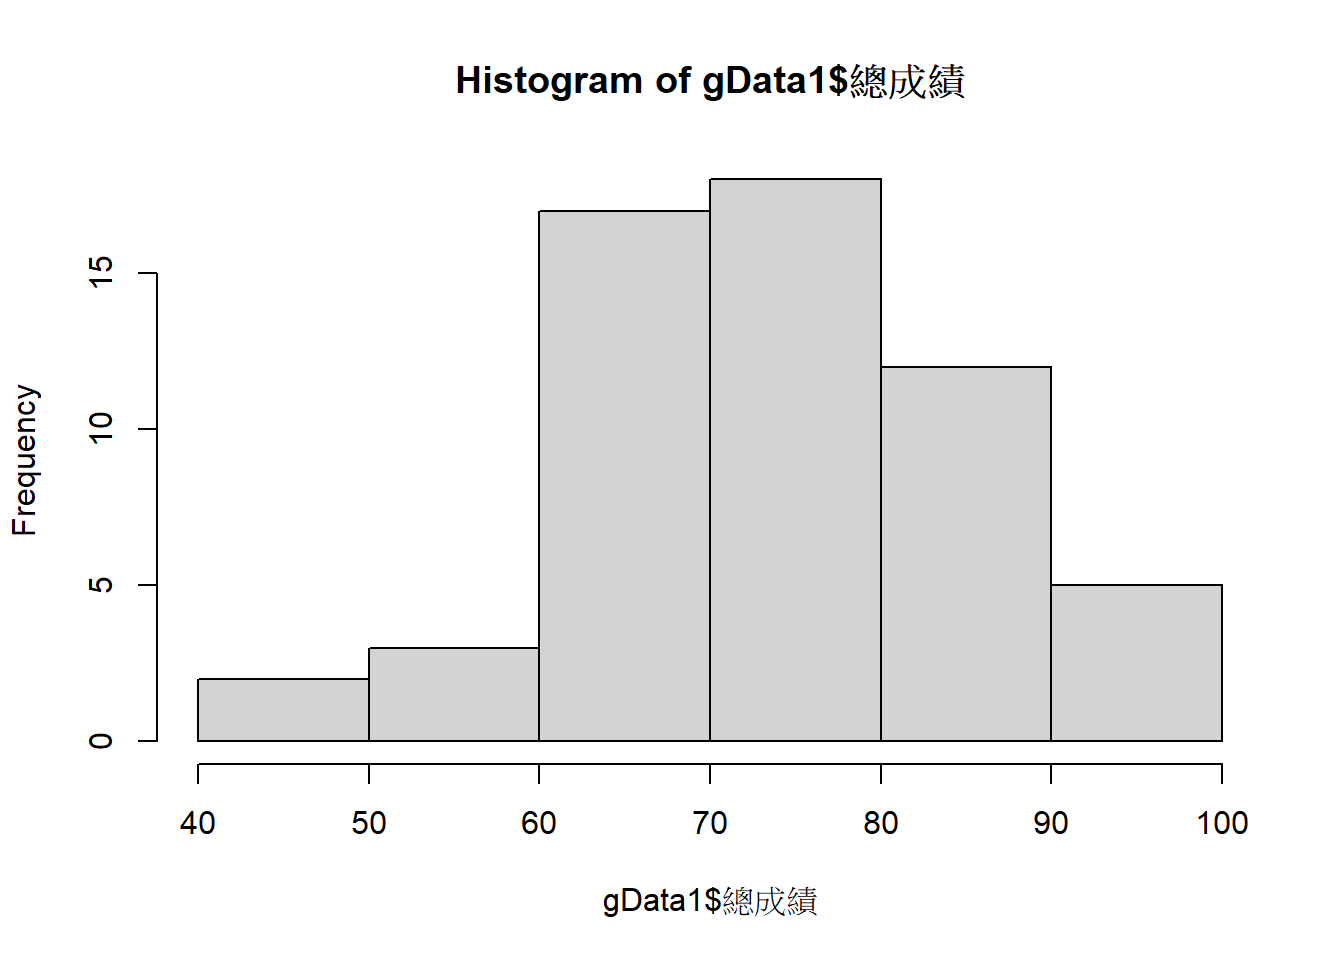
\includegraphics{quick-r-statistics_files/figure-latex/unnamed-chunk-39-1.pdf}

\hypertarget{ux7bb1ux578bux5716}{%
\subsection{箱型圖}\label{ux7bb1ux578bux5716}}

以boxplot()來繪製箱型圖。

\begin{Shaded}
\begin{Highlighting}[]
\FunctionTok{boxplot}\NormalTok{(gData1}\SpecialCharTok{$}\NormalTok{總成績, }\AttributeTok{ylab=}\StringTok{"分"}\NormalTok{)}
\end{Highlighting}
\end{Shaded}

\begin{verbatim}
## Warning in (function (main = NULL, sub = NULL, xlab = NULL, ylab = NULL, :
## conversion failure on '分' in 'mbcsToSbcs': dot substituted for <e5>
\end{verbatim}

\begin{verbatim}
## Warning in (function (main = NULL, sub = NULL, xlab = NULL, ylab = NULL, :
## conversion failure on '分' in 'mbcsToSbcs': dot substituted for <88>
\end{verbatim}

\begin{verbatim}
## Warning in (function (main = NULL, sub = NULL, xlab = NULL, ylab = NULL, :
## conversion failure on '分' in 'mbcsToSbcs': dot substituted for <86>
\end{verbatim}

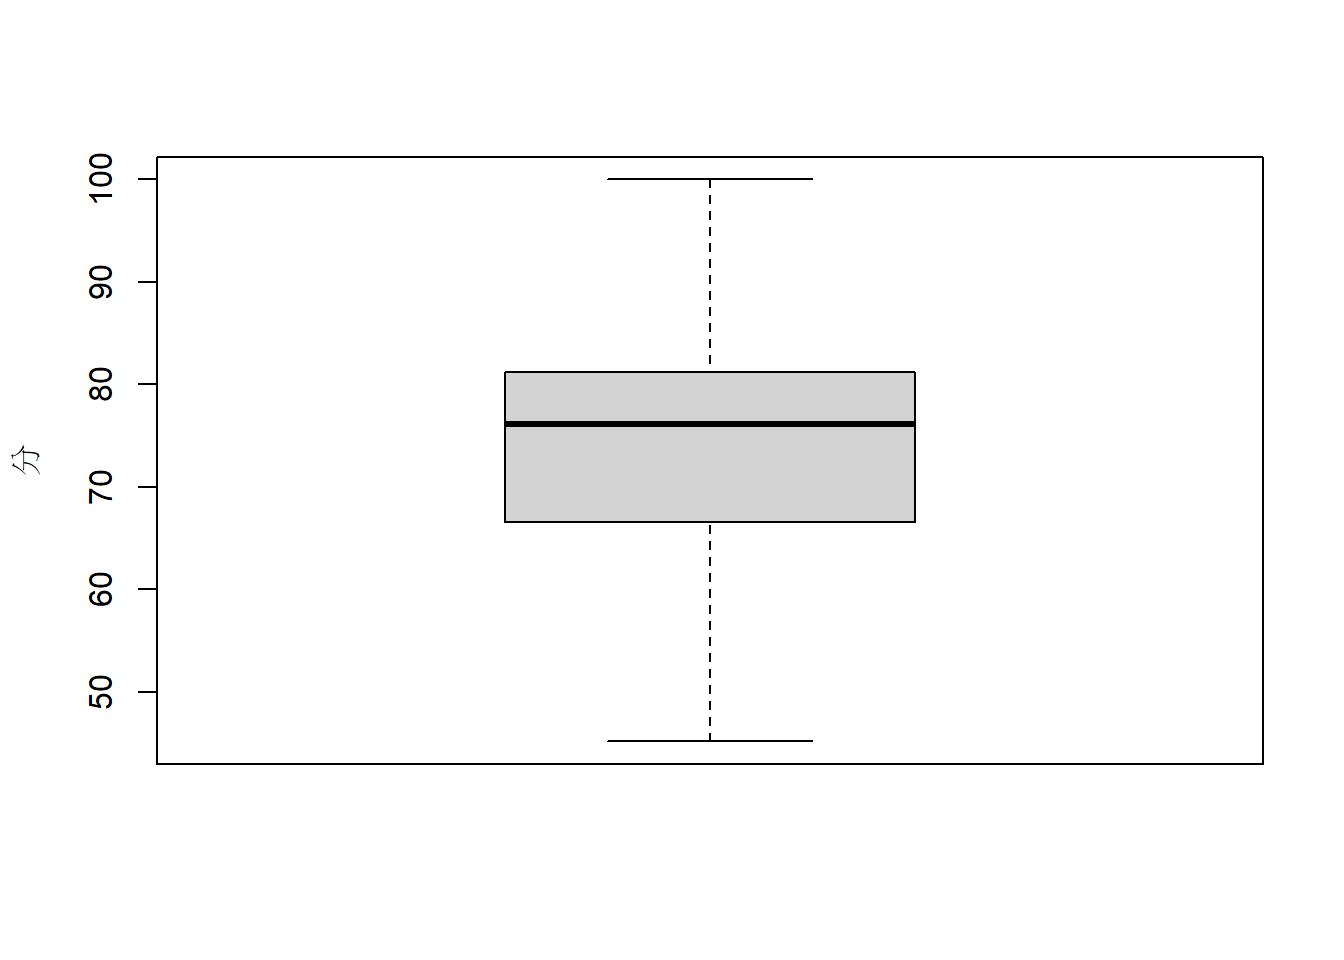
\includegraphics{quick-r-statistics_files/figure-latex/unnamed-chunk-40-1.pdf}

分組畫箱型圖。

\begin{Shaded}
\begin{Highlighting}[]
\FunctionTok{boxplot}\NormalTok{(gData1}\SpecialCharTok{$}\NormalTok{總成績}\SpecialCharTok{\textasciitilde{}}\NormalTok{gData1}\SpecialCharTok{$}\NormalTok{性別, }\AttributeTok{xlab=}\StringTok{"性別"}\NormalTok{, }\AttributeTok{ylab=}\StringTok{"分"}\NormalTok{)}
\end{Highlighting}
\end{Shaded}

\begin{verbatim}
## Warning in (function (main = NULL, sub = NULL, xlab = NULL, ylab = NULL, :
## conversion failure on '性別' in 'mbcsToSbcs': dot substituted for <e6>
\end{verbatim}

\begin{verbatim}
## Warning in (function (main = NULL, sub = NULL, xlab = NULL, ylab = NULL, :
## conversion failure on '性別' in 'mbcsToSbcs': dot substituted for <80>
\end{verbatim}

\begin{verbatim}
## Warning in (function (main = NULL, sub = NULL, xlab = NULL, ylab = NULL, :
## conversion failure on '性別' in 'mbcsToSbcs': dot substituted for <a7>
\end{verbatim}

\begin{verbatim}
## Warning in (function (main = NULL, sub = NULL, xlab = NULL, ylab = NULL, :
## conversion failure on '性別' in 'mbcsToSbcs': dot substituted for <e5>
\end{verbatim}

\begin{verbatim}
## Warning in (function (main = NULL, sub = NULL, xlab = NULL, ylab = NULL, :
## conversion failure on '性別' in 'mbcsToSbcs': dot substituted for <88>
\end{verbatim}

\begin{verbatim}
## Warning in (function (main = NULL, sub = NULL, xlab = NULL, ylab = NULL, :
## conversion failure on '性別' in 'mbcsToSbcs': dot substituted for <a5>
\end{verbatim}

\begin{verbatim}
## Warning in (function (main = NULL, sub = NULL, xlab = NULL, ylab = NULL, :
## conversion failure on '分' in 'mbcsToSbcs': dot substituted for <e5>
\end{verbatim}

\begin{verbatim}
## Warning in (function (main = NULL, sub = NULL, xlab = NULL, ylab = NULL, :
## conversion failure on '分' in 'mbcsToSbcs': dot substituted for <88>
\end{verbatim}

\begin{verbatim}
## Warning in (function (main = NULL, sub = NULL, xlab = NULL, ylab = NULL, :
## conversion failure on '分' in 'mbcsToSbcs': dot substituted for <86>
\end{verbatim}

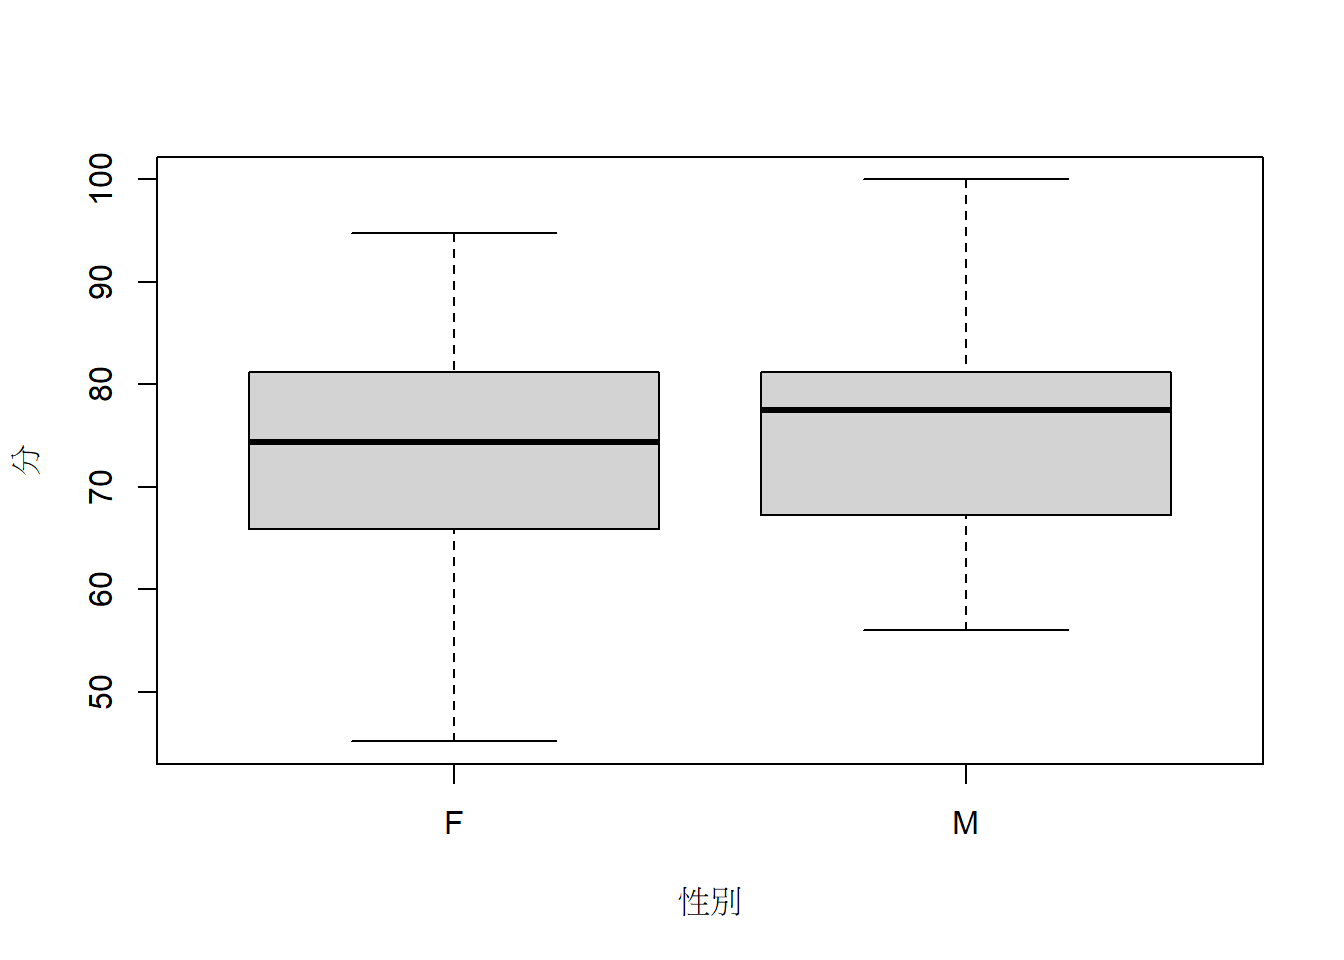
\includegraphics{quick-r-statistics_files/figure-latex/unnamed-chunk-41-1.pdf}

\hypertarget{ux6563ux4f48ux5716}{%
\subsection{散佈圖}\label{ux6563ux4f48ux5716}}

以plot()繪製兩變項或多個變項的散佈圖。

\begin{Shaded}
\begin{Highlighting}[]
\FunctionTok{plot}\NormalTok{(gData1}\SpecialCharTok{$}\NormalTok{出席, gData1}\SpecialCharTok{$}\NormalTok{總成績, }\AttributeTok{xlab=}\StringTok{"出席"}\NormalTok{, }\AttributeTok{ylab=}\StringTok{"總成績"}\NormalTok{)}
\end{Highlighting}
\end{Shaded}

\begin{verbatim}
## Warning in title(...): conversion failure on '出席' in 'mbcsToSbcs': dot
## substituted for <e5>
\end{verbatim}

\begin{verbatim}
## Warning in title(...): conversion failure on '出席' in 'mbcsToSbcs': dot
## substituted for <87>
\end{verbatim}

\begin{verbatim}
## Warning in title(...): conversion failure on '出席' in 'mbcsToSbcs': dot
## substituted for <ba>
\end{verbatim}

\begin{verbatim}
## Warning in title(...): conversion failure on '出席' in 'mbcsToSbcs': dot
## substituted for <e5>
\end{verbatim}

\begin{verbatim}
## Warning in title(...): conversion failure on '出席' in 'mbcsToSbcs': dot
## substituted for <b8>
\end{verbatim}

\begin{verbatim}
## Warning in title(...): conversion failure on '出席' in 'mbcsToSbcs': dot
## substituted for <ad>
\end{verbatim}

\begin{verbatim}
## Warning in title(...): conversion failure on '總成績' in 'mbcsToSbcs': dot
## substituted for <e7>
\end{verbatim}

\begin{verbatim}
## Warning in title(...): conversion failure on '總成績' in 'mbcsToSbcs': dot
## substituted for <b8>
\end{verbatim}

\begin{verbatim}
## Warning in title(...): conversion failure on '總成績' in 'mbcsToSbcs': dot
## substituted for <bd>
\end{verbatim}

\begin{verbatim}
## Warning in title(...): conversion failure on '總成績' in 'mbcsToSbcs': dot
## substituted for <e6>
\end{verbatim}

\begin{verbatim}
## Warning in title(...): conversion failure on '總成績' in 'mbcsToSbcs': dot
## substituted for <88>
\end{verbatim}

\begin{verbatim}
## Warning in title(...): conversion failure on '總成績' in 'mbcsToSbcs': dot
## substituted for <90>
\end{verbatim}

\begin{verbatim}
## Warning in title(...): conversion failure on '總成績' in 'mbcsToSbcs': dot
## substituted for <e7>
\end{verbatim}

\begin{verbatim}
## Warning in title(...): conversion failure on '總成績' in 'mbcsToSbcs': dot
## substituted for <b8>
\end{verbatim}

\begin{verbatim}
## Warning in title(...): conversion failure on '總成績' in 'mbcsToSbcs': dot
## substituted for <be>
\end{verbatim}

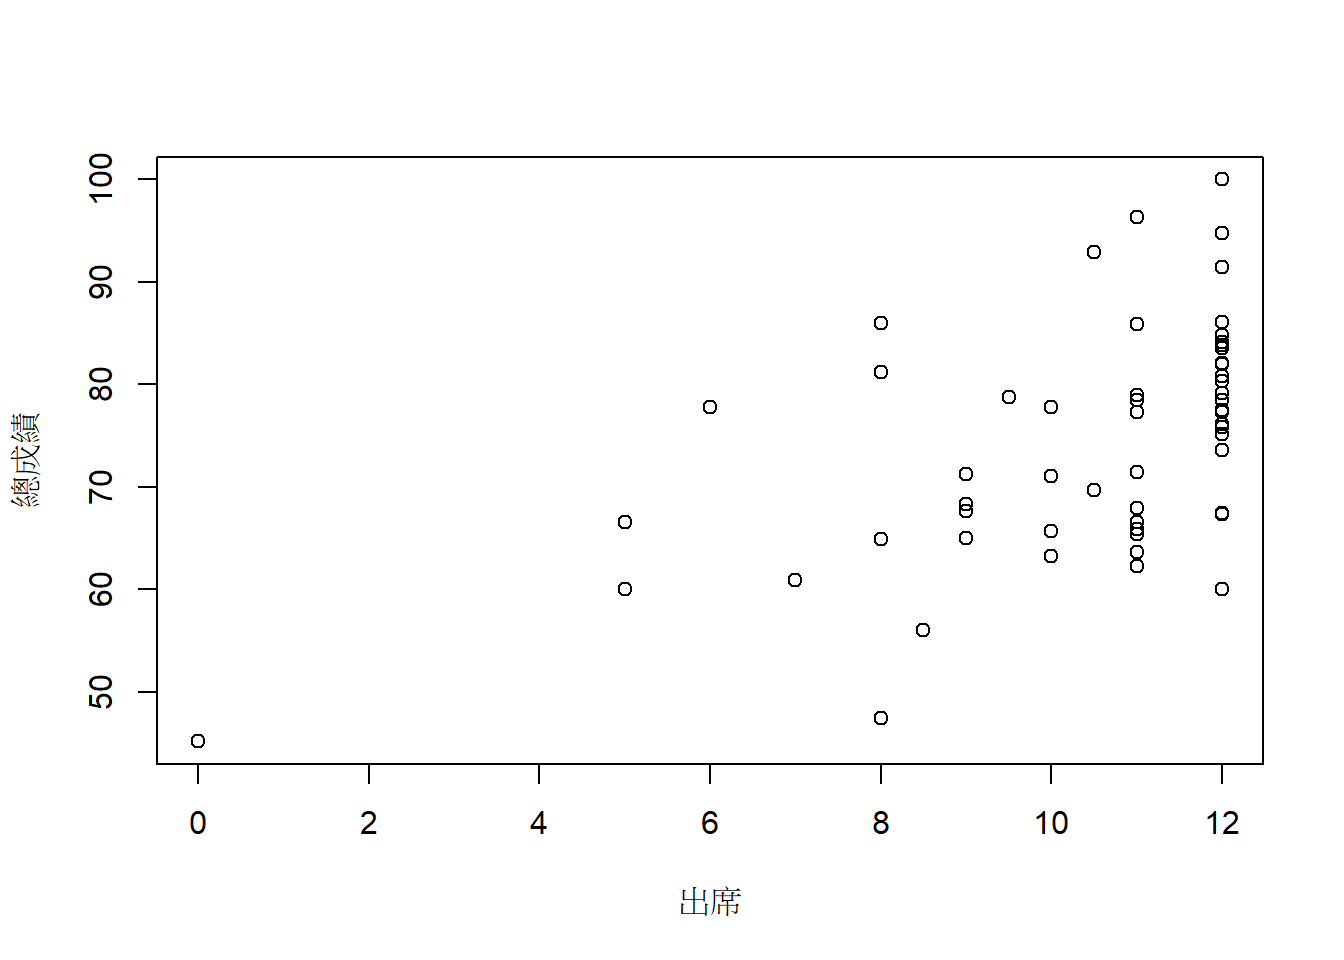
\includegraphics{quick-r-statistics_files/figure-latex/unnamed-chunk-42-1.pdf}

\begin{Shaded}
\begin{Highlighting}[]
\NormalTok{gData2 }\OtherTok{\textless{}{-}} \FunctionTok{subset}\NormalTok{(gData1, }\AttributeTok{select =} \FunctionTok{c}\NormalTok{(出席, 期中考, 期末考, 總成績))}
\FunctionTok{plot}\NormalTok{(gData2)}
\end{Highlighting}
\end{Shaded}

\begin{verbatim}
## Warning in strwidth(labels, "user"): conversion failure on '出席' in
## 'mbcsToSbcs': dot substituted for <e5>
\end{verbatim}

\begin{verbatim}
## Warning in strwidth(labels, "user"): conversion failure on '出席' in
## 'mbcsToSbcs': dot substituted for <87>
\end{verbatim}

\begin{verbatim}
## Warning in strwidth(labels, "user"): conversion failure on '出席' in
## 'mbcsToSbcs': dot substituted for <ba>
\end{verbatim}

\begin{verbatim}
## Warning in strwidth(labels, "user"): conversion failure on '出席' in
## 'mbcsToSbcs': dot substituted for <e5>
\end{verbatim}

\begin{verbatim}
## Warning in strwidth(labels, "user"): conversion failure on '出席' in
## 'mbcsToSbcs': dot substituted for <b8>
\end{verbatim}

\begin{verbatim}
## Warning in strwidth(labels, "user"): conversion failure on '出席' in
## 'mbcsToSbcs': dot substituted for <ad>
\end{verbatim}

\begin{verbatim}
## Warning in strwidth(labels, "user"): conversion failure on '期中考' in
## 'mbcsToSbcs': dot substituted for <e6>
\end{verbatim}

\begin{verbatim}
## Warning in strwidth(labels, "user"): conversion failure on '期中考' in
## 'mbcsToSbcs': dot substituted for <9c>
\end{verbatim}

\begin{verbatim}
## Warning in strwidth(labels, "user"): conversion failure on '期中考' in
## 'mbcsToSbcs': dot substituted for <9f>
\end{verbatim}

\begin{verbatim}
## Warning in strwidth(labels, "user"): conversion failure on '期中考' in
## 'mbcsToSbcs': dot substituted for <e4>
\end{verbatim}

\begin{verbatim}
## Warning in strwidth(labels, "user"): conversion failure on '期中考' in
## 'mbcsToSbcs': dot substituted for <b8>
\end{verbatim}

\begin{verbatim}
## Warning in strwidth(labels, "user"): conversion failure on '期中考' in
## 'mbcsToSbcs': dot substituted for <ad>
\end{verbatim}

\begin{verbatim}
## Warning in strwidth(labels, "user"): conversion failure on '期中考' in
## 'mbcsToSbcs': dot substituted for <e8>
\end{verbatim}

\begin{verbatim}
## Warning in strwidth(labels, "user"): conversion failure on '期中考' in
## 'mbcsToSbcs': dot substituted for <80>
\end{verbatim}

\begin{verbatim}
## Warning in strwidth(labels, "user"): conversion failure on '期中考' in
## 'mbcsToSbcs': dot substituted for <83>
\end{verbatim}

\begin{verbatim}
## Warning in strwidth(labels, "user"): conversion failure on '期末考' in
## 'mbcsToSbcs': dot substituted for <e6>
\end{verbatim}

\begin{verbatim}
## Warning in strwidth(labels, "user"): conversion failure on '期末考' in
## 'mbcsToSbcs': dot substituted for <9c>
\end{verbatim}

\begin{verbatim}
## Warning in strwidth(labels, "user"): conversion failure on '期末考' in
## 'mbcsToSbcs': dot substituted for <9f>
\end{verbatim}

\begin{verbatim}
## Warning in strwidth(labels, "user"): conversion failure on '期末考' in
## 'mbcsToSbcs': dot substituted for <e6>
\end{verbatim}

\begin{verbatim}
## Warning in strwidth(labels, "user"): conversion failure on '期末考' in
## 'mbcsToSbcs': dot substituted for <9c>
\end{verbatim}

\begin{verbatim}
## Warning in strwidth(labels, "user"): conversion failure on '期末考' in
## 'mbcsToSbcs': dot substituted for <ab>
\end{verbatim}

\begin{verbatim}
## Warning in strwidth(labels, "user"): conversion failure on '期末考' in
## 'mbcsToSbcs': dot substituted for <e8>
\end{verbatim}

\begin{verbatim}
## Warning in strwidth(labels, "user"): conversion failure on '期末考' in
## 'mbcsToSbcs': dot substituted for <80>
\end{verbatim}

\begin{verbatim}
## Warning in strwidth(labels, "user"): conversion failure on '期末考' in
## 'mbcsToSbcs': dot substituted for <83>
\end{verbatim}

\begin{verbatim}
## Warning in strwidth(labels, "user"): conversion failure on '總成績' in
## 'mbcsToSbcs': dot substituted for <e7>
\end{verbatim}

\begin{verbatim}
## Warning in strwidth(labels, "user"): conversion failure on '總成績' in
## 'mbcsToSbcs': dot substituted for <b8>
\end{verbatim}

\begin{verbatim}
## Warning in strwidth(labels, "user"): conversion failure on '總成績' in
## 'mbcsToSbcs': dot substituted for <bd>
\end{verbatim}

\begin{verbatim}
## Warning in strwidth(labels, "user"): conversion failure on '總成績' in
## 'mbcsToSbcs': dot substituted for <e6>
\end{verbatim}

\begin{verbatim}
## Warning in strwidth(labels, "user"): conversion failure on '總成績' in
## 'mbcsToSbcs': dot substituted for <88>
\end{verbatim}

\begin{verbatim}
## Warning in strwidth(labels, "user"): conversion failure on '總成績' in
## 'mbcsToSbcs': dot substituted for <90>
\end{verbatim}

\begin{verbatim}
## Warning in strwidth(labels, "user"): conversion failure on '總成績' in
## 'mbcsToSbcs': dot substituted for <e7>
\end{verbatim}

\begin{verbatim}
## Warning in strwidth(labels, "user"): conversion failure on '總成績' in
## 'mbcsToSbcs': dot substituted for <b8>
\end{verbatim}

\begin{verbatim}
## Warning in strwidth(labels, "user"): conversion failure on '總成績' in
## 'mbcsToSbcs': dot substituted for <be>
\end{verbatim}

\begin{verbatim}
## Warning in text.default(x, y, txt, cex = cex, font = font): conversion failure
## on '出席' in 'mbcsToSbcs': dot substituted for <e5>
\end{verbatim}

\begin{verbatim}
## Warning in text.default(x, y, txt, cex = cex, font = font): conversion failure
## on '出席' in 'mbcsToSbcs': dot substituted for <87>
\end{verbatim}

\begin{verbatim}
## Warning in text.default(x, y, txt, cex = cex, font = font): conversion failure
## on '出席' in 'mbcsToSbcs': dot substituted for <ba>
\end{verbatim}

\begin{verbatim}
## Warning in text.default(x, y, txt, cex = cex, font = font): conversion failure
## on '出席' in 'mbcsToSbcs': dot substituted for <e5>
\end{verbatim}

\begin{verbatim}
## Warning in text.default(x, y, txt, cex = cex, font = font): conversion failure
## on '出席' in 'mbcsToSbcs': dot substituted for <b8>
\end{verbatim}

\begin{verbatim}
## Warning in text.default(x, y, txt, cex = cex, font = font): conversion failure
## on '出席' in 'mbcsToSbcs': dot substituted for <ad>
\end{verbatim}

\begin{verbatim}
## Warning in text.default(x, y, txt, cex = cex, font = font): font metrics unknown
## for Unicode character U+51fa
\end{verbatim}

\begin{verbatim}
## Warning in text.default(x, y, txt, cex = cex, font = font): font metrics unknown
## for Unicode character U+5e2d
\end{verbatim}

\begin{verbatim}
## Warning in text.default(x, y, txt, cex = cex, font = font): conversion failure
## on '期中考' in 'mbcsToSbcs': dot substituted for <e6>
\end{verbatim}

\begin{verbatim}
## Warning in text.default(x, y, txt, cex = cex, font = font): conversion failure
## on '期中考' in 'mbcsToSbcs': dot substituted for <9c>
\end{verbatim}

\begin{verbatim}
## Warning in text.default(x, y, txt, cex = cex, font = font): conversion failure
## on '期中考' in 'mbcsToSbcs': dot substituted for <9f>
\end{verbatim}

\begin{verbatim}
## Warning in text.default(x, y, txt, cex = cex, font = font): conversion failure
## on '期中考' in 'mbcsToSbcs': dot substituted for <e4>
\end{verbatim}

\begin{verbatim}
## Warning in text.default(x, y, txt, cex = cex, font = font): conversion failure
## on '期中考' in 'mbcsToSbcs': dot substituted for <b8>
\end{verbatim}

\begin{verbatim}
## Warning in text.default(x, y, txt, cex = cex, font = font): conversion failure
## on '期中考' in 'mbcsToSbcs': dot substituted for <ad>
\end{verbatim}

\begin{verbatim}
## Warning in text.default(x, y, txt, cex = cex, font = font): conversion failure
## on '期中考' in 'mbcsToSbcs': dot substituted for <e8>
\end{verbatim}

\begin{verbatim}
## Warning in text.default(x, y, txt, cex = cex, font = font): conversion failure
## on '期中考' in 'mbcsToSbcs': dot substituted for <80>
\end{verbatim}

\begin{verbatim}
## Warning in text.default(x, y, txt, cex = cex, font = font): conversion failure
## on '期中考' in 'mbcsToSbcs': dot substituted for <83>
\end{verbatim}

\begin{verbatim}
## Warning in text.default(x, y, txt, cex = cex, font = font): font metrics unknown
## for Unicode character U+671f
\end{verbatim}

\begin{verbatim}
## Warning in text.default(x, y, txt, cex = cex, font = font): font metrics unknown
## for Unicode character U+4e2d
\end{verbatim}

\begin{verbatim}
## Warning in text.default(x, y, txt, cex = cex, font = font): font metrics unknown
## for Unicode character U+8003
\end{verbatim}

\begin{verbatim}
## Warning in text.default(x, y, txt, cex = cex, font = font): conversion failure
## on '期末考' in 'mbcsToSbcs': dot substituted for <e6>
\end{verbatim}

\begin{verbatim}
## Warning in text.default(x, y, txt, cex = cex, font = font): conversion failure
## on '期末考' in 'mbcsToSbcs': dot substituted for <9c>
\end{verbatim}

\begin{verbatim}
## Warning in text.default(x, y, txt, cex = cex, font = font): conversion failure
## on '期末考' in 'mbcsToSbcs': dot substituted for <9f>
\end{verbatim}

\begin{verbatim}
## Warning in text.default(x, y, txt, cex = cex, font = font): conversion failure
## on '期末考' in 'mbcsToSbcs': dot substituted for <e6>
\end{verbatim}

\begin{verbatim}
## Warning in text.default(x, y, txt, cex = cex, font = font): conversion failure
## on '期末考' in 'mbcsToSbcs': dot substituted for <9c>
\end{verbatim}

\begin{verbatim}
## Warning in text.default(x, y, txt, cex = cex, font = font): conversion failure
## on '期末考' in 'mbcsToSbcs': dot substituted for <ab>
\end{verbatim}

\begin{verbatim}
## Warning in text.default(x, y, txt, cex = cex, font = font): conversion failure
## on '期末考' in 'mbcsToSbcs': dot substituted for <e8>
\end{verbatim}

\begin{verbatim}
## Warning in text.default(x, y, txt, cex = cex, font = font): conversion failure
## on '期末考' in 'mbcsToSbcs': dot substituted for <80>
\end{verbatim}

\begin{verbatim}
## Warning in text.default(x, y, txt, cex = cex, font = font): conversion failure
## on '期末考' in 'mbcsToSbcs': dot substituted for <83>
\end{verbatim}

\begin{verbatim}
## Warning in text.default(x, y, txt, cex = cex, font = font): font metrics unknown
## for Unicode character U+671f
\end{verbatim}

\begin{verbatim}
## Warning in text.default(x, y, txt, cex = cex, font = font): font metrics unknown
## for Unicode character U+672b
\end{verbatim}

\begin{verbatim}
## Warning in text.default(x, y, txt, cex = cex, font = font): font metrics unknown
## for Unicode character U+8003
\end{verbatim}

\begin{verbatim}
## Warning in text.default(x, y, txt, cex = cex, font = font): conversion failure
## on '總成績' in 'mbcsToSbcs': dot substituted for <e7>
\end{verbatim}

\begin{verbatim}
## Warning in text.default(x, y, txt, cex = cex, font = font): conversion failure
## on '總成績' in 'mbcsToSbcs': dot substituted for <b8>
\end{verbatim}

\begin{verbatim}
## Warning in text.default(x, y, txt, cex = cex, font = font): conversion failure
## on '總成績' in 'mbcsToSbcs': dot substituted for <bd>
\end{verbatim}

\begin{verbatim}
## Warning in text.default(x, y, txt, cex = cex, font = font): conversion failure
## on '總成績' in 'mbcsToSbcs': dot substituted for <e6>
\end{verbatim}

\begin{verbatim}
## Warning in text.default(x, y, txt, cex = cex, font = font): conversion failure
## on '總成績' in 'mbcsToSbcs': dot substituted for <88>
\end{verbatim}

\begin{verbatim}
## Warning in text.default(x, y, txt, cex = cex, font = font): conversion failure
## on '總成績' in 'mbcsToSbcs': dot substituted for <90>
\end{verbatim}

\begin{verbatim}
## Warning in text.default(x, y, txt, cex = cex, font = font): conversion failure
## on '總成績' in 'mbcsToSbcs': dot substituted for <e7>
\end{verbatim}

\begin{verbatim}
## Warning in text.default(x, y, txt, cex = cex, font = font): conversion failure
## on '總成績' in 'mbcsToSbcs': dot substituted for <b8>
\end{verbatim}

\begin{verbatim}
## Warning in text.default(x, y, txt, cex = cex, font = font): conversion failure
## on '總成績' in 'mbcsToSbcs': dot substituted for <be>
\end{verbatim}

\begin{verbatim}
## Warning in text.default(x, y, txt, cex = cex, font = font): font metrics unknown
## for Unicode character U+7e3d
\end{verbatim}

\begin{verbatim}
## Warning in text.default(x, y, txt, cex = cex, font = font): font metrics unknown
## for Unicode character U+6210
\end{verbatim}

\begin{verbatim}
## Warning in text.default(x, y, txt, cex = cex, font = font): font metrics unknown
## for Unicode character U+7e3e
\end{verbatim}

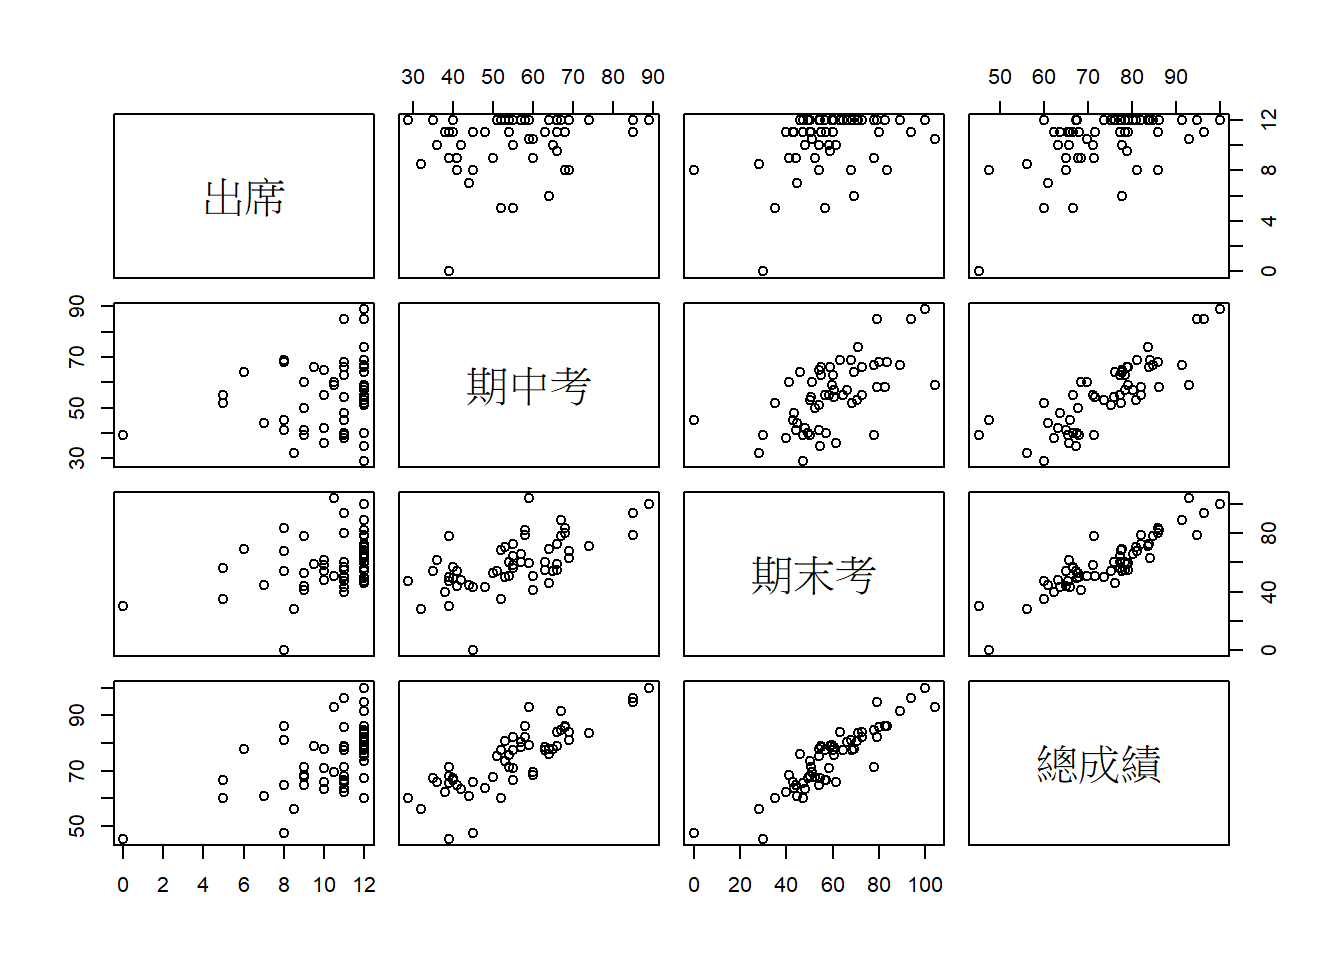
\includegraphics{quick-r-statistics_files/figure-latex/unnamed-chunk-43-1.pdf}

\hypertarget{ux8a08ux7b97ux76f8ux95dcux8207ux7e6aux5716}{%
\subsection{計算相關與繪圖}\label{ux8a08ux7b97ux76f8ux95dcux8207ux7e6aux5716}}

\hypertarget{ux8a08ux7b97ux76f8ux95dc}{%
\subsubsection{計算相關}\label{ux8a08ux7b97ux76f8ux95dc}}

以cor()計算兩變項的相關,或以cor.test()得到相關和檢定值。

\begin{Shaded}
\begin{Highlighting}[]
\FunctionTok{cor}\NormalTok{(gData1}\SpecialCharTok{$}\NormalTok{出席, gData1}\SpecialCharTok{$}\NormalTok{總成績)}
\end{Highlighting}
\end{Shaded}

\begin{verbatim}
## [1] 0.5360227
\end{verbatim}

\begin{Shaded}
\begin{Highlighting}[]
\FunctionTok{cor.test}\NormalTok{(gData1}\SpecialCharTok{$}\NormalTok{出席, gData1}\SpecialCharTok{$}\NormalTok{總成績)}
\end{Highlighting}
\end{Shaded}

\begin{verbatim}
## 
##  Pearson's product-moment correlation
## 
## data:  gData1$出席 and gData1$總成績
## t = 4.7089, df = 55, p-value = 1.73e-05
## alternative hypothesis: true correlation is not equal to 0
## 95 percent confidence interval:
##  0.3201738 0.6989657
## sample estimates:
##       cor 
## 0.5360227
\end{verbatim}

cor()可計算多個變項的相關,若要得到檢定結果,可用Hmisc()的rcorr()函數。

\begin{Shaded}
\begin{Highlighting}[]
\FunctionTok{cor}\NormalTok{(gData2)}
\end{Highlighting}
\end{Shaded}

\begin{verbatim}
##             出席    期中考    期末考    總成績
## 出席   1.0000000 0.2220785 0.3760520 0.5360227
## 期中考 0.2220785 1.0000000 0.6211838 0.8319727
## 期末考 0.3760520 0.6211838 1.0000000 0.8983073
## 總成績 0.5360227 0.8319727 0.8983073 1.0000000
\end{verbatim}

\begin{Shaded}
\begin{Highlighting}[]
\FunctionTok{library}\NormalTok{(Hmisc)}
\FunctionTok{rcorr}\NormalTok{(}\FunctionTok{data.matrix}\NormalTok{(gData2))}
\end{Highlighting}
\end{Shaded}

\begin{verbatim}
##        出席 期中考 期末考 總成績
## 出席   1.00   0.22   0.38   0.54
## 期中考 0.22   1.00   0.62   0.83
## 期末考 0.38   0.62   1.00   0.90
## 總成績 0.54   0.83   0.90   1.00
## 
## n= 57 
## 
## 
## P
##        出席   期中考 期末考 總成績
## 出席          0.0969 0.0039 0.0000
## 期中考 0.0969        0.0000 0.0000
## 期末考 0.0039 0.0000        0.0000
## 總成績 0.0000 0.0000 0.0000
\end{verbatim}

\hypertarget{ux591aux500bux8b8aux9805ux7684ux76f8ux95dcux77e9ux9663ux5716}{%
\subsubsection{多個變項的相關矩陣圖}\label{ux591aux500bux8b8aux9805ux7684ux76f8ux95dcux77e9ux9663ux5716}}

若要將多個變項的相關視覺化,可使用corrplot套件的corrplot()函數。

\begin{Shaded}
\begin{Highlighting}[]
\FunctionTok{library}\NormalTok{(corrplot)}
\FunctionTok{corrplot}\NormalTok{(}\FunctionTok{cor}\NormalTok{(gData2), }\AttributeTok{method=}\StringTok{\textquotesingle{}number\textquotesingle{}}\NormalTok{,}\AttributeTok{type =} \StringTok{"upper"}\NormalTok{)}
\end{Highlighting}
\end{Shaded}

\begin{verbatim}
## Warning in strwidth(newrownames, cex = tl.cex): conversion failure on '出席' in
## 'mbcsToSbcs': dot substituted for <e5>
\end{verbatim}

\begin{verbatim}
## Warning in strwidth(newrownames, cex = tl.cex): conversion failure on '出席' in
## 'mbcsToSbcs': dot substituted for <87>
\end{verbatim}

\begin{verbatim}
## Warning in strwidth(newrownames, cex = tl.cex): conversion failure on '出席' in
## 'mbcsToSbcs': dot substituted for <ba>
\end{verbatim}

\begin{verbatim}
## Warning in strwidth(newrownames, cex = tl.cex): conversion failure on '出席' in
## 'mbcsToSbcs': dot substituted for <e5>
\end{verbatim}

\begin{verbatim}
## Warning in strwidth(newrownames, cex = tl.cex): conversion failure on '出席' in
## 'mbcsToSbcs': dot substituted for <b8>
\end{verbatim}

\begin{verbatim}
## Warning in strwidth(newrownames, cex = tl.cex): conversion failure on '出席' in
## 'mbcsToSbcs': dot substituted for <ad>
\end{verbatim}

\begin{verbatim}
## Warning in strwidth(newrownames, cex = tl.cex): conversion failure on '期中考'
## in 'mbcsToSbcs': dot substituted for <e6>
\end{verbatim}

\begin{verbatim}
## Warning in strwidth(newrownames, cex = tl.cex): conversion failure on '期中考'
## in 'mbcsToSbcs': dot substituted for <9c>
\end{verbatim}

\begin{verbatim}
## Warning in strwidth(newrownames, cex = tl.cex): conversion failure on '期中考'
## in 'mbcsToSbcs': dot substituted for <9f>
\end{verbatim}

\begin{verbatim}
## Warning in strwidth(newrownames, cex = tl.cex): conversion failure on '期中考'
## in 'mbcsToSbcs': dot substituted for <e4>
\end{verbatim}

\begin{verbatim}
## Warning in strwidth(newrownames, cex = tl.cex): conversion failure on '期中考'
## in 'mbcsToSbcs': dot substituted for <b8>
\end{verbatim}

\begin{verbatim}
## Warning in strwidth(newrownames, cex = tl.cex): conversion failure on '期中考'
## in 'mbcsToSbcs': dot substituted for <ad>
\end{verbatim}

\begin{verbatim}
## Warning in strwidth(newrownames, cex = tl.cex): conversion failure on '期中考'
## in 'mbcsToSbcs': dot substituted for <e8>
\end{verbatim}

\begin{verbatim}
## Warning in strwidth(newrownames, cex = tl.cex): conversion failure on '期中考'
## in 'mbcsToSbcs': dot substituted for <80>
\end{verbatim}

\begin{verbatim}
## Warning in strwidth(newrownames, cex = tl.cex): conversion failure on '期中考'
## in 'mbcsToSbcs': dot substituted for <83>
\end{verbatim}

\begin{verbatim}
## Warning in strwidth(newrownames, cex = tl.cex): conversion failure on '期末考'
## in 'mbcsToSbcs': dot substituted for <e6>
\end{verbatim}

\begin{verbatim}
## Warning in strwidth(newrownames, cex = tl.cex): conversion failure on '期末考'
## in 'mbcsToSbcs': dot substituted for <9c>
\end{verbatim}

\begin{verbatim}
## Warning in strwidth(newrownames, cex = tl.cex): conversion failure on '期末考'
## in 'mbcsToSbcs': dot substituted for <9f>
\end{verbatim}

\begin{verbatim}
## Warning in strwidth(newrownames, cex = tl.cex): conversion failure on '期末考'
## in 'mbcsToSbcs': dot substituted for <e6>
\end{verbatim}

\begin{verbatim}
## Warning in strwidth(newrownames, cex = tl.cex): conversion failure on '期末考'
## in 'mbcsToSbcs': dot substituted for <9c>
\end{verbatim}

\begin{verbatim}
## Warning in strwidth(newrownames, cex = tl.cex): conversion failure on '期末考'
## in 'mbcsToSbcs': dot substituted for <ab>
\end{verbatim}

\begin{verbatim}
## Warning in strwidth(newrownames, cex = tl.cex): conversion failure on '期末考'
## in 'mbcsToSbcs': dot substituted for <e8>
\end{verbatim}

\begin{verbatim}
## Warning in strwidth(newrownames, cex = tl.cex): conversion failure on '期末考'
## in 'mbcsToSbcs': dot substituted for <80>
\end{verbatim}

\begin{verbatim}
## Warning in strwidth(newrownames, cex = tl.cex): conversion failure on '期末考'
## in 'mbcsToSbcs': dot substituted for <83>
\end{verbatim}

\begin{verbatim}
## Warning in strwidth(newrownames, cex = tl.cex): conversion failure on '總成績'
## in 'mbcsToSbcs': dot substituted for <e7>
\end{verbatim}

\begin{verbatim}
## Warning in strwidth(newrownames, cex = tl.cex): conversion failure on '總成績'
## in 'mbcsToSbcs': dot substituted for <b8>
\end{verbatim}

\begin{verbatim}
## Warning in strwidth(newrownames, cex = tl.cex): conversion failure on '總成績'
## in 'mbcsToSbcs': dot substituted for <bd>
\end{verbatim}

\begin{verbatim}
## Warning in strwidth(newrownames, cex = tl.cex): conversion failure on '總成績'
## in 'mbcsToSbcs': dot substituted for <e6>
\end{verbatim}

\begin{verbatim}
## Warning in strwidth(newrownames, cex = tl.cex): conversion failure on '總成績'
## in 'mbcsToSbcs': dot substituted for <88>
\end{verbatim}

\begin{verbatim}
## Warning in strwidth(newrownames, cex = tl.cex): conversion failure on '總成績'
## in 'mbcsToSbcs': dot substituted for <90>
\end{verbatim}

\begin{verbatim}
## Warning in strwidth(newrownames, cex = tl.cex): conversion failure on '總成績'
## in 'mbcsToSbcs': dot substituted for <e7>
\end{verbatim}

\begin{verbatim}
## Warning in strwidth(newrownames, cex = tl.cex): conversion failure on '總成績'
## in 'mbcsToSbcs': dot substituted for <b8>
\end{verbatim}

\begin{verbatim}
## Warning in strwidth(newrownames, cex = tl.cex): conversion failure on '總成績'
## in 'mbcsToSbcs': dot substituted for <be>
\end{verbatim}

\begin{verbatim}
## Warning in strwidth(newcolnames, cex = tl.cex): conversion failure on '出席' in
## 'mbcsToSbcs': dot substituted for <e5>
\end{verbatim}

\begin{verbatim}
## Warning in strwidth(newcolnames, cex = tl.cex): conversion failure on '出席' in
## 'mbcsToSbcs': dot substituted for <87>
\end{verbatim}

\begin{verbatim}
## Warning in strwidth(newcolnames, cex = tl.cex): conversion failure on '出席' in
## 'mbcsToSbcs': dot substituted for <ba>
\end{verbatim}

\begin{verbatim}
## Warning in strwidth(newcolnames, cex = tl.cex): conversion failure on '出席' in
## 'mbcsToSbcs': dot substituted for <e5>
\end{verbatim}

\begin{verbatim}
## Warning in strwidth(newcolnames, cex = tl.cex): conversion failure on '出席' in
## 'mbcsToSbcs': dot substituted for <b8>
\end{verbatim}

\begin{verbatim}
## Warning in strwidth(newcolnames, cex = tl.cex): conversion failure on '出席' in
## 'mbcsToSbcs': dot substituted for <ad>
\end{verbatim}

\begin{verbatim}
## Warning in strwidth(newcolnames, cex = tl.cex): conversion failure on '期中考'
## in 'mbcsToSbcs': dot substituted for <e6>
\end{verbatim}

\begin{verbatim}
## Warning in strwidth(newcolnames, cex = tl.cex): conversion failure on '期中考'
## in 'mbcsToSbcs': dot substituted for <9c>
\end{verbatim}

\begin{verbatim}
## Warning in strwidth(newcolnames, cex = tl.cex): conversion failure on '期中考'
## in 'mbcsToSbcs': dot substituted for <9f>
\end{verbatim}

\begin{verbatim}
## Warning in strwidth(newcolnames, cex = tl.cex): conversion failure on '期中考'
## in 'mbcsToSbcs': dot substituted for <e4>
\end{verbatim}

\begin{verbatim}
## Warning in strwidth(newcolnames, cex = tl.cex): conversion failure on '期中考'
## in 'mbcsToSbcs': dot substituted for <b8>
\end{verbatim}

\begin{verbatim}
## Warning in strwidth(newcolnames, cex = tl.cex): conversion failure on '期中考'
## in 'mbcsToSbcs': dot substituted for <ad>
\end{verbatim}

\begin{verbatim}
## Warning in strwidth(newcolnames, cex = tl.cex): conversion failure on '期中考'
## in 'mbcsToSbcs': dot substituted for <e8>
\end{verbatim}

\begin{verbatim}
## Warning in strwidth(newcolnames, cex = tl.cex): conversion failure on '期中考'
## in 'mbcsToSbcs': dot substituted for <80>
\end{verbatim}

\begin{verbatim}
## Warning in strwidth(newcolnames, cex = tl.cex): conversion failure on '期中考'
## in 'mbcsToSbcs': dot substituted for <83>
\end{verbatim}

\begin{verbatim}
## Warning in strwidth(newcolnames, cex = tl.cex): conversion failure on '期末考'
## in 'mbcsToSbcs': dot substituted for <e6>
\end{verbatim}

\begin{verbatim}
## Warning in strwidth(newcolnames, cex = tl.cex): conversion failure on '期末考'
## in 'mbcsToSbcs': dot substituted for <9c>
\end{verbatim}

\begin{verbatim}
## Warning in strwidth(newcolnames, cex = tl.cex): conversion failure on '期末考'
## in 'mbcsToSbcs': dot substituted for <9f>
\end{verbatim}

\begin{verbatim}
## Warning in strwidth(newcolnames, cex = tl.cex): conversion failure on '期末考'
## in 'mbcsToSbcs': dot substituted for <e6>
\end{verbatim}

\begin{verbatim}
## Warning in strwidth(newcolnames, cex = tl.cex): conversion failure on '期末考'
## in 'mbcsToSbcs': dot substituted for <9c>
\end{verbatim}

\begin{verbatim}
## Warning in strwidth(newcolnames, cex = tl.cex): conversion failure on '期末考'
## in 'mbcsToSbcs': dot substituted for <ab>
\end{verbatim}

\begin{verbatim}
## Warning in strwidth(newcolnames, cex = tl.cex): conversion failure on '期末考'
## in 'mbcsToSbcs': dot substituted for <e8>
\end{verbatim}

\begin{verbatim}
## Warning in strwidth(newcolnames, cex = tl.cex): conversion failure on '期末考'
## in 'mbcsToSbcs': dot substituted for <80>
\end{verbatim}

\begin{verbatim}
## Warning in strwidth(newcolnames, cex = tl.cex): conversion failure on '期末考'
## in 'mbcsToSbcs': dot substituted for <83>
\end{verbatim}

\begin{verbatim}
## Warning in strwidth(newcolnames, cex = tl.cex): conversion failure on '總成績'
## in 'mbcsToSbcs': dot substituted for <e7>
\end{verbatim}

\begin{verbatim}
## Warning in strwidth(newcolnames, cex = tl.cex): conversion failure on '總成績'
## in 'mbcsToSbcs': dot substituted for <b8>
\end{verbatim}

\begin{verbatim}
## Warning in strwidth(newcolnames, cex = tl.cex): conversion failure on '總成績'
## in 'mbcsToSbcs': dot substituted for <bd>
\end{verbatim}

\begin{verbatim}
## Warning in strwidth(newcolnames, cex = tl.cex): conversion failure on '總成績'
## in 'mbcsToSbcs': dot substituted for <e6>
\end{verbatim}

\begin{verbatim}
## Warning in strwidth(newcolnames, cex = tl.cex): conversion failure on '總成績'
## in 'mbcsToSbcs': dot substituted for <88>
\end{verbatim}

\begin{verbatim}
## Warning in strwidth(newcolnames, cex = tl.cex): conversion failure on '總成績'
## in 'mbcsToSbcs': dot substituted for <90>
\end{verbatim}

\begin{verbatim}
## Warning in strwidth(newcolnames, cex = tl.cex): conversion failure on '總成績'
## in 'mbcsToSbcs': dot substituted for <e7>
\end{verbatim}

\begin{verbatim}
## Warning in strwidth(newcolnames, cex = tl.cex): conversion failure on '總成績'
## in 'mbcsToSbcs': dot substituted for <b8>
\end{verbatim}

\begin{verbatim}
## Warning in strwidth(newcolnames, cex = tl.cex): conversion failure on '總成績'
## in 'mbcsToSbcs': dot substituted for <be>
\end{verbatim}

\begin{verbatim}
## Warning in strwidth(newrownames, cex = tl.cex): conversion failure on '出席' in
## 'mbcsToSbcs': dot substituted for <e5>
\end{verbatim}

\begin{verbatim}
## Warning in strwidth(newrownames, cex = tl.cex): conversion failure on '出席' in
## 'mbcsToSbcs': dot substituted for <87>
\end{verbatim}

\begin{verbatim}
## Warning in strwidth(newrownames, cex = tl.cex): conversion failure on '出席' in
## 'mbcsToSbcs': dot substituted for <ba>
\end{verbatim}

\begin{verbatim}
## Warning in strwidth(newrownames, cex = tl.cex): conversion failure on '出席' in
## 'mbcsToSbcs': dot substituted for <e5>
\end{verbatim}

\begin{verbatim}
## Warning in strwidth(newrownames, cex = tl.cex): conversion failure on '出席' in
## 'mbcsToSbcs': dot substituted for <b8>
\end{verbatim}

\begin{verbatim}
## Warning in strwidth(newrownames, cex = tl.cex): conversion failure on '出席' in
## 'mbcsToSbcs': dot substituted for <ad>
\end{verbatim}

\begin{verbatim}
## Warning in strwidth(newrownames, cex = tl.cex): conversion failure on '期中考'
## in 'mbcsToSbcs': dot substituted for <e6>
\end{verbatim}

\begin{verbatim}
## Warning in strwidth(newrownames, cex = tl.cex): conversion failure on '期中考'
## in 'mbcsToSbcs': dot substituted for <9c>
\end{verbatim}

\begin{verbatim}
## Warning in strwidth(newrownames, cex = tl.cex): conversion failure on '期中考'
## in 'mbcsToSbcs': dot substituted for <9f>
\end{verbatim}

\begin{verbatim}
## Warning in strwidth(newrownames, cex = tl.cex): conversion failure on '期中考'
## in 'mbcsToSbcs': dot substituted for <e4>
\end{verbatim}

\begin{verbatim}
## Warning in strwidth(newrownames, cex = tl.cex): conversion failure on '期中考'
## in 'mbcsToSbcs': dot substituted for <b8>
\end{verbatim}

\begin{verbatim}
## Warning in strwidth(newrownames, cex = tl.cex): conversion failure on '期中考'
## in 'mbcsToSbcs': dot substituted for <ad>
\end{verbatim}

\begin{verbatim}
## Warning in strwidth(newrownames, cex = tl.cex): conversion failure on '期中考'
## in 'mbcsToSbcs': dot substituted for <e8>
\end{verbatim}

\begin{verbatim}
## Warning in strwidth(newrownames, cex = tl.cex): conversion failure on '期中考'
## in 'mbcsToSbcs': dot substituted for <80>
\end{verbatim}

\begin{verbatim}
## Warning in strwidth(newrownames, cex = tl.cex): conversion failure on '期中考'
## in 'mbcsToSbcs': dot substituted for <83>
\end{verbatim}

\begin{verbatim}
## Warning in strwidth(newrownames, cex = tl.cex): conversion failure on '期末考'
## in 'mbcsToSbcs': dot substituted for <e6>
\end{verbatim}

\begin{verbatim}
## Warning in strwidth(newrownames, cex = tl.cex): conversion failure on '期末考'
## in 'mbcsToSbcs': dot substituted for <9c>
\end{verbatim}

\begin{verbatim}
## Warning in strwidth(newrownames, cex = tl.cex): conversion failure on '期末考'
## in 'mbcsToSbcs': dot substituted for <9f>
\end{verbatim}

\begin{verbatim}
## Warning in strwidth(newrownames, cex = tl.cex): conversion failure on '期末考'
## in 'mbcsToSbcs': dot substituted for <e6>
\end{verbatim}

\begin{verbatim}
## Warning in strwidth(newrownames, cex = tl.cex): conversion failure on '期末考'
## in 'mbcsToSbcs': dot substituted for <9c>
\end{verbatim}

\begin{verbatim}
## Warning in strwidth(newrownames, cex = tl.cex): conversion failure on '期末考'
## in 'mbcsToSbcs': dot substituted for <ab>
\end{verbatim}

\begin{verbatim}
## Warning in strwidth(newrownames, cex = tl.cex): conversion failure on '期末考'
## in 'mbcsToSbcs': dot substituted for <e8>
\end{verbatim}

\begin{verbatim}
## Warning in strwidth(newrownames, cex = tl.cex): conversion failure on '期末考'
## in 'mbcsToSbcs': dot substituted for <80>
\end{verbatim}

\begin{verbatim}
## Warning in strwidth(newrownames, cex = tl.cex): conversion failure on '期末考'
## in 'mbcsToSbcs': dot substituted for <83>
\end{verbatim}

\begin{verbatim}
## Warning in strwidth(newrownames, cex = tl.cex): conversion failure on '總成績'
## in 'mbcsToSbcs': dot substituted for <e7>
\end{verbatim}

\begin{verbatim}
## Warning in strwidth(newrownames, cex = tl.cex): conversion failure on '總成績'
## in 'mbcsToSbcs': dot substituted for <b8>
\end{verbatim}

\begin{verbatim}
## Warning in strwidth(newrownames, cex = tl.cex): conversion failure on '總成績'
## in 'mbcsToSbcs': dot substituted for <bd>
\end{verbatim}

\begin{verbatim}
## Warning in strwidth(newrownames, cex = tl.cex): conversion failure on '總成績'
## in 'mbcsToSbcs': dot substituted for <e6>
\end{verbatim}

\begin{verbatim}
## Warning in strwidth(newrownames, cex = tl.cex): conversion failure on '總成績'
## in 'mbcsToSbcs': dot substituted for <88>
\end{verbatim}

\begin{verbatim}
## Warning in strwidth(newrownames, cex = tl.cex): conversion failure on '總成績'
## in 'mbcsToSbcs': dot substituted for <90>
\end{verbatim}

\begin{verbatim}
## Warning in strwidth(newrownames, cex = tl.cex): conversion failure on '總成績'
## in 'mbcsToSbcs': dot substituted for <e7>
\end{verbatim}

\begin{verbatim}
## Warning in strwidth(newrownames, cex = tl.cex): conversion failure on '總成績'
## in 'mbcsToSbcs': dot substituted for <b8>
\end{verbatim}

\begin{verbatim}
## Warning in strwidth(newrownames, cex = tl.cex): conversion failure on '總成績'
## in 'mbcsToSbcs': dot substituted for <be>
\end{verbatim}

\begin{verbatim}
## Warning in strwidth(newcolnames, cex = tl.cex): conversion failure on '出席' in
## 'mbcsToSbcs': dot substituted for <e5>
\end{verbatim}

\begin{verbatim}
## Warning in strwidth(newcolnames, cex = tl.cex): conversion failure on '出席' in
## 'mbcsToSbcs': dot substituted for <87>
\end{verbatim}

\begin{verbatim}
## Warning in strwidth(newcolnames, cex = tl.cex): conversion failure on '出席' in
## 'mbcsToSbcs': dot substituted for <ba>
\end{verbatim}

\begin{verbatim}
## Warning in strwidth(newcolnames, cex = tl.cex): conversion failure on '出席' in
## 'mbcsToSbcs': dot substituted for <e5>
\end{verbatim}

\begin{verbatim}
## Warning in strwidth(newcolnames, cex = tl.cex): conversion failure on '出席' in
## 'mbcsToSbcs': dot substituted for <b8>
\end{verbatim}

\begin{verbatim}
## Warning in strwidth(newcolnames, cex = tl.cex): conversion failure on '出席' in
## 'mbcsToSbcs': dot substituted for <ad>
\end{verbatim}

\begin{verbatim}
## Warning in strwidth(newcolnames, cex = tl.cex): conversion failure on '期中考'
## in 'mbcsToSbcs': dot substituted for <e6>
\end{verbatim}

\begin{verbatim}
## Warning in strwidth(newcolnames, cex = tl.cex): conversion failure on '期中考'
## in 'mbcsToSbcs': dot substituted for <9c>
\end{verbatim}

\begin{verbatim}
## Warning in strwidth(newcolnames, cex = tl.cex): conversion failure on '期中考'
## in 'mbcsToSbcs': dot substituted for <9f>
\end{verbatim}

\begin{verbatim}
## Warning in strwidth(newcolnames, cex = tl.cex): conversion failure on '期中考'
## in 'mbcsToSbcs': dot substituted for <e4>
\end{verbatim}

\begin{verbatim}
## Warning in strwidth(newcolnames, cex = tl.cex): conversion failure on '期中考'
## in 'mbcsToSbcs': dot substituted for <b8>
\end{verbatim}

\begin{verbatim}
## Warning in strwidth(newcolnames, cex = tl.cex): conversion failure on '期中考'
## in 'mbcsToSbcs': dot substituted for <ad>
\end{verbatim}

\begin{verbatim}
## Warning in strwidth(newcolnames, cex = tl.cex): conversion failure on '期中考'
## in 'mbcsToSbcs': dot substituted for <e8>
\end{verbatim}

\begin{verbatim}
## Warning in strwidth(newcolnames, cex = tl.cex): conversion failure on '期中考'
## in 'mbcsToSbcs': dot substituted for <80>
\end{verbatim}

\begin{verbatim}
## Warning in strwidth(newcolnames, cex = tl.cex): conversion failure on '期中考'
## in 'mbcsToSbcs': dot substituted for <83>
\end{verbatim}

\begin{verbatim}
## Warning in strwidth(newcolnames, cex = tl.cex): conversion failure on '期末考'
## in 'mbcsToSbcs': dot substituted for <e6>
\end{verbatim}

\begin{verbatim}
## Warning in strwidth(newcolnames, cex = tl.cex): conversion failure on '期末考'
## in 'mbcsToSbcs': dot substituted for <9c>
\end{verbatim}

\begin{verbatim}
## Warning in strwidth(newcolnames, cex = tl.cex): conversion failure on '期末考'
## in 'mbcsToSbcs': dot substituted for <9f>
\end{verbatim}

\begin{verbatim}
## Warning in strwidth(newcolnames, cex = tl.cex): conversion failure on '期末考'
## in 'mbcsToSbcs': dot substituted for <e6>
\end{verbatim}

\begin{verbatim}
## Warning in strwidth(newcolnames, cex = tl.cex): conversion failure on '期末考'
## in 'mbcsToSbcs': dot substituted for <9c>
\end{verbatim}

\begin{verbatim}
## Warning in strwidth(newcolnames, cex = tl.cex): conversion failure on '期末考'
## in 'mbcsToSbcs': dot substituted for <ab>
\end{verbatim}

\begin{verbatim}
## Warning in strwidth(newcolnames, cex = tl.cex): conversion failure on '期末考'
## in 'mbcsToSbcs': dot substituted for <e8>
\end{verbatim}

\begin{verbatim}
## Warning in strwidth(newcolnames, cex = tl.cex): conversion failure on '期末考'
## in 'mbcsToSbcs': dot substituted for <80>
\end{verbatim}

\begin{verbatim}
## Warning in strwidth(newcolnames, cex = tl.cex): conversion failure on '期末考'
## in 'mbcsToSbcs': dot substituted for <83>
\end{verbatim}

\begin{verbatim}
## Warning in strwidth(newcolnames, cex = tl.cex): conversion failure on '總成績'
## in 'mbcsToSbcs': dot substituted for <e7>
\end{verbatim}

\begin{verbatim}
## Warning in strwidth(newcolnames, cex = tl.cex): conversion failure on '總成績'
## in 'mbcsToSbcs': dot substituted for <b8>
\end{verbatim}

\begin{verbatim}
## Warning in strwidth(newcolnames, cex = tl.cex): conversion failure on '總成績'
## in 'mbcsToSbcs': dot substituted for <bd>
\end{verbatim}

\begin{verbatim}
## Warning in strwidth(newcolnames, cex = tl.cex): conversion failure on '總成績'
## in 'mbcsToSbcs': dot substituted for <e6>
\end{verbatim}

\begin{verbatim}
## Warning in strwidth(newcolnames, cex = tl.cex): conversion failure on '總成績'
## in 'mbcsToSbcs': dot substituted for <88>
\end{verbatim}

\begin{verbatim}
## Warning in strwidth(newcolnames, cex = tl.cex): conversion failure on '總成績'
## in 'mbcsToSbcs': dot substituted for <90>
\end{verbatim}

\begin{verbatim}
## Warning in strwidth(newcolnames, cex = tl.cex): conversion failure on '總成績'
## in 'mbcsToSbcs': dot substituted for <e7>
\end{verbatim}

\begin{verbatim}
## Warning in strwidth(newcolnames, cex = tl.cex): conversion failure on '總成績'
## in 'mbcsToSbcs': dot substituted for <b8>
\end{verbatim}

\begin{verbatim}
## Warning in strwidth(newcolnames, cex = tl.cex): conversion failure on '總成績'
## in 'mbcsToSbcs': dot substituted for <be>
\end{verbatim}

\begin{verbatim}
## Warning in strwidth(newrownames, cex = tl.cex): conversion failure on '出席' in
## 'mbcsToSbcs': dot substituted for <e5>
\end{verbatim}

\begin{verbatim}
## Warning in strwidth(newrownames, cex = tl.cex): conversion failure on '出席' in
## 'mbcsToSbcs': dot substituted for <87>
\end{verbatim}

\begin{verbatim}
## Warning in strwidth(newrownames, cex = tl.cex): conversion failure on '出席' in
## 'mbcsToSbcs': dot substituted for <ba>
\end{verbatim}

\begin{verbatim}
## Warning in strwidth(newrownames, cex = tl.cex): conversion failure on '出席' in
## 'mbcsToSbcs': dot substituted for <e5>
\end{verbatim}

\begin{verbatim}
## Warning in strwidth(newrownames, cex = tl.cex): conversion failure on '出席' in
## 'mbcsToSbcs': dot substituted for <b8>
\end{verbatim}

\begin{verbatim}
## Warning in strwidth(newrownames, cex = tl.cex): conversion failure on '出席' in
## 'mbcsToSbcs': dot substituted for <ad>
\end{verbatim}

\begin{verbatim}
## Warning in strwidth(newrownames, cex = tl.cex): conversion failure on '期中考'
## in 'mbcsToSbcs': dot substituted for <e6>
\end{verbatim}

\begin{verbatim}
## Warning in strwidth(newrownames, cex = tl.cex): conversion failure on '期中考'
## in 'mbcsToSbcs': dot substituted for <9c>
\end{verbatim}

\begin{verbatim}
## Warning in strwidth(newrownames, cex = tl.cex): conversion failure on '期中考'
## in 'mbcsToSbcs': dot substituted for <9f>
\end{verbatim}

\begin{verbatim}
## Warning in strwidth(newrownames, cex = tl.cex): conversion failure on '期中考'
## in 'mbcsToSbcs': dot substituted for <e4>
\end{verbatim}

\begin{verbatim}
## Warning in strwidth(newrownames, cex = tl.cex): conversion failure on '期中考'
## in 'mbcsToSbcs': dot substituted for <b8>
\end{verbatim}

\begin{verbatim}
## Warning in strwidth(newrownames, cex = tl.cex): conversion failure on '期中考'
## in 'mbcsToSbcs': dot substituted for <ad>
\end{verbatim}

\begin{verbatim}
## Warning in strwidth(newrownames, cex = tl.cex): conversion failure on '期中考'
## in 'mbcsToSbcs': dot substituted for <e8>
\end{verbatim}

\begin{verbatim}
## Warning in strwidth(newrownames, cex = tl.cex): conversion failure on '期中考'
## in 'mbcsToSbcs': dot substituted for <80>
\end{verbatim}

\begin{verbatim}
## Warning in strwidth(newrownames, cex = tl.cex): conversion failure on '期中考'
## in 'mbcsToSbcs': dot substituted for <83>
\end{verbatim}

\begin{verbatim}
## Warning in strwidth(newrownames, cex = tl.cex): conversion failure on '期末考'
## in 'mbcsToSbcs': dot substituted for <e6>
\end{verbatim}

\begin{verbatim}
## Warning in strwidth(newrownames, cex = tl.cex): conversion failure on '期末考'
## in 'mbcsToSbcs': dot substituted for <9c>
\end{verbatim}

\begin{verbatim}
## Warning in strwidth(newrownames, cex = tl.cex): conversion failure on '期末考'
## in 'mbcsToSbcs': dot substituted for <9f>
\end{verbatim}

\begin{verbatim}
## Warning in strwidth(newrownames, cex = tl.cex): conversion failure on '期末考'
## in 'mbcsToSbcs': dot substituted for <e6>
\end{verbatim}

\begin{verbatim}
## Warning in strwidth(newrownames, cex = tl.cex): conversion failure on '期末考'
## in 'mbcsToSbcs': dot substituted for <9c>
\end{verbatim}

\begin{verbatim}
## Warning in strwidth(newrownames, cex = tl.cex): conversion failure on '期末考'
## in 'mbcsToSbcs': dot substituted for <ab>
\end{verbatim}

\begin{verbatim}
## Warning in strwidth(newrownames, cex = tl.cex): conversion failure on '期末考'
## in 'mbcsToSbcs': dot substituted for <e8>
\end{verbatim}

\begin{verbatim}
## Warning in strwidth(newrownames, cex = tl.cex): conversion failure on '期末考'
## in 'mbcsToSbcs': dot substituted for <80>
\end{verbatim}

\begin{verbatim}
## Warning in strwidth(newrownames, cex = tl.cex): conversion failure on '期末考'
## in 'mbcsToSbcs': dot substituted for <83>
\end{verbatim}

\begin{verbatim}
## Warning in strwidth(newrownames, cex = tl.cex): conversion failure on '總成績'
## in 'mbcsToSbcs': dot substituted for <e7>
\end{verbatim}

\begin{verbatim}
## Warning in strwidth(newrownames, cex = tl.cex): conversion failure on '總成績'
## in 'mbcsToSbcs': dot substituted for <b8>
\end{verbatim}

\begin{verbatim}
## Warning in strwidth(newrownames, cex = tl.cex): conversion failure on '總成績'
## in 'mbcsToSbcs': dot substituted for <bd>
\end{verbatim}

\begin{verbatim}
## Warning in strwidth(newrownames, cex = tl.cex): conversion failure on '總成績'
## in 'mbcsToSbcs': dot substituted for <e6>
\end{verbatim}

\begin{verbatim}
## Warning in strwidth(newrownames, cex = tl.cex): conversion failure on '總成績'
## in 'mbcsToSbcs': dot substituted for <88>
\end{verbatim}

\begin{verbatim}
## Warning in strwidth(newrownames, cex = tl.cex): conversion failure on '總成績'
## in 'mbcsToSbcs': dot substituted for <90>
\end{verbatim}

\begin{verbatim}
## Warning in strwidth(newrownames, cex = tl.cex): conversion failure on '總成績'
## in 'mbcsToSbcs': dot substituted for <e7>
\end{verbatim}

\begin{verbatim}
## Warning in strwidth(newrownames, cex = tl.cex): conversion failure on '總成績'
## in 'mbcsToSbcs': dot substituted for <b8>
\end{verbatim}

\begin{verbatim}
## Warning in strwidth(newrownames, cex = tl.cex): conversion failure on '總成績'
## in 'mbcsToSbcs': dot substituted for <be>
\end{verbatim}

\begin{verbatim}
## Warning in strwidth(newcolnames, cex = tl.cex): conversion failure on '出席' in
## 'mbcsToSbcs': dot substituted for <e5>
\end{verbatim}

\begin{verbatim}
## Warning in strwidth(newcolnames, cex = tl.cex): conversion failure on '出席' in
## 'mbcsToSbcs': dot substituted for <87>
\end{verbatim}

\begin{verbatim}
## Warning in strwidth(newcolnames, cex = tl.cex): conversion failure on '出席' in
## 'mbcsToSbcs': dot substituted for <ba>
\end{verbatim}

\begin{verbatim}
## Warning in strwidth(newcolnames, cex = tl.cex): conversion failure on '出席' in
## 'mbcsToSbcs': dot substituted for <e5>
\end{verbatim}

\begin{verbatim}
## Warning in strwidth(newcolnames, cex = tl.cex): conversion failure on '出席' in
## 'mbcsToSbcs': dot substituted for <b8>
\end{verbatim}

\begin{verbatim}
## Warning in strwidth(newcolnames, cex = tl.cex): conversion failure on '出席' in
## 'mbcsToSbcs': dot substituted for <ad>
\end{verbatim}

\begin{verbatim}
## Warning in strwidth(newcolnames, cex = tl.cex): conversion failure on '期中考'
## in 'mbcsToSbcs': dot substituted for <e6>
\end{verbatim}

\begin{verbatim}
## Warning in strwidth(newcolnames, cex = tl.cex): conversion failure on '期中考'
## in 'mbcsToSbcs': dot substituted for <9c>
\end{verbatim}

\begin{verbatim}
## Warning in strwidth(newcolnames, cex = tl.cex): conversion failure on '期中考'
## in 'mbcsToSbcs': dot substituted for <9f>
\end{verbatim}

\begin{verbatim}
## Warning in strwidth(newcolnames, cex = tl.cex): conversion failure on '期中考'
## in 'mbcsToSbcs': dot substituted for <e4>
\end{verbatim}

\begin{verbatim}
## Warning in strwidth(newcolnames, cex = tl.cex): conversion failure on '期中考'
## in 'mbcsToSbcs': dot substituted for <b8>
\end{verbatim}

\begin{verbatim}
## Warning in strwidth(newcolnames, cex = tl.cex): conversion failure on '期中考'
## in 'mbcsToSbcs': dot substituted for <ad>
\end{verbatim}

\begin{verbatim}
## Warning in strwidth(newcolnames, cex = tl.cex): conversion failure on '期中考'
## in 'mbcsToSbcs': dot substituted for <e8>
\end{verbatim}

\begin{verbatim}
## Warning in strwidth(newcolnames, cex = tl.cex): conversion failure on '期中考'
## in 'mbcsToSbcs': dot substituted for <80>
\end{verbatim}

\begin{verbatim}
## Warning in strwidth(newcolnames, cex = tl.cex): conversion failure on '期中考'
## in 'mbcsToSbcs': dot substituted for <83>
\end{verbatim}

\begin{verbatim}
## Warning in strwidth(newcolnames, cex = tl.cex): conversion failure on '期末考'
## in 'mbcsToSbcs': dot substituted for <e6>
\end{verbatim}

\begin{verbatim}
## Warning in strwidth(newcolnames, cex = tl.cex): conversion failure on '期末考'
## in 'mbcsToSbcs': dot substituted for <9c>
\end{verbatim}

\begin{verbatim}
## Warning in strwidth(newcolnames, cex = tl.cex): conversion failure on '期末考'
## in 'mbcsToSbcs': dot substituted for <9f>
\end{verbatim}

\begin{verbatim}
## Warning in strwidth(newcolnames, cex = tl.cex): conversion failure on '期末考'
## in 'mbcsToSbcs': dot substituted for <e6>
\end{verbatim}

\begin{verbatim}
## Warning in strwidth(newcolnames, cex = tl.cex): conversion failure on '期末考'
## in 'mbcsToSbcs': dot substituted for <9c>
\end{verbatim}

\begin{verbatim}
## Warning in strwidth(newcolnames, cex = tl.cex): conversion failure on '期末考'
## in 'mbcsToSbcs': dot substituted for <ab>
\end{verbatim}

\begin{verbatim}
## Warning in strwidth(newcolnames, cex = tl.cex): conversion failure on '期末考'
## in 'mbcsToSbcs': dot substituted for <e8>
\end{verbatim}

\begin{verbatim}
## Warning in strwidth(newcolnames, cex = tl.cex): conversion failure on '期末考'
## in 'mbcsToSbcs': dot substituted for <80>
\end{verbatim}

\begin{verbatim}
## Warning in strwidth(newcolnames, cex = tl.cex): conversion failure on '期末考'
## in 'mbcsToSbcs': dot substituted for <83>
\end{verbatim}

\begin{verbatim}
## Warning in strwidth(newcolnames, cex = tl.cex): conversion failure on '總成績'
## in 'mbcsToSbcs': dot substituted for <e7>
\end{verbatim}

\begin{verbatim}
## Warning in strwidth(newcolnames, cex = tl.cex): conversion failure on '總成績'
## in 'mbcsToSbcs': dot substituted for <b8>
\end{verbatim}

\begin{verbatim}
## Warning in strwidth(newcolnames, cex = tl.cex): conversion failure on '總成績'
## in 'mbcsToSbcs': dot substituted for <bd>
\end{verbatim}

\begin{verbatim}
## Warning in strwidth(newcolnames, cex = tl.cex): conversion failure on '總成績'
## in 'mbcsToSbcs': dot substituted for <e6>
\end{verbatim}

\begin{verbatim}
## Warning in strwidth(newcolnames, cex = tl.cex): conversion failure on '總成績'
## in 'mbcsToSbcs': dot substituted for <88>
\end{verbatim}

\begin{verbatim}
## Warning in strwidth(newcolnames, cex = tl.cex): conversion failure on '總成績'
## in 'mbcsToSbcs': dot substituted for <90>
\end{verbatim}

\begin{verbatim}
## Warning in strwidth(newcolnames, cex = tl.cex): conversion failure on '總成績'
## in 'mbcsToSbcs': dot substituted for <e7>
\end{verbatim}

\begin{verbatim}
## Warning in strwidth(newcolnames, cex = tl.cex): conversion failure on '總成績'
## in 'mbcsToSbcs': dot substituted for <b8>
\end{verbatim}

\begin{verbatim}
## Warning in strwidth(newcolnames, cex = tl.cex): conversion failure on '總成績'
## in 'mbcsToSbcs': dot substituted for <be>
\end{verbatim}

\begin{verbatim}
## Warning in strwidth(newrownames, cex = tl.cex): conversion failure on '出席' in
## 'mbcsToSbcs': dot substituted for <e5>
\end{verbatim}

\begin{verbatim}
## Warning in strwidth(newrownames, cex = tl.cex): conversion failure on '出席' in
## 'mbcsToSbcs': dot substituted for <87>
\end{verbatim}

\begin{verbatim}
## Warning in strwidth(newrownames, cex = tl.cex): conversion failure on '出席' in
## 'mbcsToSbcs': dot substituted for <ba>
\end{verbatim}

\begin{verbatim}
## Warning in strwidth(newrownames, cex = tl.cex): conversion failure on '出席' in
## 'mbcsToSbcs': dot substituted for <e5>
\end{verbatim}

\begin{verbatim}
## Warning in strwidth(newrownames, cex = tl.cex): conversion failure on '出席' in
## 'mbcsToSbcs': dot substituted for <b8>
\end{verbatim}

\begin{verbatim}
## Warning in strwidth(newrownames, cex = tl.cex): conversion failure on '出席' in
## 'mbcsToSbcs': dot substituted for <ad>
\end{verbatim}

\begin{verbatim}
## Warning in strwidth(newrownames, cex = tl.cex): conversion failure on '期中考'
## in 'mbcsToSbcs': dot substituted for <e6>
\end{verbatim}

\begin{verbatim}
## Warning in strwidth(newrownames, cex = tl.cex): conversion failure on '期中考'
## in 'mbcsToSbcs': dot substituted for <9c>
\end{verbatim}

\begin{verbatim}
## Warning in strwidth(newrownames, cex = tl.cex): conversion failure on '期中考'
## in 'mbcsToSbcs': dot substituted for <9f>
\end{verbatim}

\begin{verbatim}
## Warning in strwidth(newrownames, cex = tl.cex): conversion failure on '期中考'
## in 'mbcsToSbcs': dot substituted for <e4>
\end{verbatim}

\begin{verbatim}
## Warning in strwidth(newrownames, cex = tl.cex): conversion failure on '期中考'
## in 'mbcsToSbcs': dot substituted for <b8>
\end{verbatim}

\begin{verbatim}
## Warning in strwidth(newrownames, cex = tl.cex): conversion failure on '期中考'
## in 'mbcsToSbcs': dot substituted for <ad>
\end{verbatim}

\begin{verbatim}
## Warning in strwidth(newrownames, cex = tl.cex): conversion failure on '期中考'
## in 'mbcsToSbcs': dot substituted for <e8>
\end{verbatim}

\begin{verbatim}
## Warning in strwidth(newrownames, cex = tl.cex): conversion failure on '期中考'
## in 'mbcsToSbcs': dot substituted for <80>
\end{verbatim}

\begin{verbatim}
## Warning in strwidth(newrownames, cex = tl.cex): conversion failure on '期中考'
## in 'mbcsToSbcs': dot substituted for <83>
\end{verbatim}

\begin{verbatim}
## Warning in strwidth(newrownames, cex = tl.cex): conversion failure on '期末考'
## in 'mbcsToSbcs': dot substituted for <e6>
\end{verbatim}

\begin{verbatim}
## Warning in strwidth(newrownames, cex = tl.cex): conversion failure on '期末考'
## in 'mbcsToSbcs': dot substituted for <9c>
\end{verbatim}

\begin{verbatim}
## Warning in strwidth(newrownames, cex = tl.cex): conversion failure on '期末考'
## in 'mbcsToSbcs': dot substituted for <9f>
\end{verbatim}

\begin{verbatim}
## Warning in strwidth(newrownames, cex = tl.cex): conversion failure on '期末考'
## in 'mbcsToSbcs': dot substituted for <e6>
\end{verbatim}

\begin{verbatim}
## Warning in strwidth(newrownames, cex = tl.cex): conversion failure on '期末考'
## in 'mbcsToSbcs': dot substituted for <9c>
\end{verbatim}

\begin{verbatim}
## Warning in strwidth(newrownames, cex = tl.cex): conversion failure on '期末考'
## in 'mbcsToSbcs': dot substituted for <ab>
\end{verbatim}

\begin{verbatim}
## Warning in strwidth(newrownames, cex = tl.cex): conversion failure on '期末考'
## in 'mbcsToSbcs': dot substituted for <e8>
\end{verbatim}

\begin{verbatim}
## Warning in strwidth(newrownames, cex = tl.cex): conversion failure on '期末考'
## in 'mbcsToSbcs': dot substituted for <80>
\end{verbatim}

\begin{verbatim}
## Warning in strwidth(newrownames, cex = tl.cex): conversion failure on '期末考'
## in 'mbcsToSbcs': dot substituted for <83>
\end{verbatim}

\begin{verbatim}
## Warning in strwidth(newrownames, cex = tl.cex): conversion failure on '總成績'
## in 'mbcsToSbcs': dot substituted for <e7>
\end{verbatim}

\begin{verbatim}
## Warning in strwidth(newrownames, cex = tl.cex): conversion failure on '總成績'
## in 'mbcsToSbcs': dot substituted for <b8>
\end{verbatim}

\begin{verbatim}
## Warning in strwidth(newrownames, cex = tl.cex): conversion failure on '總成績'
## in 'mbcsToSbcs': dot substituted for <bd>
\end{verbatim}

\begin{verbatim}
## Warning in strwidth(newrownames, cex = tl.cex): conversion failure on '總成績'
## in 'mbcsToSbcs': dot substituted for <e6>
\end{verbatim}

\begin{verbatim}
## Warning in strwidth(newrownames, cex = tl.cex): conversion failure on '總成績'
## in 'mbcsToSbcs': dot substituted for <88>
\end{verbatim}

\begin{verbatim}
## Warning in strwidth(newrownames, cex = tl.cex): conversion failure on '總成績'
## in 'mbcsToSbcs': dot substituted for <90>
\end{verbatim}

\begin{verbatim}
## Warning in strwidth(newrownames, cex = tl.cex): conversion failure on '總成績'
## in 'mbcsToSbcs': dot substituted for <e7>
\end{verbatim}

\begin{verbatim}
## Warning in strwidth(newrownames, cex = tl.cex): conversion failure on '總成績'
## in 'mbcsToSbcs': dot substituted for <b8>
\end{verbatim}

\begin{verbatim}
## Warning in strwidth(newrownames, cex = tl.cex): conversion failure on '總成績'
## in 'mbcsToSbcs': dot substituted for <be>
\end{verbatim}

\begin{verbatim}
## Warning in strwidth(newcolnames, cex = tl.cex): conversion failure on '出席' in
## 'mbcsToSbcs': dot substituted for <e5>
\end{verbatim}

\begin{verbatim}
## Warning in strwidth(newcolnames, cex = tl.cex): conversion failure on '出席' in
## 'mbcsToSbcs': dot substituted for <87>
\end{verbatim}

\begin{verbatim}
## Warning in strwidth(newcolnames, cex = tl.cex): conversion failure on '出席' in
## 'mbcsToSbcs': dot substituted for <ba>
\end{verbatim}

\begin{verbatim}
## Warning in strwidth(newcolnames, cex = tl.cex): conversion failure on '出席' in
## 'mbcsToSbcs': dot substituted for <e5>
\end{verbatim}

\begin{verbatim}
## Warning in strwidth(newcolnames, cex = tl.cex): conversion failure on '出席' in
## 'mbcsToSbcs': dot substituted for <b8>
\end{verbatim}

\begin{verbatim}
## Warning in strwidth(newcolnames, cex = tl.cex): conversion failure on '出席' in
## 'mbcsToSbcs': dot substituted for <ad>
\end{verbatim}

\begin{verbatim}
## Warning in strwidth(newcolnames, cex = tl.cex): conversion failure on '期中考'
## in 'mbcsToSbcs': dot substituted for <e6>
\end{verbatim}

\begin{verbatim}
## Warning in strwidth(newcolnames, cex = tl.cex): conversion failure on '期中考'
## in 'mbcsToSbcs': dot substituted for <9c>
\end{verbatim}

\begin{verbatim}
## Warning in strwidth(newcolnames, cex = tl.cex): conversion failure on '期中考'
## in 'mbcsToSbcs': dot substituted for <9f>
\end{verbatim}

\begin{verbatim}
## Warning in strwidth(newcolnames, cex = tl.cex): conversion failure on '期中考'
## in 'mbcsToSbcs': dot substituted for <e4>
\end{verbatim}

\begin{verbatim}
## Warning in strwidth(newcolnames, cex = tl.cex): conversion failure on '期中考'
## in 'mbcsToSbcs': dot substituted for <b8>
\end{verbatim}

\begin{verbatim}
## Warning in strwidth(newcolnames, cex = tl.cex): conversion failure on '期中考'
## in 'mbcsToSbcs': dot substituted for <ad>
\end{verbatim}

\begin{verbatim}
## Warning in strwidth(newcolnames, cex = tl.cex): conversion failure on '期中考'
## in 'mbcsToSbcs': dot substituted for <e8>
\end{verbatim}

\begin{verbatim}
## Warning in strwidth(newcolnames, cex = tl.cex): conversion failure on '期中考'
## in 'mbcsToSbcs': dot substituted for <80>
\end{verbatim}

\begin{verbatim}
## Warning in strwidth(newcolnames, cex = tl.cex): conversion failure on '期中考'
## in 'mbcsToSbcs': dot substituted for <83>
\end{verbatim}

\begin{verbatim}
## Warning in strwidth(newcolnames, cex = tl.cex): conversion failure on '期末考'
## in 'mbcsToSbcs': dot substituted for <e6>
\end{verbatim}

\begin{verbatim}
## Warning in strwidth(newcolnames, cex = tl.cex): conversion failure on '期末考'
## in 'mbcsToSbcs': dot substituted for <9c>
\end{verbatim}

\begin{verbatim}
## Warning in strwidth(newcolnames, cex = tl.cex): conversion failure on '期末考'
## in 'mbcsToSbcs': dot substituted for <9f>
\end{verbatim}

\begin{verbatim}
## Warning in strwidth(newcolnames, cex = tl.cex): conversion failure on '期末考'
## in 'mbcsToSbcs': dot substituted for <e6>
\end{verbatim}

\begin{verbatim}
## Warning in strwidth(newcolnames, cex = tl.cex): conversion failure on '期末考'
## in 'mbcsToSbcs': dot substituted for <9c>
\end{verbatim}

\begin{verbatim}
## Warning in strwidth(newcolnames, cex = tl.cex): conversion failure on '期末考'
## in 'mbcsToSbcs': dot substituted for <ab>
\end{verbatim}

\begin{verbatim}
## Warning in strwidth(newcolnames, cex = tl.cex): conversion failure on '期末考'
## in 'mbcsToSbcs': dot substituted for <e8>
\end{verbatim}

\begin{verbatim}
## Warning in strwidth(newcolnames, cex = tl.cex): conversion failure on '期末考'
## in 'mbcsToSbcs': dot substituted for <80>
\end{verbatim}

\begin{verbatim}
## Warning in strwidth(newcolnames, cex = tl.cex): conversion failure on '期末考'
## in 'mbcsToSbcs': dot substituted for <83>
\end{verbatim}

\begin{verbatim}
## Warning in strwidth(newcolnames, cex = tl.cex): conversion failure on '總成績'
## in 'mbcsToSbcs': dot substituted for <e7>
\end{verbatim}

\begin{verbatim}
## Warning in strwidth(newcolnames, cex = tl.cex): conversion failure on '總成績'
## in 'mbcsToSbcs': dot substituted for <b8>
\end{verbatim}

\begin{verbatim}
## Warning in strwidth(newcolnames, cex = tl.cex): conversion failure on '總成績'
## in 'mbcsToSbcs': dot substituted for <bd>
\end{verbatim}

\begin{verbatim}
## Warning in strwidth(newcolnames, cex = tl.cex): conversion failure on '總成績'
## in 'mbcsToSbcs': dot substituted for <e6>
\end{verbatim}

\begin{verbatim}
## Warning in strwidth(newcolnames, cex = tl.cex): conversion failure on '總成績'
## in 'mbcsToSbcs': dot substituted for <88>
\end{verbatim}

\begin{verbatim}
## Warning in strwidth(newcolnames, cex = tl.cex): conversion failure on '總成績'
## in 'mbcsToSbcs': dot substituted for <90>
\end{verbatim}

\begin{verbatim}
## Warning in strwidth(newcolnames, cex = tl.cex): conversion failure on '總成績'
## in 'mbcsToSbcs': dot substituted for <e7>
\end{verbatim}

\begin{verbatim}
## Warning in strwidth(newcolnames, cex = tl.cex): conversion failure on '總成績'
## in 'mbcsToSbcs': dot substituted for <b8>
\end{verbatim}

\begin{verbatim}
## Warning in strwidth(newcolnames, cex = tl.cex): conversion failure on '總成績'
## in 'mbcsToSbcs': dot substituted for <be>
\end{verbatim}

\begin{verbatim}
## Warning in strwidth(newrownames, cex = tl.cex): conversion failure on '出席' in
## 'mbcsToSbcs': dot substituted for <e5>
\end{verbatim}

\begin{verbatim}
## Warning in strwidth(newrownames, cex = tl.cex): conversion failure on '出席' in
## 'mbcsToSbcs': dot substituted for <87>
\end{verbatim}

\begin{verbatim}
## Warning in strwidth(newrownames, cex = tl.cex): conversion failure on '出席' in
## 'mbcsToSbcs': dot substituted for <ba>
\end{verbatim}

\begin{verbatim}
## Warning in strwidth(newrownames, cex = tl.cex): conversion failure on '出席' in
## 'mbcsToSbcs': dot substituted for <e5>
\end{verbatim}

\begin{verbatim}
## Warning in strwidth(newrownames, cex = tl.cex): conversion failure on '出席' in
## 'mbcsToSbcs': dot substituted for <b8>
\end{verbatim}

\begin{verbatim}
## Warning in strwidth(newrownames, cex = tl.cex): conversion failure on '出席' in
## 'mbcsToSbcs': dot substituted for <ad>
\end{verbatim}

\begin{verbatim}
## Warning in strwidth(newrownames, cex = tl.cex): conversion failure on '期中考'
## in 'mbcsToSbcs': dot substituted for <e6>
\end{verbatim}

\begin{verbatim}
## Warning in strwidth(newrownames, cex = tl.cex): conversion failure on '期中考'
## in 'mbcsToSbcs': dot substituted for <9c>
\end{verbatim}

\begin{verbatim}
## Warning in strwidth(newrownames, cex = tl.cex): conversion failure on '期中考'
## in 'mbcsToSbcs': dot substituted for <9f>
\end{verbatim}

\begin{verbatim}
## Warning in strwidth(newrownames, cex = tl.cex): conversion failure on '期中考'
## in 'mbcsToSbcs': dot substituted for <e4>
\end{verbatim}

\begin{verbatim}
## Warning in strwidth(newrownames, cex = tl.cex): conversion failure on '期中考'
## in 'mbcsToSbcs': dot substituted for <b8>
\end{verbatim}

\begin{verbatim}
## Warning in strwidth(newrownames, cex = tl.cex): conversion failure on '期中考'
## in 'mbcsToSbcs': dot substituted for <ad>
\end{verbatim}

\begin{verbatim}
## Warning in strwidth(newrownames, cex = tl.cex): conversion failure on '期中考'
## in 'mbcsToSbcs': dot substituted for <e8>
\end{verbatim}

\begin{verbatim}
## Warning in strwidth(newrownames, cex = tl.cex): conversion failure on '期中考'
## in 'mbcsToSbcs': dot substituted for <80>
\end{verbatim}

\begin{verbatim}
## Warning in strwidth(newrownames, cex = tl.cex): conversion failure on '期中考'
## in 'mbcsToSbcs': dot substituted for <83>
\end{verbatim}

\begin{verbatim}
## Warning in strwidth(newrownames, cex = tl.cex): conversion failure on '期末考'
## in 'mbcsToSbcs': dot substituted for <e6>
\end{verbatim}

\begin{verbatim}
## Warning in strwidth(newrownames, cex = tl.cex): conversion failure on '期末考'
## in 'mbcsToSbcs': dot substituted for <9c>
\end{verbatim}

\begin{verbatim}
## Warning in strwidth(newrownames, cex = tl.cex): conversion failure on '期末考'
## in 'mbcsToSbcs': dot substituted for <9f>
\end{verbatim}

\begin{verbatim}
## Warning in strwidth(newrownames, cex = tl.cex): conversion failure on '期末考'
## in 'mbcsToSbcs': dot substituted for <e6>
\end{verbatim}

\begin{verbatim}
## Warning in strwidth(newrownames, cex = tl.cex): conversion failure on '期末考'
## in 'mbcsToSbcs': dot substituted for <9c>
\end{verbatim}

\begin{verbatim}
## Warning in strwidth(newrownames, cex = tl.cex): conversion failure on '期末考'
## in 'mbcsToSbcs': dot substituted for <ab>
\end{verbatim}

\begin{verbatim}
## Warning in strwidth(newrownames, cex = tl.cex): conversion failure on '期末考'
## in 'mbcsToSbcs': dot substituted for <e8>
\end{verbatim}

\begin{verbatim}
## Warning in strwidth(newrownames, cex = tl.cex): conversion failure on '期末考'
## in 'mbcsToSbcs': dot substituted for <80>
\end{verbatim}

\begin{verbatim}
## Warning in strwidth(newrownames, cex = tl.cex): conversion failure on '期末考'
## in 'mbcsToSbcs': dot substituted for <83>
\end{verbatim}

\begin{verbatim}
## Warning in strwidth(newrownames, cex = tl.cex): conversion failure on '總成績'
## in 'mbcsToSbcs': dot substituted for <e7>
\end{verbatim}

\begin{verbatim}
## Warning in strwidth(newrownames, cex = tl.cex): conversion failure on '總成績'
## in 'mbcsToSbcs': dot substituted for <b8>
\end{verbatim}

\begin{verbatim}
## Warning in strwidth(newrownames, cex = tl.cex): conversion failure on '總成績'
## in 'mbcsToSbcs': dot substituted for <bd>
\end{verbatim}

\begin{verbatim}
## Warning in strwidth(newrownames, cex = tl.cex): conversion failure on '總成績'
## in 'mbcsToSbcs': dot substituted for <e6>
\end{verbatim}

\begin{verbatim}
## Warning in strwidth(newrownames, cex = tl.cex): conversion failure on '總成績'
## in 'mbcsToSbcs': dot substituted for <88>
\end{verbatim}

\begin{verbatim}
## Warning in strwidth(newrownames, cex = tl.cex): conversion failure on '總成績'
## in 'mbcsToSbcs': dot substituted for <90>
\end{verbatim}

\begin{verbatim}
## Warning in strwidth(newrownames, cex = tl.cex): conversion failure on '總成績'
## in 'mbcsToSbcs': dot substituted for <e7>
\end{verbatim}

\begin{verbatim}
## Warning in strwidth(newrownames, cex = tl.cex): conversion failure on '總成績'
## in 'mbcsToSbcs': dot substituted for <b8>
\end{verbatim}

\begin{verbatim}
## Warning in strwidth(newrownames, cex = tl.cex): conversion failure on '總成績'
## in 'mbcsToSbcs': dot substituted for <be>
\end{verbatim}

\begin{verbatim}
## Warning in strwidth(newcolnames, cex = tl.cex): conversion failure on '出席' in
## 'mbcsToSbcs': dot substituted for <e5>
\end{verbatim}

\begin{verbatim}
## Warning in strwidth(newcolnames, cex = tl.cex): conversion failure on '出席' in
## 'mbcsToSbcs': dot substituted for <87>
\end{verbatim}

\begin{verbatim}
## Warning in strwidth(newcolnames, cex = tl.cex): conversion failure on '出席' in
## 'mbcsToSbcs': dot substituted for <ba>
\end{verbatim}

\begin{verbatim}
## Warning in strwidth(newcolnames, cex = tl.cex): conversion failure on '出席' in
## 'mbcsToSbcs': dot substituted for <e5>
\end{verbatim}

\begin{verbatim}
## Warning in strwidth(newcolnames, cex = tl.cex): conversion failure on '出席' in
## 'mbcsToSbcs': dot substituted for <b8>
\end{verbatim}

\begin{verbatim}
## Warning in strwidth(newcolnames, cex = tl.cex): conversion failure on '出席' in
## 'mbcsToSbcs': dot substituted for <ad>
\end{verbatim}

\begin{verbatim}
## Warning in strwidth(newcolnames, cex = tl.cex): conversion failure on '期中考'
## in 'mbcsToSbcs': dot substituted for <e6>
\end{verbatim}

\begin{verbatim}
## Warning in strwidth(newcolnames, cex = tl.cex): conversion failure on '期中考'
## in 'mbcsToSbcs': dot substituted for <9c>
\end{verbatim}

\begin{verbatim}
## Warning in strwidth(newcolnames, cex = tl.cex): conversion failure on '期中考'
## in 'mbcsToSbcs': dot substituted for <9f>
\end{verbatim}

\begin{verbatim}
## Warning in strwidth(newcolnames, cex = tl.cex): conversion failure on '期中考'
## in 'mbcsToSbcs': dot substituted for <e4>
\end{verbatim}

\begin{verbatim}
## Warning in strwidth(newcolnames, cex = tl.cex): conversion failure on '期中考'
## in 'mbcsToSbcs': dot substituted for <b8>
\end{verbatim}

\begin{verbatim}
## Warning in strwidth(newcolnames, cex = tl.cex): conversion failure on '期中考'
## in 'mbcsToSbcs': dot substituted for <ad>
\end{verbatim}

\begin{verbatim}
## Warning in strwidth(newcolnames, cex = tl.cex): conversion failure on '期中考'
## in 'mbcsToSbcs': dot substituted for <e8>
\end{verbatim}

\begin{verbatim}
## Warning in strwidth(newcolnames, cex = tl.cex): conversion failure on '期中考'
## in 'mbcsToSbcs': dot substituted for <80>
\end{verbatim}

\begin{verbatim}
## Warning in strwidth(newcolnames, cex = tl.cex): conversion failure on '期中考'
## in 'mbcsToSbcs': dot substituted for <83>
\end{verbatim}

\begin{verbatim}
## Warning in strwidth(newcolnames, cex = tl.cex): conversion failure on '期末考'
## in 'mbcsToSbcs': dot substituted for <e6>
\end{verbatim}

\begin{verbatim}
## Warning in strwidth(newcolnames, cex = tl.cex): conversion failure on '期末考'
## in 'mbcsToSbcs': dot substituted for <9c>
\end{verbatim}

\begin{verbatim}
## Warning in strwidth(newcolnames, cex = tl.cex): conversion failure on '期末考'
## in 'mbcsToSbcs': dot substituted for <9f>
\end{verbatim}

\begin{verbatim}
## Warning in strwidth(newcolnames, cex = tl.cex): conversion failure on '期末考'
## in 'mbcsToSbcs': dot substituted for <e6>
\end{verbatim}

\begin{verbatim}
## Warning in strwidth(newcolnames, cex = tl.cex): conversion failure on '期末考'
## in 'mbcsToSbcs': dot substituted for <9c>
\end{verbatim}

\begin{verbatim}
## Warning in strwidth(newcolnames, cex = tl.cex): conversion failure on '期末考'
## in 'mbcsToSbcs': dot substituted for <ab>
\end{verbatim}

\begin{verbatim}
## Warning in strwidth(newcolnames, cex = tl.cex): conversion failure on '期末考'
## in 'mbcsToSbcs': dot substituted for <e8>
\end{verbatim}

\begin{verbatim}
## Warning in strwidth(newcolnames, cex = tl.cex): conversion failure on '期末考'
## in 'mbcsToSbcs': dot substituted for <80>
\end{verbatim}

\begin{verbatim}
## Warning in strwidth(newcolnames, cex = tl.cex): conversion failure on '期末考'
## in 'mbcsToSbcs': dot substituted for <83>
\end{verbatim}

\begin{verbatim}
## Warning in strwidth(newcolnames, cex = tl.cex): conversion failure on '總成績'
## in 'mbcsToSbcs': dot substituted for <e7>
\end{verbatim}

\begin{verbatim}
## Warning in strwidth(newcolnames, cex = tl.cex): conversion failure on '總成績'
## in 'mbcsToSbcs': dot substituted for <b8>
\end{verbatim}

\begin{verbatim}
## Warning in strwidth(newcolnames, cex = tl.cex): conversion failure on '總成績'
## in 'mbcsToSbcs': dot substituted for <bd>
\end{verbatim}

\begin{verbatim}
## Warning in strwidth(newcolnames, cex = tl.cex): conversion failure on '總成績'
## in 'mbcsToSbcs': dot substituted for <e6>
\end{verbatim}

\begin{verbatim}
## Warning in strwidth(newcolnames, cex = tl.cex): conversion failure on '總成績'
## in 'mbcsToSbcs': dot substituted for <88>
\end{verbatim}

\begin{verbatim}
## Warning in strwidth(newcolnames, cex = tl.cex): conversion failure on '總成績'
## in 'mbcsToSbcs': dot substituted for <90>
\end{verbatim}

\begin{verbatim}
## Warning in strwidth(newcolnames, cex = tl.cex): conversion failure on '總成績'
## in 'mbcsToSbcs': dot substituted for <e7>
\end{verbatim}

\begin{verbatim}
## Warning in strwidth(newcolnames, cex = tl.cex): conversion failure on '總成績'
## in 'mbcsToSbcs': dot substituted for <b8>
\end{verbatim}

\begin{verbatim}
## Warning in strwidth(newcolnames, cex = tl.cex): conversion failure on '總成績'
## in 'mbcsToSbcs': dot substituted for <be>
\end{verbatim}

\begin{verbatim}
## Warning in text.default(pos.xlabel[, 1], pos.xlabel[, 2], newcolnames, srt =
## tl.srt, : conversion failure on '出席' in 'mbcsToSbcs': dot substituted for <e5>
\end{verbatim}

\begin{verbatim}
## Warning in text.default(pos.xlabel[, 1], pos.xlabel[, 2], newcolnames, srt =
## tl.srt, : conversion failure on '出席' in 'mbcsToSbcs': dot substituted for <87>
\end{verbatim}

\begin{verbatim}
## Warning in text.default(pos.xlabel[, 1], pos.xlabel[, 2], newcolnames, srt =
## tl.srt, : conversion failure on '出席' in 'mbcsToSbcs': dot substituted for <ba>
\end{verbatim}

\begin{verbatim}
## Warning in text.default(pos.xlabel[, 1], pos.xlabel[, 2], newcolnames, srt =
## tl.srt, : conversion failure on '出席' in 'mbcsToSbcs': dot substituted for <e5>
\end{verbatim}

\begin{verbatim}
## Warning in text.default(pos.xlabel[, 1], pos.xlabel[, 2], newcolnames, srt =
## tl.srt, : conversion failure on '出席' in 'mbcsToSbcs': dot substituted for <b8>
\end{verbatim}

\begin{verbatim}
## Warning in text.default(pos.xlabel[, 1], pos.xlabel[, 2], newcolnames, srt =
## tl.srt, : conversion failure on '出席' in 'mbcsToSbcs': dot substituted for <ad>
\end{verbatim}

\begin{verbatim}
## Warning in text.default(pos.xlabel[, 1], pos.xlabel[, 2], newcolnames, srt =
## tl.srt, : font metrics unknown for Unicode character U+51fa
\end{verbatim}

\begin{verbatim}
## Warning in text.default(pos.xlabel[, 1], pos.xlabel[, 2], newcolnames, srt =
## tl.srt, : font metrics unknown for Unicode character U+5e2d
\end{verbatim}

\begin{verbatim}
## Warning in text.default(pos.xlabel[, 1], pos.xlabel[, 2], newcolnames, srt =
## tl.srt, : conversion failure on '期中考' in 'mbcsToSbcs': dot substituted for
## <e6>
\end{verbatim}

\begin{verbatim}
## Warning in text.default(pos.xlabel[, 1], pos.xlabel[, 2], newcolnames, srt =
## tl.srt, : conversion failure on '期中考' in 'mbcsToSbcs': dot substituted for
## <9c>
\end{verbatim}

\begin{verbatim}
## Warning in text.default(pos.xlabel[, 1], pos.xlabel[, 2], newcolnames, srt =
## tl.srt, : conversion failure on '期中考' in 'mbcsToSbcs': dot substituted for
## <9f>
\end{verbatim}

\begin{verbatim}
## Warning in text.default(pos.xlabel[, 1], pos.xlabel[, 2], newcolnames, srt =
## tl.srt, : conversion failure on '期中考' in 'mbcsToSbcs': dot substituted for
## <e4>
\end{verbatim}

\begin{verbatim}
## Warning in text.default(pos.xlabel[, 1], pos.xlabel[, 2], newcolnames, srt =
## tl.srt, : conversion failure on '期中考' in 'mbcsToSbcs': dot substituted for
## <b8>
\end{verbatim}

\begin{verbatim}
## Warning in text.default(pos.xlabel[, 1], pos.xlabel[, 2], newcolnames, srt =
## tl.srt, : conversion failure on '期中考' in 'mbcsToSbcs': dot substituted for
## <ad>
\end{verbatim}

\begin{verbatim}
## Warning in text.default(pos.xlabel[, 1], pos.xlabel[, 2], newcolnames, srt =
## tl.srt, : conversion failure on '期中考' in 'mbcsToSbcs': dot substituted for
## <e8>
\end{verbatim}

\begin{verbatim}
## Warning in text.default(pos.xlabel[, 1], pos.xlabel[, 2], newcolnames, srt =
## tl.srt, : conversion failure on '期中考' in 'mbcsToSbcs': dot substituted for
## <80>
\end{verbatim}

\begin{verbatim}
## Warning in text.default(pos.xlabel[, 1], pos.xlabel[, 2], newcolnames, srt =
## tl.srt, : conversion failure on '期中考' in 'mbcsToSbcs': dot substituted for
## <83>
\end{verbatim}

\begin{verbatim}
## Warning in text.default(pos.xlabel[, 1], pos.xlabel[, 2], newcolnames, srt =
## tl.srt, : font metrics unknown for Unicode character U+671f
\end{verbatim}

\begin{verbatim}
## Warning in text.default(pos.xlabel[, 1], pos.xlabel[, 2], newcolnames, srt =
## tl.srt, : font metrics unknown for Unicode character U+4e2d
\end{verbatim}

\begin{verbatim}
## Warning in text.default(pos.xlabel[, 1], pos.xlabel[, 2], newcolnames, srt =
## tl.srt, : font metrics unknown for Unicode character U+8003
\end{verbatim}

\begin{verbatim}
## Warning in text.default(pos.xlabel[, 1], pos.xlabel[, 2], newcolnames, srt =
## tl.srt, : conversion failure on '期末考' in 'mbcsToSbcs': dot substituted for
## <e6>
\end{verbatim}

\begin{verbatim}
## Warning in text.default(pos.xlabel[, 1], pos.xlabel[, 2], newcolnames, srt =
## tl.srt, : conversion failure on '期末考' in 'mbcsToSbcs': dot substituted for
## <9c>
\end{verbatim}

\begin{verbatim}
## Warning in text.default(pos.xlabel[, 1], pos.xlabel[, 2], newcolnames, srt =
## tl.srt, : conversion failure on '期末考' in 'mbcsToSbcs': dot substituted for
## <9f>
\end{verbatim}

\begin{verbatim}
## Warning in text.default(pos.xlabel[, 1], pos.xlabel[, 2], newcolnames, srt =
## tl.srt, : conversion failure on '期末考' in 'mbcsToSbcs': dot substituted for
## <e6>
\end{verbatim}

\begin{verbatim}
## Warning in text.default(pos.xlabel[, 1], pos.xlabel[, 2], newcolnames, srt =
## tl.srt, : conversion failure on '期末考' in 'mbcsToSbcs': dot substituted for
## <9c>
\end{verbatim}

\begin{verbatim}
## Warning in text.default(pos.xlabel[, 1], pos.xlabel[, 2], newcolnames, srt =
## tl.srt, : conversion failure on '期末考' in 'mbcsToSbcs': dot substituted for
## <ab>
\end{verbatim}

\begin{verbatim}
## Warning in text.default(pos.xlabel[, 1], pos.xlabel[, 2], newcolnames, srt =
## tl.srt, : conversion failure on '期末考' in 'mbcsToSbcs': dot substituted for
## <e8>
\end{verbatim}

\begin{verbatim}
## Warning in text.default(pos.xlabel[, 1], pos.xlabel[, 2], newcolnames, srt =
## tl.srt, : conversion failure on '期末考' in 'mbcsToSbcs': dot substituted for
## <80>
\end{verbatim}

\begin{verbatim}
## Warning in text.default(pos.xlabel[, 1], pos.xlabel[, 2], newcolnames, srt =
## tl.srt, : conversion failure on '期末考' in 'mbcsToSbcs': dot substituted for
## <83>
\end{verbatim}

\begin{verbatim}
## Warning in text.default(pos.xlabel[, 1], pos.xlabel[, 2], newcolnames, srt =
## tl.srt, : font metrics unknown for Unicode character U+671f
\end{verbatim}

\begin{verbatim}
## Warning in text.default(pos.xlabel[, 1], pos.xlabel[, 2], newcolnames, srt =
## tl.srt, : font metrics unknown for Unicode character U+672b
\end{verbatim}

\begin{verbatim}
## Warning in text.default(pos.xlabel[, 1], pos.xlabel[, 2], newcolnames, srt =
## tl.srt, : font metrics unknown for Unicode character U+8003
\end{verbatim}

\begin{verbatim}
## Warning in text.default(pos.xlabel[, 1], pos.xlabel[, 2], newcolnames, srt =
## tl.srt, : conversion failure on '總成績' in 'mbcsToSbcs': dot substituted for
## <e7>
\end{verbatim}

\begin{verbatim}
## Warning in text.default(pos.xlabel[, 1], pos.xlabel[, 2], newcolnames, srt =
## tl.srt, : conversion failure on '總成績' in 'mbcsToSbcs': dot substituted for
## <b8>
\end{verbatim}

\begin{verbatim}
## Warning in text.default(pos.xlabel[, 1], pos.xlabel[, 2], newcolnames, srt =
## tl.srt, : conversion failure on '總成績' in 'mbcsToSbcs': dot substituted for
## <bd>
\end{verbatim}

\begin{verbatim}
## Warning in text.default(pos.xlabel[, 1], pos.xlabel[, 2], newcolnames, srt =
## tl.srt, : conversion failure on '總成績' in 'mbcsToSbcs': dot substituted for
## <e6>
\end{verbatim}

\begin{verbatim}
## Warning in text.default(pos.xlabel[, 1], pos.xlabel[, 2], newcolnames, srt =
## tl.srt, : conversion failure on '總成績' in 'mbcsToSbcs': dot substituted for
## <88>
\end{verbatim}

\begin{verbatim}
## Warning in text.default(pos.xlabel[, 1], pos.xlabel[, 2], newcolnames, srt =
## tl.srt, : conversion failure on '總成績' in 'mbcsToSbcs': dot substituted for
## <90>
\end{verbatim}

\begin{verbatim}
## Warning in text.default(pos.xlabel[, 1], pos.xlabel[, 2], newcolnames, srt =
## tl.srt, : conversion failure on '總成績' in 'mbcsToSbcs': dot substituted for
## <e7>
\end{verbatim}

\begin{verbatim}
## Warning in text.default(pos.xlabel[, 1], pos.xlabel[, 2], newcolnames, srt =
## tl.srt, : conversion failure on '總成績' in 'mbcsToSbcs': dot substituted for
## <b8>
\end{verbatim}

\begin{verbatim}
## Warning in text.default(pos.xlabel[, 1], pos.xlabel[, 2], newcolnames, srt =
## tl.srt, : conversion failure on '總成績' in 'mbcsToSbcs': dot substituted for
## <be>
\end{verbatim}

\begin{verbatim}
## Warning in text.default(pos.xlabel[, 1], pos.xlabel[, 2], newcolnames, srt =
## tl.srt, : font metrics unknown for Unicode character U+7e3d
\end{verbatim}

\begin{verbatim}
## Warning in text.default(pos.xlabel[, 1], pos.xlabel[, 2], newcolnames, srt =
## tl.srt, : font metrics unknown for Unicode character U+6210
\end{verbatim}

\begin{verbatim}
## Warning in text.default(pos.xlabel[, 1], pos.xlabel[, 2], newcolnames, srt =
## tl.srt, : font metrics unknown for Unicode character U+7e3e
\end{verbatim}

\begin{verbatim}
## Warning in text.default(pos.ylabel[, 1], pos.ylabel[, 2], newrownames, col =
## tl.col, : conversion failure on '出席' in 'mbcsToSbcs': dot substituted for <e5>
\end{verbatim}

\begin{verbatim}
## Warning in text.default(pos.ylabel[, 1], pos.ylabel[, 2], newrownames, col =
## tl.col, : conversion failure on '出席' in 'mbcsToSbcs': dot substituted for <87>
\end{verbatim}

\begin{verbatim}
## Warning in text.default(pos.ylabel[, 1], pos.ylabel[, 2], newrownames, col =
## tl.col, : conversion failure on '出席' in 'mbcsToSbcs': dot substituted for <ba>
\end{verbatim}

\begin{verbatim}
## Warning in text.default(pos.ylabel[, 1], pos.ylabel[, 2], newrownames, col =
## tl.col, : conversion failure on '出席' in 'mbcsToSbcs': dot substituted for <e5>
\end{verbatim}

\begin{verbatim}
## Warning in text.default(pos.ylabel[, 1], pos.ylabel[, 2], newrownames, col =
## tl.col, : conversion failure on '出席' in 'mbcsToSbcs': dot substituted for <b8>
\end{verbatim}

\begin{verbatim}
## Warning in text.default(pos.ylabel[, 1], pos.ylabel[, 2], newrownames, col =
## tl.col, : conversion failure on '出席' in 'mbcsToSbcs': dot substituted for <ad>
\end{verbatim}

\begin{verbatim}
## Warning in text.default(pos.ylabel[, 1], pos.ylabel[, 2], newrownames, col =
## tl.col, : conversion failure on '期中考' in 'mbcsToSbcs': dot substituted for
## <e6>
\end{verbatim}

\begin{verbatim}
## Warning in text.default(pos.ylabel[, 1], pos.ylabel[, 2], newrownames, col =
## tl.col, : conversion failure on '期中考' in 'mbcsToSbcs': dot substituted for
## <9c>
\end{verbatim}

\begin{verbatim}
## Warning in text.default(pos.ylabel[, 1], pos.ylabel[, 2], newrownames, col =
## tl.col, : conversion failure on '期中考' in 'mbcsToSbcs': dot substituted for
## <9f>
\end{verbatim}

\begin{verbatim}
## Warning in text.default(pos.ylabel[, 1], pos.ylabel[, 2], newrownames, col =
## tl.col, : conversion failure on '期中考' in 'mbcsToSbcs': dot substituted for
## <e4>
\end{verbatim}

\begin{verbatim}
## Warning in text.default(pos.ylabel[, 1], pos.ylabel[, 2], newrownames, col =
## tl.col, : conversion failure on '期中考' in 'mbcsToSbcs': dot substituted for
## <b8>
\end{verbatim}

\begin{verbatim}
## Warning in text.default(pos.ylabel[, 1], pos.ylabel[, 2], newrownames, col =
## tl.col, : conversion failure on '期中考' in 'mbcsToSbcs': dot substituted for
## <ad>
\end{verbatim}

\begin{verbatim}
## Warning in text.default(pos.ylabel[, 1], pos.ylabel[, 2], newrownames, col =
## tl.col, : conversion failure on '期中考' in 'mbcsToSbcs': dot substituted for
## <e8>
\end{verbatim}

\begin{verbatim}
## Warning in text.default(pos.ylabel[, 1], pos.ylabel[, 2], newrownames, col =
## tl.col, : conversion failure on '期中考' in 'mbcsToSbcs': dot substituted for
## <80>
\end{verbatim}

\begin{verbatim}
## Warning in text.default(pos.ylabel[, 1], pos.ylabel[, 2], newrownames, col =
## tl.col, : conversion failure on '期中考' in 'mbcsToSbcs': dot substituted for
## <83>
\end{verbatim}

\begin{verbatim}
## Warning in text.default(pos.ylabel[, 1], pos.ylabel[, 2], newrownames, col =
## tl.col, : conversion failure on '期末考' in 'mbcsToSbcs': dot substituted for
## <e6>
\end{verbatim}

\begin{verbatim}
## Warning in text.default(pos.ylabel[, 1], pos.ylabel[, 2], newrownames, col =
## tl.col, : conversion failure on '期末考' in 'mbcsToSbcs': dot substituted for
## <9c>
\end{verbatim}

\begin{verbatim}
## Warning in text.default(pos.ylabel[, 1], pos.ylabel[, 2], newrownames, col =
## tl.col, : conversion failure on '期末考' in 'mbcsToSbcs': dot substituted for
## <9f>
\end{verbatim}

\begin{verbatim}
## Warning in text.default(pos.ylabel[, 1], pos.ylabel[, 2], newrownames, col =
## tl.col, : conversion failure on '期末考' in 'mbcsToSbcs': dot substituted for
## <e6>
\end{verbatim}

\begin{verbatim}
## Warning in text.default(pos.ylabel[, 1], pos.ylabel[, 2], newrownames, col =
## tl.col, : conversion failure on '期末考' in 'mbcsToSbcs': dot substituted for
## <9c>
\end{verbatim}

\begin{verbatim}
## Warning in text.default(pos.ylabel[, 1], pos.ylabel[, 2], newrownames, col =
## tl.col, : conversion failure on '期末考' in 'mbcsToSbcs': dot substituted for
## <ab>
\end{verbatim}

\begin{verbatim}
## Warning in text.default(pos.ylabel[, 1], pos.ylabel[, 2], newrownames, col =
## tl.col, : conversion failure on '期末考' in 'mbcsToSbcs': dot substituted for
## <e8>
\end{verbatim}

\begin{verbatim}
## Warning in text.default(pos.ylabel[, 1], pos.ylabel[, 2], newrownames, col =
## tl.col, : conversion failure on '期末考' in 'mbcsToSbcs': dot substituted for
## <80>
\end{verbatim}

\begin{verbatim}
## Warning in text.default(pos.ylabel[, 1], pos.ylabel[, 2], newrownames, col =
## tl.col, : conversion failure on '期末考' in 'mbcsToSbcs': dot substituted for
## <83>
\end{verbatim}

\begin{verbatim}
## Warning in text.default(pos.ylabel[, 1], pos.ylabel[, 2], newrownames, col =
## tl.col, : conversion failure on '總成績' in 'mbcsToSbcs': dot substituted for
## <e7>
\end{verbatim}

\begin{verbatim}
## Warning in text.default(pos.ylabel[, 1], pos.ylabel[, 2], newrownames, col =
## tl.col, : conversion failure on '總成績' in 'mbcsToSbcs': dot substituted for
## <b8>
\end{verbatim}

\begin{verbatim}
## Warning in text.default(pos.ylabel[, 1], pos.ylabel[, 2], newrownames, col =
## tl.col, : conversion failure on '總成績' in 'mbcsToSbcs': dot substituted for
## <bd>
\end{verbatim}

\begin{verbatim}
## Warning in text.default(pos.ylabel[, 1], pos.ylabel[, 2], newrownames, col =
## tl.col, : conversion failure on '總成績' in 'mbcsToSbcs': dot substituted for
## <e6>
\end{verbatim}

\begin{verbatim}
## Warning in text.default(pos.ylabel[, 1], pos.ylabel[, 2], newrownames, col =
## tl.col, : conversion failure on '總成績' in 'mbcsToSbcs': dot substituted for
## <88>
\end{verbatim}

\begin{verbatim}
## Warning in text.default(pos.ylabel[, 1], pos.ylabel[, 2], newrownames, col =
## tl.col, : conversion failure on '總成績' in 'mbcsToSbcs': dot substituted for
## <90>
\end{verbatim}

\begin{verbatim}
## Warning in text.default(pos.ylabel[, 1], pos.ylabel[, 2], newrownames, col =
## tl.col, : conversion failure on '總成績' in 'mbcsToSbcs': dot substituted for
## <e7>
\end{verbatim}

\begin{verbatim}
## Warning in text.default(pos.ylabel[, 1], pos.ylabel[, 2], newrownames, col =
## tl.col, : conversion failure on '總成績' in 'mbcsToSbcs': dot substituted for
## <b8>
\end{verbatim}

\begin{verbatim}
## Warning in text.default(pos.ylabel[, 1], pos.ylabel[, 2], newrownames, col =
## tl.col, : conversion failure on '總成績' in 'mbcsToSbcs': dot substituted for
## <be>
\end{verbatim}

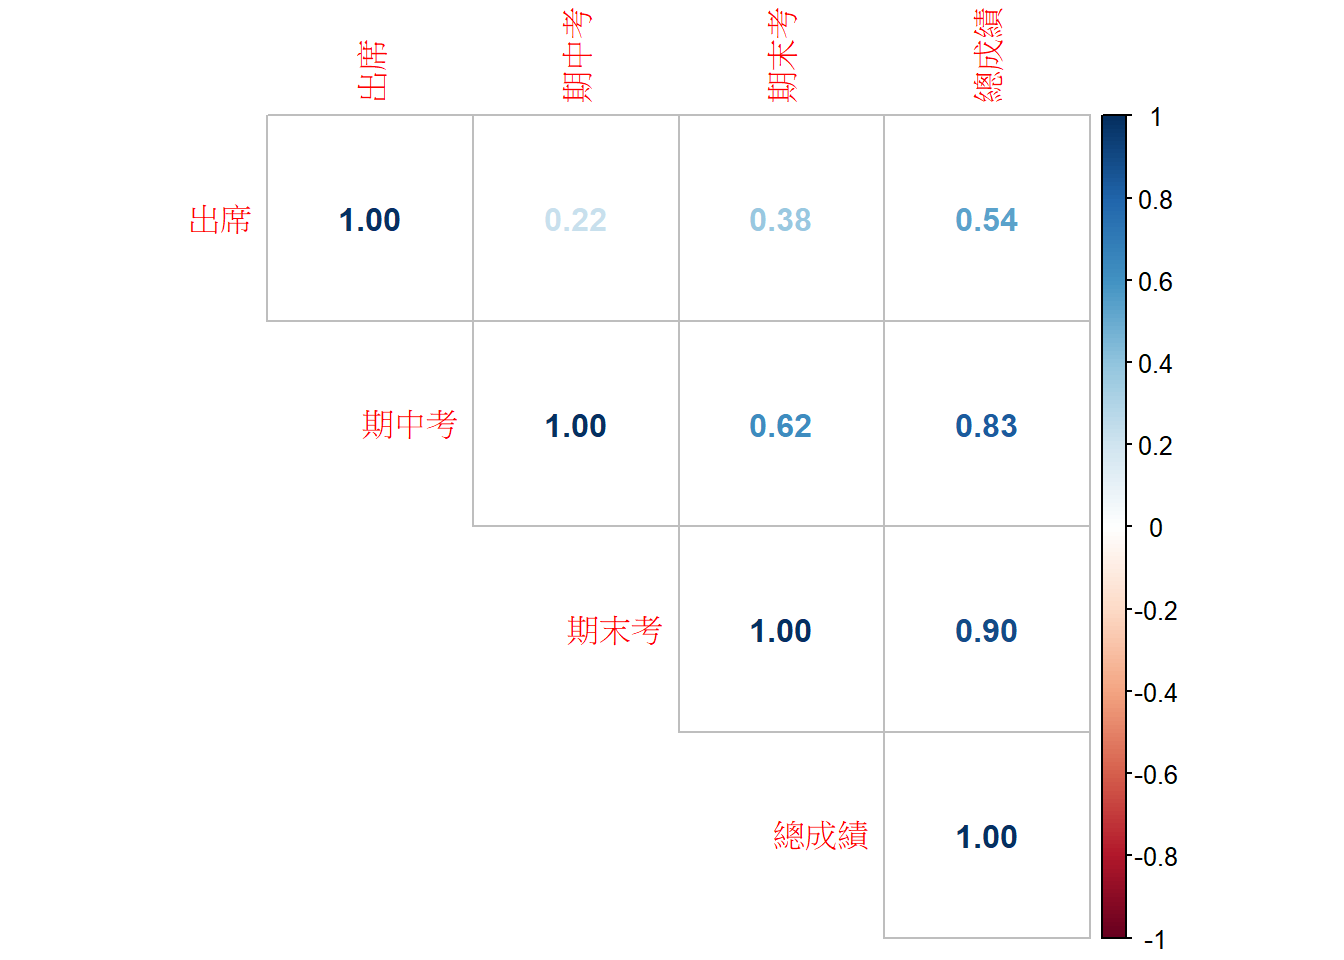
\includegraphics{quick-r-statistics_files/figure-latex/unnamed-chunk-48-1.pdf}

\begin{Shaded}
\begin{Highlighting}[]
\FunctionTok{corrplot}\NormalTok{(}\FunctionTok{cor}\NormalTok{(gData2), }\AttributeTok{method=}\StringTok{\textquotesingle{}color\textquotesingle{}}\NormalTok{, }\AttributeTok{type=}\StringTok{"upper"}\NormalTok{)}
\end{Highlighting}
\end{Shaded}

\begin{verbatim}
## Warning in strwidth(newrownames, cex = tl.cex): conversion failure on '出席' in
## 'mbcsToSbcs': dot substituted for <e5>
\end{verbatim}

\begin{verbatim}
## Warning in strwidth(newrownames, cex = tl.cex): conversion failure on '出席' in
## 'mbcsToSbcs': dot substituted for <87>
\end{verbatim}

\begin{verbatim}
## Warning in strwidth(newrownames, cex = tl.cex): conversion failure on '出席' in
## 'mbcsToSbcs': dot substituted for <ba>
\end{verbatim}

\begin{verbatim}
## Warning in strwidth(newrownames, cex = tl.cex): conversion failure on '出席' in
## 'mbcsToSbcs': dot substituted for <e5>
\end{verbatim}

\begin{verbatim}
## Warning in strwidth(newrownames, cex = tl.cex): conversion failure on '出席' in
## 'mbcsToSbcs': dot substituted for <b8>
\end{verbatim}

\begin{verbatim}
## Warning in strwidth(newrownames, cex = tl.cex): conversion failure on '出席' in
## 'mbcsToSbcs': dot substituted for <ad>
\end{verbatim}

\begin{verbatim}
## Warning in strwidth(newrownames, cex = tl.cex): conversion failure on '期中考'
## in 'mbcsToSbcs': dot substituted for <e6>
\end{verbatim}

\begin{verbatim}
## Warning in strwidth(newrownames, cex = tl.cex): conversion failure on '期中考'
## in 'mbcsToSbcs': dot substituted for <9c>
\end{verbatim}

\begin{verbatim}
## Warning in strwidth(newrownames, cex = tl.cex): conversion failure on '期中考'
## in 'mbcsToSbcs': dot substituted for <9f>
\end{verbatim}

\begin{verbatim}
## Warning in strwidth(newrownames, cex = tl.cex): conversion failure on '期中考'
## in 'mbcsToSbcs': dot substituted for <e4>
\end{verbatim}

\begin{verbatim}
## Warning in strwidth(newrownames, cex = tl.cex): conversion failure on '期中考'
## in 'mbcsToSbcs': dot substituted for <b8>
\end{verbatim}

\begin{verbatim}
## Warning in strwidth(newrownames, cex = tl.cex): conversion failure on '期中考'
## in 'mbcsToSbcs': dot substituted for <ad>
\end{verbatim}

\begin{verbatim}
## Warning in strwidth(newrownames, cex = tl.cex): conversion failure on '期中考'
## in 'mbcsToSbcs': dot substituted for <e8>
\end{verbatim}

\begin{verbatim}
## Warning in strwidth(newrownames, cex = tl.cex): conversion failure on '期中考'
## in 'mbcsToSbcs': dot substituted for <80>
\end{verbatim}

\begin{verbatim}
## Warning in strwidth(newrownames, cex = tl.cex): conversion failure on '期中考'
## in 'mbcsToSbcs': dot substituted for <83>
\end{verbatim}

\begin{verbatim}
## Warning in strwidth(newrownames, cex = tl.cex): conversion failure on '期末考'
## in 'mbcsToSbcs': dot substituted for <e6>
\end{verbatim}

\begin{verbatim}
## Warning in strwidth(newrownames, cex = tl.cex): conversion failure on '期末考'
## in 'mbcsToSbcs': dot substituted for <9c>
\end{verbatim}

\begin{verbatim}
## Warning in strwidth(newrownames, cex = tl.cex): conversion failure on '期末考'
## in 'mbcsToSbcs': dot substituted for <9f>
\end{verbatim}

\begin{verbatim}
## Warning in strwidth(newrownames, cex = tl.cex): conversion failure on '期末考'
## in 'mbcsToSbcs': dot substituted for <e6>
\end{verbatim}

\begin{verbatim}
## Warning in strwidth(newrownames, cex = tl.cex): conversion failure on '期末考'
## in 'mbcsToSbcs': dot substituted for <9c>
\end{verbatim}

\begin{verbatim}
## Warning in strwidth(newrownames, cex = tl.cex): conversion failure on '期末考'
## in 'mbcsToSbcs': dot substituted for <ab>
\end{verbatim}

\begin{verbatim}
## Warning in strwidth(newrownames, cex = tl.cex): conversion failure on '期末考'
## in 'mbcsToSbcs': dot substituted for <e8>
\end{verbatim}

\begin{verbatim}
## Warning in strwidth(newrownames, cex = tl.cex): conversion failure on '期末考'
## in 'mbcsToSbcs': dot substituted for <80>
\end{verbatim}

\begin{verbatim}
## Warning in strwidth(newrownames, cex = tl.cex): conversion failure on '期末考'
## in 'mbcsToSbcs': dot substituted for <83>
\end{verbatim}

\begin{verbatim}
## Warning in strwidth(newrownames, cex = tl.cex): conversion failure on '總成績'
## in 'mbcsToSbcs': dot substituted for <e7>
\end{verbatim}

\begin{verbatim}
## Warning in strwidth(newrownames, cex = tl.cex): conversion failure on '總成績'
## in 'mbcsToSbcs': dot substituted for <b8>
\end{verbatim}

\begin{verbatim}
## Warning in strwidth(newrownames, cex = tl.cex): conversion failure on '總成績'
## in 'mbcsToSbcs': dot substituted for <bd>
\end{verbatim}

\begin{verbatim}
## Warning in strwidth(newrownames, cex = tl.cex): conversion failure on '總成績'
## in 'mbcsToSbcs': dot substituted for <e6>
\end{verbatim}

\begin{verbatim}
## Warning in strwidth(newrownames, cex = tl.cex): conversion failure on '總成績'
## in 'mbcsToSbcs': dot substituted for <88>
\end{verbatim}

\begin{verbatim}
## Warning in strwidth(newrownames, cex = tl.cex): conversion failure on '總成績'
## in 'mbcsToSbcs': dot substituted for <90>
\end{verbatim}

\begin{verbatim}
## Warning in strwidth(newrownames, cex = tl.cex): conversion failure on '總成績'
## in 'mbcsToSbcs': dot substituted for <e7>
\end{verbatim}

\begin{verbatim}
## Warning in strwidth(newrownames, cex = tl.cex): conversion failure on '總成績'
## in 'mbcsToSbcs': dot substituted for <b8>
\end{verbatim}

\begin{verbatim}
## Warning in strwidth(newrownames, cex = tl.cex): conversion failure on '總成績'
## in 'mbcsToSbcs': dot substituted for <be>
\end{verbatim}

\begin{verbatim}
## Warning in strwidth(newcolnames, cex = tl.cex): conversion failure on '出席' in
## 'mbcsToSbcs': dot substituted for <e5>
\end{verbatim}

\begin{verbatim}
## Warning in strwidth(newcolnames, cex = tl.cex): conversion failure on '出席' in
## 'mbcsToSbcs': dot substituted for <87>
\end{verbatim}

\begin{verbatim}
## Warning in strwidth(newcolnames, cex = tl.cex): conversion failure on '出席' in
## 'mbcsToSbcs': dot substituted for <ba>
\end{verbatim}

\begin{verbatim}
## Warning in strwidth(newcolnames, cex = tl.cex): conversion failure on '出席' in
## 'mbcsToSbcs': dot substituted for <e5>
\end{verbatim}

\begin{verbatim}
## Warning in strwidth(newcolnames, cex = tl.cex): conversion failure on '出席' in
## 'mbcsToSbcs': dot substituted for <b8>
\end{verbatim}

\begin{verbatim}
## Warning in strwidth(newcolnames, cex = tl.cex): conversion failure on '出席' in
## 'mbcsToSbcs': dot substituted for <ad>
\end{verbatim}

\begin{verbatim}
## Warning in strwidth(newcolnames, cex = tl.cex): conversion failure on '期中考'
## in 'mbcsToSbcs': dot substituted for <e6>
\end{verbatim}

\begin{verbatim}
## Warning in strwidth(newcolnames, cex = tl.cex): conversion failure on '期中考'
## in 'mbcsToSbcs': dot substituted for <9c>
\end{verbatim}

\begin{verbatim}
## Warning in strwidth(newcolnames, cex = tl.cex): conversion failure on '期中考'
## in 'mbcsToSbcs': dot substituted for <9f>
\end{verbatim}

\begin{verbatim}
## Warning in strwidth(newcolnames, cex = tl.cex): conversion failure on '期中考'
## in 'mbcsToSbcs': dot substituted for <e4>
\end{verbatim}

\begin{verbatim}
## Warning in strwidth(newcolnames, cex = tl.cex): conversion failure on '期中考'
## in 'mbcsToSbcs': dot substituted for <b8>
\end{verbatim}

\begin{verbatim}
## Warning in strwidth(newcolnames, cex = tl.cex): conversion failure on '期中考'
## in 'mbcsToSbcs': dot substituted for <ad>
\end{verbatim}

\begin{verbatim}
## Warning in strwidth(newcolnames, cex = tl.cex): conversion failure on '期中考'
## in 'mbcsToSbcs': dot substituted for <e8>
\end{verbatim}

\begin{verbatim}
## Warning in strwidth(newcolnames, cex = tl.cex): conversion failure on '期中考'
## in 'mbcsToSbcs': dot substituted for <80>
\end{verbatim}

\begin{verbatim}
## Warning in strwidth(newcolnames, cex = tl.cex): conversion failure on '期中考'
## in 'mbcsToSbcs': dot substituted for <83>
\end{verbatim}

\begin{verbatim}
## Warning in strwidth(newcolnames, cex = tl.cex): conversion failure on '期末考'
## in 'mbcsToSbcs': dot substituted for <e6>
\end{verbatim}

\begin{verbatim}
## Warning in strwidth(newcolnames, cex = tl.cex): conversion failure on '期末考'
## in 'mbcsToSbcs': dot substituted for <9c>
\end{verbatim}

\begin{verbatim}
## Warning in strwidth(newcolnames, cex = tl.cex): conversion failure on '期末考'
## in 'mbcsToSbcs': dot substituted for <9f>
\end{verbatim}

\begin{verbatim}
## Warning in strwidth(newcolnames, cex = tl.cex): conversion failure on '期末考'
## in 'mbcsToSbcs': dot substituted for <e6>
\end{verbatim}

\begin{verbatim}
## Warning in strwidth(newcolnames, cex = tl.cex): conversion failure on '期末考'
## in 'mbcsToSbcs': dot substituted for <9c>
\end{verbatim}

\begin{verbatim}
## Warning in strwidth(newcolnames, cex = tl.cex): conversion failure on '期末考'
## in 'mbcsToSbcs': dot substituted for <ab>
\end{verbatim}

\begin{verbatim}
## Warning in strwidth(newcolnames, cex = tl.cex): conversion failure on '期末考'
## in 'mbcsToSbcs': dot substituted for <e8>
\end{verbatim}

\begin{verbatim}
## Warning in strwidth(newcolnames, cex = tl.cex): conversion failure on '期末考'
## in 'mbcsToSbcs': dot substituted for <80>
\end{verbatim}

\begin{verbatim}
## Warning in strwidth(newcolnames, cex = tl.cex): conversion failure on '期末考'
## in 'mbcsToSbcs': dot substituted for <83>
\end{verbatim}

\begin{verbatim}
## Warning in strwidth(newcolnames, cex = tl.cex): conversion failure on '總成績'
## in 'mbcsToSbcs': dot substituted for <e7>
\end{verbatim}

\begin{verbatim}
## Warning in strwidth(newcolnames, cex = tl.cex): conversion failure on '總成績'
## in 'mbcsToSbcs': dot substituted for <b8>
\end{verbatim}

\begin{verbatim}
## Warning in strwidth(newcolnames, cex = tl.cex): conversion failure on '總成績'
## in 'mbcsToSbcs': dot substituted for <bd>
\end{verbatim}

\begin{verbatim}
## Warning in strwidth(newcolnames, cex = tl.cex): conversion failure on '總成績'
## in 'mbcsToSbcs': dot substituted for <e6>
\end{verbatim}

\begin{verbatim}
## Warning in strwidth(newcolnames, cex = tl.cex): conversion failure on '總成績'
## in 'mbcsToSbcs': dot substituted for <88>
\end{verbatim}

\begin{verbatim}
## Warning in strwidth(newcolnames, cex = tl.cex): conversion failure on '總成績'
## in 'mbcsToSbcs': dot substituted for <90>
\end{verbatim}

\begin{verbatim}
## Warning in strwidth(newcolnames, cex = tl.cex): conversion failure on '總成績'
## in 'mbcsToSbcs': dot substituted for <e7>
\end{verbatim}

\begin{verbatim}
## Warning in strwidth(newcolnames, cex = tl.cex): conversion failure on '總成績'
## in 'mbcsToSbcs': dot substituted for <b8>
\end{verbatim}

\begin{verbatim}
## Warning in strwidth(newcolnames, cex = tl.cex): conversion failure on '總成績'
## in 'mbcsToSbcs': dot substituted for <be>
\end{verbatim}

\begin{verbatim}
## Warning in strwidth(newrownames, cex = tl.cex): conversion failure on '出席' in
## 'mbcsToSbcs': dot substituted for <e5>
\end{verbatim}

\begin{verbatim}
## Warning in strwidth(newrownames, cex = tl.cex): conversion failure on '出席' in
## 'mbcsToSbcs': dot substituted for <87>
\end{verbatim}

\begin{verbatim}
## Warning in strwidth(newrownames, cex = tl.cex): conversion failure on '出席' in
## 'mbcsToSbcs': dot substituted for <ba>
\end{verbatim}

\begin{verbatim}
## Warning in strwidth(newrownames, cex = tl.cex): conversion failure on '出席' in
## 'mbcsToSbcs': dot substituted for <e5>
\end{verbatim}

\begin{verbatim}
## Warning in strwidth(newrownames, cex = tl.cex): conversion failure on '出席' in
## 'mbcsToSbcs': dot substituted for <b8>
\end{verbatim}

\begin{verbatim}
## Warning in strwidth(newrownames, cex = tl.cex): conversion failure on '出席' in
## 'mbcsToSbcs': dot substituted for <ad>
\end{verbatim}

\begin{verbatim}
## Warning in strwidth(newrownames, cex = tl.cex): conversion failure on '期中考'
## in 'mbcsToSbcs': dot substituted for <e6>
\end{verbatim}

\begin{verbatim}
## Warning in strwidth(newrownames, cex = tl.cex): conversion failure on '期中考'
## in 'mbcsToSbcs': dot substituted for <9c>
\end{verbatim}

\begin{verbatim}
## Warning in strwidth(newrownames, cex = tl.cex): conversion failure on '期中考'
## in 'mbcsToSbcs': dot substituted for <9f>
\end{verbatim}

\begin{verbatim}
## Warning in strwidth(newrownames, cex = tl.cex): conversion failure on '期中考'
## in 'mbcsToSbcs': dot substituted for <e4>
\end{verbatim}

\begin{verbatim}
## Warning in strwidth(newrownames, cex = tl.cex): conversion failure on '期中考'
## in 'mbcsToSbcs': dot substituted for <b8>
\end{verbatim}

\begin{verbatim}
## Warning in strwidth(newrownames, cex = tl.cex): conversion failure on '期中考'
## in 'mbcsToSbcs': dot substituted for <ad>
\end{verbatim}

\begin{verbatim}
## Warning in strwidth(newrownames, cex = tl.cex): conversion failure on '期中考'
## in 'mbcsToSbcs': dot substituted for <e8>
\end{verbatim}

\begin{verbatim}
## Warning in strwidth(newrownames, cex = tl.cex): conversion failure on '期中考'
## in 'mbcsToSbcs': dot substituted for <80>
\end{verbatim}

\begin{verbatim}
## Warning in strwidth(newrownames, cex = tl.cex): conversion failure on '期中考'
## in 'mbcsToSbcs': dot substituted for <83>
\end{verbatim}

\begin{verbatim}
## Warning in strwidth(newrownames, cex = tl.cex): conversion failure on '期末考'
## in 'mbcsToSbcs': dot substituted for <e6>
\end{verbatim}

\begin{verbatim}
## Warning in strwidth(newrownames, cex = tl.cex): conversion failure on '期末考'
## in 'mbcsToSbcs': dot substituted for <9c>
\end{verbatim}

\begin{verbatim}
## Warning in strwidth(newrownames, cex = tl.cex): conversion failure on '期末考'
## in 'mbcsToSbcs': dot substituted for <9f>
\end{verbatim}

\begin{verbatim}
## Warning in strwidth(newrownames, cex = tl.cex): conversion failure on '期末考'
## in 'mbcsToSbcs': dot substituted for <e6>
\end{verbatim}

\begin{verbatim}
## Warning in strwidth(newrownames, cex = tl.cex): conversion failure on '期末考'
## in 'mbcsToSbcs': dot substituted for <9c>
\end{verbatim}

\begin{verbatim}
## Warning in strwidth(newrownames, cex = tl.cex): conversion failure on '期末考'
## in 'mbcsToSbcs': dot substituted for <ab>
\end{verbatim}

\begin{verbatim}
## Warning in strwidth(newrownames, cex = tl.cex): conversion failure on '期末考'
## in 'mbcsToSbcs': dot substituted for <e8>
\end{verbatim}

\begin{verbatim}
## Warning in strwidth(newrownames, cex = tl.cex): conversion failure on '期末考'
## in 'mbcsToSbcs': dot substituted for <80>
\end{verbatim}

\begin{verbatim}
## Warning in strwidth(newrownames, cex = tl.cex): conversion failure on '期末考'
## in 'mbcsToSbcs': dot substituted for <83>
\end{verbatim}

\begin{verbatim}
## Warning in strwidth(newrownames, cex = tl.cex): conversion failure on '總成績'
## in 'mbcsToSbcs': dot substituted for <e7>
\end{verbatim}

\begin{verbatim}
## Warning in strwidth(newrownames, cex = tl.cex): conversion failure on '總成績'
## in 'mbcsToSbcs': dot substituted for <b8>
\end{verbatim}

\begin{verbatim}
## Warning in strwidth(newrownames, cex = tl.cex): conversion failure on '總成績'
## in 'mbcsToSbcs': dot substituted for <bd>
\end{verbatim}

\begin{verbatim}
## Warning in strwidth(newrownames, cex = tl.cex): conversion failure on '總成績'
## in 'mbcsToSbcs': dot substituted for <e6>
\end{verbatim}

\begin{verbatim}
## Warning in strwidth(newrownames, cex = tl.cex): conversion failure on '總成績'
## in 'mbcsToSbcs': dot substituted for <88>
\end{verbatim}

\begin{verbatim}
## Warning in strwidth(newrownames, cex = tl.cex): conversion failure on '總成績'
## in 'mbcsToSbcs': dot substituted for <90>
\end{verbatim}

\begin{verbatim}
## Warning in strwidth(newrownames, cex = tl.cex): conversion failure on '總成績'
## in 'mbcsToSbcs': dot substituted for <e7>
\end{verbatim}

\begin{verbatim}
## Warning in strwidth(newrownames, cex = tl.cex): conversion failure on '總成績'
## in 'mbcsToSbcs': dot substituted for <b8>
\end{verbatim}

\begin{verbatim}
## Warning in strwidth(newrownames, cex = tl.cex): conversion failure on '總成績'
## in 'mbcsToSbcs': dot substituted for <be>
\end{verbatim}

\begin{verbatim}
## Warning in strwidth(newcolnames, cex = tl.cex): conversion failure on '出席' in
## 'mbcsToSbcs': dot substituted for <e5>
\end{verbatim}

\begin{verbatim}
## Warning in strwidth(newcolnames, cex = tl.cex): conversion failure on '出席' in
## 'mbcsToSbcs': dot substituted for <87>
\end{verbatim}

\begin{verbatim}
## Warning in strwidth(newcolnames, cex = tl.cex): conversion failure on '出席' in
## 'mbcsToSbcs': dot substituted for <ba>
\end{verbatim}

\begin{verbatim}
## Warning in strwidth(newcolnames, cex = tl.cex): conversion failure on '出席' in
## 'mbcsToSbcs': dot substituted for <e5>
\end{verbatim}

\begin{verbatim}
## Warning in strwidth(newcolnames, cex = tl.cex): conversion failure on '出席' in
## 'mbcsToSbcs': dot substituted for <b8>
\end{verbatim}

\begin{verbatim}
## Warning in strwidth(newcolnames, cex = tl.cex): conversion failure on '出席' in
## 'mbcsToSbcs': dot substituted for <ad>
\end{verbatim}

\begin{verbatim}
## Warning in strwidth(newcolnames, cex = tl.cex): conversion failure on '期中考'
## in 'mbcsToSbcs': dot substituted for <e6>
\end{verbatim}

\begin{verbatim}
## Warning in strwidth(newcolnames, cex = tl.cex): conversion failure on '期中考'
## in 'mbcsToSbcs': dot substituted for <9c>
\end{verbatim}

\begin{verbatim}
## Warning in strwidth(newcolnames, cex = tl.cex): conversion failure on '期中考'
## in 'mbcsToSbcs': dot substituted for <9f>
\end{verbatim}

\begin{verbatim}
## Warning in strwidth(newcolnames, cex = tl.cex): conversion failure on '期中考'
## in 'mbcsToSbcs': dot substituted for <e4>
\end{verbatim}

\begin{verbatim}
## Warning in strwidth(newcolnames, cex = tl.cex): conversion failure on '期中考'
## in 'mbcsToSbcs': dot substituted for <b8>
\end{verbatim}

\begin{verbatim}
## Warning in strwidth(newcolnames, cex = tl.cex): conversion failure on '期中考'
## in 'mbcsToSbcs': dot substituted for <ad>
\end{verbatim}

\begin{verbatim}
## Warning in strwidth(newcolnames, cex = tl.cex): conversion failure on '期中考'
## in 'mbcsToSbcs': dot substituted for <e8>
\end{verbatim}

\begin{verbatim}
## Warning in strwidth(newcolnames, cex = tl.cex): conversion failure on '期中考'
## in 'mbcsToSbcs': dot substituted for <80>
\end{verbatim}

\begin{verbatim}
## Warning in strwidth(newcolnames, cex = tl.cex): conversion failure on '期中考'
## in 'mbcsToSbcs': dot substituted for <83>
\end{verbatim}

\begin{verbatim}
## Warning in strwidth(newcolnames, cex = tl.cex): conversion failure on '期末考'
## in 'mbcsToSbcs': dot substituted for <e6>
\end{verbatim}

\begin{verbatim}
## Warning in strwidth(newcolnames, cex = tl.cex): conversion failure on '期末考'
## in 'mbcsToSbcs': dot substituted for <9c>
\end{verbatim}

\begin{verbatim}
## Warning in strwidth(newcolnames, cex = tl.cex): conversion failure on '期末考'
## in 'mbcsToSbcs': dot substituted for <9f>
\end{verbatim}

\begin{verbatim}
## Warning in strwidth(newcolnames, cex = tl.cex): conversion failure on '期末考'
## in 'mbcsToSbcs': dot substituted for <e6>
\end{verbatim}

\begin{verbatim}
## Warning in strwidth(newcolnames, cex = tl.cex): conversion failure on '期末考'
## in 'mbcsToSbcs': dot substituted for <9c>
\end{verbatim}

\begin{verbatim}
## Warning in strwidth(newcolnames, cex = tl.cex): conversion failure on '期末考'
## in 'mbcsToSbcs': dot substituted for <ab>
\end{verbatim}

\begin{verbatim}
## Warning in strwidth(newcolnames, cex = tl.cex): conversion failure on '期末考'
## in 'mbcsToSbcs': dot substituted for <e8>
\end{verbatim}

\begin{verbatim}
## Warning in strwidth(newcolnames, cex = tl.cex): conversion failure on '期末考'
## in 'mbcsToSbcs': dot substituted for <80>
\end{verbatim}

\begin{verbatim}
## Warning in strwidth(newcolnames, cex = tl.cex): conversion failure on '期末考'
## in 'mbcsToSbcs': dot substituted for <83>
\end{verbatim}

\begin{verbatim}
## Warning in strwidth(newcolnames, cex = tl.cex): conversion failure on '總成績'
## in 'mbcsToSbcs': dot substituted for <e7>
\end{verbatim}

\begin{verbatim}
## Warning in strwidth(newcolnames, cex = tl.cex): conversion failure on '總成績'
## in 'mbcsToSbcs': dot substituted for <b8>
\end{verbatim}

\begin{verbatim}
## Warning in strwidth(newcolnames, cex = tl.cex): conversion failure on '總成績'
## in 'mbcsToSbcs': dot substituted for <bd>
\end{verbatim}

\begin{verbatim}
## Warning in strwidth(newcolnames, cex = tl.cex): conversion failure on '總成績'
## in 'mbcsToSbcs': dot substituted for <e6>
\end{verbatim}

\begin{verbatim}
## Warning in strwidth(newcolnames, cex = tl.cex): conversion failure on '總成績'
## in 'mbcsToSbcs': dot substituted for <88>
\end{verbatim}

\begin{verbatim}
## Warning in strwidth(newcolnames, cex = tl.cex): conversion failure on '總成績'
## in 'mbcsToSbcs': dot substituted for <90>
\end{verbatim}

\begin{verbatim}
## Warning in strwidth(newcolnames, cex = tl.cex): conversion failure on '總成績'
## in 'mbcsToSbcs': dot substituted for <e7>
\end{verbatim}

\begin{verbatim}
## Warning in strwidth(newcolnames, cex = tl.cex): conversion failure on '總成績'
## in 'mbcsToSbcs': dot substituted for <b8>
\end{verbatim}

\begin{verbatim}
## Warning in strwidth(newcolnames, cex = tl.cex): conversion failure on '總成績'
## in 'mbcsToSbcs': dot substituted for <be>
\end{verbatim}

\begin{verbatim}
## Warning in strwidth(newrownames, cex = tl.cex): conversion failure on '出席' in
## 'mbcsToSbcs': dot substituted for <e5>
\end{verbatim}

\begin{verbatim}
## Warning in strwidth(newrownames, cex = tl.cex): conversion failure on '出席' in
## 'mbcsToSbcs': dot substituted for <87>
\end{verbatim}

\begin{verbatim}
## Warning in strwidth(newrownames, cex = tl.cex): conversion failure on '出席' in
## 'mbcsToSbcs': dot substituted for <ba>
\end{verbatim}

\begin{verbatim}
## Warning in strwidth(newrownames, cex = tl.cex): conversion failure on '出席' in
## 'mbcsToSbcs': dot substituted for <e5>
\end{verbatim}

\begin{verbatim}
## Warning in strwidth(newrownames, cex = tl.cex): conversion failure on '出席' in
## 'mbcsToSbcs': dot substituted for <b8>
\end{verbatim}

\begin{verbatim}
## Warning in strwidth(newrownames, cex = tl.cex): conversion failure on '出席' in
## 'mbcsToSbcs': dot substituted for <ad>
\end{verbatim}

\begin{verbatim}
## Warning in strwidth(newrownames, cex = tl.cex): conversion failure on '期中考'
## in 'mbcsToSbcs': dot substituted for <e6>
\end{verbatim}

\begin{verbatim}
## Warning in strwidth(newrownames, cex = tl.cex): conversion failure on '期中考'
## in 'mbcsToSbcs': dot substituted for <9c>
\end{verbatim}

\begin{verbatim}
## Warning in strwidth(newrownames, cex = tl.cex): conversion failure on '期中考'
## in 'mbcsToSbcs': dot substituted for <9f>
\end{verbatim}

\begin{verbatim}
## Warning in strwidth(newrownames, cex = tl.cex): conversion failure on '期中考'
## in 'mbcsToSbcs': dot substituted for <e4>
\end{verbatim}

\begin{verbatim}
## Warning in strwidth(newrownames, cex = tl.cex): conversion failure on '期中考'
## in 'mbcsToSbcs': dot substituted for <b8>
\end{verbatim}

\begin{verbatim}
## Warning in strwidth(newrownames, cex = tl.cex): conversion failure on '期中考'
## in 'mbcsToSbcs': dot substituted for <ad>
\end{verbatim}

\begin{verbatim}
## Warning in strwidth(newrownames, cex = tl.cex): conversion failure on '期中考'
## in 'mbcsToSbcs': dot substituted for <e8>
\end{verbatim}

\begin{verbatim}
## Warning in strwidth(newrownames, cex = tl.cex): conversion failure on '期中考'
## in 'mbcsToSbcs': dot substituted for <80>
\end{verbatim}

\begin{verbatim}
## Warning in strwidth(newrownames, cex = tl.cex): conversion failure on '期中考'
## in 'mbcsToSbcs': dot substituted for <83>
\end{verbatim}

\begin{verbatim}
## Warning in strwidth(newrownames, cex = tl.cex): conversion failure on '期末考'
## in 'mbcsToSbcs': dot substituted for <e6>
\end{verbatim}

\begin{verbatim}
## Warning in strwidth(newrownames, cex = tl.cex): conversion failure on '期末考'
## in 'mbcsToSbcs': dot substituted for <9c>
\end{verbatim}

\begin{verbatim}
## Warning in strwidth(newrownames, cex = tl.cex): conversion failure on '期末考'
## in 'mbcsToSbcs': dot substituted for <9f>
\end{verbatim}

\begin{verbatim}
## Warning in strwidth(newrownames, cex = tl.cex): conversion failure on '期末考'
## in 'mbcsToSbcs': dot substituted for <e6>
\end{verbatim}

\begin{verbatim}
## Warning in strwidth(newrownames, cex = tl.cex): conversion failure on '期末考'
## in 'mbcsToSbcs': dot substituted for <9c>
\end{verbatim}

\begin{verbatim}
## Warning in strwidth(newrownames, cex = tl.cex): conversion failure on '期末考'
## in 'mbcsToSbcs': dot substituted for <ab>
\end{verbatim}

\begin{verbatim}
## Warning in strwidth(newrownames, cex = tl.cex): conversion failure on '期末考'
## in 'mbcsToSbcs': dot substituted for <e8>
\end{verbatim}

\begin{verbatim}
## Warning in strwidth(newrownames, cex = tl.cex): conversion failure on '期末考'
## in 'mbcsToSbcs': dot substituted for <80>
\end{verbatim}

\begin{verbatim}
## Warning in strwidth(newrownames, cex = tl.cex): conversion failure on '期末考'
## in 'mbcsToSbcs': dot substituted for <83>
\end{verbatim}

\begin{verbatim}
## Warning in strwidth(newrownames, cex = tl.cex): conversion failure on '總成績'
## in 'mbcsToSbcs': dot substituted for <e7>
\end{verbatim}

\begin{verbatim}
## Warning in strwidth(newrownames, cex = tl.cex): conversion failure on '總成績'
## in 'mbcsToSbcs': dot substituted for <b8>
\end{verbatim}

\begin{verbatim}
## Warning in strwidth(newrownames, cex = tl.cex): conversion failure on '總成績'
## in 'mbcsToSbcs': dot substituted for <bd>
\end{verbatim}

\begin{verbatim}
## Warning in strwidth(newrownames, cex = tl.cex): conversion failure on '總成績'
## in 'mbcsToSbcs': dot substituted for <e6>
\end{verbatim}

\begin{verbatim}
## Warning in strwidth(newrownames, cex = tl.cex): conversion failure on '總成績'
## in 'mbcsToSbcs': dot substituted for <88>
\end{verbatim}

\begin{verbatim}
## Warning in strwidth(newrownames, cex = tl.cex): conversion failure on '總成績'
## in 'mbcsToSbcs': dot substituted for <90>
\end{verbatim}

\begin{verbatim}
## Warning in strwidth(newrownames, cex = tl.cex): conversion failure on '總成績'
## in 'mbcsToSbcs': dot substituted for <e7>
\end{verbatim}

\begin{verbatim}
## Warning in strwidth(newrownames, cex = tl.cex): conversion failure on '總成績'
## in 'mbcsToSbcs': dot substituted for <b8>
\end{verbatim}

\begin{verbatim}
## Warning in strwidth(newrownames, cex = tl.cex): conversion failure on '總成績'
## in 'mbcsToSbcs': dot substituted for <be>
\end{verbatim}

\begin{verbatim}
## Warning in strwidth(newcolnames, cex = tl.cex): conversion failure on '出席' in
## 'mbcsToSbcs': dot substituted for <e5>
\end{verbatim}

\begin{verbatim}
## Warning in strwidth(newcolnames, cex = tl.cex): conversion failure on '出席' in
## 'mbcsToSbcs': dot substituted for <87>
\end{verbatim}

\begin{verbatim}
## Warning in strwidth(newcolnames, cex = tl.cex): conversion failure on '出席' in
## 'mbcsToSbcs': dot substituted for <ba>
\end{verbatim}

\begin{verbatim}
## Warning in strwidth(newcolnames, cex = tl.cex): conversion failure on '出席' in
## 'mbcsToSbcs': dot substituted for <e5>
\end{verbatim}

\begin{verbatim}
## Warning in strwidth(newcolnames, cex = tl.cex): conversion failure on '出席' in
## 'mbcsToSbcs': dot substituted for <b8>
\end{verbatim}

\begin{verbatim}
## Warning in strwidth(newcolnames, cex = tl.cex): conversion failure on '出席' in
## 'mbcsToSbcs': dot substituted for <ad>
\end{verbatim}

\begin{verbatim}
## Warning in strwidth(newcolnames, cex = tl.cex): conversion failure on '期中考'
## in 'mbcsToSbcs': dot substituted for <e6>
\end{verbatim}

\begin{verbatim}
## Warning in strwidth(newcolnames, cex = tl.cex): conversion failure on '期中考'
## in 'mbcsToSbcs': dot substituted for <9c>
\end{verbatim}

\begin{verbatim}
## Warning in strwidth(newcolnames, cex = tl.cex): conversion failure on '期中考'
## in 'mbcsToSbcs': dot substituted for <9f>
\end{verbatim}

\begin{verbatim}
## Warning in strwidth(newcolnames, cex = tl.cex): conversion failure on '期中考'
## in 'mbcsToSbcs': dot substituted for <e4>
\end{verbatim}

\begin{verbatim}
## Warning in strwidth(newcolnames, cex = tl.cex): conversion failure on '期中考'
## in 'mbcsToSbcs': dot substituted for <b8>
\end{verbatim}

\begin{verbatim}
## Warning in strwidth(newcolnames, cex = tl.cex): conversion failure on '期中考'
## in 'mbcsToSbcs': dot substituted for <ad>
\end{verbatim}

\begin{verbatim}
## Warning in strwidth(newcolnames, cex = tl.cex): conversion failure on '期中考'
## in 'mbcsToSbcs': dot substituted for <e8>
\end{verbatim}

\begin{verbatim}
## Warning in strwidth(newcolnames, cex = tl.cex): conversion failure on '期中考'
## in 'mbcsToSbcs': dot substituted for <80>
\end{verbatim}

\begin{verbatim}
## Warning in strwidth(newcolnames, cex = tl.cex): conversion failure on '期中考'
## in 'mbcsToSbcs': dot substituted for <83>
\end{verbatim}

\begin{verbatim}
## Warning in strwidth(newcolnames, cex = tl.cex): conversion failure on '期末考'
## in 'mbcsToSbcs': dot substituted for <e6>
\end{verbatim}

\begin{verbatim}
## Warning in strwidth(newcolnames, cex = tl.cex): conversion failure on '期末考'
## in 'mbcsToSbcs': dot substituted for <9c>
\end{verbatim}

\begin{verbatim}
## Warning in strwidth(newcolnames, cex = tl.cex): conversion failure on '期末考'
## in 'mbcsToSbcs': dot substituted for <9f>
\end{verbatim}

\begin{verbatim}
## Warning in strwidth(newcolnames, cex = tl.cex): conversion failure on '期末考'
## in 'mbcsToSbcs': dot substituted for <e6>
\end{verbatim}

\begin{verbatim}
## Warning in strwidth(newcolnames, cex = tl.cex): conversion failure on '期末考'
## in 'mbcsToSbcs': dot substituted for <9c>
\end{verbatim}

\begin{verbatim}
## Warning in strwidth(newcolnames, cex = tl.cex): conversion failure on '期末考'
## in 'mbcsToSbcs': dot substituted for <ab>
\end{verbatim}

\begin{verbatim}
## Warning in strwidth(newcolnames, cex = tl.cex): conversion failure on '期末考'
## in 'mbcsToSbcs': dot substituted for <e8>
\end{verbatim}

\begin{verbatim}
## Warning in strwidth(newcolnames, cex = tl.cex): conversion failure on '期末考'
## in 'mbcsToSbcs': dot substituted for <80>
\end{verbatim}

\begin{verbatim}
## Warning in strwidth(newcolnames, cex = tl.cex): conversion failure on '期末考'
## in 'mbcsToSbcs': dot substituted for <83>
\end{verbatim}

\begin{verbatim}
## Warning in strwidth(newcolnames, cex = tl.cex): conversion failure on '總成績'
## in 'mbcsToSbcs': dot substituted for <e7>
\end{verbatim}

\begin{verbatim}
## Warning in strwidth(newcolnames, cex = tl.cex): conversion failure on '總成績'
## in 'mbcsToSbcs': dot substituted for <b8>
\end{verbatim}

\begin{verbatim}
## Warning in strwidth(newcolnames, cex = tl.cex): conversion failure on '總成績'
## in 'mbcsToSbcs': dot substituted for <bd>
\end{verbatim}

\begin{verbatim}
## Warning in strwidth(newcolnames, cex = tl.cex): conversion failure on '總成績'
## in 'mbcsToSbcs': dot substituted for <e6>
\end{verbatim}

\begin{verbatim}
## Warning in strwidth(newcolnames, cex = tl.cex): conversion failure on '總成績'
## in 'mbcsToSbcs': dot substituted for <88>
\end{verbatim}

\begin{verbatim}
## Warning in strwidth(newcolnames, cex = tl.cex): conversion failure on '總成績'
## in 'mbcsToSbcs': dot substituted for <90>
\end{verbatim}

\begin{verbatim}
## Warning in strwidth(newcolnames, cex = tl.cex): conversion failure on '總成績'
## in 'mbcsToSbcs': dot substituted for <e7>
\end{verbatim}

\begin{verbatim}
## Warning in strwidth(newcolnames, cex = tl.cex): conversion failure on '總成績'
## in 'mbcsToSbcs': dot substituted for <b8>
\end{verbatim}

\begin{verbatim}
## Warning in strwidth(newcolnames, cex = tl.cex): conversion failure on '總成績'
## in 'mbcsToSbcs': dot substituted for <be>
\end{verbatim}

\begin{verbatim}
## Warning in strwidth(newrownames, cex = tl.cex): conversion failure on '出席' in
## 'mbcsToSbcs': dot substituted for <e5>
\end{verbatim}

\begin{verbatim}
## Warning in strwidth(newrownames, cex = tl.cex): conversion failure on '出席' in
## 'mbcsToSbcs': dot substituted for <87>
\end{verbatim}

\begin{verbatim}
## Warning in strwidth(newrownames, cex = tl.cex): conversion failure on '出席' in
## 'mbcsToSbcs': dot substituted for <ba>
\end{verbatim}

\begin{verbatim}
## Warning in strwidth(newrownames, cex = tl.cex): conversion failure on '出席' in
## 'mbcsToSbcs': dot substituted for <e5>
\end{verbatim}

\begin{verbatim}
## Warning in strwidth(newrownames, cex = tl.cex): conversion failure on '出席' in
## 'mbcsToSbcs': dot substituted for <b8>
\end{verbatim}

\begin{verbatim}
## Warning in strwidth(newrownames, cex = tl.cex): conversion failure on '出席' in
## 'mbcsToSbcs': dot substituted for <ad>
\end{verbatim}

\begin{verbatim}
## Warning in strwidth(newrownames, cex = tl.cex): conversion failure on '期中考'
## in 'mbcsToSbcs': dot substituted for <e6>
\end{verbatim}

\begin{verbatim}
## Warning in strwidth(newrownames, cex = tl.cex): conversion failure on '期中考'
## in 'mbcsToSbcs': dot substituted for <9c>
\end{verbatim}

\begin{verbatim}
## Warning in strwidth(newrownames, cex = tl.cex): conversion failure on '期中考'
## in 'mbcsToSbcs': dot substituted for <9f>
\end{verbatim}

\begin{verbatim}
## Warning in strwidth(newrownames, cex = tl.cex): conversion failure on '期中考'
## in 'mbcsToSbcs': dot substituted for <e4>
\end{verbatim}

\begin{verbatim}
## Warning in strwidth(newrownames, cex = tl.cex): conversion failure on '期中考'
## in 'mbcsToSbcs': dot substituted for <b8>
\end{verbatim}

\begin{verbatim}
## Warning in strwidth(newrownames, cex = tl.cex): conversion failure on '期中考'
## in 'mbcsToSbcs': dot substituted for <ad>
\end{verbatim}

\begin{verbatim}
## Warning in strwidth(newrownames, cex = tl.cex): conversion failure on '期中考'
## in 'mbcsToSbcs': dot substituted for <e8>
\end{verbatim}

\begin{verbatim}
## Warning in strwidth(newrownames, cex = tl.cex): conversion failure on '期中考'
## in 'mbcsToSbcs': dot substituted for <80>
\end{verbatim}

\begin{verbatim}
## Warning in strwidth(newrownames, cex = tl.cex): conversion failure on '期中考'
## in 'mbcsToSbcs': dot substituted for <83>
\end{verbatim}

\begin{verbatim}
## Warning in strwidth(newrownames, cex = tl.cex): conversion failure on '期末考'
## in 'mbcsToSbcs': dot substituted for <e6>
\end{verbatim}

\begin{verbatim}
## Warning in strwidth(newrownames, cex = tl.cex): conversion failure on '期末考'
## in 'mbcsToSbcs': dot substituted for <9c>
\end{verbatim}

\begin{verbatim}
## Warning in strwidth(newrownames, cex = tl.cex): conversion failure on '期末考'
## in 'mbcsToSbcs': dot substituted for <9f>
\end{verbatim}

\begin{verbatim}
## Warning in strwidth(newrownames, cex = tl.cex): conversion failure on '期末考'
## in 'mbcsToSbcs': dot substituted for <e6>
\end{verbatim}

\begin{verbatim}
## Warning in strwidth(newrownames, cex = tl.cex): conversion failure on '期末考'
## in 'mbcsToSbcs': dot substituted for <9c>
\end{verbatim}

\begin{verbatim}
## Warning in strwidth(newrownames, cex = tl.cex): conversion failure on '期末考'
## in 'mbcsToSbcs': dot substituted for <ab>
\end{verbatim}

\begin{verbatim}
## Warning in strwidth(newrownames, cex = tl.cex): conversion failure on '期末考'
## in 'mbcsToSbcs': dot substituted for <e8>
\end{verbatim}

\begin{verbatim}
## Warning in strwidth(newrownames, cex = tl.cex): conversion failure on '期末考'
## in 'mbcsToSbcs': dot substituted for <80>
\end{verbatim}

\begin{verbatim}
## Warning in strwidth(newrownames, cex = tl.cex): conversion failure on '期末考'
## in 'mbcsToSbcs': dot substituted for <83>
\end{verbatim}

\begin{verbatim}
## Warning in strwidth(newrownames, cex = tl.cex): conversion failure on '總成績'
## in 'mbcsToSbcs': dot substituted for <e7>
\end{verbatim}

\begin{verbatim}
## Warning in strwidth(newrownames, cex = tl.cex): conversion failure on '總成績'
## in 'mbcsToSbcs': dot substituted for <b8>
\end{verbatim}

\begin{verbatim}
## Warning in strwidth(newrownames, cex = tl.cex): conversion failure on '總成績'
## in 'mbcsToSbcs': dot substituted for <bd>
\end{verbatim}

\begin{verbatim}
## Warning in strwidth(newrownames, cex = tl.cex): conversion failure on '總成績'
## in 'mbcsToSbcs': dot substituted for <e6>
\end{verbatim}

\begin{verbatim}
## Warning in strwidth(newrownames, cex = tl.cex): conversion failure on '總成績'
## in 'mbcsToSbcs': dot substituted for <88>
\end{verbatim}

\begin{verbatim}
## Warning in strwidth(newrownames, cex = tl.cex): conversion failure on '總成績'
## in 'mbcsToSbcs': dot substituted for <90>
\end{verbatim}

\begin{verbatim}
## Warning in strwidth(newrownames, cex = tl.cex): conversion failure on '總成績'
## in 'mbcsToSbcs': dot substituted for <e7>
\end{verbatim}

\begin{verbatim}
## Warning in strwidth(newrownames, cex = tl.cex): conversion failure on '總成績'
## in 'mbcsToSbcs': dot substituted for <b8>
\end{verbatim}

\begin{verbatim}
## Warning in strwidth(newrownames, cex = tl.cex): conversion failure on '總成績'
## in 'mbcsToSbcs': dot substituted for <be>
\end{verbatim}

\begin{verbatim}
## Warning in strwidth(newcolnames, cex = tl.cex): conversion failure on '出席' in
## 'mbcsToSbcs': dot substituted for <e5>
\end{verbatim}

\begin{verbatim}
## Warning in strwidth(newcolnames, cex = tl.cex): conversion failure on '出席' in
## 'mbcsToSbcs': dot substituted for <87>
\end{verbatim}

\begin{verbatim}
## Warning in strwidth(newcolnames, cex = tl.cex): conversion failure on '出席' in
## 'mbcsToSbcs': dot substituted for <ba>
\end{verbatim}

\begin{verbatim}
## Warning in strwidth(newcolnames, cex = tl.cex): conversion failure on '出席' in
## 'mbcsToSbcs': dot substituted for <e5>
\end{verbatim}

\begin{verbatim}
## Warning in strwidth(newcolnames, cex = tl.cex): conversion failure on '出席' in
## 'mbcsToSbcs': dot substituted for <b8>
\end{verbatim}

\begin{verbatim}
## Warning in strwidth(newcolnames, cex = tl.cex): conversion failure on '出席' in
## 'mbcsToSbcs': dot substituted for <ad>
\end{verbatim}

\begin{verbatim}
## Warning in strwidth(newcolnames, cex = tl.cex): conversion failure on '期中考'
## in 'mbcsToSbcs': dot substituted for <e6>
\end{verbatim}

\begin{verbatim}
## Warning in strwidth(newcolnames, cex = tl.cex): conversion failure on '期中考'
## in 'mbcsToSbcs': dot substituted for <9c>
\end{verbatim}

\begin{verbatim}
## Warning in strwidth(newcolnames, cex = tl.cex): conversion failure on '期中考'
## in 'mbcsToSbcs': dot substituted for <9f>
\end{verbatim}

\begin{verbatim}
## Warning in strwidth(newcolnames, cex = tl.cex): conversion failure on '期中考'
## in 'mbcsToSbcs': dot substituted for <e4>
\end{verbatim}

\begin{verbatim}
## Warning in strwidth(newcolnames, cex = tl.cex): conversion failure on '期中考'
## in 'mbcsToSbcs': dot substituted for <b8>
\end{verbatim}

\begin{verbatim}
## Warning in strwidth(newcolnames, cex = tl.cex): conversion failure on '期中考'
## in 'mbcsToSbcs': dot substituted for <ad>
\end{verbatim}

\begin{verbatim}
## Warning in strwidth(newcolnames, cex = tl.cex): conversion failure on '期中考'
## in 'mbcsToSbcs': dot substituted for <e8>
\end{verbatim}

\begin{verbatim}
## Warning in strwidth(newcolnames, cex = tl.cex): conversion failure on '期中考'
## in 'mbcsToSbcs': dot substituted for <80>
\end{verbatim}

\begin{verbatim}
## Warning in strwidth(newcolnames, cex = tl.cex): conversion failure on '期中考'
## in 'mbcsToSbcs': dot substituted for <83>
\end{verbatim}

\begin{verbatim}
## Warning in strwidth(newcolnames, cex = tl.cex): conversion failure on '期末考'
## in 'mbcsToSbcs': dot substituted for <e6>
\end{verbatim}

\begin{verbatim}
## Warning in strwidth(newcolnames, cex = tl.cex): conversion failure on '期末考'
## in 'mbcsToSbcs': dot substituted for <9c>
\end{verbatim}

\begin{verbatim}
## Warning in strwidth(newcolnames, cex = tl.cex): conversion failure on '期末考'
## in 'mbcsToSbcs': dot substituted for <9f>
\end{verbatim}

\begin{verbatim}
## Warning in strwidth(newcolnames, cex = tl.cex): conversion failure on '期末考'
## in 'mbcsToSbcs': dot substituted for <e6>
\end{verbatim}

\begin{verbatim}
## Warning in strwidth(newcolnames, cex = tl.cex): conversion failure on '期末考'
## in 'mbcsToSbcs': dot substituted for <9c>
\end{verbatim}

\begin{verbatim}
## Warning in strwidth(newcolnames, cex = tl.cex): conversion failure on '期末考'
## in 'mbcsToSbcs': dot substituted for <ab>
\end{verbatim}

\begin{verbatim}
## Warning in strwidth(newcolnames, cex = tl.cex): conversion failure on '期末考'
## in 'mbcsToSbcs': dot substituted for <e8>
\end{verbatim}

\begin{verbatim}
## Warning in strwidth(newcolnames, cex = tl.cex): conversion failure on '期末考'
## in 'mbcsToSbcs': dot substituted for <80>
\end{verbatim}

\begin{verbatim}
## Warning in strwidth(newcolnames, cex = tl.cex): conversion failure on '期末考'
## in 'mbcsToSbcs': dot substituted for <83>
\end{verbatim}

\begin{verbatim}
## Warning in strwidth(newcolnames, cex = tl.cex): conversion failure on '總成績'
## in 'mbcsToSbcs': dot substituted for <e7>
\end{verbatim}

\begin{verbatim}
## Warning in strwidth(newcolnames, cex = tl.cex): conversion failure on '總成績'
## in 'mbcsToSbcs': dot substituted for <b8>
\end{verbatim}

\begin{verbatim}
## Warning in strwidth(newcolnames, cex = tl.cex): conversion failure on '總成績'
## in 'mbcsToSbcs': dot substituted for <bd>
\end{verbatim}

\begin{verbatim}
## Warning in strwidth(newcolnames, cex = tl.cex): conversion failure on '總成績'
## in 'mbcsToSbcs': dot substituted for <e6>
\end{verbatim}

\begin{verbatim}
## Warning in strwidth(newcolnames, cex = tl.cex): conversion failure on '總成績'
## in 'mbcsToSbcs': dot substituted for <88>
\end{verbatim}

\begin{verbatim}
## Warning in strwidth(newcolnames, cex = tl.cex): conversion failure on '總成績'
## in 'mbcsToSbcs': dot substituted for <90>
\end{verbatim}

\begin{verbatim}
## Warning in strwidth(newcolnames, cex = tl.cex): conversion failure on '總成績'
## in 'mbcsToSbcs': dot substituted for <e7>
\end{verbatim}

\begin{verbatim}
## Warning in strwidth(newcolnames, cex = tl.cex): conversion failure on '總成績'
## in 'mbcsToSbcs': dot substituted for <b8>
\end{verbatim}

\begin{verbatim}
## Warning in strwidth(newcolnames, cex = tl.cex): conversion failure on '總成績'
## in 'mbcsToSbcs': dot substituted for <be>
\end{verbatim}

\begin{verbatim}
## Warning in strwidth(newrownames, cex = tl.cex): conversion failure on '出席' in
## 'mbcsToSbcs': dot substituted for <e5>
\end{verbatim}

\begin{verbatim}
## Warning in strwidth(newrownames, cex = tl.cex): conversion failure on '出席' in
## 'mbcsToSbcs': dot substituted for <87>
\end{verbatim}

\begin{verbatim}
## Warning in strwidth(newrownames, cex = tl.cex): conversion failure on '出席' in
## 'mbcsToSbcs': dot substituted for <ba>
\end{verbatim}

\begin{verbatim}
## Warning in strwidth(newrownames, cex = tl.cex): conversion failure on '出席' in
## 'mbcsToSbcs': dot substituted for <e5>
\end{verbatim}

\begin{verbatim}
## Warning in strwidth(newrownames, cex = tl.cex): conversion failure on '出席' in
## 'mbcsToSbcs': dot substituted for <b8>
\end{verbatim}

\begin{verbatim}
## Warning in strwidth(newrownames, cex = tl.cex): conversion failure on '出席' in
## 'mbcsToSbcs': dot substituted for <ad>
\end{verbatim}

\begin{verbatim}
## Warning in strwidth(newrownames, cex = tl.cex): conversion failure on '期中考'
## in 'mbcsToSbcs': dot substituted for <e6>
\end{verbatim}

\begin{verbatim}
## Warning in strwidth(newrownames, cex = tl.cex): conversion failure on '期中考'
## in 'mbcsToSbcs': dot substituted for <9c>
\end{verbatim}

\begin{verbatim}
## Warning in strwidth(newrownames, cex = tl.cex): conversion failure on '期中考'
## in 'mbcsToSbcs': dot substituted for <9f>
\end{verbatim}

\begin{verbatim}
## Warning in strwidth(newrownames, cex = tl.cex): conversion failure on '期中考'
## in 'mbcsToSbcs': dot substituted for <e4>
\end{verbatim}

\begin{verbatim}
## Warning in strwidth(newrownames, cex = tl.cex): conversion failure on '期中考'
## in 'mbcsToSbcs': dot substituted for <b8>
\end{verbatim}

\begin{verbatim}
## Warning in strwidth(newrownames, cex = tl.cex): conversion failure on '期中考'
## in 'mbcsToSbcs': dot substituted for <ad>
\end{verbatim}

\begin{verbatim}
## Warning in strwidth(newrownames, cex = tl.cex): conversion failure on '期中考'
## in 'mbcsToSbcs': dot substituted for <e8>
\end{verbatim}

\begin{verbatim}
## Warning in strwidth(newrownames, cex = tl.cex): conversion failure on '期中考'
## in 'mbcsToSbcs': dot substituted for <80>
\end{verbatim}

\begin{verbatim}
## Warning in strwidth(newrownames, cex = tl.cex): conversion failure on '期中考'
## in 'mbcsToSbcs': dot substituted for <83>
\end{verbatim}

\begin{verbatim}
## Warning in strwidth(newrownames, cex = tl.cex): conversion failure on '期末考'
## in 'mbcsToSbcs': dot substituted for <e6>
\end{verbatim}

\begin{verbatim}
## Warning in strwidth(newrownames, cex = tl.cex): conversion failure on '期末考'
## in 'mbcsToSbcs': dot substituted for <9c>
\end{verbatim}

\begin{verbatim}
## Warning in strwidth(newrownames, cex = tl.cex): conversion failure on '期末考'
## in 'mbcsToSbcs': dot substituted for <9f>
\end{verbatim}

\begin{verbatim}
## Warning in strwidth(newrownames, cex = tl.cex): conversion failure on '期末考'
## in 'mbcsToSbcs': dot substituted for <e6>
\end{verbatim}

\begin{verbatim}
## Warning in strwidth(newrownames, cex = tl.cex): conversion failure on '期末考'
## in 'mbcsToSbcs': dot substituted for <9c>
\end{verbatim}

\begin{verbatim}
## Warning in strwidth(newrownames, cex = tl.cex): conversion failure on '期末考'
## in 'mbcsToSbcs': dot substituted for <ab>
\end{verbatim}

\begin{verbatim}
## Warning in strwidth(newrownames, cex = tl.cex): conversion failure on '期末考'
## in 'mbcsToSbcs': dot substituted for <e8>
\end{verbatim}

\begin{verbatim}
## Warning in strwidth(newrownames, cex = tl.cex): conversion failure on '期末考'
## in 'mbcsToSbcs': dot substituted for <80>
\end{verbatim}

\begin{verbatim}
## Warning in strwidth(newrownames, cex = tl.cex): conversion failure on '期末考'
## in 'mbcsToSbcs': dot substituted for <83>
\end{verbatim}

\begin{verbatim}
## Warning in strwidth(newrownames, cex = tl.cex): conversion failure on '總成績'
## in 'mbcsToSbcs': dot substituted for <e7>
\end{verbatim}

\begin{verbatim}
## Warning in strwidth(newrownames, cex = tl.cex): conversion failure on '總成績'
## in 'mbcsToSbcs': dot substituted for <b8>
\end{verbatim}

\begin{verbatim}
## Warning in strwidth(newrownames, cex = tl.cex): conversion failure on '總成績'
## in 'mbcsToSbcs': dot substituted for <bd>
\end{verbatim}

\begin{verbatim}
## Warning in strwidth(newrownames, cex = tl.cex): conversion failure on '總成績'
## in 'mbcsToSbcs': dot substituted for <e6>
\end{verbatim}

\begin{verbatim}
## Warning in strwidth(newrownames, cex = tl.cex): conversion failure on '總成績'
## in 'mbcsToSbcs': dot substituted for <88>
\end{verbatim}

\begin{verbatim}
## Warning in strwidth(newrownames, cex = tl.cex): conversion failure on '總成績'
## in 'mbcsToSbcs': dot substituted for <90>
\end{verbatim}

\begin{verbatim}
## Warning in strwidth(newrownames, cex = tl.cex): conversion failure on '總成績'
## in 'mbcsToSbcs': dot substituted for <e7>
\end{verbatim}

\begin{verbatim}
## Warning in strwidth(newrownames, cex = tl.cex): conversion failure on '總成績'
## in 'mbcsToSbcs': dot substituted for <b8>
\end{verbatim}

\begin{verbatim}
## Warning in strwidth(newrownames, cex = tl.cex): conversion failure on '總成績'
## in 'mbcsToSbcs': dot substituted for <be>
\end{verbatim}

\begin{verbatim}
## Warning in strwidth(newcolnames, cex = tl.cex): conversion failure on '出席' in
## 'mbcsToSbcs': dot substituted for <e5>
\end{verbatim}

\begin{verbatim}
## Warning in strwidth(newcolnames, cex = tl.cex): conversion failure on '出席' in
## 'mbcsToSbcs': dot substituted for <87>
\end{verbatim}

\begin{verbatim}
## Warning in strwidth(newcolnames, cex = tl.cex): conversion failure on '出席' in
## 'mbcsToSbcs': dot substituted for <ba>
\end{verbatim}

\begin{verbatim}
## Warning in strwidth(newcolnames, cex = tl.cex): conversion failure on '出席' in
## 'mbcsToSbcs': dot substituted for <e5>
\end{verbatim}

\begin{verbatim}
## Warning in strwidth(newcolnames, cex = tl.cex): conversion failure on '出席' in
## 'mbcsToSbcs': dot substituted for <b8>
\end{verbatim}

\begin{verbatim}
## Warning in strwidth(newcolnames, cex = tl.cex): conversion failure on '出席' in
## 'mbcsToSbcs': dot substituted for <ad>
\end{verbatim}

\begin{verbatim}
## Warning in strwidth(newcolnames, cex = tl.cex): conversion failure on '期中考'
## in 'mbcsToSbcs': dot substituted for <e6>
\end{verbatim}

\begin{verbatim}
## Warning in strwidth(newcolnames, cex = tl.cex): conversion failure on '期中考'
## in 'mbcsToSbcs': dot substituted for <9c>
\end{verbatim}

\begin{verbatim}
## Warning in strwidth(newcolnames, cex = tl.cex): conversion failure on '期中考'
## in 'mbcsToSbcs': dot substituted for <9f>
\end{verbatim}

\begin{verbatim}
## Warning in strwidth(newcolnames, cex = tl.cex): conversion failure on '期中考'
## in 'mbcsToSbcs': dot substituted for <e4>
\end{verbatim}

\begin{verbatim}
## Warning in strwidth(newcolnames, cex = tl.cex): conversion failure on '期中考'
## in 'mbcsToSbcs': dot substituted for <b8>
\end{verbatim}

\begin{verbatim}
## Warning in strwidth(newcolnames, cex = tl.cex): conversion failure on '期中考'
## in 'mbcsToSbcs': dot substituted for <ad>
\end{verbatim}

\begin{verbatim}
## Warning in strwidth(newcolnames, cex = tl.cex): conversion failure on '期中考'
## in 'mbcsToSbcs': dot substituted for <e8>
\end{verbatim}

\begin{verbatim}
## Warning in strwidth(newcolnames, cex = tl.cex): conversion failure on '期中考'
## in 'mbcsToSbcs': dot substituted for <80>
\end{verbatim}

\begin{verbatim}
## Warning in strwidth(newcolnames, cex = tl.cex): conversion failure on '期中考'
## in 'mbcsToSbcs': dot substituted for <83>
\end{verbatim}

\begin{verbatim}
## Warning in strwidth(newcolnames, cex = tl.cex): conversion failure on '期末考'
## in 'mbcsToSbcs': dot substituted for <e6>
\end{verbatim}

\begin{verbatim}
## Warning in strwidth(newcolnames, cex = tl.cex): conversion failure on '期末考'
## in 'mbcsToSbcs': dot substituted for <9c>
\end{verbatim}

\begin{verbatim}
## Warning in strwidth(newcolnames, cex = tl.cex): conversion failure on '期末考'
## in 'mbcsToSbcs': dot substituted for <9f>
\end{verbatim}

\begin{verbatim}
## Warning in strwidth(newcolnames, cex = tl.cex): conversion failure on '期末考'
## in 'mbcsToSbcs': dot substituted for <e6>
\end{verbatim}

\begin{verbatim}
## Warning in strwidth(newcolnames, cex = tl.cex): conversion failure on '期末考'
## in 'mbcsToSbcs': dot substituted for <9c>
\end{verbatim}

\begin{verbatim}
## Warning in strwidth(newcolnames, cex = tl.cex): conversion failure on '期末考'
## in 'mbcsToSbcs': dot substituted for <ab>
\end{verbatim}

\begin{verbatim}
## Warning in strwidth(newcolnames, cex = tl.cex): conversion failure on '期末考'
## in 'mbcsToSbcs': dot substituted for <e8>
\end{verbatim}

\begin{verbatim}
## Warning in strwidth(newcolnames, cex = tl.cex): conversion failure on '期末考'
## in 'mbcsToSbcs': dot substituted for <80>
\end{verbatim}

\begin{verbatim}
## Warning in strwidth(newcolnames, cex = tl.cex): conversion failure on '期末考'
## in 'mbcsToSbcs': dot substituted for <83>
\end{verbatim}

\begin{verbatim}
## Warning in strwidth(newcolnames, cex = tl.cex): conversion failure on '總成績'
## in 'mbcsToSbcs': dot substituted for <e7>
\end{verbatim}

\begin{verbatim}
## Warning in strwidth(newcolnames, cex = tl.cex): conversion failure on '總成績'
## in 'mbcsToSbcs': dot substituted for <b8>
\end{verbatim}

\begin{verbatim}
## Warning in strwidth(newcolnames, cex = tl.cex): conversion failure on '總成績'
## in 'mbcsToSbcs': dot substituted for <bd>
\end{verbatim}

\begin{verbatim}
## Warning in strwidth(newcolnames, cex = tl.cex): conversion failure on '總成績'
## in 'mbcsToSbcs': dot substituted for <e6>
\end{verbatim}

\begin{verbatim}
## Warning in strwidth(newcolnames, cex = tl.cex): conversion failure on '總成績'
## in 'mbcsToSbcs': dot substituted for <88>
\end{verbatim}

\begin{verbatim}
## Warning in strwidth(newcolnames, cex = tl.cex): conversion failure on '總成績'
## in 'mbcsToSbcs': dot substituted for <90>
\end{verbatim}

\begin{verbatim}
## Warning in strwidth(newcolnames, cex = tl.cex): conversion failure on '總成績'
## in 'mbcsToSbcs': dot substituted for <e7>
\end{verbatim}

\begin{verbatim}
## Warning in strwidth(newcolnames, cex = tl.cex): conversion failure on '總成績'
## in 'mbcsToSbcs': dot substituted for <b8>
\end{verbatim}

\begin{verbatim}
## Warning in strwidth(newcolnames, cex = tl.cex): conversion failure on '總成績'
## in 'mbcsToSbcs': dot substituted for <be>
\end{verbatim}

\begin{verbatim}
## Warning in text.default(pos.xlabel[, 1], pos.xlabel[, 2], newcolnames, srt =
## tl.srt, : conversion failure on '出席' in 'mbcsToSbcs': dot substituted for <e5>
\end{verbatim}

\begin{verbatim}
## Warning in text.default(pos.xlabel[, 1], pos.xlabel[, 2], newcolnames, srt =
## tl.srt, : conversion failure on '出席' in 'mbcsToSbcs': dot substituted for <87>
\end{verbatim}

\begin{verbatim}
## Warning in text.default(pos.xlabel[, 1], pos.xlabel[, 2], newcolnames, srt =
## tl.srt, : conversion failure on '出席' in 'mbcsToSbcs': dot substituted for <ba>
\end{verbatim}

\begin{verbatim}
## Warning in text.default(pos.xlabel[, 1], pos.xlabel[, 2], newcolnames, srt =
## tl.srt, : conversion failure on '出席' in 'mbcsToSbcs': dot substituted for <e5>
\end{verbatim}

\begin{verbatim}
## Warning in text.default(pos.xlabel[, 1], pos.xlabel[, 2], newcolnames, srt =
## tl.srt, : conversion failure on '出席' in 'mbcsToSbcs': dot substituted for <b8>
\end{verbatim}

\begin{verbatim}
## Warning in text.default(pos.xlabel[, 1], pos.xlabel[, 2], newcolnames, srt =
## tl.srt, : conversion failure on '出席' in 'mbcsToSbcs': dot substituted for <ad>
\end{verbatim}

\begin{verbatim}
## Warning in text.default(pos.xlabel[, 1], pos.xlabel[, 2], newcolnames, srt =
## tl.srt, : font metrics unknown for Unicode character U+51fa
\end{verbatim}

\begin{verbatim}
## Warning in text.default(pos.xlabel[, 1], pos.xlabel[, 2], newcolnames, srt =
## tl.srt, : font metrics unknown for Unicode character U+5e2d
\end{verbatim}

\begin{verbatim}
## Warning in text.default(pos.xlabel[, 1], pos.xlabel[, 2], newcolnames, srt =
## tl.srt, : conversion failure on '期中考' in 'mbcsToSbcs': dot substituted for
## <e6>
\end{verbatim}

\begin{verbatim}
## Warning in text.default(pos.xlabel[, 1], pos.xlabel[, 2], newcolnames, srt =
## tl.srt, : conversion failure on '期中考' in 'mbcsToSbcs': dot substituted for
## <9c>
\end{verbatim}

\begin{verbatim}
## Warning in text.default(pos.xlabel[, 1], pos.xlabel[, 2], newcolnames, srt =
## tl.srt, : conversion failure on '期中考' in 'mbcsToSbcs': dot substituted for
## <9f>
\end{verbatim}

\begin{verbatim}
## Warning in text.default(pos.xlabel[, 1], pos.xlabel[, 2], newcolnames, srt =
## tl.srt, : conversion failure on '期中考' in 'mbcsToSbcs': dot substituted for
## <e4>
\end{verbatim}

\begin{verbatim}
## Warning in text.default(pos.xlabel[, 1], pos.xlabel[, 2], newcolnames, srt =
## tl.srt, : conversion failure on '期中考' in 'mbcsToSbcs': dot substituted for
## <b8>
\end{verbatim}

\begin{verbatim}
## Warning in text.default(pos.xlabel[, 1], pos.xlabel[, 2], newcolnames, srt =
## tl.srt, : conversion failure on '期中考' in 'mbcsToSbcs': dot substituted for
## <ad>
\end{verbatim}

\begin{verbatim}
## Warning in text.default(pos.xlabel[, 1], pos.xlabel[, 2], newcolnames, srt =
## tl.srt, : conversion failure on '期中考' in 'mbcsToSbcs': dot substituted for
## <e8>
\end{verbatim}

\begin{verbatim}
## Warning in text.default(pos.xlabel[, 1], pos.xlabel[, 2], newcolnames, srt =
## tl.srt, : conversion failure on '期中考' in 'mbcsToSbcs': dot substituted for
## <80>
\end{verbatim}

\begin{verbatim}
## Warning in text.default(pos.xlabel[, 1], pos.xlabel[, 2], newcolnames, srt =
## tl.srt, : conversion failure on '期中考' in 'mbcsToSbcs': dot substituted for
## <83>
\end{verbatim}

\begin{verbatim}
## Warning in text.default(pos.xlabel[, 1], pos.xlabel[, 2], newcolnames, srt =
## tl.srt, : font metrics unknown for Unicode character U+671f
\end{verbatim}

\begin{verbatim}
## Warning in text.default(pos.xlabel[, 1], pos.xlabel[, 2], newcolnames, srt =
## tl.srt, : font metrics unknown for Unicode character U+4e2d
\end{verbatim}

\begin{verbatim}
## Warning in text.default(pos.xlabel[, 1], pos.xlabel[, 2], newcolnames, srt =
## tl.srt, : font metrics unknown for Unicode character U+8003
\end{verbatim}

\begin{verbatim}
## Warning in text.default(pos.xlabel[, 1], pos.xlabel[, 2], newcolnames, srt =
## tl.srt, : conversion failure on '期末考' in 'mbcsToSbcs': dot substituted for
## <e6>
\end{verbatim}

\begin{verbatim}
## Warning in text.default(pos.xlabel[, 1], pos.xlabel[, 2], newcolnames, srt =
## tl.srt, : conversion failure on '期末考' in 'mbcsToSbcs': dot substituted for
## <9c>
\end{verbatim}

\begin{verbatim}
## Warning in text.default(pos.xlabel[, 1], pos.xlabel[, 2], newcolnames, srt =
## tl.srt, : conversion failure on '期末考' in 'mbcsToSbcs': dot substituted for
## <9f>
\end{verbatim}

\begin{verbatim}
## Warning in text.default(pos.xlabel[, 1], pos.xlabel[, 2], newcolnames, srt =
## tl.srt, : conversion failure on '期末考' in 'mbcsToSbcs': dot substituted for
## <e6>
\end{verbatim}

\begin{verbatim}
## Warning in text.default(pos.xlabel[, 1], pos.xlabel[, 2], newcolnames, srt =
## tl.srt, : conversion failure on '期末考' in 'mbcsToSbcs': dot substituted for
## <9c>
\end{verbatim}

\begin{verbatim}
## Warning in text.default(pos.xlabel[, 1], pos.xlabel[, 2], newcolnames, srt =
## tl.srt, : conversion failure on '期末考' in 'mbcsToSbcs': dot substituted for
## <ab>
\end{verbatim}

\begin{verbatim}
## Warning in text.default(pos.xlabel[, 1], pos.xlabel[, 2], newcolnames, srt =
## tl.srt, : conversion failure on '期末考' in 'mbcsToSbcs': dot substituted for
## <e8>
\end{verbatim}

\begin{verbatim}
## Warning in text.default(pos.xlabel[, 1], pos.xlabel[, 2], newcolnames, srt =
## tl.srt, : conversion failure on '期末考' in 'mbcsToSbcs': dot substituted for
## <80>
\end{verbatim}

\begin{verbatim}
## Warning in text.default(pos.xlabel[, 1], pos.xlabel[, 2], newcolnames, srt =
## tl.srt, : conversion failure on '期末考' in 'mbcsToSbcs': dot substituted for
## <83>
\end{verbatim}

\begin{verbatim}
## Warning in text.default(pos.xlabel[, 1], pos.xlabel[, 2], newcolnames, srt =
## tl.srt, : font metrics unknown for Unicode character U+671f
\end{verbatim}

\begin{verbatim}
## Warning in text.default(pos.xlabel[, 1], pos.xlabel[, 2], newcolnames, srt =
## tl.srt, : font metrics unknown for Unicode character U+672b
\end{verbatim}

\begin{verbatim}
## Warning in text.default(pos.xlabel[, 1], pos.xlabel[, 2], newcolnames, srt =
## tl.srt, : font metrics unknown for Unicode character U+8003
\end{verbatim}

\begin{verbatim}
## Warning in text.default(pos.xlabel[, 1], pos.xlabel[, 2], newcolnames, srt =
## tl.srt, : conversion failure on '總成績' in 'mbcsToSbcs': dot substituted for
## <e7>
\end{verbatim}

\begin{verbatim}
## Warning in text.default(pos.xlabel[, 1], pos.xlabel[, 2], newcolnames, srt =
## tl.srt, : conversion failure on '總成績' in 'mbcsToSbcs': dot substituted for
## <b8>
\end{verbatim}

\begin{verbatim}
## Warning in text.default(pos.xlabel[, 1], pos.xlabel[, 2], newcolnames, srt =
## tl.srt, : conversion failure on '總成績' in 'mbcsToSbcs': dot substituted for
## <bd>
\end{verbatim}

\begin{verbatim}
## Warning in text.default(pos.xlabel[, 1], pos.xlabel[, 2], newcolnames, srt =
## tl.srt, : conversion failure on '總成績' in 'mbcsToSbcs': dot substituted for
## <e6>
\end{verbatim}

\begin{verbatim}
## Warning in text.default(pos.xlabel[, 1], pos.xlabel[, 2], newcolnames, srt =
## tl.srt, : conversion failure on '總成績' in 'mbcsToSbcs': dot substituted for
## <88>
\end{verbatim}

\begin{verbatim}
## Warning in text.default(pos.xlabel[, 1], pos.xlabel[, 2], newcolnames, srt =
## tl.srt, : conversion failure on '總成績' in 'mbcsToSbcs': dot substituted for
## <90>
\end{verbatim}

\begin{verbatim}
## Warning in text.default(pos.xlabel[, 1], pos.xlabel[, 2], newcolnames, srt =
## tl.srt, : conversion failure on '總成績' in 'mbcsToSbcs': dot substituted for
## <e7>
\end{verbatim}

\begin{verbatim}
## Warning in text.default(pos.xlabel[, 1], pos.xlabel[, 2], newcolnames, srt =
## tl.srt, : conversion failure on '總成績' in 'mbcsToSbcs': dot substituted for
## <b8>
\end{verbatim}

\begin{verbatim}
## Warning in text.default(pos.xlabel[, 1], pos.xlabel[, 2], newcolnames, srt =
## tl.srt, : conversion failure on '總成績' in 'mbcsToSbcs': dot substituted for
## <be>
\end{verbatim}

\begin{verbatim}
## Warning in text.default(pos.xlabel[, 1], pos.xlabel[, 2], newcolnames, srt =
## tl.srt, : font metrics unknown for Unicode character U+7e3d
\end{verbatim}

\begin{verbatim}
## Warning in text.default(pos.xlabel[, 1], pos.xlabel[, 2], newcolnames, srt =
## tl.srt, : font metrics unknown for Unicode character U+6210
\end{verbatim}

\begin{verbatim}
## Warning in text.default(pos.xlabel[, 1], pos.xlabel[, 2], newcolnames, srt =
## tl.srt, : font metrics unknown for Unicode character U+7e3e
\end{verbatim}

\begin{verbatim}
## Warning in text.default(pos.ylabel[, 1], pos.ylabel[, 2], newrownames, col =
## tl.col, : conversion failure on '出席' in 'mbcsToSbcs': dot substituted for <e5>
\end{verbatim}

\begin{verbatim}
## Warning in text.default(pos.ylabel[, 1], pos.ylabel[, 2], newrownames, col =
## tl.col, : conversion failure on '出席' in 'mbcsToSbcs': dot substituted for <87>
\end{verbatim}

\begin{verbatim}
## Warning in text.default(pos.ylabel[, 1], pos.ylabel[, 2], newrownames, col =
## tl.col, : conversion failure on '出席' in 'mbcsToSbcs': dot substituted for <ba>
\end{verbatim}

\begin{verbatim}
## Warning in text.default(pos.ylabel[, 1], pos.ylabel[, 2], newrownames, col =
## tl.col, : conversion failure on '出席' in 'mbcsToSbcs': dot substituted for <e5>
\end{verbatim}

\begin{verbatim}
## Warning in text.default(pos.ylabel[, 1], pos.ylabel[, 2], newrownames, col =
## tl.col, : conversion failure on '出席' in 'mbcsToSbcs': dot substituted for <b8>
\end{verbatim}

\begin{verbatim}
## Warning in text.default(pos.ylabel[, 1], pos.ylabel[, 2], newrownames, col =
## tl.col, : conversion failure on '出席' in 'mbcsToSbcs': dot substituted for <ad>
\end{verbatim}

\begin{verbatim}
## Warning in text.default(pos.ylabel[, 1], pos.ylabel[, 2], newrownames, col =
## tl.col, : conversion failure on '期中考' in 'mbcsToSbcs': dot substituted for
## <e6>
\end{verbatim}

\begin{verbatim}
## Warning in text.default(pos.ylabel[, 1], pos.ylabel[, 2], newrownames, col =
## tl.col, : conversion failure on '期中考' in 'mbcsToSbcs': dot substituted for
## <9c>
\end{verbatim}

\begin{verbatim}
## Warning in text.default(pos.ylabel[, 1], pos.ylabel[, 2], newrownames, col =
## tl.col, : conversion failure on '期中考' in 'mbcsToSbcs': dot substituted for
## <9f>
\end{verbatim}

\begin{verbatim}
## Warning in text.default(pos.ylabel[, 1], pos.ylabel[, 2], newrownames, col =
## tl.col, : conversion failure on '期中考' in 'mbcsToSbcs': dot substituted for
## <e4>
\end{verbatim}

\begin{verbatim}
## Warning in text.default(pos.ylabel[, 1], pos.ylabel[, 2], newrownames, col =
## tl.col, : conversion failure on '期中考' in 'mbcsToSbcs': dot substituted for
## <b8>
\end{verbatim}

\begin{verbatim}
## Warning in text.default(pos.ylabel[, 1], pos.ylabel[, 2], newrownames, col =
## tl.col, : conversion failure on '期中考' in 'mbcsToSbcs': dot substituted for
## <ad>
\end{verbatim}

\begin{verbatim}
## Warning in text.default(pos.ylabel[, 1], pos.ylabel[, 2], newrownames, col =
## tl.col, : conversion failure on '期中考' in 'mbcsToSbcs': dot substituted for
## <e8>
\end{verbatim}

\begin{verbatim}
## Warning in text.default(pos.ylabel[, 1], pos.ylabel[, 2], newrownames, col =
## tl.col, : conversion failure on '期中考' in 'mbcsToSbcs': dot substituted for
## <80>
\end{verbatim}

\begin{verbatim}
## Warning in text.default(pos.ylabel[, 1], pos.ylabel[, 2], newrownames, col =
## tl.col, : conversion failure on '期中考' in 'mbcsToSbcs': dot substituted for
## <83>
\end{verbatim}

\begin{verbatim}
## Warning in text.default(pos.ylabel[, 1], pos.ylabel[, 2], newrownames, col =
## tl.col, : conversion failure on '期末考' in 'mbcsToSbcs': dot substituted for
## <e6>
\end{verbatim}

\begin{verbatim}
## Warning in text.default(pos.ylabel[, 1], pos.ylabel[, 2], newrownames, col =
## tl.col, : conversion failure on '期末考' in 'mbcsToSbcs': dot substituted for
## <9c>
\end{verbatim}

\begin{verbatim}
## Warning in text.default(pos.ylabel[, 1], pos.ylabel[, 2], newrownames, col =
## tl.col, : conversion failure on '期末考' in 'mbcsToSbcs': dot substituted for
## <9f>
\end{verbatim}

\begin{verbatim}
## Warning in text.default(pos.ylabel[, 1], pos.ylabel[, 2], newrownames, col =
## tl.col, : conversion failure on '期末考' in 'mbcsToSbcs': dot substituted for
## <e6>
\end{verbatim}

\begin{verbatim}
## Warning in text.default(pos.ylabel[, 1], pos.ylabel[, 2], newrownames, col =
## tl.col, : conversion failure on '期末考' in 'mbcsToSbcs': dot substituted for
## <9c>
\end{verbatim}

\begin{verbatim}
## Warning in text.default(pos.ylabel[, 1], pos.ylabel[, 2], newrownames, col =
## tl.col, : conversion failure on '期末考' in 'mbcsToSbcs': dot substituted for
## <ab>
\end{verbatim}

\begin{verbatim}
## Warning in text.default(pos.ylabel[, 1], pos.ylabel[, 2], newrownames, col =
## tl.col, : conversion failure on '期末考' in 'mbcsToSbcs': dot substituted for
## <e8>
\end{verbatim}

\begin{verbatim}
## Warning in text.default(pos.ylabel[, 1], pos.ylabel[, 2], newrownames, col =
## tl.col, : conversion failure on '期末考' in 'mbcsToSbcs': dot substituted for
## <80>
\end{verbatim}

\begin{verbatim}
## Warning in text.default(pos.ylabel[, 1], pos.ylabel[, 2], newrownames, col =
## tl.col, : conversion failure on '期末考' in 'mbcsToSbcs': dot substituted for
## <83>
\end{verbatim}

\begin{verbatim}
## Warning in text.default(pos.ylabel[, 1], pos.ylabel[, 2], newrownames, col =
## tl.col, : conversion failure on '總成績' in 'mbcsToSbcs': dot substituted for
## <e7>
\end{verbatim}

\begin{verbatim}
## Warning in text.default(pos.ylabel[, 1], pos.ylabel[, 2], newrownames, col =
## tl.col, : conversion failure on '總成績' in 'mbcsToSbcs': dot substituted for
## <b8>
\end{verbatim}

\begin{verbatim}
## Warning in text.default(pos.ylabel[, 1], pos.ylabel[, 2], newrownames, col =
## tl.col, : conversion failure on '總成績' in 'mbcsToSbcs': dot substituted for
## <bd>
\end{verbatim}

\begin{verbatim}
## Warning in text.default(pos.ylabel[, 1], pos.ylabel[, 2], newrownames, col =
## tl.col, : conversion failure on '總成績' in 'mbcsToSbcs': dot substituted for
## <e6>
\end{verbatim}

\begin{verbatim}
## Warning in text.default(pos.ylabel[, 1], pos.ylabel[, 2], newrownames, col =
## tl.col, : conversion failure on '總成績' in 'mbcsToSbcs': dot substituted for
## <88>
\end{verbatim}

\begin{verbatim}
## Warning in text.default(pos.ylabel[, 1], pos.ylabel[, 2], newrownames, col =
## tl.col, : conversion failure on '總成績' in 'mbcsToSbcs': dot substituted for
## <90>
\end{verbatim}

\begin{verbatim}
## Warning in text.default(pos.ylabel[, 1], pos.ylabel[, 2], newrownames, col =
## tl.col, : conversion failure on '總成績' in 'mbcsToSbcs': dot substituted for
## <e7>
\end{verbatim}

\begin{verbatim}
## Warning in text.default(pos.ylabel[, 1], pos.ylabel[, 2], newrownames, col =
## tl.col, : conversion failure on '總成績' in 'mbcsToSbcs': dot substituted for
## <b8>
\end{verbatim}

\begin{verbatim}
## Warning in text.default(pos.ylabel[, 1], pos.ylabel[, 2], newrownames, col =
## tl.col, : conversion failure on '總成績' in 'mbcsToSbcs': dot substituted for
## <be>
\end{verbatim}

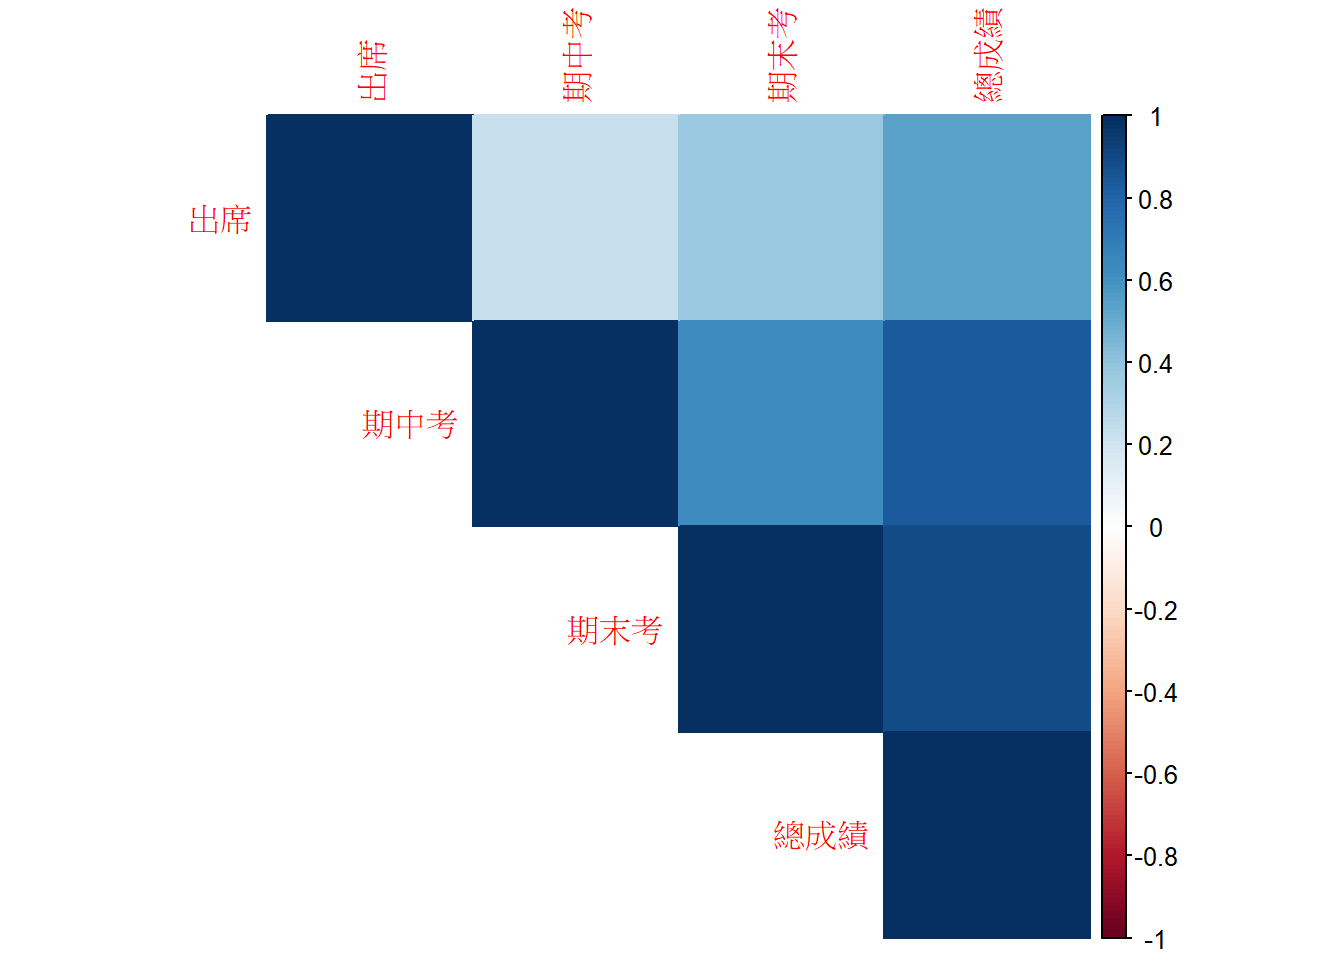
\includegraphics{quick-r-statistics_files/figure-latex/unnamed-chunk-49-1.pdf}

\hypertarget{hypotesting}{%
\chapter{假設檢定}\label{hypotesting}}

以R語言讀入資料並做假設檢定,包含常態檢定、獨立與相依t檢定。

\hypertarget{ux8b80ux5165ux6a94ux6848-2}{%
\section{讀入檔案}\label{ux8b80ux5165ux6a94ux6848-2}}

以xlsx套件的read.xlsx()函數或readxl套件的read\_xlsx()函數來讀入上個單元中所存出的\href{https://docs.google.com/spreadsheets/d/1qx6T0brgzuigBpS0p-Wq8hVSFFku9ebV/edit\#gid=390389518}{gData1.xlsx檔}。

\begin{Shaded}
\begin{Highlighting}[]
\FunctionTok{library}\NormalTok{(readxl)}
\NormalTok{gData1 }\OtherTok{\textless{}{-}} \FunctionTok{read\_xlsx}\NormalTok{(}\StringTok{"gData1.xlsx"}\NormalTok{)}
\FunctionTok{head}\NormalTok{(gData1)}
\end{Highlighting}
\end{Shaded}

\begin{verbatim}
## # A tibble: 6 x 8
##   學號      性別   組別  出席  影片 期中考 期末考 總成績
##   <chr>     <chr> <dbl> <dbl> <dbl>  <dbl>  <dbl>  <dbl>
## 1 102368014 M         9   8.5  82.6     32   28     56.0
## 2 102368018 M        10   9.5  82.9     66   59     78.8
## 3 102368024 F         9   8    82.6     69   68     81.2
## 4 102368027 F         9   8    82.6     68   83.5   86.0
## 5 102368030 F        11   0    66.5     39   30     45.2
## 6 100368033 M         4  12    73.3     58   79     82.1
\end{verbatim}

\hypertarget{ux5e38ux614bux6aa2ux5b9a}{%
\section{常態檢定}\label{ux5e38ux614bux6aa2ux5b9a}}

以qqnorm()和qqline()來看常態Q-Q圖。

\begin{Shaded}
\begin{Highlighting}[]
\FunctionTok{qqnorm}\NormalTok{(gData1}\SpecialCharTok{$}\NormalTok{總成績)}
\FunctionTok{qqline}\NormalTok{(gData1}\SpecialCharTok{$}\NormalTok{總成績)}
\end{Highlighting}
\end{Shaded}

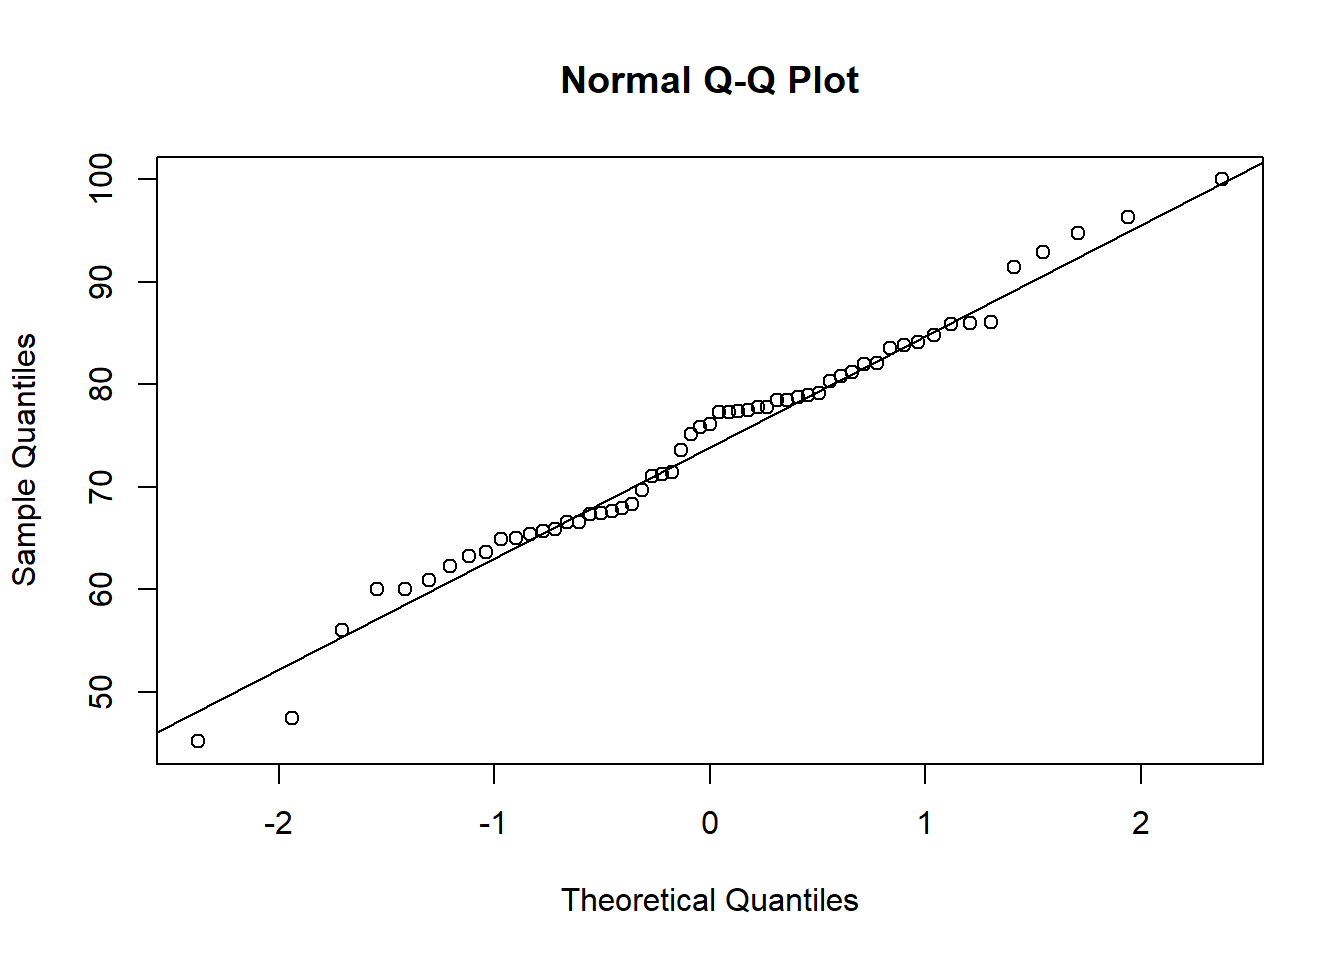
\includegraphics{quick-r-statistics_files/figure-latex/unnamed-chunk-52-1.pdf}

以shapiro.test()做常態檢定。

\begin{Shaded}
\begin{Highlighting}[]
\FunctionTok{shapiro.test}\NormalTok{(gData1}\SpecialCharTok{$}\NormalTok{總成績)}
\end{Highlighting}
\end{Shaded}

\begin{verbatim}
## 
##  Shapiro-Wilk normality test
## 
## data:  gData1$總成績
## W = 0.98346, p-value = 0.6243
\end{verbatim}

\hypertarget{ux7368ux7acbux6a23ux672ctux6aa2ux5b9a}{%
\section{獨立樣本t檢定}\label{ux7368ux7acbux6a23ux672ctux6aa2ux5b9a}}

先將性別轉為factor。

\begin{Shaded}
\begin{Highlighting}[]
\NormalTok{gData1}\SpecialCharTok{$}\NormalTok{性別 }\OtherTok{\textless{}{-}} \FunctionTok{factor}\NormalTok{(gData1}\SpecialCharTok{$}\NormalTok{性別)}
\end{Highlighting}
\end{Shaded}

以leveneTest()做變異數同質性檢定。

\begin{Shaded}
\begin{Highlighting}[]
\FunctionTok{library}\NormalTok{(car)}
\FunctionTok{leveneTest}\NormalTok{(gData1}\SpecialCharTok{$}\NormalTok{總成績 }\SpecialCharTok{\textasciitilde{}}\NormalTok{ gData1}\SpecialCharTok{$}\NormalTok{性別, }\AttributeTok{center=}\StringTok{"mean"}\NormalTok{)}
\end{Highlighting}
\end{Shaded}

\begin{verbatim}
## Levene's Test for Homogeneity of Variance (center = "mean")
##       Df F value Pr(>F)
## group  1  0.2112 0.6476
##       55
\end{verbatim}

以獨立樣本t檢定比較男女在總成績上是否有差異。

\begin{Shaded}
\begin{Highlighting}[]
\FunctionTok{t.test}\NormalTok{(gData1}\SpecialCharTok{$}\NormalTok{總成績 }\SpecialCharTok{\textasciitilde{}}\NormalTok{ gData1}\SpecialCharTok{$}\NormalTok{性別, }\AttributeTok{var.equal=}\ConstantTok{TRUE}\NormalTok{)}
\end{Highlighting}
\end{Shaded}

\begin{verbatim}
## 
##  Two Sample t-test
## 
## data:  gData1$總成績 by gData1$性別
## t = -0.62999, df = 55, p-value = 0.5313
## alternative hypothesis: true difference in means between group F and group M is not equal to 0
## 95 percent confidence interval:
##  -7.892010  4.116907
## sample estimates:
## mean in group F mean in group M 
##        73.43611        75.32366
\end{verbatim}

\hypertarget{ux76f8ux4f9dux6a23ux672ctux6aa2ux5b9a}{%
\section{相依樣本t檢定}\label{ux76f8ux4f9dux6a23ux672ctux6aa2ux5b9a}}

以t.test()做相依樣本t檢定,比較期中考和期末考是否有差異。

\begin{Shaded}
\begin{Highlighting}[]
\FunctionTok{t.test}\NormalTok{(gData1}\SpecialCharTok{$}\NormalTok{期中考, gData1}\SpecialCharTok{$}\NormalTok{期末考, }\AttributeTok{pair=}\ConstantTok{TRUE}\NormalTok{)}
\end{Highlighting}
\end{Shaded}

\begin{verbatim}
## 
##  Paired t-test
## 
## data:  gData1$期中考 and gData1$期末考
## t = -2.3616, df = 56, p-value = 0.0217
## alternative hypothesis: true mean difference is not equal to 0
## 95 percent confidence interval:
##  -8.3334024 -0.6841415
## sample estimates:
## mean difference 
##       -4.508772
\end{verbatim}

t.test()預設為雙尾檢定,若要做單尾檢定,可加入alternative的參數,可設定為''greater'' 或 ``less''。

\begin{Shaded}
\begin{Highlighting}[]
\FunctionTok{t.test}\NormalTok{(gData1}\SpecialCharTok{$}\NormalTok{期中考, gData1}\SpecialCharTok{$}\NormalTok{期末考, }\AttributeTok{alternative=}\StringTok{\textquotesingle{}less\textquotesingle{}}\NormalTok{,  }\AttributeTok{pair=}\ConstantTok{TRUE}\NormalTok{)}
\end{Highlighting}
\end{Shaded}

\begin{verbatim}
## 
##  Paired t-test
## 
## data:  gData1$期中考 and gData1$期末考
## t = -2.3616, df = 56, p-value = 0.01085
## alternative hypothesis: true mean difference is less than 0
## 95 percent confidence interval:
##       -Inf -1.315556
## sample estimates:
## mean difference 
##       -4.508772
\end{verbatim}

\hypertarget{within1way}{%
\chapter{相依樣本單因子變異數分析}\label{within1way}}

以R語言讀入資料並做相依樣本單因子變異數分析。

\hypertarget{ux8cc7ux6599ux6e96ux5099}{%
\section{資料準備}\label{ux8cc7ux6599ux6e96ux5099}}

\hypertarget{ux8b80ux5165ux6a94ux6848-3}{%
\subsection{讀入檔案}\label{ux8b80ux5165ux6a94ux6848-3}}

以xlsx套件的read.xlsx()函數或readxl套件的read\_xlsx()函數來讀入上個單元中所存出的\href{https://docs.google.com/spreadsheets/d/1qx6T0brgzuigBpS0p-Wq8hVSFFku9ebV/edit\#gid=390389518}{gData1.xlsx檔}。

\begin{Shaded}
\begin{Highlighting}[]
\FunctionTok{library}\NormalTok{(readxl)}
\NormalTok{gData1 }\OtherTok{\textless{}{-}} \FunctionTok{read\_xlsx}\NormalTok{(}\StringTok{"gData1.xlsx"}\NormalTok{)}
\FunctionTok{head}\NormalTok{(gData1)}
\end{Highlighting}
\end{Shaded}

\begin{verbatim}
## # A tibble: 6 x 8
##   學號      性別   組別  出席  影片 期中考 期末考 總成績
##   <chr>     <chr> <dbl> <dbl> <dbl>  <dbl>  <dbl>  <dbl>
## 1 102368014 M         9   8.5  82.6     32   28     56.0
## 2 102368018 M        10   9.5  82.9     66   59     78.8
## 3 102368024 F         9   8    82.6     69   68     81.2
## 4 102368027 F         9   8    82.6     68   83.5   86.0
## 5 102368030 F        11   0    66.5     39   30     45.2
## 6 100368033 M         4  12    73.3     58   79     82.1
\end{verbatim}

\hypertarget{ux6e96ux5099ux53efux4f9bux8b8aux7570ux6578ux5206ux6790ux7684ux8cc7ux6599}{%
\subsection{準備可供變異數分析的資料}\label{ux6e96ux5099ux53efux4f9bux8b8aux7570ux6578ux5206ux6790ux7684ux8cc7ux6599}}

新增一假設的期初考成績,以做為變異數分析之用。

\begin{Shaded}
\begin{Highlighting}[]
\FunctionTok{library}\NormalTok{(tibble)}
\NormalTok{gData1 }\OtherTok{\textless{}{-}} \FunctionTok{add\_column}\NormalTok{(gData1, 期初考}\OtherTok{=}\NormalTok{gData1}\SpecialCharTok{$}\NormalTok{出席}\SpecialCharTok{*}\DecValTok{8}\NormalTok{, }\AttributeTok{.after =} \DecValTok{5}\NormalTok{)}
\FunctionTok{head}\NormalTok{(gData1)}
\end{Highlighting}
\end{Shaded}

\begin{verbatim}
## # A tibble: 6 x 9
##   學號      性別   組別  出席  影片 期初考 期中考 期末考 總成績
##   <chr>     <chr> <dbl> <dbl> <dbl>  <dbl>  <dbl>  <dbl>  <dbl>
## 1 102368014 M         9   8.5  82.6     68     32   28     56.0
## 2 102368018 M        10   9.5  82.9     76     66   59     78.8
## 3 102368024 F         9   8    82.6     64     69   68     81.2
## 4 102368027 F         9   8    82.6     64     68   83.5   86.0
## 5 102368030 F        11   0    66.5      0     39   30     45.2
## 6 100368033 M         4  12    73.3     96     58   79     82.1
\end{verbatim}

選擇期初考、期中考和期末考進來分析,並加入編號(亦可使用學號,這邊方便起見加入編號來做)。

\begin{Shaded}
\begin{Highlighting}[]
\NormalTok{gData3 }\OtherTok{\textless{}{-}} \FunctionTok{subset}\NormalTok{(gData1, }\AttributeTok{select =} \FunctionTok{c}\NormalTok{(期初考, 期中考, 期末考))}
\NormalTok{gData3 }\OtherTok{\textless{}{-}} \FunctionTok{add\_column}\NormalTok{(gData3, }\AttributeTok{id =} \FunctionTok{c}\NormalTok{(}\DecValTok{1}\SpecialCharTok{:}\FunctionTok{nrow}\NormalTok{(gData3)), }\AttributeTok{.after =} \DecValTok{0}\NormalTok{)}
\FunctionTok{head}\NormalTok{(gData3)}
\end{Highlighting}
\end{Shaded}

\begin{verbatim}
## # A tibble: 6 x 4
##      id 期初考 期中考 期末考
##   <int>  <dbl>  <dbl>  <dbl>
## 1     1     68     32   28  
## 2     2     76     66   59  
## 3     3     64     69   68  
## 4     4     64     68   83.5
## 5     5      0     39   30  
## 6     6     96     58   79
\end{verbatim}

用reshape2套件的melt()函數,將期初、期中、期末考合併為一行。

\begin{Shaded}
\begin{Highlighting}[]
\FunctionTok{library}\NormalTok{(reshape2)}
\NormalTok{gData3m }\OtherTok{\textless{}{-}} \FunctionTok{melt}\NormalTok{(gData3, }\AttributeTok{id =} \FunctionTok{c}\NormalTok{(}\StringTok{"id"}\NormalTok{), }\AttributeTok{measured =} \FunctionTok{c}\NormalTok{(}\StringTok{"期初考"}\NormalTok{, }\StringTok{"期中考"}\NormalTok{, }\StringTok{"期末考"}\NormalTok{))}
\FunctionTok{head}\NormalTok{(gData3m)}
\end{Highlighting}
\end{Shaded}

\begin{verbatim}
##   id variable value
## 1  1   期初考    68
## 2  2   期初考    76
## 3  3   期初考    64
## 4  4   期初考    64
## 5  5   期初考     0
## 6  6   期初考    96
\end{verbatim}

更改column的名稱。

\begin{Shaded}
\begin{Highlighting}[]
\FunctionTok{names}\NormalTok{(gData3m) }\OtherTok{\textless{}{-}} \FunctionTok{c}\NormalTok{(}\StringTok{\textquotesingle{}編號\textquotesingle{}}\NormalTok{, }\StringTok{\textquotesingle{}考試\textquotesingle{}}\NormalTok{, }\StringTok{\textquotesingle{}成績\textquotesingle{}}\NormalTok{)}
\FunctionTok{head}\NormalTok{(gData3m)}
\end{Highlighting}
\end{Shaded}

\begin{verbatim}
##   編號   考試 成績
## 1    1 期初考   68
## 2    2 期初考   76
## 3    3 期初考   64
## 4    4 期初考   64
## 5    5 期初考    0
## 6    6 期初考   96
\end{verbatim}

以上資料格式即為變異數分析所需的格式。

在執行相依樣本單因子變異數分析時,要注意的是,資料必須如此例這般,不同組的資料以「接續」的方式排列。若拿到的資料是一般相依樣本的資料輸入方式(即不同組在不同的columns),需先進行資料的處理,將wide data轉為long data,再做相依樣本單因子變異數分析。

\hypertarget{ux63cfux8ff0ux7d71ux8a08-1}{%
\section{描述統計}\label{ux63cfux8ff0ux7d71ux8a08-1}}

檢視三次考試的平均數和標準差。

\begin{Shaded}
\begin{Highlighting}[]
\FunctionTok{library}\NormalTok{(vtable)}
\FunctionTok{st}\NormalTok{(gData3m, }\AttributeTok{group=}\StringTok{\textquotesingle{}考試\textquotesingle{}}\NormalTok{)}
\end{Highlighting}
\end{Shaded}

\begin{table}

\caption{\label{tab:unnamed-chunk-65}Summary Statistics}
\centering
\begin{tabular}[t]{llllllllll}
\toprule
\multicolumn{1}{c}{考試} & \multicolumn{3}{c}{期初考} & \multicolumn{3}{c}{期中考} & \multicolumn{3}{c}{期末考} \\
\cmidrule(l{3pt}r{3pt}){1-1} \cmidrule(l{3pt}r{3pt}){2-4} \cmidrule(l{3pt}r{3pt}){5-7} \cmidrule(l{3pt}r{3pt}){8-10}
Variable & N & Mean & SD & N & Mean & SD & N & Mean & SD\\
\midrule
編號 & 57 & 29 & 16.598 & 57 & 29 & 16.598 & 57 & 29 & 16.598\\
成績 & 57 & 82.807 & 18.485 & 57 & 54.947 & 13.313 & 57 & 59.456 & 18.216\\
\bottomrule
\end{tabular}
\end{table}

以boxplot來看作圖。

\begin{Shaded}
\begin{Highlighting}[]
\FunctionTok{boxplot}\NormalTok{(成績}\SpecialCharTok{\textasciitilde{}}\NormalTok{考試, }\AttributeTok{data=}\NormalTok{gData3m)}
\end{Highlighting}
\end{Shaded}

\begin{verbatim}
## Warning in axis(side = base::quote(1), at = base::quote(1:3), labels =
## base::quote(c("期初考", : conversion failure on '期初考' in 'mbcsToSbcs': dot
## substituted for <e6>
\end{verbatim}

\begin{verbatim}
## Warning in axis(side = base::quote(1), at = base::quote(1:3), labels =
## base::quote(c("期初考", : conversion failure on '期初考' in 'mbcsToSbcs': dot
## substituted for <9c>
\end{verbatim}

\begin{verbatim}
## Warning in axis(side = base::quote(1), at = base::quote(1:3), labels =
## base::quote(c("期初考", : conversion failure on '期初考' in 'mbcsToSbcs': dot
## substituted for <9f>
\end{verbatim}

\begin{verbatim}
## Warning in axis(side = base::quote(1), at = base::quote(1:3), labels =
## base::quote(c("期初考", : conversion failure on '期初考' in 'mbcsToSbcs': dot
## substituted for <e5>
\end{verbatim}

\begin{verbatim}
## Warning in axis(side = base::quote(1), at = base::quote(1:3), labels =
## base::quote(c("期初考", : conversion failure on '期初考' in 'mbcsToSbcs': dot
## substituted for <88>
\end{verbatim}

\begin{verbatim}
## Warning in axis(side = base::quote(1), at = base::quote(1:3), labels =
## base::quote(c("期初考", : conversion failure on '期初考' in 'mbcsToSbcs': dot
## substituted for <9d>
\end{verbatim}

\begin{verbatim}
## Warning in axis(side = base::quote(1), at = base::quote(1:3), labels =
## base::quote(c("期初考", : conversion failure on '期初考' in 'mbcsToSbcs': dot
## substituted for <e8>
\end{verbatim}

\begin{verbatim}
## Warning in axis(side = base::quote(1), at = base::quote(1:3), labels =
## base::quote(c("期初考", : conversion failure on '期初考' in 'mbcsToSbcs': dot
## substituted for <80>
\end{verbatim}

\begin{verbatim}
## Warning in axis(side = base::quote(1), at = base::quote(1:3), labels =
## base::quote(c("期初考", : conversion failure on '期初考' in 'mbcsToSbcs': dot
## substituted for <83>
\end{verbatim}

\begin{verbatim}
## Warning in axis(side = base::quote(1), at = base::quote(1:3), labels =
## base::quote(c("期初考", : conversion failure on '期初考' in 'mbcsToSbcs': dot
## substituted for <e6>
\end{verbatim}

\begin{verbatim}
## Warning in axis(side = base::quote(1), at = base::quote(1:3), labels =
## base::quote(c("期初考", : conversion failure on '期初考' in 'mbcsToSbcs': dot
## substituted for <9c>
\end{verbatim}

\begin{verbatim}
## Warning in axis(side = base::quote(1), at = base::quote(1:3), labels =
## base::quote(c("期初考", : conversion failure on '期初考' in 'mbcsToSbcs': dot
## substituted for <9f>
\end{verbatim}

\begin{verbatim}
## Warning in axis(side = base::quote(1), at = base::quote(1:3), labels =
## base::quote(c("期初考", : conversion failure on '期初考' in 'mbcsToSbcs': dot
## substituted for <e5>
\end{verbatim}

\begin{verbatim}
## Warning in axis(side = base::quote(1), at = base::quote(1:3), labels =
## base::quote(c("期初考", : conversion failure on '期初考' in 'mbcsToSbcs': dot
## substituted for <88>
\end{verbatim}

\begin{verbatim}
## Warning in axis(side = base::quote(1), at = base::quote(1:3), labels =
## base::quote(c("期初考", : conversion failure on '期初考' in 'mbcsToSbcs': dot
## substituted for <9d>
\end{verbatim}

\begin{verbatim}
## Warning in axis(side = base::quote(1), at = base::quote(1:3), labels =
## base::quote(c("期初考", : conversion failure on '期初考' in 'mbcsToSbcs': dot
## substituted for <e8>
\end{verbatim}

\begin{verbatim}
## Warning in axis(side = base::quote(1), at = base::quote(1:3), labels =
## base::quote(c("期初考", : conversion failure on '期初考' in 'mbcsToSbcs': dot
## substituted for <80>
\end{verbatim}

\begin{verbatim}
## Warning in axis(side = base::quote(1), at = base::quote(1:3), labels =
## base::quote(c("期初考", : conversion failure on '期初考' in 'mbcsToSbcs': dot
## substituted for <83>
\end{verbatim}

\begin{verbatim}
## Warning in axis(side = base::quote(1), at = base::quote(1:3), labels =
## base::quote(c("期初考", : conversion failure on '期中考' in 'mbcsToSbcs': dot
## substituted for <e6>
\end{verbatim}

\begin{verbatim}
## Warning in axis(side = base::quote(1), at = base::quote(1:3), labels =
## base::quote(c("期初考", : conversion failure on '期中考' in 'mbcsToSbcs': dot
## substituted for <9c>
\end{verbatim}

\begin{verbatim}
## Warning in axis(side = base::quote(1), at = base::quote(1:3), labels =
## base::quote(c("期初考", : conversion failure on '期中考' in 'mbcsToSbcs': dot
## substituted for <9f>
\end{verbatim}

\begin{verbatim}
## Warning in axis(side = base::quote(1), at = base::quote(1:3), labels =
## base::quote(c("期初考", : conversion failure on '期中考' in 'mbcsToSbcs': dot
## substituted for <e4>
\end{verbatim}

\begin{verbatim}
## Warning in axis(side = base::quote(1), at = base::quote(1:3), labels =
## base::quote(c("期初考", : conversion failure on '期中考' in 'mbcsToSbcs': dot
## substituted for <b8>
\end{verbatim}

\begin{verbatim}
## Warning in axis(side = base::quote(1), at = base::quote(1:3), labels =
## base::quote(c("期初考", : conversion failure on '期中考' in 'mbcsToSbcs': dot
## substituted for <ad>
\end{verbatim}

\begin{verbatim}
## Warning in axis(side = base::quote(1), at = base::quote(1:3), labels =
## base::quote(c("期初考", : conversion failure on '期中考' in 'mbcsToSbcs': dot
## substituted for <e8>
\end{verbatim}

\begin{verbatim}
## Warning in axis(side = base::quote(1), at = base::quote(1:3), labels =
## base::quote(c("期初考", : conversion failure on '期中考' in 'mbcsToSbcs': dot
## substituted for <80>
\end{verbatim}

\begin{verbatim}
## Warning in axis(side = base::quote(1), at = base::quote(1:3), labels =
## base::quote(c("期初考", : conversion failure on '期中考' in 'mbcsToSbcs': dot
## substituted for <83>
\end{verbatim}

\begin{verbatim}
## Warning in axis(side = base::quote(1), at = base::quote(1:3), labels =
## base::quote(c("期初考", : conversion failure on '期中考' in 'mbcsToSbcs': dot
## substituted for <e6>
\end{verbatim}

\begin{verbatim}
## Warning in axis(side = base::quote(1), at = base::quote(1:3), labels =
## base::quote(c("期初考", : conversion failure on '期中考' in 'mbcsToSbcs': dot
## substituted for <9c>
\end{verbatim}

\begin{verbatim}
## Warning in axis(side = base::quote(1), at = base::quote(1:3), labels =
## base::quote(c("期初考", : conversion failure on '期中考' in 'mbcsToSbcs': dot
## substituted for <9f>
\end{verbatim}

\begin{verbatim}
## Warning in axis(side = base::quote(1), at = base::quote(1:3), labels =
## base::quote(c("期初考", : conversion failure on '期中考' in 'mbcsToSbcs': dot
## substituted for <e4>
\end{verbatim}

\begin{verbatim}
## Warning in axis(side = base::quote(1), at = base::quote(1:3), labels =
## base::quote(c("期初考", : conversion failure on '期中考' in 'mbcsToSbcs': dot
## substituted for <b8>
\end{verbatim}

\begin{verbatim}
## Warning in axis(side = base::quote(1), at = base::quote(1:3), labels =
## base::quote(c("期初考", : conversion failure on '期中考' in 'mbcsToSbcs': dot
## substituted for <ad>
\end{verbatim}

\begin{verbatim}
## Warning in axis(side = base::quote(1), at = base::quote(1:3), labels =
## base::quote(c("期初考", : conversion failure on '期中考' in 'mbcsToSbcs': dot
## substituted for <e8>
\end{verbatim}

\begin{verbatim}
## Warning in axis(side = base::quote(1), at = base::quote(1:3), labels =
## base::quote(c("期初考", : conversion failure on '期中考' in 'mbcsToSbcs': dot
## substituted for <80>
\end{verbatim}

\begin{verbatim}
## Warning in axis(side = base::quote(1), at = base::quote(1:3), labels =
## base::quote(c("期初考", : conversion failure on '期中考' in 'mbcsToSbcs': dot
## substituted for <83>
\end{verbatim}

\begin{verbatim}
## Warning in axis(side = base::quote(1), at = base::quote(1:3), labels =
## base::quote(c("期初考", : conversion failure on '期末考' in 'mbcsToSbcs': dot
## substituted for <e6>
\end{verbatim}

\begin{verbatim}
## Warning in axis(side = base::quote(1), at = base::quote(1:3), labels =
## base::quote(c("期初考", : conversion failure on '期末考' in 'mbcsToSbcs': dot
## substituted for <9c>
\end{verbatim}

\begin{verbatim}
## Warning in axis(side = base::quote(1), at = base::quote(1:3), labels =
## base::quote(c("期初考", : conversion failure on '期末考' in 'mbcsToSbcs': dot
## substituted for <9f>
\end{verbatim}

\begin{verbatim}
## Warning in axis(side = base::quote(1), at = base::quote(1:3), labels =
## base::quote(c("期初考", : conversion failure on '期末考' in 'mbcsToSbcs': dot
## substituted for <e6>
\end{verbatim}

\begin{verbatim}
## Warning in axis(side = base::quote(1), at = base::quote(1:3), labels =
## base::quote(c("期初考", : conversion failure on '期末考' in 'mbcsToSbcs': dot
## substituted for <9c>
\end{verbatim}

\begin{verbatim}
## Warning in axis(side = base::quote(1), at = base::quote(1:3), labels =
## base::quote(c("期初考", : conversion failure on '期末考' in 'mbcsToSbcs': dot
## substituted for <ab>
\end{verbatim}

\begin{verbatim}
## Warning in axis(side = base::quote(1), at = base::quote(1:3), labels =
## base::quote(c("期初考", : conversion failure on '期末考' in 'mbcsToSbcs': dot
## substituted for <e8>
\end{verbatim}

\begin{verbatim}
## Warning in axis(side = base::quote(1), at = base::quote(1:3), labels =
## base::quote(c("期初考", : conversion failure on '期末考' in 'mbcsToSbcs': dot
## substituted for <80>
\end{verbatim}

\begin{verbatim}
## Warning in axis(side = base::quote(1), at = base::quote(1:3), labels =
## base::quote(c("期初考", : conversion failure on '期末考' in 'mbcsToSbcs': dot
## substituted for <83>
\end{verbatim}

\begin{verbatim}
## Warning in axis(side = base::quote(1), at = base::quote(1:3), labels =
## base::quote(c("期初考", : conversion failure on '期末考' in 'mbcsToSbcs': dot
## substituted for <e6>
\end{verbatim}

\begin{verbatim}
## Warning in axis(side = base::quote(1), at = base::quote(1:3), labels =
## base::quote(c("期初考", : conversion failure on '期末考' in 'mbcsToSbcs': dot
## substituted for <9c>
\end{verbatim}

\begin{verbatim}
## Warning in axis(side = base::quote(1), at = base::quote(1:3), labels =
## base::quote(c("期初考", : conversion failure on '期末考' in 'mbcsToSbcs': dot
## substituted for <9f>
\end{verbatim}

\begin{verbatim}
## Warning in axis(side = base::quote(1), at = base::quote(1:3), labels =
## base::quote(c("期初考", : conversion failure on '期末考' in 'mbcsToSbcs': dot
## substituted for <e6>
\end{verbatim}

\begin{verbatim}
## Warning in axis(side = base::quote(1), at = base::quote(1:3), labels =
## base::quote(c("期初考", : conversion failure on '期末考' in 'mbcsToSbcs': dot
## substituted for <9c>
\end{verbatim}

\begin{verbatim}
## Warning in axis(side = base::quote(1), at = base::quote(1:3), labels =
## base::quote(c("期初考", : conversion failure on '期末考' in 'mbcsToSbcs': dot
## substituted for <ab>
\end{verbatim}

\begin{verbatim}
## Warning in axis(side = base::quote(1), at = base::quote(1:3), labels =
## base::quote(c("期初考", : conversion failure on '期末考' in 'mbcsToSbcs': dot
## substituted for <e8>
\end{verbatim}

\begin{verbatim}
## Warning in axis(side = base::quote(1), at = base::quote(1:3), labels =
## base::quote(c("期初考", : conversion failure on '期末考' in 'mbcsToSbcs': dot
## substituted for <80>
\end{verbatim}

\begin{verbatim}
## Warning in axis(side = base::quote(1), at = base::quote(1:3), labels =
## base::quote(c("期初考", : conversion failure on '期末考' in 'mbcsToSbcs': dot
## substituted for <83>
\end{verbatim}

\begin{verbatim}
## Warning in (function (main = NULL, sub = NULL, xlab = NULL, ylab = NULL, :
## conversion failure on '考試' in 'mbcsToSbcs': dot substituted for <e8>
\end{verbatim}

\begin{verbatim}
## Warning in (function (main = NULL, sub = NULL, xlab = NULL, ylab = NULL, :
## conversion failure on '考試' in 'mbcsToSbcs': dot substituted for <80>
\end{verbatim}

\begin{verbatim}
## Warning in (function (main = NULL, sub = NULL, xlab = NULL, ylab = NULL, :
## conversion failure on '考試' in 'mbcsToSbcs': dot substituted for <83>
\end{verbatim}

\begin{verbatim}
## Warning in (function (main = NULL, sub = NULL, xlab = NULL, ylab = NULL, :
## conversion failure on '考試' in 'mbcsToSbcs': dot substituted for <e8>
\end{verbatim}

\begin{verbatim}
## Warning in (function (main = NULL, sub = NULL, xlab = NULL, ylab = NULL, :
## conversion failure on '考試' in 'mbcsToSbcs': dot substituted for <a9>
\end{verbatim}

\begin{verbatim}
## Warning in (function (main = NULL, sub = NULL, xlab = NULL, ylab = NULL, :
## conversion failure on '考試' in 'mbcsToSbcs': dot substituted for <a6>
\end{verbatim}

\begin{verbatim}
## Warning in (function (main = NULL, sub = NULL, xlab = NULL, ylab = NULL, :
## conversion failure on '成績' in 'mbcsToSbcs': dot substituted for <e6>
\end{verbatim}

\begin{verbatim}
## Warning in (function (main = NULL, sub = NULL, xlab = NULL, ylab = NULL, :
## conversion failure on '成績' in 'mbcsToSbcs': dot substituted for <88>
\end{verbatim}

\begin{verbatim}
## Warning in (function (main = NULL, sub = NULL, xlab = NULL, ylab = NULL, :
## conversion failure on '成績' in 'mbcsToSbcs': dot substituted for <90>
\end{verbatim}

\begin{verbatim}
## Warning in (function (main = NULL, sub = NULL, xlab = NULL, ylab = NULL, :
## conversion failure on '成績' in 'mbcsToSbcs': dot substituted for <e7>
\end{verbatim}

\begin{verbatim}
## Warning in (function (main = NULL, sub = NULL, xlab = NULL, ylab = NULL, :
## conversion failure on '成績' in 'mbcsToSbcs': dot substituted for <b8>
\end{verbatim}

\begin{verbatim}
## Warning in (function (main = NULL, sub = NULL, xlab = NULL, ylab = NULL, :
## conversion failure on '成績' in 'mbcsToSbcs': dot substituted for <be>
\end{verbatim}

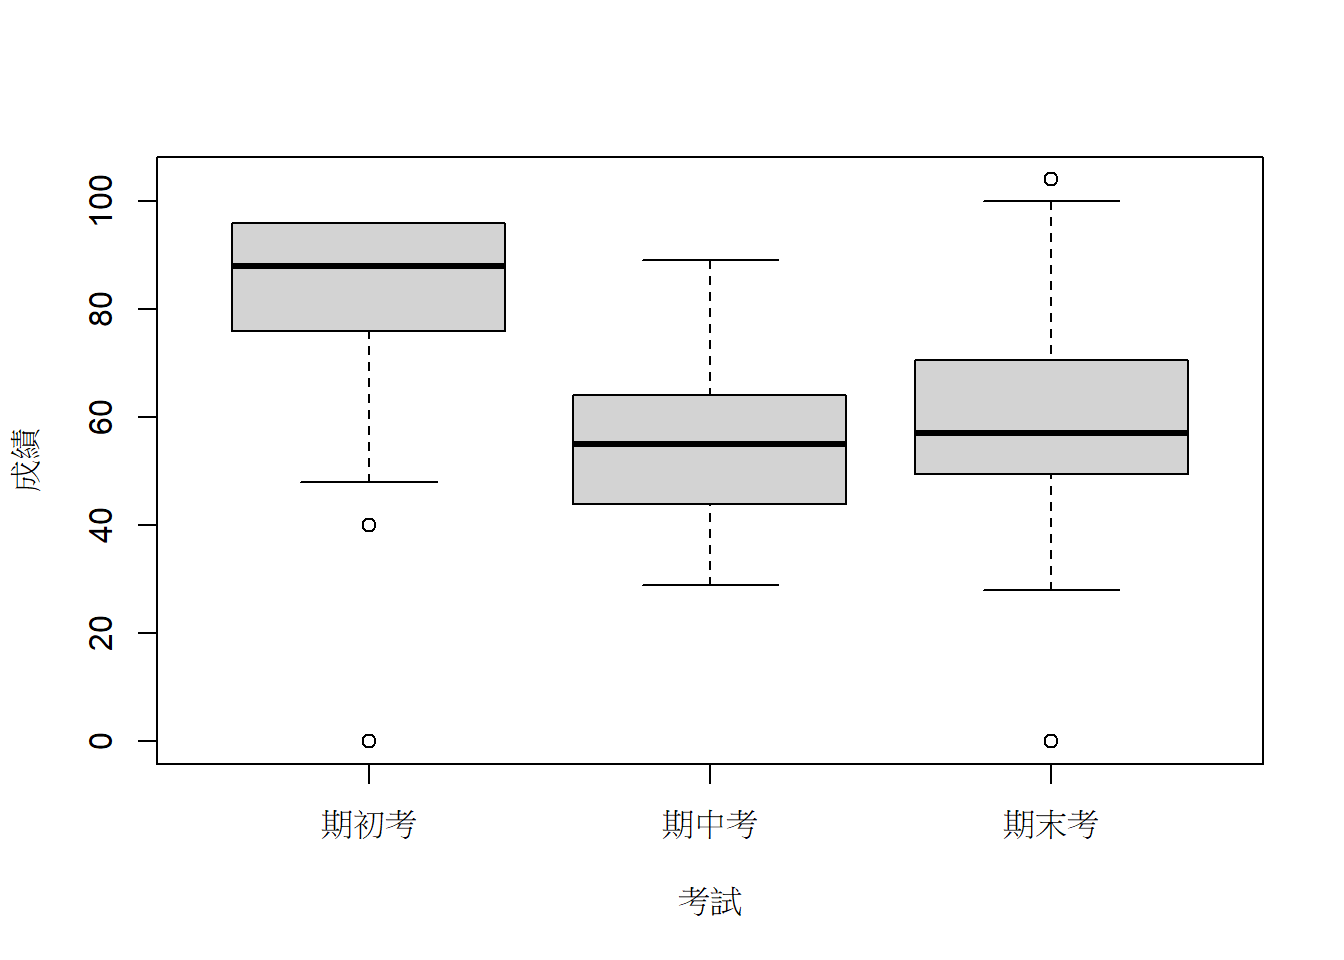
\includegraphics{quick-r-statistics_files/figure-latex/unnamed-chunk-67-1.pdf}

以ggpubr套件的ggline函數來作圖,畫平均數和標準差。

\begin{Shaded}
\begin{Highlighting}[]
\FunctionTok{library}\NormalTok{(ggpubr)}
\FunctionTok{ggline}\NormalTok{(gData3m,}\AttributeTok{x=}\StringTok{"考試"}\NormalTok{,}\AttributeTok{y=}\StringTok{"成績"}\NormalTok{,}\AttributeTok{add=}\FunctionTok{c}\NormalTok{(}\StringTok{"mean\_sd"}\NormalTok{))}
\end{Highlighting}
\end{Shaded}

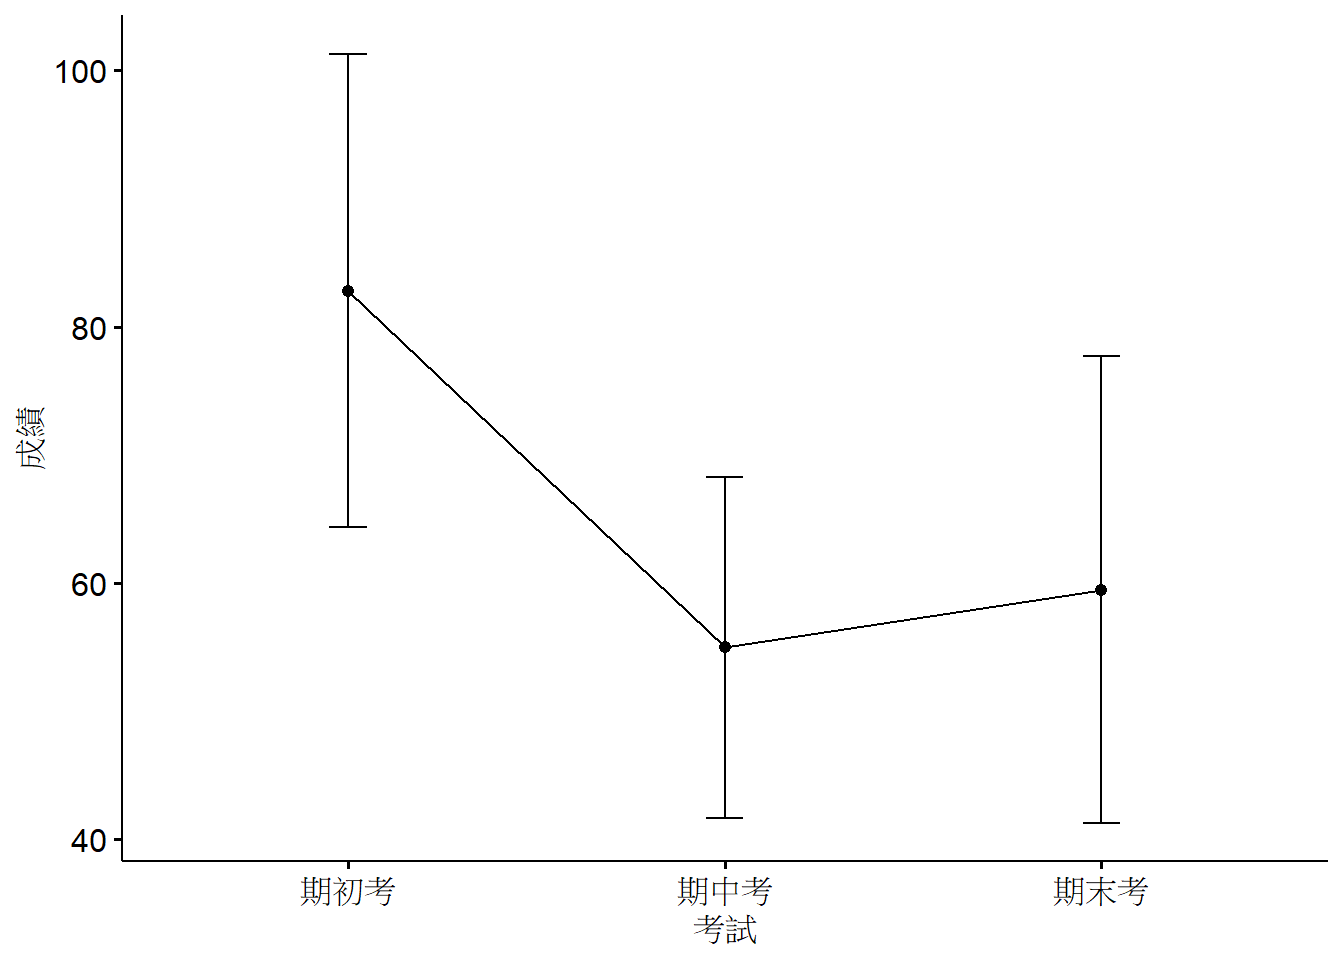
\includegraphics{quick-r-statistics_files/figure-latex/unnamed-chunk-68-1.pdf}

\hypertarget{ux8b8aux7570ux6578ux5206ux6790}{%
\section{變異數分析}\label{ux8b8aux7570ux6578ux5206ux6790}}

先將編號的格式改為factor。

\begin{Shaded}
\begin{Highlighting}[]
\NormalTok{gData3m}\SpecialCharTok{$}\NormalTok{編號 }\OtherTok{\textless{}{-}} \FunctionTok{factor}\NormalTok{(gData3m}\SpecialCharTok{$}\NormalTok{編號)}
\FunctionTok{head}\NormalTok{(gData3m)}
\end{Highlighting}
\end{Shaded}

\begin{verbatim}
##   編號   考試 成績
## 1    1 期初考   68
## 2    2 期初考   76
## 3    3 期初考   64
## 4    4 期初考   64
## 5    5 期初考    0
## 6    6 期初考   96
\end{verbatim}

\hypertarget{ux7403ux578bux6aa2ux5b9aux8207ux8b8aux7570ux6578ux5206ux6790}{%
\subsection{球型檢定與變異數分析}\label{ux7403ux578bux6aa2ux5b9aux8207ux8b8aux7570ux6578ux5206ux6790}}

用rstatix package中的anova\_test()來做變異數分析,將結果儲存為res。並以res來看檢驗的結果。

因本資料違反球型檢定,需要看sphericity correction的表。Sphericity Corrections以Greenhouse-Geisser (GG)和Huynh-Feldt (HF) epsilon values來做校正。校正後的值 p{[}GG{]} 和 p{[}HF{]} 皆小於.001,表示不同考試成績有顯著差異。

\begin{Shaded}
\begin{Highlighting}[]
\FunctionTok{library}\NormalTok{(rstatix)}
\NormalTok{res }\OtherTok{\textless{}{-}} \FunctionTok{anova\_test}\NormalTok{(}\AttributeTok{data =}\NormalTok{ gData3m, }\AttributeTok{dv =}\NormalTok{ 成績, }\AttributeTok{wid =}\NormalTok{ 編號, }\AttributeTok{within =}\NormalTok{ 考試)}
\NormalTok{res}
\end{Highlighting}
\end{Shaded}

\begin{verbatim}
## ANOVA Table (type III tests)
## 
## $ANOVA
##   Effect DFn DFd      F        p p<.05   ges
## 1   考試   2 112 73.704 3.74e-21     * 0.349
## 
## $`Mauchly's Test for Sphericity`
##   Effect    W     p p<.05
## 1   考試 0.84 0.008     *
## 
## $`Sphericity Corrections`
##   Effect   GGe      DF[GG]   p[GG] p[GG]<.05   HFe      DF[HF]   p[HF]
## 1   考試 0.862 1.72, 96.57 1.4e-18         * 0.887 1.77, 99.36 4.8e-19
##   p[HF]<.05
## 1         *
\end{verbatim}

最後,用get\_anova\_table()來看校正後的結果。校正的結果顯示,F(1.72, 96.57) = 73.704, p \textless{} .001。三次考試的成績顯著不同。

\begin{Shaded}
\begin{Highlighting}[]
\FunctionTok{get\_anova\_table}\NormalTok{(res)}
\end{Highlighting}
\end{Shaded}

\begin{verbatim}
## ANOVA Table (type III tests)
## 
##   Effect  DFn   DFd      F       p p<.05   ges
## 1   考試 1.72 96.57 73.704 1.4e-18     * 0.349
\end{verbatim}

\hypertarget{ux591aux91cdux6bd4ux8f03}{%
\subsection{多重比較}\label{ux591aux91cdux6bd4ux8f03}}

可用pairwise\_t\_test()來做兩兩比較,看差異來自於哪裡。結果顯示期中和期末考沒有差異,其餘兩兩比較都有差異。

\begin{Shaded}
\begin{Highlighting}[]
\FunctionTok{pairwise\_t\_test}\NormalTok{(gData3m, 成績 }\SpecialCharTok{\textasciitilde{}}\NormalTok{ 考試, }\AttributeTok{paired =} \ConstantTok{TRUE}\NormalTok{, }\AttributeTok{p.adjust.method =} \StringTok{"bonferroni"}\NormalTok{)}
\end{Highlighting}
\end{Shaded}

\begin{verbatim}
## # A tibble: 3 x 10
##   .y.   group1 group2    n1    n2 statistic    df        p    p.adj p.adj.signif
## * <chr> <chr>  <chr>  <int> <int>     <dbl> <dbl>    <dbl>    <dbl> <chr>       
## 1 成績  期初考 期中考    57    57     10.4     56 1.11e-14 3.33e-14 ****        
## 2 成績  期初考 期末考    57    57      8.60    56 8.06e-12 2.42e-11 ****        
## 3 成績  期中考 期末考    57    57     -2.36    56 2.2 e- 2 6.5 e- 2 ns
\end{verbatim}

\hypertarget{ux82e5ux672aux9055ux53cdux7403ux578bux6aa2ux5b9a}{%
\subsection{若未違反球型檢定}\label{ux82e5ux672aux9055ux53cdux7403ux578bux6aa2ux5b9a}}

若是球型檢定沒有違反,也可以用aov()來做變異數分析。在aov()中,以y\textasciitilde factor(x)+Error(factor(Subj)/factor(x))來執行變異數分析。

\begin{Shaded}
\begin{Highlighting}[]
\NormalTok{ANOVAData }\OtherTok{\textless{}{-}} \FunctionTok{aov}\NormalTok{(成績}\SpecialCharTok{\textasciitilde{}}\FunctionTok{factor}\NormalTok{(考試)}\SpecialCharTok{+}\FunctionTok{Error}\NormalTok{(}\FunctionTok{factor}\NormalTok{(編號)}\SpecialCharTok{/}\FunctionTok{factor}\NormalTok{(考試)), }\AttributeTok{data=}\NormalTok{gData3m)}
\end{Highlighting}
\end{Shaded}

以model.tables()來看各組的邊緣平均數(marginal mean)和總平均數(ground mean)。總平均數為65.74,期初、期中和期末考的平均數分別為82.81、54.95與59.46。

\begin{Shaded}
\begin{Highlighting}[]
\FunctionTok{model.tables}\NormalTok{(ANOVAData,}\AttributeTok{type=}\StringTok{"means"}\NormalTok{)}
\end{Highlighting}
\end{Shaded}

\begin{verbatim}
## Tables of means
## Grand mean
##          
## 65.73684 
## 
##  factor(考試) 
## factor(考試)
## 期初考 期中考 期末考 
##  82.81  54.95  59.46
\end{verbatim}

以summary()來看ANOVA table。可得到F(2,112)=73.7,p\textless.001,表示三次考試的成績有顯著差異。

\begin{Shaded}
\begin{Highlighting}[]
\FunctionTok{summary}\NormalTok{(ANOVAData,}\AttributeTok{type=}\StringTok{"means"}\NormalTok{)}
\end{Highlighting}
\end{Shaded}

\begin{verbatim}
## 
## Error: factor(編號)
##           Df Sum Sq Mean Sq F value Pr(>F)
## Residuals 56  28272   504.9               
## 
## Error: factor(編號):factor(考試)
##               Df Sum Sq Mean Sq F value Pr(>F)    
## factor(考試)   2  25493   12747    73.7 <2e-16 ***
## Residuals    112  19370     173                   
## ---
## Signif. codes:  0 '***' 0.001 '**' 0.01 '*' 0.05 '.' 0.1 ' ' 1
\end{verbatim}

\hypertarget{between1way}{%
\chapter{獨立樣本單因子變異數分析}\label{between1way}}

以R語言讀入資料並做獨立樣本單因子變異數分析。

\hypertarget{ux8cc7ux6599ux6e96ux5099-1}{%
\section{資料準備}\label{ux8cc7ux6599ux6e96ux5099-1}}

\hypertarget{ux8b80ux5165ux6a94ux6848-4}{%
\subsection{讀入檔案}\label{ux8b80ux5165ux6a94ux6848-4}}

接續前一單元,以gData3m變數來做分析,或以xlsx套件的read.xlsx()函數或readxl套件的read\_xlsx()函數來讀入\href{https://docs.google.com/spreadsheets/d/1kJlbaSGZ5ioTz6DZ56yHLYxjDWO9t92t/edit\#gid=1205378113}{gData3m.xlsx檔}。

\begin{Shaded}
\begin{Highlighting}[]
\FunctionTok{library}\NormalTok{(readxl)}
\NormalTok{gData3m }\OtherTok{\textless{}{-}} \FunctionTok{read\_xlsx}\NormalTok{(}\StringTok{"gData3m.xlsx"}\NormalTok{)}
\FunctionTok{head}\NormalTok{(gData3m)}
\end{Highlighting}
\end{Shaded}

\begin{verbatim}
## # A tibble: 6 x 3
##   編號  考試    成績
##   <chr> <chr>  <dbl>
## 1 1     期初考    68
## 2 2     期初考    76
## 3 3     期初考    64
## 4 4     期初考    64
## 5 5     期初考     0
## 6 6     期初考    96
\end{verbatim}

\hypertarget{ux6e96ux5099ux53efux4f9bux8b8aux7570ux6578ux5206ux6790ux7684ux8cc7ux6599-1}{%
\subsection{準備可供變異數分析的資料}\label{ux6e96ux5099ux53efux4f9bux8b8aux7570ux6578ux5206ux6790ux7684ux8cc7ux6599-1}}

將考試修改為班別的資料。

\begin{Shaded}
\begin{Highlighting}[]
\NormalTok{cData }\OtherTok{\textless{}{-}}\NormalTok{ gData3m}
\FunctionTok{names}\NormalTok{(cData)[}\DecValTok{2}\NormalTok{] }\OtherTok{\textless{}{-}} \StringTok{\textquotesingle{}班別\textquotesingle{}}
\end{Highlighting}
\end{Shaded}

將期初、期中、期末考改為A班、B班、C班,並將編號改為1\textasciitilde171,共171名受試者(不改也不影響分析,但還是改一下,符合一般情境)。

\begin{Shaded}
\begin{Highlighting}[]
\FunctionTok{library}\NormalTok{(plyr)}
\end{Highlighting}
\end{Shaded}

\begin{verbatim}
## 
## Attaching package: 'plyr'
\end{verbatim}

\begin{verbatim}
## The following objects are masked from 'package:rstatix':
## 
##     desc, mutate
\end{verbatim}

\begin{verbatim}
## The following object is masked from 'package:ggpubr':
## 
##     mutate
\end{verbatim}

\begin{verbatim}
## The following objects are masked from 'package:Hmisc':
## 
##     is.discrete, summarize
\end{verbatim}

\begin{Shaded}
\begin{Highlighting}[]
\NormalTok{cData}\SpecialCharTok{$}\NormalTok{班別 }\OtherTok{\textless{}{-}} \FunctionTok{revalue}\NormalTok{(cData}\SpecialCharTok{$}\NormalTok{班別, }\FunctionTok{c}\NormalTok{(}\StringTok{"期初考"}\OtherTok{=}\StringTok{"A"}\NormalTok{, }\StringTok{"期中考"}\OtherTok{=}\StringTok{"B"}\NormalTok{, }\StringTok{"期末考"}\OtherTok{=}\StringTok{"C"}\NormalTok{))}
\NormalTok{cData}\SpecialCharTok{$}\NormalTok{編號 }\OtherTok{\textless{}{-}} \FunctionTok{c}\NormalTok{(}\DecValTok{1}\SpecialCharTok{:}\DecValTok{171}\NormalTok{)}
\FunctionTok{head}\NormalTok{(cData)}
\end{Highlighting}
\end{Shaded}

\begin{verbatim}
## # A tibble: 6 x 3
##    編號 班別   成績
##   <int> <chr> <dbl>
## 1     1 A        68
## 2     2 A        76
## 3     3 A        64
## 4     4 A        64
## 5     5 A         0
## 6     6 A        96
\end{verbatim}

\hypertarget{ux63cfux8ff0ux7d71ux8a08-2}{%
\section{描述統計}\label{ux63cfux8ff0ux7d71ux8a08-2}}

參考前一單元。

\hypertarget{ux7368ux7acbux6a23ux672cux8b8aux7570ux6578ux5206ux6790}{%
\section{獨立樣本變異數分析}\label{ux7368ux7acbux6a23ux672cux8b8aux7570ux6578ux5206ux6790}}

確認班別是factor。若不是的話轉為factor。

\begin{Shaded}
\begin{Highlighting}[]
\NormalTok{cData}\SpecialCharTok{$}\NormalTok{班別 }\OtherTok{\textless{}{-}} \FunctionTok{factor}\NormalTok{(cData}\SpecialCharTok{$}\NormalTok{班別)}
\FunctionTok{str}\NormalTok{(cData)}
\end{Highlighting}
\end{Shaded}

\begin{verbatim}
## tibble [171 x 3] (S3: tbl_df/tbl/data.frame)
##  $ 編號: int [1:171] 1 2 3 4 5 6 7 8 9 10 ...
##  $ 班別: Factor w/ 3 levels "A","B","C": 1 1 1 1 1 1 1 1 1 1 ...
##  $ 成績: num [1:171] 68 76 64 64 0 96 96 40 96 96 ...
\end{verbatim}

\hypertarget{ux8b8aux7570ux6578ux540cux8ceaux6027ux6aa2ux5b9a}{%
\subsection{變異數同質性檢定}\label{ux8b8aux7570ux6578ux540cux8ceaux6027ux6aa2ux5b9a}}

先以leveneTest()函數進行變異數同質性檢定。由結果可知資料並未違反變異數同質假設(F(2,168)=1.46, p=0.23)。

\begin{Shaded}
\begin{Highlighting}[]
\FunctionTok{library}\NormalTok{(car)}
\FunctionTok{leveneTest}\NormalTok{(成績}\SpecialCharTok{\textasciitilde{}}\NormalTok{班別, }\AttributeTok{data=}\NormalTok{cData, }\AttributeTok{center=}\NormalTok{mean)}
\end{Highlighting}
\end{Shaded}

\begin{verbatim}
## Levene's Test for Homogeneity of Variance (center = mean)
##        Df F value Pr(>F)
## group   2  1.4619 0.2347
##       168
\end{verbatim}

\hypertarget{ux8b8aux7570ux6578ux5206ux6790-1}{%
\subsection{變異數分析}\label{ux8b8aux7570ux6578ux5206ux6790-1}}

因變異數同質,可用anova()來做變異數分析。結果顯示三個班級的考試成績有差異,F(2,168)=44.95, p\textless.001。

\begin{Shaded}
\begin{Highlighting}[]
\FunctionTok{anova}\NormalTok{(}\FunctionTok{lm}\NormalTok{(成績 }\SpecialCharTok{\textasciitilde{}}\NormalTok{ 班別, }\AttributeTok{data =}\NormalTok{ cData))}
\end{Highlighting}
\end{Shaded}

\begin{verbatim}
## Analysis of Variance Table
## 
## Response: 成績
##            Df Sum Sq Mean Sq F value    Pr(>F)    
## 班別        2  25493 12746.6  44.949 2.314e-16 ***
## Residuals 168  47642   283.6                      
## ---
## Signif. codes:  0 '***' 0.001 '**' 0.01 '*' 0.05 '.' 0.1 ' ' 1
\end{verbatim}

也可以用aov()來做。結果同上。

\begin{Shaded}
\begin{Highlighting}[]
\NormalTok{anova1 }\OtherTok{\textless{}{-}} \FunctionTok{aov}\NormalTok{(成績}\SpecialCharTok{\textasciitilde{}}\FunctionTok{factor}\NormalTok{(班別),}\AttributeTok{data=}\NormalTok{cData)}
\FunctionTok{model.tables}\NormalTok{(anova1, }\AttributeTok{type=}\StringTok{"means"}\NormalTok{)}
\end{Highlighting}
\end{Shaded}

\begin{verbatim}
## Tables of means
## Grand mean
##          
## 65.73684 
## 
##  factor(班別) 
## factor(班別)
##     A     B     C 
## 82.81 54.95 59.46
\end{verbatim}

\begin{Shaded}
\begin{Highlighting}[]
\FunctionTok{summary}\NormalTok{(anova1)}
\end{Highlighting}
\end{Shaded}

\begin{verbatim}
##               Df Sum Sq Mean Sq F value   Pr(>F)    
## factor(班別)   2  25493   12747   44.95 2.31e-16 ***
## Residuals    168  47642     284                     
## ---
## Signif. codes:  0 '***' 0.001 '**' 0.01 '*' 0.05 '.' 0.1 ' ' 1
\end{verbatim}

\hypertarget{ux4e8bux5f8cux6bd4ux8f03}{%
\subsection{事後比較}\label{ux4e8bux5f8cux6bd4ux8f03}}

可用TukeyHSD()來做事後比較。結果顯示A班和B班、A班和C班的成績有差異,B班和C班則無。

\begin{Shaded}
\begin{Highlighting}[]
\FunctionTok{TukeyHSD}\NormalTok{(anova1)}
\end{Highlighting}
\end{Shaded}

\begin{verbatim}
##   Tukey multiple comparisons of means
##     95% family-wise confidence level
## 
## Fit: aov(formula = 成績 ~ factor(班別), data = cData)
## 
## $`factor(班別)`
##           diff        lwr       upr     p adj
## B-A -27.859649 -35.318779 -20.40052 0.0000000
## C-A -23.350877 -30.810007 -15.89175 0.0000000
## C-B   4.508772  -2.950358  11.96790 0.3281624
\end{verbatim}

或做pairwise t test。結果同上。

\begin{Shaded}
\begin{Highlighting}[]
\FunctionTok{library}\NormalTok{(rstatix)}
\FunctionTok{pairwise\_t\_test}\NormalTok{(cData, 成績}\SpecialCharTok{\textasciitilde{}}\NormalTok{班別, }\AttributeTok{paired =} \ConstantTok{FALSE}\NormalTok{, }\AttributeTok{p.adjust.method =} \StringTok{"bonferroni"}\NormalTok{)}
\end{Highlighting}
\end{Shaded}

\begin{verbatim}
## # A tibble: 3 x 9
##   .y.   group1 group2    n1    n2        p p.signif    p.adj p.adj.signif
## * <chr> <chr>  <chr>  <int> <int>    <dbl> <chr>       <dbl> <chr>       
## 1 成績  A      B         57    57 1.32e-15 ****     3.95e-15 ****        
## 2 成績  A      C         57    57 6.12e-12 ****     1.84e-11 ****        
## 3 成績  B      C         57    57 1.55e- 1 ns       4.64e- 1 ns
\end{verbatim}

\hypertarget{ux8b8aux7570ux6578ux4e0dux540cux8ceaux6642}{%
\subsection{變異數不同質時}\label{ux8b8aux7570ux6578ux4e0dux540cux8ceaux6642}}

若變異數不同質,可用oneway.test()函數,將var.equal設為FALSE來做ANOVA。

\begin{Shaded}
\begin{Highlighting}[]
\FunctionTok{oneway.test}\NormalTok{(成績}\SpecialCharTok{\textasciitilde{}}\NormalTok{班別, }\AttributeTok{data=}\NormalTok{cData, }\AttributeTok{var.equal=}\ConstantTok{FALSE}\NormalTok{)}
\end{Highlighting}
\end{Shaded}

\begin{verbatim}
## 
##  One-way analysis of means (not assuming equal variances)
## 
## data:  成績 and 班別
## F = 43.952, num df = 2.00, denom df = 109.09, p-value = 1e-14
\end{verbatim}

可用games\_howell\_test來做事後比較。games\_howell\_test()假設變異數不同質。

\begin{Shaded}
\begin{Highlighting}[]
\FunctionTok{library}\NormalTok{(rstatix)}
\FunctionTok{games\_howell\_test}\NormalTok{(cData, 成績 }\SpecialCharTok{\textasciitilde{}}\NormalTok{ 班別, }\AttributeTok{conf.level =} \FloatTok{0.95}\NormalTok{, }\AttributeTok{detailed =} \ConstantTok{FALSE}\NormalTok{)}
\end{Highlighting}
\end{Shaded}

\begin{verbatim}
## # A tibble: 3 x 8
##   .y.   group1 group2 estimate conf.low conf.high    p.adj p.adj.signif
## * <chr> <chr>  <chr>     <dbl>    <dbl>     <dbl>    <dbl> <chr>       
## 1 成績  A      B        -27.9    -35.0      -20.7 4.72e-14 ****        
## 2 成績  A      C        -23.4    -31.5      -15.2 1.66e- 9 ****        
## 3 成績  B      C          4.51    -2.60      11.6 2.91e- 1 ns
\end{verbatim}

\hypertarget{mixed2way}{%
\chapter{混合樣本二因子變異數分析}\label{mixed2way}}

以R語言讀入資料並做混合樣本二因子變異數分析。

\hypertarget{ux8cc7ux6599ux6e96ux5099-2}{%
\section{資料準備}\label{ux8cc7ux6599ux6e96ux5099-2}}

\hypertarget{ux8b80ux5165ux6a94ux6848-5}{%
\subsection{讀入檔案}\label{ux8b80ux5165ux6a94ux6848-5}}

以xlsx套件的read.xlsx()函數或readxl套件的read\_xlsx()函數來讀入上個單元中所存出的\href{https://docs.google.com/spreadsheets/d/1qx6T0brgzuigBpS0p-Wq8hVSFFku9ebV/edit\#gid=390389518}{gData1.xlsx檔}。

\begin{Shaded}
\begin{Highlighting}[]
\FunctionTok{library}\NormalTok{(readxl)}
\NormalTok{gData1 }\OtherTok{\textless{}{-}} \FunctionTok{read\_xlsx}\NormalTok{(}\StringTok{"gData1.xlsx"}\NormalTok{)}
\NormalTok{gData1 }\OtherTok{\textless{}{-}} \FunctionTok{as.data.frame}\NormalTok{(gData1)}
\FunctionTok{head}\NormalTok{(gData1)}
\end{Highlighting}
\end{Shaded}

\begin{verbatim}
##        學號 性別 組別 出席     影片 期中考 期末考   總成績
## 1 102368014    M    9  8.5 82.58333     32   28.0 56.02778
## 2 102368018    M   10  9.5 82.93333     66   59.0 78.81111
## 3 102368024    F    9  8.0 82.58333     69   68.0 81.19444
## 4 102368027    F    9  8.0 82.58333     68   83.5 86.02778
## 5 102368030    F   11  0.0 66.53333     39   30.0 45.17778
## 6 100368033    M    4 12.0 73.33333     58   79.0 82.11111
\end{verbatim}

\hypertarget{ux6e96ux5099ux53efux4f9bux8b8aux7570ux6578ux5206ux6790ux7684ux8cc7ux6599-2}{%
\subsection{準備可供變異數分析的資料}\label{ux6e96ux5099ux53efux4f9bux8b8aux7570ux6578ux5206ux6790ux7684ux8cc7ux6599-2}}

新增一假設的期初考成績,以做為變異數分析之用。

\begin{Shaded}
\begin{Highlighting}[]
\FunctionTok{library}\NormalTok{(tibble)}
\NormalTok{gData1 }\OtherTok{\textless{}{-}} \FunctionTok{add\_column}\NormalTok{(gData1, 期初考}\OtherTok{=}\NormalTok{gData1}\SpecialCharTok{$}\NormalTok{出席}\SpecialCharTok{*}\DecValTok{8}\NormalTok{, }\AttributeTok{.after =} \DecValTok{5}\NormalTok{)}
\FunctionTok{head}\NormalTok{(gData1)}
\end{Highlighting}
\end{Shaded}

\begin{verbatim}
##        學號 性別 組別 出席     影片 期初考 期中考 期末考   總成績
## 1 102368014    M    9  8.5 82.58333     68     32   28.0 56.02778
## 2 102368018    M   10  9.5 82.93333     76     66   59.0 78.81111
## 3 102368024    F    9  8.0 82.58333     64     69   68.0 81.19444
## 4 102368027    F    9  8.0 82.58333     64     68   83.5 86.02778
## 5 102368030    F   11  0.0 66.53333      0     39   30.0 45.17778
## 6 100368033    M    4 12.0 73.33333     96     58   79.0 82.11111
\end{verbatim}

加入編號(亦可使用學號,這邊方便起見加入編號來做),並選擇性別、期初考、期中考和期末考進來分析。

\begin{Shaded}
\begin{Highlighting}[]
\NormalTok{gData2 }\OtherTok{\textless{}{-}} \FunctionTok{add\_column}\NormalTok{(gData1, 編號 }\OtherTok{=} \FunctionTok{c}\NormalTok{(}\DecValTok{1}\SpecialCharTok{:}\FunctionTok{nrow}\NormalTok{(gData1)), }\AttributeTok{.after =} \DecValTok{0}\NormalTok{)}
\NormalTok{gData2WA }\OtherTok{\textless{}{-}} \FunctionTok{subset}\NormalTok{(gData2, }\AttributeTok{select =} \FunctionTok{c}\NormalTok{(}\StringTok{"編號"}\NormalTok{, }\StringTok{"性別"}\NormalTok{, }\StringTok{"期初考"}\NormalTok{, }\StringTok{"期中考"}\NormalTok{, }\StringTok{"期末考"}\NormalTok{))}
\FunctionTok{head}\NormalTok{(gData2WA)}
\end{Highlighting}
\end{Shaded}

\begin{verbatim}
##   編號 性別 期初考 期中考 期末考
## 1    1    M     68     32   28.0
## 2    2    M     76     66   59.0
## 3    3    F     64     69   68.0
## 4    4    F     64     68   83.5
## 5    5    F      0     39   30.0
## 6    6    M     96     58   79.0
\end{verbatim}

移除gData2WA的三位女生的資料,使資料為等格。並將資料中男生的期初和期中考分數略加修改,改為有交互作用的資料。

\begin{Shaded}
\begin{Highlighting}[]
\NormalTok{gData2WAmi }\OtherTok{\textless{}{-}}\NormalTok{ gData2WA[}\SpecialCharTok{{-}}\FunctionTok{c}\NormalTok{(}\DecValTok{5}\NormalTok{, }\DecValTok{47}\NormalTok{, }\DecValTok{56}\NormalTok{), ]}
\NormalTok{gData2WAmi[}\FunctionTok{which}\NormalTok{(gData2WAmi}\SpecialCharTok{$}\NormalTok{性別}\SpecialCharTok{==}\StringTok{\textquotesingle{}M\textquotesingle{}}\NormalTok{), }\FunctionTok{c}\NormalTok{(}\StringTok{\textquotesingle{}期初考\textquotesingle{}}\NormalTok{)] }\OtherTok{\textless{}{-}}\NormalTok{ gData2WAmi[}\FunctionTok{which}\NormalTok{(gData2WAmi}\SpecialCharTok{$}\NormalTok{性別}\SpecialCharTok{==}\StringTok{\textquotesingle{}M\textquotesingle{}}\NormalTok{), }\FunctionTok{c}\NormalTok{(}\StringTok{\textquotesingle{}期初考\textquotesingle{}}\NormalTok{)]}\SpecialCharTok{{-}}\DecValTok{22}
\NormalTok{gData2WAmi[}\FunctionTok{which}\NormalTok{(gData2WAmi}\SpecialCharTok{$}\NormalTok{性別}\SpecialCharTok{==}\StringTok{\textquotesingle{}M\textquotesingle{}}\NormalTok{), }\FunctionTok{c}\NormalTok{(}\StringTok{\textquotesingle{}期中考\textquotesingle{}}\NormalTok{)] }\OtherTok{\textless{}{-}}\NormalTok{ gData2WAmi[}\FunctionTok{which}\NormalTok{(gData2WAmi}\SpecialCharTok{$}\NormalTok{性別}\SpecialCharTok{==}\StringTok{\textquotesingle{}M\textquotesingle{}}\NormalTok{), }\FunctionTok{c}\NormalTok{(}\StringTok{\textquotesingle{}期中考\textquotesingle{}}\NormalTok{)]}\SpecialCharTok{{-}}\DecValTok{18}
\FunctionTok{head}\NormalTok{(gData2WAmi)}
\end{Highlighting}
\end{Shaded}

\begin{verbatim}
##   編號 性別 期初考 期中考 期末考
## 1    1    M     46     14   28.0
## 2    2    M     54     48   59.0
## 3    3    F     64     69   68.0
## 4    4    F     64     68   83.5
## 6    6    M     74     40   79.0
## 7    7    F     96     67   78.0
\end{verbatim}

將三次考試的資料合併為一行,並重新命名資料的欄位名稱。

\begin{Shaded}
\begin{Highlighting}[]
\FunctionTok{library}\NormalTok{(reshape)}
\end{Highlighting}
\end{Shaded}

\begin{verbatim}
## 
## Attaching package: 'reshape'
\end{verbatim}

\begin{verbatim}
## The following objects are masked from 'package:plyr':
## 
##     rename, round_any
\end{verbatim}

\begin{verbatim}
## The following objects are masked from 'package:reshape2':
## 
##     colsplit, melt, recast
\end{verbatim}

\begin{Shaded}
\begin{Highlighting}[]
\NormalTok{gData2WAmim }\OtherTok{\textless{}{-}} \FunctionTok{melt}\NormalTok{(gData2WAmi, }\AttributeTok{id =} \FunctionTok{c}\NormalTok{(}\StringTok{"編號"}\NormalTok{, }\StringTok{"性別"}\NormalTok{), }\AttributeTok{measured =} \FunctionTok{c}\NormalTok{(}\StringTok{"期初考"}\NormalTok{, }\StringTok{"期中考"}\NormalTok{, }\StringTok{"期末考"}\NormalTok{))}
\FunctionTok{names}\NormalTok{(gData2WAmim)[}\DecValTok{3}\SpecialCharTok{:}\DecValTok{4}\NormalTok{] }\OtherTok{\textless{}{-}} \FunctionTok{c}\NormalTok{(}\StringTok{\textquotesingle{}考試類型\textquotesingle{}}\NormalTok{, }\StringTok{\textquotesingle{}成績\textquotesingle{}}\NormalTok{)}
\FunctionTok{head}\NormalTok{(gData2WAmim)}
\end{Highlighting}
\end{Shaded}

\begin{verbatim}
##   編號 性別 考試類型 成績
## 1    1    M   期初考   46
## 2    2    M   期初考   54
## 3    3    F   期初考   64
## 4    4    F   期初考   64
## 5    6    M   期初考   74
## 6    7    F   期初考   96
\end{verbatim}

以上資料格式即為變異數分析所需的格式。

在執行混合因子變異數分析時,要注意的是,資料必須如此例這般,不同受試者內組別的資料以「接續」的方式排列。若拿到的資料是一般的資料輸入方式(即不同受試者內的組別在不同的columns),需先進行資料的處理,將wide data轉為long data,再做混合因子變異數分析。

\hypertarget{ux63cfux8ff0ux7d71ux8a08-3}{%
\section{描述統計}\label{ux63cfux8ff0ux7d71ux8a08-3}}

檢視不同性別在三次考試的平均數和標準差。

\begin{Shaded}
\begin{Highlighting}[]
\FunctionTok{library}\NormalTok{(rstatix)}
\FunctionTok{get\_summary\_stats}\NormalTok{(}\FunctionTok{group\_by}\NormalTok{(gData2WAmim, 性別, 考試類型), 成績, }\AttributeTok{type =} \StringTok{"mean\_sd"}\NormalTok{)}
\end{Highlighting}
\end{Shaded}

\begin{verbatim}
## # A tibble: 6 x 6
##   性別  考試類型 variable     n  mean    sd
##   <chr> <fct>    <chr>    <dbl> <dbl> <dbl>
## 1 F     期初考   成績        27  85.5  13.6
## 2 F     期中考   成績        27  54.9  12.2
## 3 F     期末考   成績        27  63.1  15.0
## 4 M     期初考   成績        27  61.4  16.1
## 5 M     期中考   成績        27  39.0  13.8
## 6 M     期末考   成績        27  59.6  17.3
\end{verbatim}

也可以用psych套件的describeBy()函數。

\begin{Shaded}
\begin{Highlighting}[]
\FunctionTok{library}\NormalTok{(psych)}
\FunctionTok{with}\NormalTok{(gData2WAmim, }\FunctionTok{describeBy}\NormalTok{(成績,}\FunctionTok{list}\NormalTok{(性別, 考試類型)))}
\end{Highlighting}
\end{Shaded}

\begin{verbatim}
## 
##  Descriptive statistics by group 
## : F
## : 期初考
##    vars  n  mean    sd median trimmed   mad min max range  skew kurtosis   se
## X1    1 27 85.48 13.64     88   87.48 11.86  40  96    56 -1.54     2.27 2.62
## ------------------------------------------------------------ 
## : M
## : 期初考
##    vars  n  mean    sd median trimmed   mad min max range  skew kurtosis   se
## X1    1 27 61.41 16.07     66   63.74 11.86  18  74    56 -1.24     0.45 3.09
## ------------------------------------------------------------ 
## : F
## : 期中考
##    vars  n  mean    sd median trimmed   mad min max range skew kurtosis   se
## X1    1 27 54.85 12.15     55   54.61 14.83  35  85    50 0.23    -0.48 2.34
## ------------------------------------------------------------ 
## : M
## : 期中考
##    vars  n  mean   sd median trimmed mad min max range skew kurtosis   se
## X1    1 27 38.96 13.8     40   38.26 8.9  14  71    57  0.3    -0.27 2.66
## ------------------------------------------------------------ 
## : F
## : 期末考
##    vars  n  mean    sd median trimmed   mad min max range skew kurtosis  se
## X1    1 27 63.09 15.04   58.5   61.91 14.08  43 104    61 0.81    -0.01 2.9
## ------------------------------------------------------------ 
## : M
## : 期末考
##    vars  n  mean   sd median trimmed   mad min max range skew kurtosis   se
## X1    1 27 59.57 17.3     59   58.76 14.83  28 100    72 0.47    -0.32 3.33
\end{verbatim}

以ggpubr套件的ggline函數來作圖,畫平均數和標準差。

\begin{Shaded}
\begin{Highlighting}[]
\FunctionTok{library}\NormalTok{(ggpubr)}
\FunctionTok{ggline}\NormalTok{(gData2WAmim,}\AttributeTok{x=}\StringTok{"考試類型"}\NormalTok{,}\AttributeTok{y=}\StringTok{"成績"}\NormalTok{,}\AttributeTok{color=}\StringTok{"性別"}\NormalTok{, }\AttributeTok{add=}\FunctionTok{c}\NormalTok{(}\StringTok{"mean\_sd"}\NormalTok{), }\AttributeTok{size=}\DecValTok{1}\NormalTok{)}
\end{Highlighting}
\end{Shaded}

\begin{verbatim}
## Warning in grid.Call(C_textBounds, as.graphicsAnnot(x$label), x$x, x$y, :
## conversion failure on '性別' in 'mbcsToSbcs': dot substituted for <e6>
\end{verbatim}

\begin{verbatim}
## Warning in grid.Call(C_textBounds, as.graphicsAnnot(x$label), x$x, x$y, :
## conversion failure on '性別' in 'mbcsToSbcs': dot substituted for <80>
\end{verbatim}

\begin{verbatim}
## Warning in grid.Call(C_textBounds, as.graphicsAnnot(x$label), x$x, x$y, :
## conversion failure on '性別' in 'mbcsToSbcs': dot substituted for <a7>
\end{verbatim}

\begin{verbatim}
## Warning in grid.Call(C_textBounds, as.graphicsAnnot(x$label), x$x, x$y, :
## conversion failure on '性別' in 'mbcsToSbcs': dot substituted for <e5>
\end{verbatim}

\begin{verbatim}
## Warning in grid.Call(C_textBounds, as.graphicsAnnot(x$label), x$x, x$y, :
## conversion failure on '性別' in 'mbcsToSbcs': dot substituted for <88>
\end{verbatim}

\begin{verbatim}
## Warning in grid.Call(C_textBounds, as.graphicsAnnot(x$label), x$x, x$y, :
## conversion failure on '性別' in 'mbcsToSbcs': dot substituted for <a5>
\end{verbatim}

\begin{verbatim}
## Warning in grid.Call(C_textBounds, as.graphicsAnnot(x$label), x$x, x$y, :
## conversion failure on '性別' in 'mbcsToSbcs': dot substituted for <e6>
\end{verbatim}

\begin{verbatim}
## Warning in grid.Call(C_textBounds, as.graphicsAnnot(x$label), x$x, x$y, :
## conversion failure on '性別' in 'mbcsToSbcs': dot substituted for <80>
\end{verbatim}

\begin{verbatim}
## Warning in grid.Call(C_textBounds, as.graphicsAnnot(x$label), x$x, x$y, :
## conversion failure on '性別' in 'mbcsToSbcs': dot substituted for <a7>
\end{verbatim}

\begin{verbatim}
## Warning in grid.Call(C_textBounds, as.graphicsAnnot(x$label), x$x, x$y, :
## conversion failure on '性別' in 'mbcsToSbcs': dot substituted for <e5>
\end{verbatim}

\begin{verbatim}
## Warning in grid.Call(C_textBounds, as.graphicsAnnot(x$label), x$x, x$y, :
## conversion failure on '性別' in 'mbcsToSbcs': dot substituted for <88>
\end{verbatim}

\begin{verbatim}
## Warning in grid.Call(C_textBounds, as.graphicsAnnot(x$label), x$x, x$y, :
## conversion failure on '性別' in 'mbcsToSbcs': dot substituted for <a5>
\end{verbatim}

\begin{verbatim}
## Warning in grid.Call(C_textBounds, as.graphicsAnnot(x$label), x$x, x$y, :
## conversion failure on '性別' in 'mbcsToSbcs': dot substituted for <e6>
\end{verbatim}

\begin{verbatim}
## Warning in grid.Call(C_textBounds, as.graphicsAnnot(x$label), x$x, x$y, :
## conversion failure on '性別' in 'mbcsToSbcs': dot substituted for <80>
\end{verbatim}

\begin{verbatim}
## Warning in grid.Call(C_textBounds, as.graphicsAnnot(x$label), x$x, x$y, :
## conversion failure on '性別' in 'mbcsToSbcs': dot substituted for <a7>
\end{verbatim}

\begin{verbatim}
## Warning in grid.Call(C_textBounds, as.graphicsAnnot(x$label), x$x, x$y, :
## conversion failure on '性別' in 'mbcsToSbcs': dot substituted for <e5>
\end{verbatim}

\begin{verbatim}
## Warning in grid.Call(C_textBounds, as.graphicsAnnot(x$label), x$x, x$y, :
## conversion failure on '性別' in 'mbcsToSbcs': dot substituted for <88>
\end{verbatim}

\begin{verbatim}
## Warning in grid.Call(C_textBounds, as.graphicsAnnot(x$label), x$x, x$y, :
## conversion failure on '性別' in 'mbcsToSbcs': dot substituted for <a5>
\end{verbatim}

\begin{verbatim}
## Warning in grid.Call(C_textBounds, as.graphicsAnnot(x$label), x$x, x$y, :
## conversion failure on '性別' in 'mbcsToSbcs': dot substituted for <e6>
\end{verbatim}

\begin{verbatim}
## Warning in grid.Call(C_textBounds, as.graphicsAnnot(x$label), x$x, x$y, :
## conversion failure on '性別' in 'mbcsToSbcs': dot substituted for <80>
\end{verbatim}

\begin{verbatim}
## Warning in grid.Call(C_textBounds, as.graphicsAnnot(x$label), x$x, x$y, :
## conversion failure on '性別' in 'mbcsToSbcs': dot substituted for <a7>
\end{verbatim}

\begin{verbatim}
## Warning in grid.Call(C_textBounds, as.graphicsAnnot(x$label), x$x, x$y, :
## conversion failure on '性別' in 'mbcsToSbcs': dot substituted for <e5>
\end{verbatim}

\begin{verbatim}
## Warning in grid.Call(C_textBounds, as.graphicsAnnot(x$label), x$x, x$y, :
## conversion failure on '性別' in 'mbcsToSbcs': dot substituted for <88>
\end{verbatim}

\begin{verbatim}
## Warning in grid.Call(C_textBounds, as.graphicsAnnot(x$label), x$x, x$y, :
## conversion failure on '性別' in 'mbcsToSbcs': dot substituted for <a5>
\end{verbatim}

\begin{verbatim}
## Warning in grid.Call(C_textBounds, as.graphicsAnnot(x$label), x$x, x$y, :
## conversion failure on '性別' in 'mbcsToSbcs': dot substituted for <e6>
\end{verbatim}

\begin{verbatim}
## Warning in grid.Call(C_textBounds, as.graphicsAnnot(x$label), x$x, x$y, :
## conversion failure on '性別' in 'mbcsToSbcs': dot substituted for <80>
\end{verbatim}

\begin{verbatim}
## Warning in grid.Call(C_textBounds, as.graphicsAnnot(x$label), x$x, x$y, :
## conversion failure on '性別' in 'mbcsToSbcs': dot substituted for <a7>
\end{verbatim}

\begin{verbatim}
## Warning in grid.Call(C_textBounds, as.graphicsAnnot(x$label), x$x, x$y, :
## conversion failure on '性別' in 'mbcsToSbcs': dot substituted for <e5>
\end{verbatim}

\begin{verbatim}
## Warning in grid.Call(C_textBounds, as.graphicsAnnot(x$label), x$x, x$y, :
## conversion failure on '性別' in 'mbcsToSbcs': dot substituted for <88>
\end{verbatim}

\begin{verbatim}
## Warning in grid.Call(C_textBounds, as.graphicsAnnot(x$label), x$x, x$y, :
## conversion failure on '性別' in 'mbcsToSbcs': dot substituted for <a5>
\end{verbatim}

\begin{verbatim}
## Warning in grid.Call(C_textBounds, as.graphicsAnnot(x$label), x$x, x$y, :
## conversion failure on '性別' in 'mbcsToSbcs': dot substituted for <e6>
\end{verbatim}

\begin{verbatim}
## Warning in grid.Call(C_textBounds, as.graphicsAnnot(x$label), x$x, x$y, :
## conversion failure on '性別' in 'mbcsToSbcs': dot substituted for <80>
\end{verbatim}

\begin{verbatim}
## Warning in grid.Call(C_textBounds, as.graphicsAnnot(x$label), x$x, x$y, :
## conversion failure on '性別' in 'mbcsToSbcs': dot substituted for <a7>
\end{verbatim}

\begin{verbatim}
## Warning in grid.Call(C_textBounds, as.graphicsAnnot(x$label), x$x, x$y, :
## conversion failure on '性別' in 'mbcsToSbcs': dot substituted for <e5>
\end{verbatim}

\begin{verbatim}
## Warning in grid.Call(C_textBounds, as.graphicsAnnot(x$label), x$x, x$y, :
## conversion failure on '性別' in 'mbcsToSbcs': dot substituted for <88>
\end{verbatim}

\begin{verbatim}
## Warning in grid.Call(C_textBounds, as.graphicsAnnot(x$label), x$x, x$y, :
## conversion failure on '性別' in 'mbcsToSbcs': dot substituted for <a5>
\end{verbatim}

\begin{verbatim}
## Warning in grid.Call(C_textBounds, as.graphicsAnnot(x$label), x$x, x$y, :
## conversion failure on '性別' in 'mbcsToSbcs': dot substituted for <e6>
\end{verbatim}

\begin{verbatim}
## Warning in grid.Call(C_textBounds, as.graphicsAnnot(x$label), x$x, x$y, :
## conversion failure on '性別' in 'mbcsToSbcs': dot substituted for <80>
\end{verbatim}

\begin{verbatim}
## Warning in grid.Call(C_textBounds, as.graphicsAnnot(x$label), x$x, x$y, :
## conversion failure on '性別' in 'mbcsToSbcs': dot substituted for <a7>
\end{verbatim}

\begin{verbatim}
## Warning in grid.Call(C_textBounds, as.graphicsAnnot(x$label), x$x, x$y, :
## conversion failure on '性別' in 'mbcsToSbcs': dot substituted for <e5>
\end{verbatim}

\begin{verbatim}
## Warning in grid.Call(C_textBounds, as.graphicsAnnot(x$label), x$x, x$y, :
## conversion failure on '性別' in 'mbcsToSbcs': dot substituted for <88>
\end{verbatim}

\begin{verbatim}
## Warning in grid.Call(C_textBounds, as.graphicsAnnot(x$label), x$x, x$y, :
## conversion failure on '性別' in 'mbcsToSbcs': dot substituted for <a5>
\end{verbatim}

\begin{verbatim}
## Warning in grid.Call(C_textBounds, as.graphicsAnnot(x$label), x$x, x$y, :
## conversion failure on '性別' in 'mbcsToSbcs': dot substituted for <e6>
\end{verbatim}

\begin{verbatim}
## Warning in grid.Call(C_textBounds, as.graphicsAnnot(x$label), x$x, x$y, :
## conversion failure on '性別' in 'mbcsToSbcs': dot substituted for <80>
\end{verbatim}

\begin{verbatim}
## Warning in grid.Call(C_textBounds, as.graphicsAnnot(x$label), x$x, x$y, :
## conversion failure on '性別' in 'mbcsToSbcs': dot substituted for <a7>
\end{verbatim}

\begin{verbatim}
## Warning in grid.Call(C_textBounds, as.graphicsAnnot(x$label), x$x, x$y, :
## conversion failure on '性別' in 'mbcsToSbcs': dot substituted for <e5>
\end{verbatim}

\begin{verbatim}
## Warning in grid.Call(C_textBounds, as.graphicsAnnot(x$label), x$x, x$y, :
## conversion failure on '性別' in 'mbcsToSbcs': dot substituted for <88>
\end{verbatim}

\begin{verbatim}
## Warning in grid.Call(C_textBounds, as.graphicsAnnot(x$label), x$x, x$y, :
## conversion failure on '性別' in 'mbcsToSbcs': dot substituted for <a5>
\end{verbatim}

\begin{verbatim}
## Warning in grid.Call(C_textBounds, as.graphicsAnnot(x$label), x$x, x$y, :
## conversion failure on '性別' in 'mbcsToSbcs': dot substituted for <e6>
\end{verbatim}

\begin{verbatim}
## Warning in grid.Call(C_textBounds, as.graphicsAnnot(x$label), x$x, x$y, :
## conversion failure on '性別' in 'mbcsToSbcs': dot substituted for <80>
\end{verbatim}

\begin{verbatim}
## Warning in grid.Call(C_textBounds, as.graphicsAnnot(x$label), x$x, x$y, :
## conversion failure on '性別' in 'mbcsToSbcs': dot substituted for <a7>
\end{verbatim}

\begin{verbatim}
## Warning in grid.Call(C_textBounds, as.graphicsAnnot(x$label), x$x, x$y, :
## conversion failure on '性別' in 'mbcsToSbcs': dot substituted for <e5>
\end{verbatim}

\begin{verbatim}
## Warning in grid.Call(C_textBounds, as.graphicsAnnot(x$label), x$x, x$y, :
## conversion failure on '性別' in 'mbcsToSbcs': dot substituted for <88>
\end{verbatim}

\begin{verbatim}
## Warning in grid.Call(C_textBounds, as.graphicsAnnot(x$label), x$x, x$y, :
## conversion failure on '性別' in 'mbcsToSbcs': dot substituted for <a5>
\end{verbatim}

\begin{verbatim}
## Warning in grid.Call(C_textBounds, as.graphicsAnnot(x$label), x$x, x$y, :
## conversion failure on '性別' in 'mbcsToSbcs': dot substituted for <e6>
\end{verbatim}

\begin{verbatim}
## Warning in grid.Call(C_textBounds, as.graphicsAnnot(x$label), x$x, x$y, :
## conversion failure on '性別' in 'mbcsToSbcs': dot substituted for <80>
\end{verbatim}

\begin{verbatim}
## Warning in grid.Call(C_textBounds, as.graphicsAnnot(x$label), x$x, x$y, :
## conversion failure on '性別' in 'mbcsToSbcs': dot substituted for <a7>
\end{verbatim}

\begin{verbatim}
## Warning in grid.Call(C_textBounds, as.graphicsAnnot(x$label), x$x, x$y, :
## conversion failure on '性別' in 'mbcsToSbcs': dot substituted for <e5>
\end{verbatim}

\begin{verbatim}
## Warning in grid.Call(C_textBounds, as.graphicsAnnot(x$label), x$x, x$y, :
## conversion failure on '性別' in 'mbcsToSbcs': dot substituted for <88>
\end{verbatim}

\begin{verbatim}
## Warning in grid.Call(C_textBounds, as.graphicsAnnot(x$label), x$x, x$y, :
## conversion failure on '性別' in 'mbcsToSbcs': dot substituted for <a5>
\end{verbatim}

\begin{verbatim}
## Warning in grid.Call(C_textBounds, as.graphicsAnnot(x$label), x$x, x$y, :
## conversion failure on '成績' in 'mbcsToSbcs': dot substituted for <e6>
\end{verbatim}

\begin{verbatim}
## Warning in grid.Call(C_textBounds, as.graphicsAnnot(x$label), x$x, x$y, :
## conversion failure on '成績' in 'mbcsToSbcs': dot substituted for <88>
\end{verbatim}

\begin{verbatim}
## Warning in grid.Call(C_textBounds, as.graphicsAnnot(x$label), x$x, x$y, :
## conversion failure on '成績' in 'mbcsToSbcs': dot substituted for <90>
\end{verbatim}

\begin{verbatim}
## Warning in grid.Call(C_textBounds, as.graphicsAnnot(x$label), x$x, x$y, :
## conversion failure on '成績' in 'mbcsToSbcs': dot substituted for <e7>
\end{verbatim}

\begin{verbatim}
## Warning in grid.Call(C_textBounds, as.graphicsAnnot(x$label), x$x, x$y, :
## conversion failure on '成績' in 'mbcsToSbcs': dot substituted for <b8>
\end{verbatim}

\begin{verbatim}
## Warning in grid.Call(C_textBounds, as.graphicsAnnot(x$label), x$x, x$y, :
## conversion failure on '成績' in 'mbcsToSbcs': dot substituted for <be>
\end{verbatim}

\begin{verbatim}
## Warning in grid.Call(C_textBounds, as.graphicsAnnot(x$label), x$x, x$y, :
## conversion failure on '成績' in 'mbcsToSbcs': dot substituted for <e6>
\end{verbatim}

\begin{verbatim}
## Warning in grid.Call(C_textBounds, as.graphicsAnnot(x$label), x$x, x$y, :
## conversion failure on '成績' in 'mbcsToSbcs': dot substituted for <88>
\end{verbatim}

\begin{verbatim}
## Warning in grid.Call(C_textBounds, as.graphicsAnnot(x$label), x$x, x$y, :
## conversion failure on '成績' in 'mbcsToSbcs': dot substituted for <90>
\end{verbatim}

\begin{verbatim}
## Warning in grid.Call(C_textBounds, as.graphicsAnnot(x$label), x$x, x$y, :
## conversion failure on '成績' in 'mbcsToSbcs': dot substituted for <e7>
\end{verbatim}

\begin{verbatim}
## Warning in grid.Call(C_textBounds, as.graphicsAnnot(x$label), x$x, x$y, :
## conversion failure on '成績' in 'mbcsToSbcs': dot substituted for <b8>
\end{verbatim}

\begin{verbatim}
## Warning in grid.Call(C_textBounds, as.graphicsAnnot(x$label), x$x, x$y, :
## conversion failure on '成績' in 'mbcsToSbcs': dot substituted for <be>
\end{verbatim}

\begin{verbatim}
## Warning in grid.Call(C_textBounds, as.graphicsAnnot(x$label), x$x, x$y, :
## conversion failure on '考試類型' in 'mbcsToSbcs': dot substituted for <e8>
\end{verbatim}

\begin{verbatim}
## Warning in grid.Call(C_textBounds, as.graphicsAnnot(x$label), x$x, x$y, :
## conversion failure on '考試類型' in 'mbcsToSbcs': dot substituted for <80>
\end{verbatim}

\begin{verbatim}
## Warning in grid.Call(C_textBounds, as.graphicsAnnot(x$label), x$x, x$y, :
## conversion failure on '考試類型' in 'mbcsToSbcs': dot substituted for <83>
\end{verbatim}

\begin{verbatim}
## Warning in grid.Call(C_textBounds, as.graphicsAnnot(x$label), x$x, x$y, :
## conversion failure on '考試類型' in 'mbcsToSbcs': dot substituted for <e8>
\end{verbatim}

\begin{verbatim}
## Warning in grid.Call(C_textBounds, as.graphicsAnnot(x$label), x$x, x$y, :
## conversion failure on '考試類型' in 'mbcsToSbcs': dot substituted for <a9>
\end{verbatim}

\begin{verbatim}
## Warning in grid.Call(C_textBounds, as.graphicsAnnot(x$label), x$x, x$y, :
## conversion failure on '考試類型' in 'mbcsToSbcs': dot substituted for <a6>
\end{verbatim}

\begin{verbatim}
## Warning in grid.Call(C_textBounds, as.graphicsAnnot(x$label), x$x, x$y, :
## conversion failure on '考試類型' in 'mbcsToSbcs': dot substituted for <e9>
\end{verbatim}

\begin{verbatim}
## Warning in grid.Call(C_textBounds, as.graphicsAnnot(x$label), x$x, x$y, :
## conversion failure on '考試類型' in 'mbcsToSbcs': dot substituted for <a1>
\end{verbatim}

\begin{verbatim}
## Warning in grid.Call(C_textBounds, as.graphicsAnnot(x$label), x$x, x$y, :
## conversion failure on '考試類型' in 'mbcsToSbcs': dot substituted for <9e>
\end{verbatim}

\begin{verbatim}
## Warning in grid.Call(C_textBounds, as.graphicsAnnot(x$label), x$x, x$y, :
## conversion failure on '考試類型' in 'mbcsToSbcs': dot substituted for <e5>
\end{verbatim}

\begin{verbatim}
## Warning in grid.Call(C_textBounds, as.graphicsAnnot(x$label), x$x, x$y, :
## conversion failure on '考試類型' in 'mbcsToSbcs': dot substituted for <9e>
\end{verbatim}

\begin{verbatim}
## Warning in grid.Call(C_textBounds, as.graphicsAnnot(x$label), x$x, x$y, :
## conversion failure on '考試類型' in 'mbcsToSbcs': dot substituted for <8b>
\end{verbatim}

\begin{verbatim}
## Warning in grid.Call(C_textBounds, as.graphicsAnnot(x$label), x$x, x$y, :
## conversion failure on '考試類型' in 'mbcsToSbcs': dot substituted for <e8>
\end{verbatim}

\begin{verbatim}
## Warning in grid.Call(C_textBounds, as.graphicsAnnot(x$label), x$x, x$y, :
## conversion failure on '考試類型' in 'mbcsToSbcs': dot substituted for <80>
\end{verbatim}

\begin{verbatim}
## Warning in grid.Call(C_textBounds, as.graphicsAnnot(x$label), x$x, x$y, :
## conversion failure on '考試類型' in 'mbcsToSbcs': dot substituted for <83>
\end{verbatim}

\begin{verbatim}
## Warning in grid.Call(C_textBounds, as.graphicsAnnot(x$label), x$x, x$y, :
## conversion failure on '考試類型' in 'mbcsToSbcs': dot substituted for <e8>
\end{verbatim}

\begin{verbatim}
## Warning in grid.Call(C_textBounds, as.graphicsAnnot(x$label), x$x, x$y, :
## conversion failure on '考試類型' in 'mbcsToSbcs': dot substituted for <a9>
\end{verbatim}

\begin{verbatim}
## Warning in grid.Call(C_textBounds, as.graphicsAnnot(x$label), x$x, x$y, :
## conversion failure on '考試類型' in 'mbcsToSbcs': dot substituted for <a6>
\end{verbatim}

\begin{verbatim}
## Warning in grid.Call(C_textBounds, as.graphicsAnnot(x$label), x$x, x$y, :
## conversion failure on '考試類型' in 'mbcsToSbcs': dot substituted for <e9>
\end{verbatim}

\begin{verbatim}
## Warning in grid.Call(C_textBounds, as.graphicsAnnot(x$label), x$x, x$y, :
## conversion failure on '考試類型' in 'mbcsToSbcs': dot substituted for <a1>
\end{verbatim}

\begin{verbatim}
## Warning in grid.Call(C_textBounds, as.graphicsAnnot(x$label), x$x, x$y, :
## conversion failure on '考試類型' in 'mbcsToSbcs': dot substituted for <9e>
\end{verbatim}

\begin{verbatim}
## Warning in grid.Call(C_textBounds, as.graphicsAnnot(x$label), x$x, x$y, :
## conversion failure on '考試類型' in 'mbcsToSbcs': dot substituted for <e5>
\end{verbatim}

\begin{verbatim}
## Warning in grid.Call(C_textBounds, as.graphicsAnnot(x$label), x$x, x$y, :
## conversion failure on '考試類型' in 'mbcsToSbcs': dot substituted for <9e>
\end{verbatim}

\begin{verbatim}
## Warning in grid.Call(C_textBounds, as.graphicsAnnot(x$label), x$x, x$y, :
## conversion failure on '考試類型' in 'mbcsToSbcs': dot substituted for <8b>
\end{verbatim}

\begin{verbatim}
## Warning in grid.Call(C_textBounds, as.graphicsAnnot(x$label), x$x, x$y, :
## conversion failure on '成績' in 'mbcsToSbcs': dot substituted for <e6>
\end{verbatim}

\begin{verbatim}
## Warning in grid.Call(C_textBounds, as.graphicsAnnot(x$label), x$x, x$y, :
## conversion failure on '成績' in 'mbcsToSbcs': dot substituted for <88>
\end{verbatim}

\begin{verbatim}
## Warning in grid.Call(C_textBounds, as.graphicsAnnot(x$label), x$x, x$y, :
## conversion failure on '成績' in 'mbcsToSbcs': dot substituted for <90>
\end{verbatim}

\begin{verbatim}
## Warning in grid.Call(C_textBounds, as.graphicsAnnot(x$label), x$x, x$y, :
## conversion failure on '成績' in 'mbcsToSbcs': dot substituted for <e7>
\end{verbatim}

\begin{verbatim}
## Warning in grid.Call(C_textBounds, as.graphicsAnnot(x$label), x$x, x$y, :
## conversion failure on '成績' in 'mbcsToSbcs': dot substituted for <b8>
\end{verbatim}

\begin{verbatim}
## Warning in grid.Call(C_textBounds, as.graphicsAnnot(x$label), x$x, x$y, :
## conversion failure on '成績' in 'mbcsToSbcs': dot substituted for <be>
\end{verbatim}

\begin{verbatim}
## Warning in grid.Call(C_textBounds, as.graphicsAnnot(x$label), x$x, x$y, :
## conversion failure on '成績' in 'mbcsToSbcs': dot substituted for <e6>
\end{verbatim}

\begin{verbatim}
## Warning in grid.Call(C_textBounds, as.graphicsAnnot(x$label), x$x, x$y, :
## conversion failure on '成績' in 'mbcsToSbcs': dot substituted for <88>
\end{verbatim}

\begin{verbatim}
## Warning in grid.Call(C_textBounds, as.graphicsAnnot(x$label), x$x, x$y, :
## conversion failure on '成績' in 'mbcsToSbcs': dot substituted for <90>
\end{verbatim}

\begin{verbatim}
## Warning in grid.Call(C_textBounds, as.graphicsAnnot(x$label), x$x, x$y, :
## conversion failure on '成績' in 'mbcsToSbcs': dot substituted for <e7>
\end{verbatim}

\begin{verbatim}
## Warning in grid.Call(C_textBounds, as.graphicsAnnot(x$label), x$x, x$y, :
## conversion failure on '成績' in 'mbcsToSbcs': dot substituted for <b8>
\end{verbatim}

\begin{verbatim}
## Warning in grid.Call(C_textBounds, as.graphicsAnnot(x$label), x$x, x$y, :
## conversion failure on '成績' in 'mbcsToSbcs': dot substituted for <be>
\end{verbatim}

\begin{verbatim}
## Warning in grid.Call(C_textBounds, as.graphicsAnnot(x$label), x$x, x$y, :
## conversion failure on '成績' in 'mbcsToSbcs': dot substituted for <e6>
\end{verbatim}

\begin{verbatim}
## Warning in grid.Call(C_textBounds, as.graphicsAnnot(x$label), x$x, x$y, :
## conversion failure on '成績' in 'mbcsToSbcs': dot substituted for <88>
\end{verbatim}

\begin{verbatim}
## Warning in grid.Call(C_textBounds, as.graphicsAnnot(x$label), x$x, x$y, :
## conversion failure on '成績' in 'mbcsToSbcs': dot substituted for <90>
\end{verbatim}

\begin{verbatim}
## Warning in grid.Call(C_textBounds, as.graphicsAnnot(x$label), x$x, x$y, :
## conversion failure on '成績' in 'mbcsToSbcs': dot substituted for <e7>
\end{verbatim}

\begin{verbatim}
## Warning in grid.Call(C_textBounds, as.graphicsAnnot(x$label), x$x, x$y, :
## conversion failure on '成績' in 'mbcsToSbcs': dot substituted for <b8>
\end{verbatim}

\begin{verbatim}
## Warning in grid.Call(C_textBounds, as.graphicsAnnot(x$label), x$x, x$y, :
## conversion failure on '成績' in 'mbcsToSbcs': dot substituted for <be>
\end{verbatim}

\begin{verbatim}
## Warning in grid.Call(C_textBounds, as.graphicsAnnot(x$label), x$x, x$y, :
## conversion failure on '期初考' in 'mbcsToSbcs': dot substituted for <e6>
\end{verbatim}

\begin{verbatim}
## Warning in grid.Call(C_textBounds, as.graphicsAnnot(x$label), x$x, x$y, :
## conversion failure on '期初考' in 'mbcsToSbcs': dot substituted for <9c>
\end{verbatim}

\begin{verbatim}
## Warning in grid.Call(C_textBounds, as.graphicsAnnot(x$label), x$x, x$y, :
## conversion failure on '期初考' in 'mbcsToSbcs': dot substituted for <9f>
\end{verbatim}

\begin{verbatim}
## Warning in grid.Call(C_textBounds, as.graphicsAnnot(x$label), x$x, x$y, :
## conversion failure on '期初考' in 'mbcsToSbcs': dot substituted for <e5>
\end{verbatim}

\begin{verbatim}
## Warning in grid.Call(C_textBounds, as.graphicsAnnot(x$label), x$x, x$y, :
## conversion failure on '期初考' in 'mbcsToSbcs': dot substituted for <88>
\end{verbatim}

\begin{verbatim}
## Warning in grid.Call(C_textBounds, as.graphicsAnnot(x$label), x$x, x$y, :
## conversion failure on '期初考' in 'mbcsToSbcs': dot substituted for <9d>
\end{verbatim}

\begin{verbatim}
## Warning in grid.Call(C_textBounds, as.graphicsAnnot(x$label), x$x, x$y, :
## conversion failure on '期初考' in 'mbcsToSbcs': dot substituted for <e8>
\end{verbatim}

\begin{verbatim}
## Warning in grid.Call(C_textBounds, as.graphicsAnnot(x$label), x$x, x$y, :
## conversion failure on '期初考' in 'mbcsToSbcs': dot substituted for <80>
\end{verbatim}

\begin{verbatim}
## Warning in grid.Call(C_textBounds, as.graphicsAnnot(x$label), x$x, x$y, :
## conversion failure on '期初考' in 'mbcsToSbcs': dot substituted for <83>
\end{verbatim}

\begin{verbatim}
## Warning in grid.Call(C_textBounds, as.graphicsAnnot(x$label), x$x, x$y, :
## conversion failure on '期中考' in 'mbcsToSbcs': dot substituted for <e6>
\end{verbatim}

\begin{verbatim}
## Warning in grid.Call(C_textBounds, as.graphicsAnnot(x$label), x$x, x$y, :
## conversion failure on '期中考' in 'mbcsToSbcs': dot substituted for <9c>
\end{verbatim}

\begin{verbatim}
## Warning in grid.Call(C_textBounds, as.graphicsAnnot(x$label), x$x, x$y, :
## conversion failure on '期中考' in 'mbcsToSbcs': dot substituted for <9f>
\end{verbatim}

\begin{verbatim}
## Warning in grid.Call(C_textBounds, as.graphicsAnnot(x$label), x$x, x$y, :
## conversion failure on '期中考' in 'mbcsToSbcs': dot substituted for <e4>
\end{verbatim}

\begin{verbatim}
## Warning in grid.Call(C_textBounds, as.graphicsAnnot(x$label), x$x, x$y, :
## conversion failure on '期中考' in 'mbcsToSbcs': dot substituted for <b8>
\end{verbatim}

\begin{verbatim}
## Warning in grid.Call(C_textBounds, as.graphicsAnnot(x$label), x$x, x$y, :
## conversion failure on '期中考' in 'mbcsToSbcs': dot substituted for <ad>
\end{verbatim}

\begin{verbatim}
## Warning in grid.Call(C_textBounds, as.graphicsAnnot(x$label), x$x, x$y, :
## conversion failure on '期中考' in 'mbcsToSbcs': dot substituted for <e8>
\end{verbatim}

\begin{verbatim}
## Warning in grid.Call(C_textBounds, as.graphicsAnnot(x$label), x$x, x$y, :
## conversion failure on '期中考' in 'mbcsToSbcs': dot substituted for <80>
\end{verbatim}

\begin{verbatim}
## Warning in grid.Call(C_textBounds, as.graphicsAnnot(x$label), x$x, x$y, :
## conversion failure on '期中考' in 'mbcsToSbcs': dot substituted for <83>
\end{verbatim}

\begin{verbatim}
## Warning in grid.Call(C_textBounds, as.graphicsAnnot(x$label), x$x, x$y, :
## conversion failure on '期末考' in 'mbcsToSbcs': dot substituted for <e6>
\end{verbatim}

\begin{verbatim}
## Warning in grid.Call(C_textBounds, as.graphicsAnnot(x$label), x$x, x$y, :
## conversion failure on '期末考' in 'mbcsToSbcs': dot substituted for <9c>
\end{verbatim}

\begin{verbatim}
## Warning in grid.Call(C_textBounds, as.graphicsAnnot(x$label), x$x, x$y, :
## conversion failure on '期末考' in 'mbcsToSbcs': dot substituted for <9f>
\end{verbatim}

\begin{verbatim}
## Warning in grid.Call(C_textBounds, as.graphicsAnnot(x$label), x$x, x$y, :
## conversion failure on '期末考' in 'mbcsToSbcs': dot substituted for <e6>
\end{verbatim}

\begin{verbatim}
## Warning in grid.Call(C_textBounds, as.graphicsAnnot(x$label), x$x, x$y, :
## conversion failure on '期末考' in 'mbcsToSbcs': dot substituted for <9c>
\end{verbatim}

\begin{verbatim}
## Warning in grid.Call(C_textBounds, as.graphicsAnnot(x$label), x$x, x$y, :
## conversion failure on '期末考' in 'mbcsToSbcs': dot substituted for <ab>
\end{verbatim}

\begin{verbatim}
## Warning in grid.Call(C_textBounds, as.graphicsAnnot(x$label), x$x, x$y, :
## conversion failure on '期末考' in 'mbcsToSbcs': dot substituted for <e8>
\end{verbatim}

\begin{verbatim}
## Warning in grid.Call(C_textBounds, as.graphicsAnnot(x$label), x$x, x$y, :
## conversion failure on '期末考' in 'mbcsToSbcs': dot substituted for <80>
\end{verbatim}

\begin{verbatim}
## Warning in grid.Call(C_textBounds, as.graphicsAnnot(x$label), x$x, x$y, :
## conversion failure on '期末考' in 'mbcsToSbcs': dot substituted for <83>
\end{verbatim}

\begin{verbatim}
## Warning in grid.Call(C_textBounds, as.graphicsAnnot(x$label), x$x, x$y, :
## conversion failure on '期初考' in 'mbcsToSbcs': dot substituted for <e6>
\end{verbatim}

\begin{verbatim}
## Warning in grid.Call(C_textBounds, as.graphicsAnnot(x$label), x$x, x$y, :
## conversion failure on '期初考' in 'mbcsToSbcs': dot substituted for <9c>
\end{verbatim}

\begin{verbatim}
## Warning in grid.Call(C_textBounds, as.graphicsAnnot(x$label), x$x, x$y, :
## conversion failure on '期初考' in 'mbcsToSbcs': dot substituted for <9f>
\end{verbatim}

\begin{verbatim}
## Warning in grid.Call(C_textBounds, as.graphicsAnnot(x$label), x$x, x$y, :
## conversion failure on '期初考' in 'mbcsToSbcs': dot substituted for <e5>
\end{verbatim}

\begin{verbatim}
## Warning in grid.Call(C_textBounds, as.graphicsAnnot(x$label), x$x, x$y, :
## conversion failure on '期初考' in 'mbcsToSbcs': dot substituted for <88>
\end{verbatim}

\begin{verbatim}
## Warning in grid.Call(C_textBounds, as.graphicsAnnot(x$label), x$x, x$y, :
## conversion failure on '期初考' in 'mbcsToSbcs': dot substituted for <9d>
\end{verbatim}

\begin{verbatim}
## Warning in grid.Call(C_textBounds, as.graphicsAnnot(x$label), x$x, x$y, :
## conversion failure on '期初考' in 'mbcsToSbcs': dot substituted for <e8>
\end{verbatim}

\begin{verbatim}
## Warning in grid.Call(C_textBounds, as.graphicsAnnot(x$label), x$x, x$y, :
## conversion failure on '期初考' in 'mbcsToSbcs': dot substituted for <80>
\end{verbatim}

\begin{verbatim}
## Warning in grid.Call(C_textBounds, as.graphicsAnnot(x$label), x$x, x$y, :
## conversion failure on '期初考' in 'mbcsToSbcs': dot substituted for <83>
\end{verbatim}

\begin{verbatim}
## Warning in grid.Call(C_textBounds, as.graphicsAnnot(x$label), x$x, x$y, :
## conversion failure on '期中考' in 'mbcsToSbcs': dot substituted for <e6>
\end{verbatim}

\begin{verbatim}
## Warning in grid.Call(C_textBounds, as.graphicsAnnot(x$label), x$x, x$y, :
## conversion failure on '期中考' in 'mbcsToSbcs': dot substituted for <9c>
\end{verbatim}

\begin{verbatim}
## Warning in grid.Call(C_textBounds, as.graphicsAnnot(x$label), x$x, x$y, :
## conversion failure on '期中考' in 'mbcsToSbcs': dot substituted for <9f>
\end{verbatim}

\begin{verbatim}
## Warning in grid.Call(C_textBounds, as.graphicsAnnot(x$label), x$x, x$y, :
## conversion failure on '期中考' in 'mbcsToSbcs': dot substituted for <e4>
\end{verbatim}

\begin{verbatim}
## Warning in grid.Call(C_textBounds, as.graphicsAnnot(x$label), x$x, x$y, :
## conversion failure on '期中考' in 'mbcsToSbcs': dot substituted for <b8>
\end{verbatim}

\begin{verbatim}
## Warning in grid.Call(C_textBounds, as.graphicsAnnot(x$label), x$x, x$y, :
## conversion failure on '期中考' in 'mbcsToSbcs': dot substituted for <ad>
\end{verbatim}

\begin{verbatim}
## Warning in grid.Call(C_textBounds, as.graphicsAnnot(x$label), x$x, x$y, :
## conversion failure on '期中考' in 'mbcsToSbcs': dot substituted for <e8>
\end{verbatim}

\begin{verbatim}
## Warning in grid.Call(C_textBounds, as.graphicsAnnot(x$label), x$x, x$y, :
## conversion failure on '期中考' in 'mbcsToSbcs': dot substituted for <80>
\end{verbatim}

\begin{verbatim}
## Warning in grid.Call(C_textBounds, as.graphicsAnnot(x$label), x$x, x$y, :
## conversion failure on '期中考' in 'mbcsToSbcs': dot substituted for <83>
\end{verbatim}

\begin{verbatim}
## Warning in grid.Call(C_textBounds, as.graphicsAnnot(x$label), x$x, x$y, :
## conversion failure on '期末考' in 'mbcsToSbcs': dot substituted for <e6>
\end{verbatim}

\begin{verbatim}
## Warning in grid.Call(C_textBounds, as.graphicsAnnot(x$label), x$x, x$y, :
## conversion failure on '期末考' in 'mbcsToSbcs': dot substituted for <9c>
\end{verbatim}

\begin{verbatim}
## Warning in grid.Call(C_textBounds, as.graphicsAnnot(x$label), x$x, x$y, :
## conversion failure on '期末考' in 'mbcsToSbcs': dot substituted for <9f>
\end{verbatim}

\begin{verbatim}
## Warning in grid.Call(C_textBounds, as.graphicsAnnot(x$label), x$x, x$y, :
## conversion failure on '期末考' in 'mbcsToSbcs': dot substituted for <e6>
\end{verbatim}

\begin{verbatim}
## Warning in grid.Call(C_textBounds, as.graphicsAnnot(x$label), x$x, x$y, :
## conversion failure on '期末考' in 'mbcsToSbcs': dot substituted for <9c>
\end{verbatim}

\begin{verbatim}
## Warning in grid.Call(C_textBounds, as.graphicsAnnot(x$label), x$x, x$y, :
## conversion failure on '期末考' in 'mbcsToSbcs': dot substituted for <ab>
\end{verbatim}

\begin{verbatim}
## Warning in grid.Call(C_textBounds, as.graphicsAnnot(x$label), x$x, x$y, :
## conversion failure on '期末考' in 'mbcsToSbcs': dot substituted for <e8>
\end{verbatim}

\begin{verbatim}
## Warning in grid.Call(C_textBounds, as.graphicsAnnot(x$label), x$x, x$y, :
## conversion failure on '期末考' in 'mbcsToSbcs': dot substituted for <80>
\end{verbatim}

\begin{verbatim}
## Warning in grid.Call(C_textBounds, as.graphicsAnnot(x$label), x$x, x$y, :
## conversion failure on '期末考' in 'mbcsToSbcs': dot substituted for <83>
\end{verbatim}

\begin{verbatim}
## Warning in grid.Call(C_textBounds, as.graphicsAnnot(x$label), x$x, x$y, :
## conversion failure on '期初考' in 'mbcsToSbcs': dot substituted for <e6>
\end{verbatim}

\begin{verbatim}
## Warning in grid.Call(C_textBounds, as.graphicsAnnot(x$label), x$x, x$y, :
## conversion failure on '期初考' in 'mbcsToSbcs': dot substituted for <9c>
\end{verbatim}

\begin{verbatim}
## Warning in grid.Call(C_textBounds, as.graphicsAnnot(x$label), x$x, x$y, :
## conversion failure on '期初考' in 'mbcsToSbcs': dot substituted for <9f>
\end{verbatim}

\begin{verbatim}
## Warning in grid.Call(C_textBounds, as.graphicsAnnot(x$label), x$x, x$y, :
## conversion failure on '期初考' in 'mbcsToSbcs': dot substituted for <e5>
\end{verbatim}

\begin{verbatim}
## Warning in grid.Call(C_textBounds, as.graphicsAnnot(x$label), x$x, x$y, :
## conversion failure on '期初考' in 'mbcsToSbcs': dot substituted for <88>
\end{verbatim}

\begin{verbatim}
## Warning in grid.Call(C_textBounds, as.graphicsAnnot(x$label), x$x, x$y, :
## conversion failure on '期初考' in 'mbcsToSbcs': dot substituted for <9d>
\end{verbatim}

\begin{verbatim}
## Warning in grid.Call(C_textBounds, as.graphicsAnnot(x$label), x$x, x$y, :
## conversion failure on '期初考' in 'mbcsToSbcs': dot substituted for <e8>
\end{verbatim}

\begin{verbatim}
## Warning in grid.Call(C_textBounds, as.graphicsAnnot(x$label), x$x, x$y, :
## conversion failure on '期初考' in 'mbcsToSbcs': dot substituted for <80>
\end{verbatim}

\begin{verbatim}
## Warning in grid.Call(C_textBounds, as.graphicsAnnot(x$label), x$x, x$y, :
## conversion failure on '期初考' in 'mbcsToSbcs': dot substituted for <83>
\end{verbatim}

\begin{verbatim}
## Warning in grid.Call(C_textBounds, as.graphicsAnnot(x$label), x$x, x$y, :
## conversion failure on '期中考' in 'mbcsToSbcs': dot substituted for <e6>
\end{verbatim}

\begin{verbatim}
## Warning in grid.Call(C_textBounds, as.graphicsAnnot(x$label), x$x, x$y, :
## conversion failure on '期中考' in 'mbcsToSbcs': dot substituted for <9c>
\end{verbatim}

\begin{verbatim}
## Warning in grid.Call(C_textBounds, as.graphicsAnnot(x$label), x$x, x$y, :
## conversion failure on '期中考' in 'mbcsToSbcs': dot substituted for <9f>
\end{verbatim}

\begin{verbatim}
## Warning in grid.Call(C_textBounds, as.graphicsAnnot(x$label), x$x, x$y, :
## conversion failure on '期中考' in 'mbcsToSbcs': dot substituted for <e4>
\end{verbatim}

\begin{verbatim}
## Warning in grid.Call(C_textBounds, as.graphicsAnnot(x$label), x$x, x$y, :
## conversion failure on '期中考' in 'mbcsToSbcs': dot substituted for <b8>
\end{verbatim}

\begin{verbatim}
## Warning in grid.Call(C_textBounds, as.graphicsAnnot(x$label), x$x, x$y, :
## conversion failure on '期中考' in 'mbcsToSbcs': dot substituted for <ad>
\end{verbatim}

\begin{verbatim}
## Warning in grid.Call(C_textBounds, as.graphicsAnnot(x$label), x$x, x$y, :
## conversion failure on '期中考' in 'mbcsToSbcs': dot substituted for <e8>
\end{verbatim}

\begin{verbatim}
## Warning in grid.Call(C_textBounds, as.graphicsAnnot(x$label), x$x, x$y, :
## conversion failure on '期中考' in 'mbcsToSbcs': dot substituted for <80>
\end{verbatim}

\begin{verbatim}
## Warning in grid.Call(C_textBounds, as.graphicsAnnot(x$label), x$x, x$y, :
## conversion failure on '期中考' in 'mbcsToSbcs': dot substituted for <83>
\end{verbatim}

\begin{verbatim}
## Warning in grid.Call(C_textBounds, as.graphicsAnnot(x$label), x$x, x$y, :
## conversion failure on '期末考' in 'mbcsToSbcs': dot substituted for <e6>
\end{verbatim}

\begin{verbatim}
## Warning in grid.Call(C_textBounds, as.graphicsAnnot(x$label), x$x, x$y, :
## conversion failure on '期末考' in 'mbcsToSbcs': dot substituted for <9c>
\end{verbatim}

\begin{verbatim}
## Warning in grid.Call(C_textBounds, as.graphicsAnnot(x$label), x$x, x$y, :
## conversion failure on '期末考' in 'mbcsToSbcs': dot substituted for <9f>
\end{verbatim}

\begin{verbatim}
## Warning in grid.Call(C_textBounds, as.graphicsAnnot(x$label), x$x, x$y, :
## conversion failure on '期末考' in 'mbcsToSbcs': dot substituted for <e6>
\end{verbatim}

\begin{verbatim}
## Warning in grid.Call(C_textBounds, as.graphicsAnnot(x$label), x$x, x$y, :
## conversion failure on '期末考' in 'mbcsToSbcs': dot substituted for <9c>
\end{verbatim}

\begin{verbatim}
## Warning in grid.Call(C_textBounds, as.graphicsAnnot(x$label), x$x, x$y, :
## conversion failure on '期末考' in 'mbcsToSbcs': dot substituted for <ab>
\end{verbatim}

\begin{verbatim}
## Warning in grid.Call(C_textBounds, as.graphicsAnnot(x$label), x$x, x$y, :
## conversion failure on '期末考' in 'mbcsToSbcs': dot substituted for <e8>
\end{verbatim}

\begin{verbatim}
## Warning in grid.Call(C_textBounds, as.graphicsAnnot(x$label), x$x, x$y, :
## conversion failure on '期末考' in 'mbcsToSbcs': dot substituted for <80>
\end{verbatim}

\begin{verbatim}
## Warning in grid.Call(C_textBounds, as.graphicsAnnot(x$label), x$x, x$y, :
## conversion failure on '期末考' in 'mbcsToSbcs': dot substituted for <83>
\end{verbatim}

\begin{verbatim}
## Warning in grid.Call(C_textBounds, as.graphicsAnnot(x$label), x$x, x$y, :
## conversion failure on '考試類型' in 'mbcsToSbcs': dot substituted for <e8>
\end{verbatim}

\begin{verbatim}
## Warning in grid.Call(C_textBounds, as.graphicsAnnot(x$label), x$x, x$y, :
## conversion failure on '考試類型' in 'mbcsToSbcs': dot substituted for <80>
\end{verbatim}

\begin{verbatim}
## Warning in grid.Call(C_textBounds, as.graphicsAnnot(x$label), x$x, x$y, :
## conversion failure on '考試類型' in 'mbcsToSbcs': dot substituted for <83>
\end{verbatim}

\begin{verbatim}
## Warning in grid.Call(C_textBounds, as.graphicsAnnot(x$label), x$x, x$y, :
## conversion failure on '考試類型' in 'mbcsToSbcs': dot substituted for <e8>
\end{verbatim}

\begin{verbatim}
## Warning in grid.Call(C_textBounds, as.graphicsAnnot(x$label), x$x, x$y, :
## conversion failure on '考試類型' in 'mbcsToSbcs': dot substituted for <a9>
\end{verbatim}

\begin{verbatim}
## Warning in grid.Call(C_textBounds, as.graphicsAnnot(x$label), x$x, x$y, :
## conversion failure on '考試類型' in 'mbcsToSbcs': dot substituted for <a6>
\end{verbatim}

\begin{verbatim}
## Warning in grid.Call(C_textBounds, as.graphicsAnnot(x$label), x$x, x$y, :
## conversion failure on '考試類型' in 'mbcsToSbcs': dot substituted for <e9>
\end{verbatim}

\begin{verbatim}
## Warning in grid.Call(C_textBounds, as.graphicsAnnot(x$label), x$x, x$y, :
## conversion failure on '考試類型' in 'mbcsToSbcs': dot substituted for <a1>
\end{verbatim}

\begin{verbatim}
## Warning in grid.Call(C_textBounds, as.graphicsAnnot(x$label), x$x, x$y, :
## conversion failure on '考試類型' in 'mbcsToSbcs': dot substituted for <9e>
\end{verbatim}

\begin{verbatim}
## Warning in grid.Call(C_textBounds, as.graphicsAnnot(x$label), x$x, x$y, :
## conversion failure on '考試類型' in 'mbcsToSbcs': dot substituted for <e5>
\end{verbatim}

\begin{verbatim}
## Warning in grid.Call(C_textBounds, as.graphicsAnnot(x$label), x$x, x$y, :
## conversion failure on '考試類型' in 'mbcsToSbcs': dot substituted for <9e>
\end{verbatim}

\begin{verbatim}
## Warning in grid.Call(C_textBounds, as.graphicsAnnot(x$label), x$x, x$y, :
## conversion failure on '考試類型' in 'mbcsToSbcs': dot substituted for <8b>
\end{verbatim}

\begin{verbatim}
## Warning in grid.Call(C_textBounds, as.graphicsAnnot(x$label), x$x, x$y, :
## conversion failure on '考試類型' in 'mbcsToSbcs': dot substituted for <e8>
\end{verbatim}

\begin{verbatim}
## Warning in grid.Call(C_textBounds, as.graphicsAnnot(x$label), x$x, x$y, :
## conversion failure on '考試類型' in 'mbcsToSbcs': dot substituted for <80>
\end{verbatim}

\begin{verbatim}
## Warning in grid.Call(C_textBounds, as.graphicsAnnot(x$label), x$x, x$y, :
## conversion failure on '考試類型' in 'mbcsToSbcs': dot substituted for <83>
\end{verbatim}

\begin{verbatim}
## Warning in grid.Call(C_textBounds, as.graphicsAnnot(x$label), x$x, x$y, :
## conversion failure on '考試類型' in 'mbcsToSbcs': dot substituted for <e8>
\end{verbatim}

\begin{verbatim}
## Warning in grid.Call(C_textBounds, as.graphicsAnnot(x$label), x$x, x$y, :
## conversion failure on '考試類型' in 'mbcsToSbcs': dot substituted for <a9>
\end{verbatim}

\begin{verbatim}
## Warning in grid.Call(C_textBounds, as.graphicsAnnot(x$label), x$x, x$y, :
## conversion failure on '考試類型' in 'mbcsToSbcs': dot substituted for <a6>
\end{verbatim}

\begin{verbatim}
## Warning in grid.Call(C_textBounds, as.graphicsAnnot(x$label), x$x, x$y, :
## conversion failure on '考試類型' in 'mbcsToSbcs': dot substituted for <e9>
\end{verbatim}

\begin{verbatim}
## Warning in grid.Call(C_textBounds, as.graphicsAnnot(x$label), x$x, x$y, :
## conversion failure on '考試類型' in 'mbcsToSbcs': dot substituted for <a1>
\end{verbatim}

\begin{verbatim}
## Warning in grid.Call(C_textBounds, as.graphicsAnnot(x$label), x$x, x$y, :
## conversion failure on '考試類型' in 'mbcsToSbcs': dot substituted for <9e>
\end{verbatim}

\begin{verbatim}
## Warning in grid.Call(C_textBounds, as.graphicsAnnot(x$label), x$x, x$y, :
## conversion failure on '考試類型' in 'mbcsToSbcs': dot substituted for <e5>
\end{verbatim}

\begin{verbatim}
## Warning in grid.Call(C_textBounds, as.graphicsAnnot(x$label), x$x, x$y, :
## conversion failure on '考試類型' in 'mbcsToSbcs': dot substituted for <9e>
\end{verbatim}

\begin{verbatim}
## Warning in grid.Call(C_textBounds, as.graphicsAnnot(x$label), x$x, x$y, :
## conversion failure on '考試類型' in 'mbcsToSbcs': dot substituted for <8b>
\end{verbatim}

\begin{verbatim}
## Warning in grid.Call(C_textBounds, as.graphicsAnnot(x$label), x$x, x$y, :
## conversion failure on '考試類型' in 'mbcsToSbcs': dot substituted for <e8>
\end{verbatim}

\begin{verbatim}
## Warning in grid.Call(C_textBounds, as.graphicsAnnot(x$label), x$x, x$y, :
## conversion failure on '考試類型' in 'mbcsToSbcs': dot substituted for <80>
\end{verbatim}

\begin{verbatim}
## Warning in grid.Call(C_textBounds, as.graphicsAnnot(x$label), x$x, x$y, :
## conversion failure on '考試類型' in 'mbcsToSbcs': dot substituted for <83>
\end{verbatim}

\begin{verbatim}
## Warning in grid.Call(C_textBounds, as.graphicsAnnot(x$label), x$x, x$y, :
## conversion failure on '考試類型' in 'mbcsToSbcs': dot substituted for <e8>
\end{verbatim}

\begin{verbatim}
## Warning in grid.Call(C_textBounds, as.graphicsAnnot(x$label), x$x, x$y, :
## conversion failure on '考試類型' in 'mbcsToSbcs': dot substituted for <a9>
\end{verbatim}

\begin{verbatim}
## Warning in grid.Call(C_textBounds, as.graphicsAnnot(x$label), x$x, x$y, :
## conversion failure on '考試類型' in 'mbcsToSbcs': dot substituted for <a6>
\end{verbatim}

\begin{verbatim}
## Warning in grid.Call(C_textBounds, as.graphicsAnnot(x$label), x$x, x$y, :
## conversion failure on '考試類型' in 'mbcsToSbcs': dot substituted for <e9>
\end{verbatim}

\begin{verbatim}
## Warning in grid.Call(C_textBounds, as.graphicsAnnot(x$label), x$x, x$y, :
## conversion failure on '考試類型' in 'mbcsToSbcs': dot substituted for <a1>
\end{verbatim}

\begin{verbatim}
## Warning in grid.Call(C_textBounds, as.graphicsAnnot(x$label), x$x, x$y, :
## conversion failure on '考試類型' in 'mbcsToSbcs': dot substituted for <9e>
\end{verbatim}

\begin{verbatim}
## Warning in grid.Call(C_textBounds, as.graphicsAnnot(x$label), x$x, x$y, :
## conversion failure on '考試類型' in 'mbcsToSbcs': dot substituted for <e5>
\end{verbatim}

\begin{verbatim}
## Warning in grid.Call(C_textBounds, as.graphicsAnnot(x$label), x$x, x$y, :
## conversion failure on '考試類型' in 'mbcsToSbcs': dot substituted for <9e>
\end{verbatim}

\begin{verbatim}
## Warning in grid.Call(C_textBounds, as.graphicsAnnot(x$label), x$x, x$y, :
## conversion failure on '考試類型' in 'mbcsToSbcs': dot substituted for <8b>
\end{verbatim}

\begin{verbatim}
## Warning in grid.Call(C_textBounds, as.graphicsAnnot(x$label), x$x, x$y, :
## conversion failure on '期初考' in 'mbcsToSbcs': dot substituted for <e6>
\end{verbatim}

\begin{verbatim}
## Warning in grid.Call(C_textBounds, as.graphicsAnnot(x$label), x$x, x$y, :
## conversion failure on '期初考' in 'mbcsToSbcs': dot substituted for <9c>
\end{verbatim}

\begin{verbatim}
## Warning in grid.Call(C_textBounds, as.graphicsAnnot(x$label), x$x, x$y, :
## conversion failure on '期初考' in 'mbcsToSbcs': dot substituted for <9f>
\end{verbatim}

\begin{verbatim}
## Warning in grid.Call(C_textBounds, as.graphicsAnnot(x$label), x$x, x$y, :
## conversion failure on '期初考' in 'mbcsToSbcs': dot substituted for <e5>
\end{verbatim}

\begin{verbatim}
## Warning in grid.Call(C_textBounds, as.graphicsAnnot(x$label), x$x, x$y, :
## conversion failure on '期初考' in 'mbcsToSbcs': dot substituted for <88>
\end{verbatim}

\begin{verbatim}
## Warning in grid.Call(C_textBounds, as.graphicsAnnot(x$label), x$x, x$y, :
## conversion failure on '期初考' in 'mbcsToSbcs': dot substituted for <9d>
\end{verbatim}

\begin{verbatim}
## Warning in grid.Call(C_textBounds, as.graphicsAnnot(x$label), x$x, x$y, :
## conversion failure on '期初考' in 'mbcsToSbcs': dot substituted for <e8>
\end{verbatim}

\begin{verbatim}
## Warning in grid.Call(C_textBounds, as.graphicsAnnot(x$label), x$x, x$y, :
## conversion failure on '期初考' in 'mbcsToSbcs': dot substituted for <80>
\end{verbatim}

\begin{verbatim}
## Warning in grid.Call(C_textBounds, as.graphicsAnnot(x$label), x$x, x$y, :
## conversion failure on '期初考' in 'mbcsToSbcs': dot substituted for <83>
\end{verbatim}

\begin{verbatim}
## Warning in grid.Call(C_textBounds, as.graphicsAnnot(x$label), x$x, x$y, :
## conversion failure on '期中考' in 'mbcsToSbcs': dot substituted for <e6>
\end{verbatim}

\begin{verbatim}
## Warning in grid.Call(C_textBounds, as.graphicsAnnot(x$label), x$x, x$y, :
## conversion failure on '期中考' in 'mbcsToSbcs': dot substituted for <9c>
\end{verbatim}

\begin{verbatim}
## Warning in grid.Call(C_textBounds, as.graphicsAnnot(x$label), x$x, x$y, :
## conversion failure on '期中考' in 'mbcsToSbcs': dot substituted for <9f>
\end{verbatim}

\begin{verbatim}
## Warning in grid.Call(C_textBounds, as.graphicsAnnot(x$label), x$x, x$y, :
## conversion failure on '期中考' in 'mbcsToSbcs': dot substituted for <e4>
\end{verbatim}

\begin{verbatim}
## Warning in grid.Call(C_textBounds, as.graphicsAnnot(x$label), x$x, x$y, :
## conversion failure on '期中考' in 'mbcsToSbcs': dot substituted for <b8>
\end{verbatim}

\begin{verbatim}
## Warning in grid.Call(C_textBounds, as.graphicsAnnot(x$label), x$x, x$y, :
## conversion failure on '期中考' in 'mbcsToSbcs': dot substituted for <ad>
\end{verbatim}

\begin{verbatim}
## Warning in grid.Call(C_textBounds, as.graphicsAnnot(x$label), x$x, x$y, :
## conversion failure on '期中考' in 'mbcsToSbcs': dot substituted for <e8>
\end{verbatim}

\begin{verbatim}
## Warning in grid.Call(C_textBounds, as.graphicsAnnot(x$label), x$x, x$y, :
## conversion failure on '期中考' in 'mbcsToSbcs': dot substituted for <80>
\end{verbatim}

\begin{verbatim}
## Warning in grid.Call(C_textBounds, as.graphicsAnnot(x$label), x$x, x$y, :
## conversion failure on '期中考' in 'mbcsToSbcs': dot substituted for <83>
\end{verbatim}

\begin{verbatim}
## Warning in grid.Call(C_textBounds, as.graphicsAnnot(x$label), x$x, x$y, :
## conversion failure on '期末考' in 'mbcsToSbcs': dot substituted for <e6>
\end{verbatim}

\begin{verbatim}
## Warning in grid.Call(C_textBounds, as.graphicsAnnot(x$label), x$x, x$y, :
## conversion failure on '期末考' in 'mbcsToSbcs': dot substituted for <9c>
\end{verbatim}

\begin{verbatim}
## Warning in grid.Call(C_textBounds, as.graphicsAnnot(x$label), x$x, x$y, :
## conversion failure on '期末考' in 'mbcsToSbcs': dot substituted for <9f>
\end{verbatim}

\begin{verbatim}
## Warning in grid.Call(C_textBounds, as.graphicsAnnot(x$label), x$x, x$y, :
## conversion failure on '期末考' in 'mbcsToSbcs': dot substituted for <e6>
\end{verbatim}

\begin{verbatim}
## Warning in grid.Call(C_textBounds, as.graphicsAnnot(x$label), x$x, x$y, :
## conversion failure on '期末考' in 'mbcsToSbcs': dot substituted for <9c>
\end{verbatim}

\begin{verbatim}
## Warning in grid.Call(C_textBounds, as.graphicsAnnot(x$label), x$x, x$y, :
## conversion failure on '期末考' in 'mbcsToSbcs': dot substituted for <ab>
\end{verbatim}

\begin{verbatim}
## Warning in grid.Call(C_textBounds, as.graphicsAnnot(x$label), x$x, x$y, :
## conversion failure on '期末考' in 'mbcsToSbcs': dot substituted for <e8>
\end{verbatim}

\begin{verbatim}
## Warning in grid.Call(C_textBounds, as.graphicsAnnot(x$label), x$x, x$y, :
## conversion failure on '期末考' in 'mbcsToSbcs': dot substituted for <80>
\end{verbatim}

\begin{verbatim}
## Warning in grid.Call(C_textBounds, as.graphicsAnnot(x$label), x$x, x$y, :
## conversion failure on '期末考' in 'mbcsToSbcs': dot substituted for <83>
\end{verbatim}

\begin{verbatim}
## Warning in grid.Call(C_textBounds, as.graphicsAnnot(x$label), x$x, x$y, :
## conversion failure on '期初考' in 'mbcsToSbcs': dot substituted for <e6>
\end{verbatim}

\begin{verbatim}
## Warning in grid.Call(C_textBounds, as.graphicsAnnot(x$label), x$x, x$y, :
## conversion failure on '期初考' in 'mbcsToSbcs': dot substituted for <9c>
\end{verbatim}

\begin{verbatim}
## Warning in grid.Call(C_textBounds, as.graphicsAnnot(x$label), x$x, x$y, :
## conversion failure on '期初考' in 'mbcsToSbcs': dot substituted for <9f>
\end{verbatim}

\begin{verbatim}
## Warning in grid.Call(C_textBounds, as.graphicsAnnot(x$label), x$x, x$y, :
## conversion failure on '期初考' in 'mbcsToSbcs': dot substituted for <e5>
\end{verbatim}

\begin{verbatim}
## Warning in grid.Call(C_textBounds, as.graphicsAnnot(x$label), x$x, x$y, :
## conversion failure on '期初考' in 'mbcsToSbcs': dot substituted for <88>
\end{verbatim}

\begin{verbatim}
## Warning in grid.Call(C_textBounds, as.graphicsAnnot(x$label), x$x, x$y, :
## conversion failure on '期初考' in 'mbcsToSbcs': dot substituted for <9d>
\end{verbatim}

\begin{verbatim}
## Warning in grid.Call(C_textBounds, as.graphicsAnnot(x$label), x$x, x$y, :
## conversion failure on '期初考' in 'mbcsToSbcs': dot substituted for <e8>
\end{verbatim}

\begin{verbatim}
## Warning in grid.Call(C_textBounds, as.graphicsAnnot(x$label), x$x, x$y, :
## conversion failure on '期初考' in 'mbcsToSbcs': dot substituted for <80>
\end{verbatim}

\begin{verbatim}
## Warning in grid.Call(C_textBounds, as.graphicsAnnot(x$label), x$x, x$y, :
## conversion failure on '期初考' in 'mbcsToSbcs': dot substituted for <83>
\end{verbatim}

\begin{verbatim}
## Warning in grid.Call(C_textBounds, as.graphicsAnnot(x$label), x$x, x$y, :
## conversion failure on '期中考' in 'mbcsToSbcs': dot substituted for <e6>
\end{verbatim}

\begin{verbatim}
## Warning in grid.Call(C_textBounds, as.graphicsAnnot(x$label), x$x, x$y, :
## conversion failure on '期中考' in 'mbcsToSbcs': dot substituted for <9c>
\end{verbatim}

\begin{verbatim}
## Warning in grid.Call(C_textBounds, as.graphicsAnnot(x$label), x$x, x$y, :
## conversion failure on '期中考' in 'mbcsToSbcs': dot substituted for <9f>
\end{verbatim}

\begin{verbatim}
## Warning in grid.Call(C_textBounds, as.graphicsAnnot(x$label), x$x, x$y, :
## conversion failure on '期中考' in 'mbcsToSbcs': dot substituted for <e4>
\end{verbatim}

\begin{verbatim}
## Warning in grid.Call(C_textBounds, as.graphicsAnnot(x$label), x$x, x$y, :
## conversion failure on '期中考' in 'mbcsToSbcs': dot substituted for <b8>
\end{verbatim}

\begin{verbatim}
## Warning in grid.Call(C_textBounds, as.graphicsAnnot(x$label), x$x, x$y, :
## conversion failure on '期中考' in 'mbcsToSbcs': dot substituted for <ad>
\end{verbatim}

\begin{verbatim}
## Warning in grid.Call(C_textBounds, as.graphicsAnnot(x$label), x$x, x$y, :
## conversion failure on '期中考' in 'mbcsToSbcs': dot substituted for <e8>
\end{verbatim}

\begin{verbatim}
## Warning in grid.Call(C_textBounds, as.graphicsAnnot(x$label), x$x, x$y, :
## conversion failure on '期中考' in 'mbcsToSbcs': dot substituted for <80>
\end{verbatim}

\begin{verbatim}
## Warning in grid.Call(C_textBounds, as.graphicsAnnot(x$label), x$x, x$y, :
## conversion failure on '期中考' in 'mbcsToSbcs': dot substituted for <83>
\end{verbatim}

\begin{verbatim}
## Warning in grid.Call(C_textBounds, as.graphicsAnnot(x$label), x$x, x$y, :
## conversion failure on '期末考' in 'mbcsToSbcs': dot substituted for <e6>
\end{verbatim}

\begin{verbatim}
## Warning in grid.Call(C_textBounds, as.graphicsAnnot(x$label), x$x, x$y, :
## conversion failure on '期末考' in 'mbcsToSbcs': dot substituted for <9c>
\end{verbatim}

\begin{verbatim}
## Warning in grid.Call(C_textBounds, as.graphicsAnnot(x$label), x$x, x$y, :
## conversion failure on '期末考' in 'mbcsToSbcs': dot substituted for <9f>
\end{verbatim}

\begin{verbatim}
## Warning in grid.Call(C_textBounds, as.graphicsAnnot(x$label), x$x, x$y, :
## conversion failure on '期末考' in 'mbcsToSbcs': dot substituted for <e6>
\end{verbatim}

\begin{verbatim}
## Warning in grid.Call(C_textBounds, as.graphicsAnnot(x$label), x$x, x$y, :
## conversion failure on '期末考' in 'mbcsToSbcs': dot substituted for <9c>
\end{verbatim}

\begin{verbatim}
## Warning in grid.Call(C_textBounds, as.graphicsAnnot(x$label), x$x, x$y, :
## conversion failure on '期末考' in 'mbcsToSbcs': dot substituted for <ab>
\end{verbatim}

\begin{verbatim}
## Warning in grid.Call(C_textBounds, as.graphicsAnnot(x$label), x$x, x$y, :
## conversion failure on '期末考' in 'mbcsToSbcs': dot substituted for <e8>
\end{verbatim}

\begin{verbatim}
## Warning in grid.Call(C_textBounds, as.graphicsAnnot(x$label), x$x, x$y, :
## conversion failure on '期末考' in 'mbcsToSbcs': dot substituted for <80>
\end{verbatim}

\begin{verbatim}
## Warning in grid.Call(C_textBounds, as.graphicsAnnot(x$label), x$x, x$y, :
## conversion failure on '期末考' in 'mbcsToSbcs': dot substituted for <83>
\end{verbatim}

\begin{verbatim}
## Warning in grid.Call(C_textBounds, as.graphicsAnnot(x$label), x$x, x$y, :
## conversion failure on '期初考' in 'mbcsToSbcs': dot substituted for <e6>
\end{verbatim}

\begin{verbatim}
## Warning in grid.Call(C_textBounds, as.graphicsAnnot(x$label), x$x, x$y, :
## conversion failure on '期初考' in 'mbcsToSbcs': dot substituted for <9c>
\end{verbatim}

\begin{verbatim}
## Warning in grid.Call(C_textBounds, as.graphicsAnnot(x$label), x$x, x$y, :
## conversion failure on '期初考' in 'mbcsToSbcs': dot substituted for <9f>
\end{verbatim}

\begin{verbatim}
## Warning in grid.Call(C_textBounds, as.graphicsAnnot(x$label), x$x, x$y, :
## conversion failure on '期初考' in 'mbcsToSbcs': dot substituted for <e5>
\end{verbatim}

\begin{verbatim}
## Warning in grid.Call(C_textBounds, as.graphicsAnnot(x$label), x$x, x$y, :
## conversion failure on '期初考' in 'mbcsToSbcs': dot substituted for <88>
\end{verbatim}

\begin{verbatim}
## Warning in grid.Call(C_textBounds, as.graphicsAnnot(x$label), x$x, x$y, :
## conversion failure on '期初考' in 'mbcsToSbcs': dot substituted for <9d>
\end{verbatim}

\begin{verbatim}
## Warning in grid.Call(C_textBounds, as.graphicsAnnot(x$label), x$x, x$y, :
## conversion failure on '期初考' in 'mbcsToSbcs': dot substituted for <e8>
\end{verbatim}

\begin{verbatim}
## Warning in grid.Call(C_textBounds, as.graphicsAnnot(x$label), x$x, x$y, :
## conversion failure on '期初考' in 'mbcsToSbcs': dot substituted for <80>
\end{verbatim}

\begin{verbatim}
## Warning in grid.Call(C_textBounds, as.graphicsAnnot(x$label), x$x, x$y, :
## conversion failure on '期初考' in 'mbcsToSbcs': dot substituted for <83>
\end{verbatim}

\begin{verbatim}
## Warning in grid.Call(C_textBounds, as.graphicsAnnot(x$label), x$x, x$y, :
## conversion failure on '期中考' in 'mbcsToSbcs': dot substituted for <e6>
\end{verbatim}

\begin{verbatim}
## Warning in grid.Call(C_textBounds, as.graphicsAnnot(x$label), x$x, x$y, :
## conversion failure on '期中考' in 'mbcsToSbcs': dot substituted for <9c>
\end{verbatim}

\begin{verbatim}
## Warning in grid.Call(C_textBounds, as.graphicsAnnot(x$label), x$x, x$y, :
## conversion failure on '期中考' in 'mbcsToSbcs': dot substituted for <9f>
\end{verbatim}

\begin{verbatim}
## Warning in grid.Call(C_textBounds, as.graphicsAnnot(x$label), x$x, x$y, :
## conversion failure on '期中考' in 'mbcsToSbcs': dot substituted for <e4>
\end{verbatim}

\begin{verbatim}
## Warning in grid.Call(C_textBounds, as.graphicsAnnot(x$label), x$x, x$y, :
## conversion failure on '期中考' in 'mbcsToSbcs': dot substituted for <b8>
\end{verbatim}

\begin{verbatim}
## Warning in grid.Call(C_textBounds, as.graphicsAnnot(x$label), x$x, x$y, :
## conversion failure on '期中考' in 'mbcsToSbcs': dot substituted for <ad>
\end{verbatim}

\begin{verbatim}
## Warning in grid.Call(C_textBounds, as.graphicsAnnot(x$label), x$x, x$y, :
## conversion failure on '期中考' in 'mbcsToSbcs': dot substituted for <e8>
\end{verbatim}

\begin{verbatim}
## Warning in grid.Call(C_textBounds, as.graphicsAnnot(x$label), x$x, x$y, :
## conversion failure on '期中考' in 'mbcsToSbcs': dot substituted for <80>
\end{verbatim}

\begin{verbatim}
## Warning in grid.Call(C_textBounds, as.graphicsAnnot(x$label), x$x, x$y, :
## conversion failure on '期中考' in 'mbcsToSbcs': dot substituted for <83>
\end{verbatim}

\begin{verbatim}
## Warning in grid.Call(C_textBounds, as.graphicsAnnot(x$label), x$x, x$y, :
## conversion failure on '期末考' in 'mbcsToSbcs': dot substituted for <e6>
\end{verbatim}

\begin{verbatim}
## Warning in grid.Call(C_textBounds, as.graphicsAnnot(x$label), x$x, x$y, :
## conversion failure on '期末考' in 'mbcsToSbcs': dot substituted for <9c>
\end{verbatim}

\begin{verbatim}
## Warning in grid.Call(C_textBounds, as.graphicsAnnot(x$label), x$x, x$y, :
## conversion failure on '期末考' in 'mbcsToSbcs': dot substituted for <9f>
\end{verbatim}

\begin{verbatim}
## Warning in grid.Call(C_textBounds, as.graphicsAnnot(x$label), x$x, x$y, :
## conversion failure on '期末考' in 'mbcsToSbcs': dot substituted for <e6>
\end{verbatim}

\begin{verbatim}
## Warning in grid.Call(C_textBounds, as.graphicsAnnot(x$label), x$x, x$y, :
## conversion failure on '期末考' in 'mbcsToSbcs': dot substituted for <9c>
\end{verbatim}

\begin{verbatim}
## Warning in grid.Call(C_textBounds, as.graphicsAnnot(x$label), x$x, x$y, :
## conversion failure on '期末考' in 'mbcsToSbcs': dot substituted for <ab>
\end{verbatim}

\begin{verbatim}
## Warning in grid.Call(C_textBounds, as.graphicsAnnot(x$label), x$x, x$y, :
## conversion failure on '期末考' in 'mbcsToSbcs': dot substituted for <e8>
\end{verbatim}

\begin{verbatim}
## Warning in grid.Call(C_textBounds, as.graphicsAnnot(x$label), x$x, x$y, :
## conversion failure on '期末考' in 'mbcsToSbcs': dot substituted for <80>
\end{verbatim}

\begin{verbatim}
## Warning in grid.Call(C_textBounds, as.graphicsAnnot(x$label), x$x, x$y, :
## conversion failure on '期末考' in 'mbcsToSbcs': dot substituted for <83>
\end{verbatim}

\begin{verbatim}
## Warning in grid.Call(C_textBounds, as.graphicsAnnot(x$label), x$x, x$y, :
## conversion failure on '期初考' in 'mbcsToSbcs': dot substituted for <e6>
\end{verbatim}

\begin{verbatim}
## Warning in grid.Call(C_textBounds, as.graphicsAnnot(x$label), x$x, x$y, :
## conversion failure on '期初考' in 'mbcsToSbcs': dot substituted for <9c>
\end{verbatim}

\begin{verbatim}
## Warning in grid.Call(C_textBounds, as.graphicsAnnot(x$label), x$x, x$y, :
## conversion failure on '期初考' in 'mbcsToSbcs': dot substituted for <9f>
\end{verbatim}

\begin{verbatim}
## Warning in grid.Call(C_textBounds, as.graphicsAnnot(x$label), x$x, x$y, :
## conversion failure on '期初考' in 'mbcsToSbcs': dot substituted for <e5>
\end{verbatim}

\begin{verbatim}
## Warning in grid.Call(C_textBounds, as.graphicsAnnot(x$label), x$x, x$y, :
## conversion failure on '期初考' in 'mbcsToSbcs': dot substituted for <88>
\end{verbatim}

\begin{verbatim}
## Warning in grid.Call(C_textBounds, as.graphicsAnnot(x$label), x$x, x$y, :
## conversion failure on '期初考' in 'mbcsToSbcs': dot substituted for <9d>
\end{verbatim}

\begin{verbatim}
## Warning in grid.Call(C_textBounds, as.graphicsAnnot(x$label), x$x, x$y, :
## conversion failure on '期初考' in 'mbcsToSbcs': dot substituted for <e8>
\end{verbatim}

\begin{verbatim}
## Warning in grid.Call(C_textBounds, as.graphicsAnnot(x$label), x$x, x$y, :
## conversion failure on '期初考' in 'mbcsToSbcs': dot substituted for <80>
\end{verbatim}

\begin{verbatim}
## Warning in grid.Call(C_textBounds, as.graphicsAnnot(x$label), x$x, x$y, :
## conversion failure on '期初考' in 'mbcsToSbcs': dot substituted for <83>
\end{verbatim}

\begin{verbatim}
## Warning in grid.Call(C_textBounds, as.graphicsAnnot(x$label), x$x, x$y, :
## conversion failure on '期中考' in 'mbcsToSbcs': dot substituted for <e6>
\end{verbatim}

\begin{verbatim}
## Warning in grid.Call(C_textBounds, as.graphicsAnnot(x$label), x$x, x$y, :
## conversion failure on '期中考' in 'mbcsToSbcs': dot substituted for <9c>
\end{verbatim}

\begin{verbatim}
## Warning in grid.Call(C_textBounds, as.graphicsAnnot(x$label), x$x, x$y, :
## conversion failure on '期中考' in 'mbcsToSbcs': dot substituted for <9f>
\end{verbatim}

\begin{verbatim}
## Warning in grid.Call(C_textBounds, as.graphicsAnnot(x$label), x$x, x$y, :
## conversion failure on '期中考' in 'mbcsToSbcs': dot substituted for <e4>
\end{verbatim}

\begin{verbatim}
## Warning in grid.Call(C_textBounds, as.graphicsAnnot(x$label), x$x, x$y, :
## conversion failure on '期中考' in 'mbcsToSbcs': dot substituted for <b8>
\end{verbatim}

\begin{verbatim}
## Warning in grid.Call(C_textBounds, as.graphicsAnnot(x$label), x$x, x$y, :
## conversion failure on '期中考' in 'mbcsToSbcs': dot substituted for <ad>
\end{verbatim}

\begin{verbatim}
## Warning in grid.Call(C_textBounds, as.graphicsAnnot(x$label), x$x, x$y, :
## conversion failure on '期中考' in 'mbcsToSbcs': dot substituted for <e8>
\end{verbatim}

\begin{verbatim}
## Warning in grid.Call(C_textBounds, as.graphicsAnnot(x$label), x$x, x$y, :
## conversion failure on '期中考' in 'mbcsToSbcs': dot substituted for <80>
\end{verbatim}

\begin{verbatim}
## Warning in grid.Call(C_textBounds, as.graphicsAnnot(x$label), x$x, x$y, :
## conversion failure on '期中考' in 'mbcsToSbcs': dot substituted for <83>
\end{verbatim}

\begin{verbatim}
## Warning in grid.Call(C_textBounds, as.graphicsAnnot(x$label), x$x, x$y, :
## conversion failure on '期末考' in 'mbcsToSbcs': dot substituted for <e6>
\end{verbatim}

\begin{verbatim}
## Warning in grid.Call(C_textBounds, as.graphicsAnnot(x$label), x$x, x$y, :
## conversion failure on '期末考' in 'mbcsToSbcs': dot substituted for <9c>
\end{verbatim}

\begin{verbatim}
## Warning in grid.Call(C_textBounds, as.graphicsAnnot(x$label), x$x, x$y, :
## conversion failure on '期末考' in 'mbcsToSbcs': dot substituted for <9f>
\end{verbatim}

\begin{verbatim}
## Warning in grid.Call(C_textBounds, as.graphicsAnnot(x$label), x$x, x$y, :
## conversion failure on '期末考' in 'mbcsToSbcs': dot substituted for <e6>
\end{verbatim}

\begin{verbatim}
## Warning in grid.Call(C_textBounds, as.graphicsAnnot(x$label), x$x, x$y, :
## conversion failure on '期末考' in 'mbcsToSbcs': dot substituted for <9c>
\end{verbatim}

\begin{verbatim}
## Warning in grid.Call(C_textBounds, as.graphicsAnnot(x$label), x$x, x$y, :
## conversion failure on '期末考' in 'mbcsToSbcs': dot substituted for <ab>
\end{verbatim}

\begin{verbatim}
## Warning in grid.Call(C_textBounds, as.graphicsAnnot(x$label), x$x, x$y, :
## conversion failure on '期末考' in 'mbcsToSbcs': dot substituted for <e8>
\end{verbatim}

\begin{verbatim}
## Warning in grid.Call(C_textBounds, as.graphicsAnnot(x$label), x$x, x$y, :
## conversion failure on '期末考' in 'mbcsToSbcs': dot substituted for <80>
\end{verbatim}

\begin{verbatim}
## Warning in grid.Call(C_textBounds, as.graphicsAnnot(x$label), x$x, x$y, :
## conversion failure on '期末考' in 'mbcsToSbcs': dot substituted for <83>
\end{verbatim}

\begin{verbatim}
## Warning in grid.Call(C_textBounds, as.graphicsAnnot(x$label), x$x, x$y, :
## conversion failure on '期初考' in 'mbcsToSbcs': dot substituted for <e6>
\end{verbatim}

\begin{verbatim}
## Warning in grid.Call(C_textBounds, as.graphicsAnnot(x$label), x$x, x$y, :
## conversion failure on '期初考' in 'mbcsToSbcs': dot substituted for <9c>
\end{verbatim}

\begin{verbatim}
## Warning in grid.Call(C_textBounds, as.graphicsAnnot(x$label), x$x, x$y, :
## conversion failure on '期初考' in 'mbcsToSbcs': dot substituted for <9f>
\end{verbatim}

\begin{verbatim}
## Warning in grid.Call(C_textBounds, as.graphicsAnnot(x$label), x$x, x$y, :
## conversion failure on '期初考' in 'mbcsToSbcs': dot substituted for <e5>
\end{verbatim}

\begin{verbatim}
## Warning in grid.Call(C_textBounds, as.graphicsAnnot(x$label), x$x, x$y, :
## conversion failure on '期初考' in 'mbcsToSbcs': dot substituted for <88>
\end{verbatim}

\begin{verbatim}
## Warning in grid.Call(C_textBounds, as.graphicsAnnot(x$label), x$x, x$y, :
## conversion failure on '期初考' in 'mbcsToSbcs': dot substituted for <9d>
\end{verbatim}

\begin{verbatim}
## Warning in grid.Call(C_textBounds, as.graphicsAnnot(x$label), x$x, x$y, :
## conversion failure on '期初考' in 'mbcsToSbcs': dot substituted for <e8>
\end{verbatim}

\begin{verbatim}
## Warning in grid.Call(C_textBounds, as.graphicsAnnot(x$label), x$x, x$y, :
## conversion failure on '期初考' in 'mbcsToSbcs': dot substituted for <80>
\end{verbatim}

\begin{verbatim}
## Warning in grid.Call(C_textBounds, as.graphicsAnnot(x$label), x$x, x$y, :
## conversion failure on '期初考' in 'mbcsToSbcs': dot substituted for <83>
\end{verbatim}

\begin{verbatim}
## Warning in grid.Call(C_textBounds, as.graphicsAnnot(x$label), x$x, x$y, :
## conversion failure on '期中考' in 'mbcsToSbcs': dot substituted for <e6>
\end{verbatim}

\begin{verbatim}
## Warning in grid.Call(C_textBounds, as.graphicsAnnot(x$label), x$x, x$y, :
## conversion failure on '期中考' in 'mbcsToSbcs': dot substituted for <9c>
\end{verbatim}

\begin{verbatim}
## Warning in grid.Call(C_textBounds, as.graphicsAnnot(x$label), x$x, x$y, :
## conversion failure on '期中考' in 'mbcsToSbcs': dot substituted for <9f>
\end{verbatim}

\begin{verbatim}
## Warning in grid.Call(C_textBounds, as.graphicsAnnot(x$label), x$x, x$y, :
## conversion failure on '期中考' in 'mbcsToSbcs': dot substituted for <e4>
\end{verbatim}

\begin{verbatim}
## Warning in grid.Call(C_textBounds, as.graphicsAnnot(x$label), x$x, x$y, :
## conversion failure on '期中考' in 'mbcsToSbcs': dot substituted for <b8>
\end{verbatim}

\begin{verbatim}
## Warning in grid.Call(C_textBounds, as.graphicsAnnot(x$label), x$x, x$y, :
## conversion failure on '期中考' in 'mbcsToSbcs': dot substituted for <ad>
\end{verbatim}

\begin{verbatim}
## Warning in grid.Call(C_textBounds, as.graphicsAnnot(x$label), x$x, x$y, :
## conversion failure on '期中考' in 'mbcsToSbcs': dot substituted for <e8>
\end{verbatim}

\begin{verbatim}
## Warning in grid.Call(C_textBounds, as.graphicsAnnot(x$label), x$x, x$y, :
## conversion failure on '期中考' in 'mbcsToSbcs': dot substituted for <80>
\end{verbatim}

\begin{verbatim}
## Warning in grid.Call(C_textBounds, as.graphicsAnnot(x$label), x$x, x$y, :
## conversion failure on '期中考' in 'mbcsToSbcs': dot substituted for <83>
\end{verbatim}

\begin{verbatim}
## Warning in grid.Call(C_textBounds, as.graphicsAnnot(x$label), x$x, x$y, :
## conversion failure on '期末考' in 'mbcsToSbcs': dot substituted for <e6>
\end{verbatim}

\begin{verbatim}
## Warning in grid.Call(C_textBounds, as.graphicsAnnot(x$label), x$x, x$y, :
## conversion failure on '期末考' in 'mbcsToSbcs': dot substituted for <9c>
\end{verbatim}

\begin{verbatim}
## Warning in grid.Call(C_textBounds, as.graphicsAnnot(x$label), x$x, x$y, :
## conversion failure on '期末考' in 'mbcsToSbcs': dot substituted for <9f>
\end{verbatim}

\begin{verbatim}
## Warning in grid.Call(C_textBounds, as.graphicsAnnot(x$label), x$x, x$y, :
## conversion failure on '期末考' in 'mbcsToSbcs': dot substituted for <e6>
\end{verbatim}

\begin{verbatim}
## Warning in grid.Call(C_textBounds, as.graphicsAnnot(x$label), x$x, x$y, :
## conversion failure on '期末考' in 'mbcsToSbcs': dot substituted for <9c>
\end{verbatim}

\begin{verbatim}
## Warning in grid.Call(C_textBounds, as.graphicsAnnot(x$label), x$x, x$y, :
## conversion failure on '期末考' in 'mbcsToSbcs': dot substituted for <ab>
\end{verbatim}

\begin{verbatim}
## Warning in grid.Call(C_textBounds, as.graphicsAnnot(x$label), x$x, x$y, :
## conversion failure on '期末考' in 'mbcsToSbcs': dot substituted for <e8>
\end{verbatim}

\begin{verbatim}
## Warning in grid.Call(C_textBounds, as.graphicsAnnot(x$label), x$x, x$y, :
## conversion failure on '期末考' in 'mbcsToSbcs': dot substituted for <80>
\end{verbatim}

\begin{verbatim}
## Warning in grid.Call(C_textBounds, as.graphicsAnnot(x$label), x$x, x$y, :
## conversion failure on '期末考' in 'mbcsToSbcs': dot substituted for <83>
\end{verbatim}

\begin{verbatim}
## Warning in grid.Call(C_textBounds, as.graphicsAnnot(x$label), x$x, x$y, :
## conversion failure on '期初考' in 'mbcsToSbcs': dot substituted for <e6>
\end{verbatim}

\begin{verbatim}
## Warning in grid.Call(C_textBounds, as.graphicsAnnot(x$label), x$x, x$y, :
## conversion failure on '期初考' in 'mbcsToSbcs': dot substituted for <9c>
\end{verbatim}

\begin{verbatim}
## Warning in grid.Call(C_textBounds, as.graphicsAnnot(x$label), x$x, x$y, :
## conversion failure on '期初考' in 'mbcsToSbcs': dot substituted for <9f>
\end{verbatim}

\begin{verbatim}
## Warning in grid.Call(C_textBounds, as.graphicsAnnot(x$label), x$x, x$y, :
## conversion failure on '期初考' in 'mbcsToSbcs': dot substituted for <e5>
\end{verbatim}

\begin{verbatim}
## Warning in grid.Call(C_textBounds, as.graphicsAnnot(x$label), x$x, x$y, :
## conversion failure on '期初考' in 'mbcsToSbcs': dot substituted for <88>
\end{verbatim}

\begin{verbatim}
## Warning in grid.Call(C_textBounds, as.graphicsAnnot(x$label), x$x, x$y, :
## conversion failure on '期初考' in 'mbcsToSbcs': dot substituted for <9d>
\end{verbatim}

\begin{verbatim}
## Warning in grid.Call(C_textBounds, as.graphicsAnnot(x$label), x$x, x$y, :
## conversion failure on '期初考' in 'mbcsToSbcs': dot substituted for <e8>
\end{verbatim}

\begin{verbatim}
## Warning in grid.Call(C_textBounds, as.graphicsAnnot(x$label), x$x, x$y, :
## conversion failure on '期初考' in 'mbcsToSbcs': dot substituted for <80>
\end{verbatim}

\begin{verbatim}
## Warning in grid.Call(C_textBounds, as.graphicsAnnot(x$label), x$x, x$y, :
## conversion failure on '期初考' in 'mbcsToSbcs': dot substituted for <83>
\end{verbatim}

\begin{verbatim}
## Warning in grid.Call(C_textBounds, as.graphicsAnnot(x$label), x$x, x$y, :
## conversion failure on '期中考' in 'mbcsToSbcs': dot substituted for <e6>
\end{verbatim}

\begin{verbatim}
## Warning in grid.Call(C_textBounds, as.graphicsAnnot(x$label), x$x, x$y, :
## conversion failure on '期中考' in 'mbcsToSbcs': dot substituted for <9c>
\end{verbatim}

\begin{verbatim}
## Warning in grid.Call(C_textBounds, as.graphicsAnnot(x$label), x$x, x$y, :
## conversion failure on '期中考' in 'mbcsToSbcs': dot substituted for <9f>
\end{verbatim}

\begin{verbatim}
## Warning in grid.Call(C_textBounds, as.graphicsAnnot(x$label), x$x, x$y, :
## conversion failure on '期中考' in 'mbcsToSbcs': dot substituted for <e4>
\end{verbatim}

\begin{verbatim}
## Warning in grid.Call(C_textBounds, as.graphicsAnnot(x$label), x$x, x$y, :
## conversion failure on '期中考' in 'mbcsToSbcs': dot substituted for <b8>
\end{verbatim}

\begin{verbatim}
## Warning in grid.Call(C_textBounds, as.graphicsAnnot(x$label), x$x, x$y, :
## conversion failure on '期中考' in 'mbcsToSbcs': dot substituted for <ad>
\end{verbatim}

\begin{verbatim}
## Warning in grid.Call(C_textBounds, as.graphicsAnnot(x$label), x$x, x$y, :
## conversion failure on '期中考' in 'mbcsToSbcs': dot substituted for <e8>
\end{verbatim}

\begin{verbatim}
## Warning in grid.Call(C_textBounds, as.graphicsAnnot(x$label), x$x, x$y, :
## conversion failure on '期中考' in 'mbcsToSbcs': dot substituted for <80>
\end{verbatim}

\begin{verbatim}
## Warning in grid.Call(C_textBounds, as.graphicsAnnot(x$label), x$x, x$y, :
## conversion failure on '期中考' in 'mbcsToSbcs': dot substituted for <83>
\end{verbatim}

\begin{verbatim}
## Warning in grid.Call(C_textBounds, as.graphicsAnnot(x$label), x$x, x$y, :
## conversion failure on '期末考' in 'mbcsToSbcs': dot substituted for <e6>
\end{verbatim}

\begin{verbatim}
## Warning in grid.Call(C_textBounds, as.graphicsAnnot(x$label), x$x, x$y, :
## conversion failure on '期末考' in 'mbcsToSbcs': dot substituted for <9c>
\end{verbatim}

\begin{verbatim}
## Warning in grid.Call(C_textBounds, as.graphicsAnnot(x$label), x$x, x$y, :
## conversion failure on '期末考' in 'mbcsToSbcs': dot substituted for <9f>
\end{verbatim}

\begin{verbatim}
## Warning in grid.Call(C_textBounds, as.graphicsAnnot(x$label), x$x, x$y, :
## conversion failure on '期末考' in 'mbcsToSbcs': dot substituted for <e6>
\end{verbatim}

\begin{verbatim}
## Warning in grid.Call(C_textBounds, as.graphicsAnnot(x$label), x$x, x$y, :
## conversion failure on '期末考' in 'mbcsToSbcs': dot substituted for <9c>
\end{verbatim}

\begin{verbatim}
## Warning in grid.Call(C_textBounds, as.graphicsAnnot(x$label), x$x, x$y, :
## conversion failure on '期末考' in 'mbcsToSbcs': dot substituted for <ab>
\end{verbatim}

\begin{verbatim}
## Warning in grid.Call(C_textBounds, as.graphicsAnnot(x$label), x$x, x$y, :
## conversion failure on '期末考' in 'mbcsToSbcs': dot substituted for <e8>
\end{verbatim}

\begin{verbatim}
## Warning in grid.Call(C_textBounds, as.graphicsAnnot(x$label), x$x, x$y, :
## conversion failure on '期末考' in 'mbcsToSbcs': dot substituted for <80>
\end{verbatim}

\begin{verbatim}
## Warning in grid.Call(C_textBounds, as.graphicsAnnot(x$label), x$x, x$y, :
## conversion failure on '期末考' in 'mbcsToSbcs': dot substituted for <83>
\end{verbatim}

\begin{verbatim}
## Warning in grid.Call(C_textBounds, as.graphicsAnnot(x$label), x$x, x$y, :
## conversion failure on '期初考' in 'mbcsToSbcs': dot substituted for <e6>
\end{verbatim}

\begin{verbatim}
## Warning in grid.Call(C_textBounds, as.graphicsAnnot(x$label), x$x, x$y, :
## conversion failure on '期初考' in 'mbcsToSbcs': dot substituted for <9c>
\end{verbatim}

\begin{verbatim}
## Warning in grid.Call(C_textBounds, as.graphicsAnnot(x$label), x$x, x$y, :
## conversion failure on '期初考' in 'mbcsToSbcs': dot substituted for <9f>
\end{verbatim}

\begin{verbatim}
## Warning in grid.Call(C_textBounds, as.graphicsAnnot(x$label), x$x, x$y, :
## conversion failure on '期初考' in 'mbcsToSbcs': dot substituted for <e5>
\end{verbatim}

\begin{verbatim}
## Warning in grid.Call(C_textBounds, as.graphicsAnnot(x$label), x$x, x$y, :
## conversion failure on '期初考' in 'mbcsToSbcs': dot substituted for <88>
\end{verbatim}

\begin{verbatim}
## Warning in grid.Call(C_textBounds, as.graphicsAnnot(x$label), x$x, x$y, :
## conversion failure on '期初考' in 'mbcsToSbcs': dot substituted for <9d>
\end{verbatim}

\begin{verbatim}
## Warning in grid.Call(C_textBounds, as.graphicsAnnot(x$label), x$x, x$y, :
## conversion failure on '期初考' in 'mbcsToSbcs': dot substituted for <e8>
\end{verbatim}

\begin{verbatim}
## Warning in grid.Call(C_textBounds, as.graphicsAnnot(x$label), x$x, x$y, :
## conversion failure on '期初考' in 'mbcsToSbcs': dot substituted for <80>
\end{verbatim}

\begin{verbatim}
## Warning in grid.Call(C_textBounds, as.graphicsAnnot(x$label), x$x, x$y, :
## conversion failure on '期初考' in 'mbcsToSbcs': dot substituted for <83>
\end{verbatim}

\begin{verbatim}
## Warning in grid.Call(C_textBounds, as.graphicsAnnot(x$label), x$x, x$y, :
## conversion failure on '期中考' in 'mbcsToSbcs': dot substituted for <e6>
\end{verbatim}

\begin{verbatim}
## Warning in grid.Call(C_textBounds, as.graphicsAnnot(x$label), x$x, x$y, :
## conversion failure on '期中考' in 'mbcsToSbcs': dot substituted for <9c>
\end{verbatim}

\begin{verbatim}
## Warning in grid.Call(C_textBounds, as.graphicsAnnot(x$label), x$x, x$y, :
## conversion failure on '期中考' in 'mbcsToSbcs': dot substituted for <9f>
\end{verbatim}

\begin{verbatim}
## Warning in grid.Call(C_textBounds, as.graphicsAnnot(x$label), x$x, x$y, :
## conversion failure on '期中考' in 'mbcsToSbcs': dot substituted for <e4>
\end{verbatim}

\begin{verbatim}
## Warning in grid.Call(C_textBounds, as.graphicsAnnot(x$label), x$x, x$y, :
## conversion failure on '期中考' in 'mbcsToSbcs': dot substituted for <b8>
\end{verbatim}

\begin{verbatim}
## Warning in grid.Call(C_textBounds, as.graphicsAnnot(x$label), x$x, x$y, :
## conversion failure on '期中考' in 'mbcsToSbcs': dot substituted for <ad>
\end{verbatim}

\begin{verbatim}
## Warning in grid.Call(C_textBounds, as.graphicsAnnot(x$label), x$x, x$y, :
## conversion failure on '期中考' in 'mbcsToSbcs': dot substituted for <e8>
\end{verbatim}

\begin{verbatim}
## Warning in grid.Call(C_textBounds, as.graphicsAnnot(x$label), x$x, x$y, :
## conversion failure on '期中考' in 'mbcsToSbcs': dot substituted for <80>
\end{verbatim}

\begin{verbatim}
## Warning in grid.Call(C_textBounds, as.graphicsAnnot(x$label), x$x, x$y, :
## conversion failure on '期中考' in 'mbcsToSbcs': dot substituted for <83>
\end{verbatim}

\begin{verbatim}
## Warning in grid.Call(C_textBounds, as.graphicsAnnot(x$label), x$x, x$y, :
## conversion failure on '期末考' in 'mbcsToSbcs': dot substituted for <e6>
\end{verbatim}

\begin{verbatim}
## Warning in grid.Call(C_textBounds, as.graphicsAnnot(x$label), x$x, x$y, :
## conversion failure on '期末考' in 'mbcsToSbcs': dot substituted for <9c>
\end{verbatim}

\begin{verbatim}
## Warning in grid.Call(C_textBounds, as.graphicsAnnot(x$label), x$x, x$y, :
## conversion failure on '期末考' in 'mbcsToSbcs': dot substituted for <9f>
\end{verbatim}

\begin{verbatim}
## Warning in grid.Call(C_textBounds, as.graphicsAnnot(x$label), x$x, x$y, :
## conversion failure on '期末考' in 'mbcsToSbcs': dot substituted for <e6>
\end{verbatim}

\begin{verbatim}
## Warning in grid.Call(C_textBounds, as.graphicsAnnot(x$label), x$x, x$y, :
## conversion failure on '期末考' in 'mbcsToSbcs': dot substituted for <9c>
\end{verbatim}

\begin{verbatim}
## Warning in grid.Call(C_textBounds, as.graphicsAnnot(x$label), x$x, x$y, :
## conversion failure on '期末考' in 'mbcsToSbcs': dot substituted for <ab>
\end{verbatim}

\begin{verbatim}
## Warning in grid.Call(C_textBounds, as.graphicsAnnot(x$label), x$x, x$y, :
## conversion failure on '期末考' in 'mbcsToSbcs': dot substituted for <e8>
\end{verbatim}

\begin{verbatim}
## Warning in grid.Call(C_textBounds, as.graphicsAnnot(x$label), x$x, x$y, :
## conversion failure on '期末考' in 'mbcsToSbcs': dot substituted for <80>
\end{verbatim}

\begin{verbatim}
## Warning in grid.Call(C_textBounds, as.graphicsAnnot(x$label), x$x, x$y, :
## conversion failure on '期末考' in 'mbcsToSbcs': dot substituted for <83>
\end{verbatim}

\begin{verbatim}
## Warning in grid.Call(C_textBounds, as.graphicsAnnot(x$label), x$x, x$y, :
## conversion failure on '期初考' in 'mbcsToSbcs': dot substituted for <e6>
\end{verbatim}

\begin{verbatim}
## Warning in grid.Call(C_textBounds, as.graphicsAnnot(x$label), x$x, x$y, :
## conversion failure on '期初考' in 'mbcsToSbcs': dot substituted for <9c>
\end{verbatim}

\begin{verbatim}
## Warning in grid.Call(C_textBounds, as.graphicsAnnot(x$label), x$x, x$y, :
## conversion failure on '期初考' in 'mbcsToSbcs': dot substituted for <9f>
\end{verbatim}

\begin{verbatim}
## Warning in grid.Call(C_textBounds, as.graphicsAnnot(x$label), x$x, x$y, :
## conversion failure on '期初考' in 'mbcsToSbcs': dot substituted for <e5>
\end{verbatim}

\begin{verbatim}
## Warning in grid.Call(C_textBounds, as.graphicsAnnot(x$label), x$x, x$y, :
## conversion failure on '期初考' in 'mbcsToSbcs': dot substituted for <88>
\end{verbatim}

\begin{verbatim}
## Warning in grid.Call(C_textBounds, as.graphicsAnnot(x$label), x$x, x$y, :
## conversion failure on '期初考' in 'mbcsToSbcs': dot substituted for <9d>
\end{verbatim}

\begin{verbatim}
## Warning in grid.Call(C_textBounds, as.graphicsAnnot(x$label), x$x, x$y, :
## conversion failure on '期初考' in 'mbcsToSbcs': dot substituted for <e8>
\end{verbatim}

\begin{verbatim}
## Warning in grid.Call(C_textBounds, as.graphicsAnnot(x$label), x$x, x$y, :
## conversion failure on '期初考' in 'mbcsToSbcs': dot substituted for <80>
\end{verbatim}

\begin{verbatim}
## Warning in grid.Call(C_textBounds, as.graphicsAnnot(x$label), x$x, x$y, :
## conversion failure on '期初考' in 'mbcsToSbcs': dot substituted for <83>
\end{verbatim}

\begin{verbatim}
## Warning in grid.Call(C_textBounds, as.graphicsAnnot(x$label), x$x, x$y, :
## conversion failure on '期中考' in 'mbcsToSbcs': dot substituted for <e6>
\end{verbatim}

\begin{verbatim}
## Warning in grid.Call(C_textBounds, as.graphicsAnnot(x$label), x$x, x$y, :
## conversion failure on '期中考' in 'mbcsToSbcs': dot substituted for <9c>
\end{verbatim}

\begin{verbatim}
## Warning in grid.Call(C_textBounds, as.graphicsAnnot(x$label), x$x, x$y, :
## conversion failure on '期中考' in 'mbcsToSbcs': dot substituted for <9f>
\end{verbatim}

\begin{verbatim}
## Warning in grid.Call(C_textBounds, as.graphicsAnnot(x$label), x$x, x$y, :
## conversion failure on '期中考' in 'mbcsToSbcs': dot substituted for <e4>
\end{verbatim}

\begin{verbatim}
## Warning in grid.Call(C_textBounds, as.graphicsAnnot(x$label), x$x, x$y, :
## conversion failure on '期中考' in 'mbcsToSbcs': dot substituted for <b8>
\end{verbatim}

\begin{verbatim}
## Warning in grid.Call(C_textBounds, as.graphicsAnnot(x$label), x$x, x$y, :
## conversion failure on '期中考' in 'mbcsToSbcs': dot substituted for <ad>
\end{verbatim}

\begin{verbatim}
## Warning in grid.Call(C_textBounds, as.graphicsAnnot(x$label), x$x, x$y, :
## conversion failure on '期中考' in 'mbcsToSbcs': dot substituted for <e8>
\end{verbatim}

\begin{verbatim}
## Warning in grid.Call(C_textBounds, as.graphicsAnnot(x$label), x$x, x$y, :
## conversion failure on '期中考' in 'mbcsToSbcs': dot substituted for <80>
\end{verbatim}

\begin{verbatim}
## Warning in grid.Call(C_textBounds, as.graphicsAnnot(x$label), x$x, x$y, :
## conversion failure on '期中考' in 'mbcsToSbcs': dot substituted for <83>
\end{verbatim}

\begin{verbatim}
## Warning in grid.Call(C_textBounds, as.graphicsAnnot(x$label), x$x, x$y, :
## conversion failure on '期末考' in 'mbcsToSbcs': dot substituted for <e6>
\end{verbatim}

\begin{verbatim}
## Warning in grid.Call(C_textBounds, as.graphicsAnnot(x$label), x$x, x$y, :
## conversion failure on '期末考' in 'mbcsToSbcs': dot substituted for <9c>
\end{verbatim}

\begin{verbatim}
## Warning in grid.Call(C_textBounds, as.graphicsAnnot(x$label), x$x, x$y, :
## conversion failure on '期末考' in 'mbcsToSbcs': dot substituted for <9f>
\end{verbatim}

\begin{verbatim}
## Warning in grid.Call(C_textBounds, as.graphicsAnnot(x$label), x$x, x$y, :
## conversion failure on '期末考' in 'mbcsToSbcs': dot substituted for <e6>
\end{verbatim}

\begin{verbatim}
## Warning in grid.Call(C_textBounds, as.graphicsAnnot(x$label), x$x, x$y, :
## conversion failure on '期末考' in 'mbcsToSbcs': dot substituted for <9c>
\end{verbatim}

\begin{verbatim}
## Warning in grid.Call(C_textBounds, as.graphicsAnnot(x$label), x$x, x$y, :
## conversion failure on '期末考' in 'mbcsToSbcs': dot substituted for <ab>
\end{verbatim}

\begin{verbatim}
## Warning in grid.Call(C_textBounds, as.graphicsAnnot(x$label), x$x, x$y, :
## conversion failure on '期末考' in 'mbcsToSbcs': dot substituted for <e8>
\end{verbatim}

\begin{verbatim}
## Warning in grid.Call(C_textBounds, as.graphicsAnnot(x$label), x$x, x$y, :
## conversion failure on '期末考' in 'mbcsToSbcs': dot substituted for <80>
\end{verbatim}

\begin{verbatim}
## Warning in grid.Call(C_textBounds, as.graphicsAnnot(x$label), x$x, x$y, :
## conversion failure on '期末考' in 'mbcsToSbcs': dot substituted for <83>
\end{verbatim}

\begin{verbatim}
## Warning in grid.Call(C_textBounds, as.graphicsAnnot(x$label), x$x, x$y, :
## conversion failure on '期初考' in 'mbcsToSbcs': dot substituted for <e6>
\end{verbatim}

\begin{verbatim}
## Warning in grid.Call(C_textBounds, as.graphicsAnnot(x$label), x$x, x$y, :
## conversion failure on '期初考' in 'mbcsToSbcs': dot substituted for <9c>
\end{verbatim}

\begin{verbatim}
## Warning in grid.Call(C_textBounds, as.graphicsAnnot(x$label), x$x, x$y, :
## conversion failure on '期初考' in 'mbcsToSbcs': dot substituted for <9f>
\end{verbatim}

\begin{verbatim}
## Warning in grid.Call(C_textBounds, as.graphicsAnnot(x$label), x$x, x$y, :
## conversion failure on '期初考' in 'mbcsToSbcs': dot substituted for <e5>
\end{verbatim}

\begin{verbatim}
## Warning in grid.Call(C_textBounds, as.graphicsAnnot(x$label), x$x, x$y, :
## conversion failure on '期初考' in 'mbcsToSbcs': dot substituted for <88>
\end{verbatim}

\begin{verbatim}
## Warning in grid.Call(C_textBounds, as.graphicsAnnot(x$label), x$x, x$y, :
## conversion failure on '期初考' in 'mbcsToSbcs': dot substituted for <9d>
\end{verbatim}

\begin{verbatim}
## Warning in grid.Call(C_textBounds, as.graphicsAnnot(x$label), x$x, x$y, :
## conversion failure on '期初考' in 'mbcsToSbcs': dot substituted for <e8>
\end{verbatim}

\begin{verbatim}
## Warning in grid.Call(C_textBounds, as.graphicsAnnot(x$label), x$x, x$y, :
## conversion failure on '期初考' in 'mbcsToSbcs': dot substituted for <80>
\end{verbatim}

\begin{verbatim}
## Warning in grid.Call(C_textBounds, as.graphicsAnnot(x$label), x$x, x$y, :
## conversion failure on '期初考' in 'mbcsToSbcs': dot substituted for <83>
\end{verbatim}

\begin{verbatim}
## Warning in grid.Call(C_textBounds, as.graphicsAnnot(x$label), x$x, x$y, :
## conversion failure on '期中考' in 'mbcsToSbcs': dot substituted for <e6>
\end{verbatim}

\begin{verbatim}
## Warning in grid.Call(C_textBounds, as.graphicsAnnot(x$label), x$x, x$y, :
## conversion failure on '期中考' in 'mbcsToSbcs': dot substituted for <9c>
\end{verbatim}

\begin{verbatim}
## Warning in grid.Call(C_textBounds, as.graphicsAnnot(x$label), x$x, x$y, :
## conversion failure on '期中考' in 'mbcsToSbcs': dot substituted for <9f>
\end{verbatim}

\begin{verbatim}
## Warning in grid.Call(C_textBounds, as.graphicsAnnot(x$label), x$x, x$y, :
## conversion failure on '期中考' in 'mbcsToSbcs': dot substituted for <e4>
\end{verbatim}

\begin{verbatim}
## Warning in grid.Call(C_textBounds, as.graphicsAnnot(x$label), x$x, x$y, :
## conversion failure on '期中考' in 'mbcsToSbcs': dot substituted for <b8>
\end{verbatim}

\begin{verbatim}
## Warning in grid.Call(C_textBounds, as.graphicsAnnot(x$label), x$x, x$y, :
## conversion failure on '期中考' in 'mbcsToSbcs': dot substituted for <ad>
\end{verbatim}

\begin{verbatim}
## Warning in grid.Call(C_textBounds, as.graphicsAnnot(x$label), x$x, x$y, :
## conversion failure on '期中考' in 'mbcsToSbcs': dot substituted for <e8>
\end{verbatim}

\begin{verbatim}
## Warning in grid.Call(C_textBounds, as.graphicsAnnot(x$label), x$x, x$y, :
## conversion failure on '期中考' in 'mbcsToSbcs': dot substituted for <80>
\end{verbatim}

\begin{verbatim}
## Warning in grid.Call(C_textBounds, as.graphicsAnnot(x$label), x$x, x$y, :
## conversion failure on '期中考' in 'mbcsToSbcs': dot substituted for <83>
\end{verbatim}

\begin{verbatim}
## Warning in grid.Call(C_textBounds, as.graphicsAnnot(x$label), x$x, x$y, :
## conversion failure on '期末考' in 'mbcsToSbcs': dot substituted for <e6>
\end{verbatim}

\begin{verbatim}
## Warning in grid.Call(C_textBounds, as.graphicsAnnot(x$label), x$x, x$y, :
## conversion failure on '期末考' in 'mbcsToSbcs': dot substituted for <9c>
\end{verbatim}

\begin{verbatim}
## Warning in grid.Call(C_textBounds, as.graphicsAnnot(x$label), x$x, x$y, :
## conversion failure on '期末考' in 'mbcsToSbcs': dot substituted for <9f>
\end{verbatim}

\begin{verbatim}
## Warning in grid.Call(C_textBounds, as.graphicsAnnot(x$label), x$x, x$y, :
## conversion failure on '期末考' in 'mbcsToSbcs': dot substituted for <e6>
\end{verbatim}

\begin{verbatim}
## Warning in grid.Call(C_textBounds, as.graphicsAnnot(x$label), x$x, x$y, :
## conversion failure on '期末考' in 'mbcsToSbcs': dot substituted for <9c>
\end{verbatim}

\begin{verbatim}
## Warning in grid.Call(C_textBounds, as.graphicsAnnot(x$label), x$x, x$y, :
## conversion failure on '期末考' in 'mbcsToSbcs': dot substituted for <ab>
\end{verbatim}

\begin{verbatim}
## Warning in grid.Call(C_textBounds, as.graphicsAnnot(x$label), x$x, x$y, :
## conversion failure on '期末考' in 'mbcsToSbcs': dot substituted for <e8>
\end{verbatim}

\begin{verbatim}
## Warning in grid.Call(C_textBounds, as.graphicsAnnot(x$label), x$x, x$y, :
## conversion failure on '期末考' in 'mbcsToSbcs': dot substituted for <80>
\end{verbatim}

\begin{verbatim}
## Warning in grid.Call(C_textBounds, as.graphicsAnnot(x$label), x$x, x$y, :
## conversion failure on '期末考' in 'mbcsToSbcs': dot substituted for <83>
\end{verbatim}

\begin{verbatim}
## Warning in grid.Call(C_textBounds, as.graphicsAnnot(x$label), x$x, x$y, :
## conversion failure on '期初考' in 'mbcsToSbcs': dot substituted for <e6>
\end{verbatim}

\begin{verbatim}
## Warning in grid.Call(C_textBounds, as.graphicsAnnot(x$label), x$x, x$y, :
## conversion failure on '期初考' in 'mbcsToSbcs': dot substituted for <9c>
\end{verbatim}

\begin{verbatim}
## Warning in grid.Call(C_textBounds, as.graphicsAnnot(x$label), x$x, x$y, :
## conversion failure on '期初考' in 'mbcsToSbcs': dot substituted for <9f>
\end{verbatim}

\begin{verbatim}
## Warning in grid.Call(C_textBounds, as.graphicsAnnot(x$label), x$x, x$y, :
## conversion failure on '期初考' in 'mbcsToSbcs': dot substituted for <e5>
\end{verbatim}

\begin{verbatim}
## Warning in grid.Call(C_textBounds, as.graphicsAnnot(x$label), x$x, x$y, :
## conversion failure on '期初考' in 'mbcsToSbcs': dot substituted for <88>
\end{verbatim}

\begin{verbatim}
## Warning in grid.Call(C_textBounds, as.graphicsAnnot(x$label), x$x, x$y, :
## conversion failure on '期初考' in 'mbcsToSbcs': dot substituted for <9d>
\end{verbatim}

\begin{verbatim}
## Warning in grid.Call(C_textBounds, as.graphicsAnnot(x$label), x$x, x$y, :
## conversion failure on '期初考' in 'mbcsToSbcs': dot substituted for <e8>
\end{verbatim}

\begin{verbatim}
## Warning in grid.Call(C_textBounds, as.graphicsAnnot(x$label), x$x, x$y, :
## conversion failure on '期初考' in 'mbcsToSbcs': dot substituted for <80>
\end{verbatim}

\begin{verbatim}
## Warning in grid.Call(C_textBounds, as.graphicsAnnot(x$label), x$x, x$y, :
## conversion failure on '期初考' in 'mbcsToSbcs': dot substituted for <83>
\end{verbatim}

\begin{verbatim}
## Warning in grid.Call(C_textBounds, as.graphicsAnnot(x$label), x$x, x$y, :
## conversion failure on '期中考' in 'mbcsToSbcs': dot substituted for <e6>
\end{verbatim}

\begin{verbatim}
## Warning in grid.Call(C_textBounds, as.graphicsAnnot(x$label), x$x, x$y, :
## conversion failure on '期中考' in 'mbcsToSbcs': dot substituted for <9c>
\end{verbatim}

\begin{verbatim}
## Warning in grid.Call(C_textBounds, as.graphicsAnnot(x$label), x$x, x$y, :
## conversion failure on '期中考' in 'mbcsToSbcs': dot substituted for <9f>
\end{verbatim}

\begin{verbatim}
## Warning in grid.Call(C_textBounds, as.graphicsAnnot(x$label), x$x, x$y, :
## conversion failure on '期中考' in 'mbcsToSbcs': dot substituted for <e4>
\end{verbatim}

\begin{verbatim}
## Warning in grid.Call(C_textBounds, as.graphicsAnnot(x$label), x$x, x$y, :
## conversion failure on '期中考' in 'mbcsToSbcs': dot substituted for <b8>
\end{verbatim}

\begin{verbatim}
## Warning in grid.Call(C_textBounds, as.graphicsAnnot(x$label), x$x, x$y, :
## conversion failure on '期中考' in 'mbcsToSbcs': dot substituted for <ad>
\end{verbatim}

\begin{verbatim}
## Warning in grid.Call(C_textBounds, as.graphicsAnnot(x$label), x$x, x$y, :
## conversion failure on '期中考' in 'mbcsToSbcs': dot substituted for <e8>
\end{verbatim}

\begin{verbatim}
## Warning in grid.Call(C_textBounds, as.graphicsAnnot(x$label), x$x, x$y, :
## conversion failure on '期中考' in 'mbcsToSbcs': dot substituted for <80>
\end{verbatim}

\begin{verbatim}
## Warning in grid.Call(C_textBounds, as.graphicsAnnot(x$label), x$x, x$y, :
## conversion failure on '期中考' in 'mbcsToSbcs': dot substituted for <83>
\end{verbatim}

\begin{verbatim}
## Warning in grid.Call(C_textBounds, as.graphicsAnnot(x$label), x$x, x$y, :
## conversion failure on '期末考' in 'mbcsToSbcs': dot substituted for <e6>
\end{verbatim}

\begin{verbatim}
## Warning in grid.Call(C_textBounds, as.graphicsAnnot(x$label), x$x, x$y, :
## conversion failure on '期末考' in 'mbcsToSbcs': dot substituted for <9c>
\end{verbatim}

\begin{verbatim}
## Warning in grid.Call(C_textBounds, as.graphicsAnnot(x$label), x$x, x$y, :
## conversion failure on '期末考' in 'mbcsToSbcs': dot substituted for <9f>
\end{verbatim}

\begin{verbatim}
## Warning in grid.Call(C_textBounds, as.graphicsAnnot(x$label), x$x, x$y, :
## conversion failure on '期末考' in 'mbcsToSbcs': dot substituted for <e6>
\end{verbatim}

\begin{verbatim}
## Warning in grid.Call(C_textBounds, as.graphicsAnnot(x$label), x$x, x$y, :
## conversion failure on '期末考' in 'mbcsToSbcs': dot substituted for <9c>
\end{verbatim}

\begin{verbatim}
## Warning in grid.Call(C_textBounds, as.graphicsAnnot(x$label), x$x, x$y, :
## conversion failure on '期末考' in 'mbcsToSbcs': dot substituted for <ab>
\end{verbatim}

\begin{verbatim}
## Warning in grid.Call(C_textBounds, as.graphicsAnnot(x$label), x$x, x$y, :
## conversion failure on '期末考' in 'mbcsToSbcs': dot substituted for <e8>
\end{verbatim}

\begin{verbatim}
## Warning in grid.Call(C_textBounds, as.graphicsAnnot(x$label), x$x, x$y, :
## conversion failure on '期末考' in 'mbcsToSbcs': dot substituted for <80>
\end{verbatim}

\begin{verbatim}
## Warning in grid.Call(C_textBounds, as.graphicsAnnot(x$label), x$x, x$y, :
## conversion failure on '期末考' in 'mbcsToSbcs': dot substituted for <83>
\end{verbatim}

\begin{verbatim}
## Warning in grid.Call.graphics(C_text, as.graphicsAnnot(x$label), x$x, x$y, :
## conversion failure on '期初考' in 'mbcsToSbcs': dot substituted for <e6>
\end{verbatim}

\begin{verbatim}
## Warning in grid.Call.graphics(C_text, as.graphicsAnnot(x$label), x$x, x$y, :
## conversion failure on '期初考' in 'mbcsToSbcs': dot substituted for <9c>
\end{verbatim}

\begin{verbatim}
## Warning in grid.Call.graphics(C_text, as.graphicsAnnot(x$label), x$x, x$y, :
## conversion failure on '期初考' in 'mbcsToSbcs': dot substituted for <9f>
\end{verbatim}

\begin{verbatim}
## Warning in grid.Call.graphics(C_text, as.graphicsAnnot(x$label), x$x, x$y, :
## conversion failure on '期初考' in 'mbcsToSbcs': dot substituted for <e5>
\end{verbatim}

\begin{verbatim}
## Warning in grid.Call.graphics(C_text, as.graphicsAnnot(x$label), x$x, x$y, :
## conversion failure on '期初考' in 'mbcsToSbcs': dot substituted for <88>
\end{verbatim}

\begin{verbatim}
## Warning in grid.Call.graphics(C_text, as.graphicsAnnot(x$label), x$x, x$y, :
## conversion failure on '期初考' in 'mbcsToSbcs': dot substituted for <9d>
\end{verbatim}

\begin{verbatim}
## Warning in grid.Call.graphics(C_text, as.graphicsAnnot(x$label), x$x, x$y, :
## conversion failure on '期初考' in 'mbcsToSbcs': dot substituted for <e8>
\end{verbatim}

\begin{verbatim}
## Warning in grid.Call.graphics(C_text, as.graphicsAnnot(x$label), x$x, x$y, :
## conversion failure on '期初考' in 'mbcsToSbcs': dot substituted for <80>
\end{verbatim}

\begin{verbatim}
## Warning in grid.Call.graphics(C_text, as.graphicsAnnot(x$label), x$x, x$y, :
## conversion failure on '期初考' in 'mbcsToSbcs': dot substituted for <83>
\end{verbatim}

\begin{verbatim}
## Warning in grid.Call.graphics(C_text, as.graphicsAnnot(x$label), x$x, x$y, :
## conversion failure on '期中考' in 'mbcsToSbcs': dot substituted for <e6>
\end{verbatim}

\begin{verbatim}
## Warning in grid.Call.graphics(C_text, as.graphicsAnnot(x$label), x$x, x$y, :
## conversion failure on '期中考' in 'mbcsToSbcs': dot substituted for <9c>
\end{verbatim}

\begin{verbatim}
## Warning in grid.Call.graphics(C_text, as.graphicsAnnot(x$label), x$x, x$y, :
## conversion failure on '期中考' in 'mbcsToSbcs': dot substituted for <9f>
\end{verbatim}

\begin{verbatim}
## Warning in grid.Call.graphics(C_text, as.graphicsAnnot(x$label), x$x, x$y, :
## conversion failure on '期中考' in 'mbcsToSbcs': dot substituted for <e4>
\end{verbatim}

\begin{verbatim}
## Warning in grid.Call.graphics(C_text, as.graphicsAnnot(x$label), x$x, x$y, :
## conversion failure on '期中考' in 'mbcsToSbcs': dot substituted for <b8>
\end{verbatim}

\begin{verbatim}
## Warning in grid.Call.graphics(C_text, as.graphicsAnnot(x$label), x$x, x$y, :
## conversion failure on '期中考' in 'mbcsToSbcs': dot substituted for <ad>
\end{verbatim}

\begin{verbatim}
## Warning in grid.Call.graphics(C_text, as.graphicsAnnot(x$label), x$x, x$y, :
## conversion failure on '期中考' in 'mbcsToSbcs': dot substituted for <e8>
\end{verbatim}

\begin{verbatim}
## Warning in grid.Call.graphics(C_text, as.graphicsAnnot(x$label), x$x, x$y, :
## conversion failure on '期中考' in 'mbcsToSbcs': dot substituted for <80>
\end{verbatim}

\begin{verbatim}
## Warning in grid.Call.graphics(C_text, as.graphicsAnnot(x$label), x$x, x$y, :
## conversion failure on '期中考' in 'mbcsToSbcs': dot substituted for <83>
\end{verbatim}

\begin{verbatim}
## Warning in grid.Call.graphics(C_text, as.graphicsAnnot(x$label), x$x, x$y, :
## conversion failure on '期末考' in 'mbcsToSbcs': dot substituted for <e6>
\end{verbatim}

\begin{verbatim}
## Warning in grid.Call.graphics(C_text, as.graphicsAnnot(x$label), x$x, x$y, :
## conversion failure on '期末考' in 'mbcsToSbcs': dot substituted for <9c>
\end{verbatim}

\begin{verbatim}
## Warning in grid.Call.graphics(C_text, as.graphicsAnnot(x$label), x$x, x$y, :
## conversion failure on '期末考' in 'mbcsToSbcs': dot substituted for <9f>
\end{verbatim}

\begin{verbatim}
## Warning in grid.Call.graphics(C_text, as.graphicsAnnot(x$label), x$x, x$y, :
## conversion failure on '期末考' in 'mbcsToSbcs': dot substituted for <e6>
\end{verbatim}

\begin{verbatim}
## Warning in grid.Call.graphics(C_text, as.graphicsAnnot(x$label), x$x, x$y, :
## conversion failure on '期末考' in 'mbcsToSbcs': dot substituted for <9c>
\end{verbatim}

\begin{verbatim}
## Warning in grid.Call.graphics(C_text, as.graphicsAnnot(x$label), x$x, x$y, :
## conversion failure on '期末考' in 'mbcsToSbcs': dot substituted for <ab>
\end{verbatim}

\begin{verbatim}
## Warning in grid.Call.graphics(C_text, as.graphicsAnnot(x$label), x$x, x$y, :
## conversion failure on '期末考' in 'mbcsToSbcs': dot substituted for <e8>
\end{verbatim}

\begin{verbatim}
## Warning in grid.Call.graphics(C_text, as.graphicsAnnot(x$label), x$x, x$y, :
## conversion failure on '期末考' in 'mbcsToSbcs': dot substituted for <80>
\end{verbatim}

\begin{verbatim}
## Warning in grid.Call.graphics(C_text, as.graphicsAnnot(x$label), x$x, x$y, :
## conversion failure on '期末考' in 'mbcsToSbcs': dot substituted for <83>
\end{verbatim}

\begin{verbatim}
## Warning in grid.Call(C_textBounds, as.graphicsAnnot(x$label), x$x, x$y, :
## conversion failure on '考試類型' in 'mbcsToSbcs': dot substituted for <e8>
\end{verbatim}

\begin{verbatim}
## Warning in grid.Call(C_textBounds, as.graphicsAnnot(x$label), x$x, x$y, :
## conversion failure on '考試類型' in 'mbcsToSbcs': dot substituted for <80>
\end{verbatim}

\begin{verbatim}
## Warning in grid.Call(C_textBounds, as.graphicsAnnot(x$label), x$x, x$y, :
## conversion failure on '考試類型' in 'mbcsToSbcs': dot substituted for <83>
\end{verbatim}

\begin{verbatim}
## Warning in grid.Call(C_textBounds, as.graphicsAnnot(x$label), x$x, x$y, :
## conversion failure on '考試類型' in 'mbcsToSbcs': dot substituted for <e8>
\end{verbatim}

\begin{verbatim}
## Warning in grid.Call(C_textBounds, as.graphicsAnnot(x$label), x$x, x$y, :
## conversion failure on '考試類型' in 'mbcsToSbcs': dot substituted for <a9>
\end{verbatim}

\begin{verbatim}
## Warning in grid.Call(C_textBounds, as.graphicsAnnot(x$label), x$x, x$y, :
## conversion failure on '考試類型' in 'mbcsToSbcs': dot substituted for <a6>
\end{verbatim}

\begin{verbatim}
## Warning in grid.Call(C_textBounds, as.graphicsAnnot(x$label), x$x, x$y, :
## conversion failure on '考試類型' in 'mbcsToSbcs': dot substituted for <e9>
\end{verbatim}

\begin{verbatim}
## Warning in grid.Call(C_textBounds, as.graphicsAnnot(x$label), x$x, x$y, :
## conversion failure on '考試類型' in 'mbcsToSbcs': dot substituted for <a1>
\end{verbatim}

\begin{verbatim}
## Warning in grid.Call(C_textBounds, as.graphicsAnnot(x$label), x$x, x$y, :
## conversion failure on '考試類型' in 'mbcsToSbcs': dot substituted for <9e>
\end{verbatim}

\begin{verbatim}
## Warning in grid.Call(C_textBounds, as.graphicsAnnot(x$label), x$x, x$y, :
## conversion failure on '考試類型' in 'mbcsToSbcs': dot substituted for <e5>
\end{verbatim}

\begin{verbatim}
## Warning in grid.Call(C_textBounds, as.graphicsAnnot(x$label), x$x, x$y, :
## conversion failure on '考試類型' in 'mbcsToSbcs': dot substituted for <9e>
\end{verbatim}

\begin{verbatim}
## Warning in grid.Call(C_textBounds, as.graphicsAnnot(x$label), x$x, x$y, :
## conversion failure on '考試類型' in 'mbcsToSbcs': dot substituted for <8b>
\end{verbatim}

\begin{verbatim}
## Warning in grid.Call(C_textBounds, as.graphicsAnnot(x$label), x$x, x$y, :
## conversion failure on '考試類型' in 'mbcsToSbcs': dot substituted for <e8>
\end{verbatim}

\begin{verbatim}
## Warning in grid.Call(C_textBounds, as.graphicsAnnot(x$label), x$x, x$y, :
## conversion failure on '考試類型' in 'mbcsToSbcs': dot substituted for <80>
\end{verbatim}

\begin{verbatim}
## Warning in grid.Call(C_textBounds, as.graphicsAnnot(x$label), x$x, x$y, :
## conversion failure on '考試類型' in 'mbcsToSbcs': dot substituted for <83>
\end{verbatim}

\begin{verbatim}
## Warning in grid.Call(C_textBounds, as.graphicsAnnot(x$label), x$x, x$y, :
## conversion failure on '考試類型' in 'mbcsToSbcs': dot substituted for <e8>
\end{verbatim}

\begin{verbatim}
## Warning in grid.Call(C_textBounds, as.graphicsAnnot(x$label), x$x, x$y, :
## conversion failure on '考試類型' in 'mbcsToSbcs': dot substituted for <a9>
\end{verbatim}

\begin{verbatim}
## Warning in grid.Call(C_textBounds, as.graphicsAnnot(x$label), x$x, x$y, :
## conversion failure on '考試類型' in 'mbcsToSbcs': dot substituted for <a6>
\end{verbatim}

\begin{verbatim}
## Warning in grid.Call(C_textBounds, as.graphicsAnnot(x$label), x$x, x$y, :
## conversion failure on '考試類型' in 'mbcsToSbcs': dot substituted for <e9>
\end{verbatim}

\begin{verbatim}
## Warning in grid.Call(C_textBounds, as.graphicsAnnot(x$label), x$x, x$y, :
## conversion failure on '考試類型' in 'mbcsToSbcs': dot substituted for <a1>
\end{verbatim}

\begin{verbatim}
## Warning in grid.Call(C_textBounds, as.graphicsAnnot(x$label), x$x, x$y, :
## conversion failure on '考試類型' in 'mbcsToSbcs': dot substituted for <9e>
\end{verbatim}

\begin{verbatim}
## Warning in grid.Call(C_textBounds, as.graphicsAnnot(x$label), x$x, x$y, :
## conversion failure on '考試類型' in 'mbcsToSbcs': dot substituted for <e5>
\end{verbatim}

\begin{verbatim}
## Warning in grid.Call(C_textBounds, as.graphicsAnnot(x$label), x$x, x$y, :
## conversion failure on '考試類型' in 'mbcsToSbcs': dot substituted for <9e>
\end{verbatim}

\begin{verbatim}
## Warning in grid.Call(C_textBounds, as.graphicsAnnot(x$label), x$x, x$y, :
## conversion failure on '考試類型' in 'mbcsToSbcs': dot substituted for <8b>
\end{verbatim}

\begin{verbatim}
## Warning in grid.Call.graphics(C_text, as.graphicsAnnot(x$label), x$x, x$y, :
## conversion failure on '考試類型' in 'mbcsToSbcs': dot substituted for <e8>
\end{verbatim}

\begin{verbatim}
## Warning in grid.Call.graphics(C_text, as.graphicsAnnot(x$label), x$x, x$y, :
## conversion failure on '考試類型' in 'mbcsToSbcs': dot substituted for <80>
\end{verbatim}

\begin{verbatim}
## Warning in grid.Call.graphics(C_text, as.graphicsAnnot(x$label), x$x, x$y, :
## conversion failure on '考試類型' in 'mbcsToSbcs': dot substituted for <83>
\end{verbatim}

\begin{verbatim}
## Warning in grid.Call.graphics(C_text, as.graphicsAnnot(x$label), x$x, x$y, :
## conversion failure on '考試類型' in 'mbcsToSbcs': dot substituted for <e8>
\end{verbatim}

\begin{verbatim}
## Warning in grid.Call.graphics(C_text, as.graphicsAnnot(x$label), x$x, x$y, :
## conversion failure on '考試類型' in 'mbcsToSbcs': dot substituted for <a9>
\end{verbatim}

\begin{verbatim}
## Warning in grid.Call.graphics(C_text, as.graphicsAnnot(x$label), x$x, x$y, :
## conversion failure on '考試類型' in 'mbcsToSbcs': dot substituted for <a6>
\end{verbatim}

\begin{verbatim}
## Warning in grid.Call.graphics(C_text, as.graphicsAnnot(x$label), x$x, x$y, :
## conversion failure on '考試類型' in 'mbcsToSbcs': dot substituted for <e9>
\end{verbatim}

\begin{verbatim}
## Warning in grid.Call.graphics(C_text, as.graphicsAnnot(x$label), x$x, x$y, :
## conversion failure on '考試類型' in 'mbcsToSbcs': dot substituted for <a1>
\end{verbatim}

\begin{verbatim}
## Warning in grid.Call.graphics(C_text, as.graphicsAnnot(x$label), x$x, x$y, :
## conversion failure on '考試類型' in 'mbcsToSbcs': dot substituted for <9e>
\end{verbatim}

\begin{verbatim}
## Warning in grid.Call.graphics(C_text, as.graphicsAnnot(x$label), x$x, x$y, :
## conversion failure on '考試類型' in 'mbcsToSbcs': dot substituted for <e5>
\end{verbatim}

\begin{verbatim}
## Warning in grid.Call.graphics(C_text, as.graphicsAnnot(x$label), x$x, x$y, :
## conversion failure on '考試類型' in 'mbcsToSbcs': dot substituted for <9e>
\end{verbatim}

\begin{verbatim}
## Warning in grid.Call.graphics(C_text, as.graphicsAnnot(x$label), x$x, x$y, :
## conversion failure on '考試類型' in 'mbcsToSbcs': dot substituted for <8b>
\end{verbatim}

\begin{verbatim}
## Warning in grid.Call(C_textBounds, as.graphicsAnnot(x$label), x$x, x$y, :
## conversion failure on '成績' in 'mbcsToSbcs': dot substituted for <e6>
\end{verbatim}

\begin{verbatim}
## Warning in grid.Call(C_textBounds, as.graphicsAnnot(x$label), x$x, x$y, :
## conversion failure on '成績' in 'mbcsToSbcs': dot substituted for <88>
\end{verbatim}

\begin{verbatim}
## Warning in grid.Call(C_textBounds, as.graphicsAnnot(x$label), x$x, x$y, :
## conversion failure on '成績' in 'mbcsToSbcs': dot substituted for <90>
\end{verbatim}

\begin{verbatim}
## Warning in grid.Call(C_textBounds, as.graphicsAnnot(x$label), x$x, x$y, :
## conversion failure on '成績' in 'mbcsToSbcs': dot substituted for <e7>
\end{verbatim}

\begin{verbatim}
## Warning in grid.Call(C_textBounds, as.graphicsAnnot(x$label), x$x, x$y, :
## conversion failure on '成績' in 'mbcsToSbcs': dot substituted for <b8>
\end{verbatim}

\begin{verbatim}
## Warning in grid.Call(C_textBounds, as.graphicsAnnot(x$label), x$x, x$y, :
## conversion failure on '成績' in 'mbcsToSbcs': dot substituted for <be>
\end{verbatim}

\begin{verbatim}
## Warning in grid.Call(C_textBounds, as.graphicsAnnot(x$label), x$x, x$y, :
## conversion failure on '成績' in 'mbcsToSbcs': dot substituted for <e6>
\end{verbatim}

\begin{verbatim}
## Warning in grid.Call(C_textBounds, as.graphicsAnnot(x$label), x$x, x$y, :
## conversion failure on '成績' in 'mbcsToSbcs': dot substituted for <88>
\end{verbatim}

\begin{verbatim}
## Warning in grid.Call(C_textBounds, as.graphicsAnnot(x$label), x$x, x$y, :
## conversion failure on '成績' in 'mbcsToSbcs': dot substituted for <90>
\end{verbatim}

\begin{verbatim}
## Warning in grid.Call(C_textBounds, as.graphicsAnnot(x$label), x$x, x$y, :
## conversion failure on '成績' in 'mbcsToSbcs': dot substituted for <e7>
\end{verbatim}

\begin{verbatim}
## Warning in grid.Call(C_textBounds, as.graphicsAnnot(x$label), x$x, x$y, :
## conversion failure on '成績' in 'mbcsToSbcs': dot substituted for <b8>
\end{verbatim}

\begin{verbatim}
## Warning in grid.Call(C_textBounds, as.graphicsAnnot(x$label), x$x, x$y, :
## conversion failure on '成績' in 'mbcsToSbcs': dot substituted for <be>
\end{verbatim}

\begin{verbatim}
## Warning in grid.Call.graphics(C_text, as.graphicsAnnot(x$label), x$x, x$y, :
## conversion failure on '成績' in 'mbcsToSbcs': dot substituted for <e6>
\end{verbatim}

\begin{verbatim}
## Warning in grid.Call.graphics(C_text, as.graphicsAnnot(x$label), x$x, x$y, :
## conversion failure on '成績' in 'mbcsToSbcs': dot substituted for <88>
\end{verbatim}

\begin{verbatim}
## Warning in grid.Call.graphics(C_text, as.graphicsAnnot(x$label), x$x, x$y, :
## conversion failure on '成績' in 'mbcsToSbcs': dot substituted for <90>
\end{verbatim}

\begin{verbatim}
## Warning in grid.Call.graphics(C_text, as.graphicsAnnot(x$label), x$x, x$y, :
## conversion failure on '成績' in 'mbcsToSbcs': dot substituted for <e7>
\end{verbatim}

\begin{verbatim}
## Warning in grid.Call.graphics(C_text, as.graphicsAnnot(x$label), x$x, x$y, :
## conversion failure on '成績' in 'mbcsToSbcs': dot substituted for <b8>
\end{verbatim}

\begin{verbatim}
## Warning in grid.Call.graphics(C_text, as.graphicsAnnot(x$label), x$x, x$y, :
## conversion failure on '成績' in 'mbcsToSbcs': dot substituted for <be>
\end{verbatim}

\begin{verbatim}
## Warning in grid.Call(C_textBounds, as.graphicsAnnot(x$label), x$x, x$y, :
## conversion failure on '性別' in 'mbcsToSbcs': dot substituted for <e6>
\end{verbatim}

\begin{verbatim}
## Warning in grid.Call(C_textBounds, as.graphicsAnnot(x$label), x$x, x$y, :
## conversion failure on '性別' in 'mbcsToSbcs': dot substituted for <80>
\end{verbatim}

\begin{verbatim}
## Warning in grid.Call(C_textBounds, as.graphicsAnnot(x$label), x$x, x$y, :
## conversion failure on '性別' in 'mbcsToSbcs': dot substituted for <a7>
\end{verbatim}

\begin{verbatim}
## Warning in grid.Call(C_textBounds, as.graphicsAnnot(x$label), x$x, x$y, :
## conversion failure on '性別' in 'mbcsToSbcs': dot substituted for <e5>
\end{verbatim}

\begin{verbatim}
## Warning in grid.Call(C_textBounds, as.graphicsAnnot(x$label), x$x, x$y, :
## conversion failure on '性別' in 'mbcsToSbcs': dot substituted for <88>
\end{verbatim}

\begin{verbatim}
## Warning in grid.Call(C_textBounds, as.graphicsAnnot(x$label), x$x, x$y, :
## conversion failure on '性別' in 'mbcsToSbcs': dot substituted for <a5>
\end{verbatim}

\begin{verbatim}
## Warning in grid.Call(C_textBounds, as.graphicsAnnot(x$label), x$x, x$y, :
## conversion failure on '性別' in 'mbcsToSbcs': dot substituted for <e6>
\end{verbatim}

\begin{verbatim}
## Warning in grid.Call(C_textBounds, as.graphicsAnnot(x$label), x$x, x$y, :
## conversion failure on '性別' in 'mbcsToSbcs': dot substituted for <80>
\end{verbatim}

\begin{verbatim}
## Warning in grid.Call(C_textBounds, as.graphicsAnnot(x$label), x$x, x$y, :
## conversion failure on '性別' in 'mbcsToSbcs': dot substituted for <a7>
\end{verbatim}

\begin{verbatim}
## Warning in grid.Call(C_textBounds, as.graphicsAnnot(x$label), x$x, x$y, :
## conversion failure on '性別' in 'mbcsToSbcs': dot substituted for <e5>
\end{verbatim}

\begin{verbatim}
## Warning in grid.Call(C_textBounds, as.graphicsAnnot(x$label), x$x, x$y, :
## conversion failure on '性別' in 'mbcsToSbcs': dot substituted for <88>
\end{verbatim}

\begin{verbatim}
## Warning in grid.Call(C_textBounds, as.graphicsAnnot(x$label), x$x, x$y, :
## conversion failure on '性別' in 'mbcsToSbcs': dot substituted for <a5>
\end{verbatim}

\begin{verbatim}
## Warning in grid.Call(C_textBounds, as.graphicsAnnot(x$label), x$x, x$y, :
## conversion failure on '性別' in 'mbcsToSbcs': dot substituted for <e6>
\end{verbatim}

\begin{verbatim}
## Warning in grid.Call(C_textBounds, as.graphicsAnnot(x$label), x$x, x$y, :
## conversion failure on '性別' in 'mbcsToSbcs': dot substituted for <80>
\end{verbatim}

\begin{verbatim}
## Warning in grid.Call(C_textBounds, as.graphicsAnnot(x$label), x$x, x$y, :
## conversion failure on '性別' in 'mbcsToSbcs': dot substituted for <a7>
\end{verbatim}

\begin{verbatim}
## Warning in grid.Call(C_textBounds, as.graphicsAnnot(x$label), x$x, x$y, :
## conversion failure on '性別' in 'mbcsToSbcs': dot substituted for <e5>
\end{verbatim}

\begin{verbatim}
## Warning in grid.Call(C_textBounds, as.graphicsAnnot(x$label), x$x, x$y, :
## conversion failure on '性別' in 'mbcsToSbcs': dot substituted for <88>
\end{verbatim}

\begin{verbatim}
## Warning in grid.Call(C_textBounds, as.graphicsAnnot(x$label), x$x, x$y, :
## conversion failure on '性別' in 'mbcsToSbcs': dot substituted for <a5>
\end{verbatim}

\begin{verbatim}
## Warning in grid.Call(C_textBounds, as.graphicsAnnot(x$label), x$x, x$y, :
## conversion failure on '性別' in 'mbcsToSbcs': dot substituted for <e6>
\end{verbatim}

\begin{verbatim}
## Warning in grid.Call(C_textBounds, as.graphicsAnnot(x$label), x$x, x$y, :
## conversion failure on '性別' in 'mbcsToSbcs': dot substituted for <80>
\end{verbatim}

\begin{verbatim}
## Warning in grid.Call(C_textBounds, as.graphicsAnnot(x$label), x$x, x$y, :
## conversion failure on '性別' in 'mbcsToSbcs': dot substituted for <a7>
\end{verbatim}

\begin{verbatim}
## Warning in grid.Call(C_textBounds, as.graphicsAnnot(x$label), x$x, x$y, :
## conversion failure on '性別' in 'mbcsToSbcs': dot substituted for <e5>
\end{verbatim}

\begin{verbatim}
## Warning in grid.Call(C_textBounds, as.graphicsAnnot(x$label), x$x, x$y, :
## conversion failure on '性別' in 'mbcsToSbcs': dot substituted for <88>
\end{verbatim}

\begin{verbatim}
## Warning in grid.Call(C_textBounds, as.graphicsAnnot(x$label), x$x, x$y, :
## conversion failure on '性別' in 'mbcsToSbcs': dot substituted for <a5>
\end{verbatim}

\begin{verbatim}
## Warning in grid.Call(C_textBounds, as.graphicsAnnot(x$label), x$x, x$y, :
## conversion failure on '性別' in 'mbcsToSbcs': dot substituted for <e6>
\end{verbatim}

\begin{verbatim}
## Warning in grid.Call(C_textBounds, as.graphicsAnnot(x$label), x$x, x$y, :
## conversion failure on '性別' in 'mbcsToSbcs': dot substituted for <80>
\end{verbatim}

\begin{verbatim}
## Warning in grid.Call(C_textBounds, as.graphicsAnnot(x$label), x$x, x$y, :
## conversion failure on '性別' in 'mbcsToSbcs': dot substituted for <a7>
\end{verbatim}

\begin{verbatim}
## Warning in grid.Call(C_textBounds, as.graphicsAnnot(x$label), x$x, x$y, :
## conversion failure on '性別' in 'mbcsToSbcs': dot substituted for <e5>
\end{verbatim}

\begin{verbatim}
## Warning in grid.Call(C_textBounds, as.graphicsAnnot(x$label), x$x, x$y, :
## conversion failure on '性別' in 'mbcsToSbcs': dot substituted for <88>
\end{verbatim}

\begin{verbatim}
## Warning in grid.Call(C_textBounds, as.graphicsAnnot(x$label), x$x, x$y, :
## conversion failure on '性別' in 'mbcsToSbcs': dot substituted for <a5>
\end{verbatim}

\begin{verbatim}
## Warning in grid.Call(C_textBounds, as.graphicsAnnot(x$label), x$x, x$y, :
## conversion failure on '性別' in 'mbcsToSbcs': dot substituted for <e6>
\end{verbatim}

\begin{verbatim}
## Warning in grid.Call(C_textBounds, as.graphicsAnnot(x$label), x$x, x$y, :
## conversion failure on '性別' in 'mbcsToSbcs': dot substituted for <80>
\end{verbatim}

\begin{verbatim}
## Warning in grid.Call(C_textBounds, as.graphicsAnnot(x$label), x$x, x$y, :
## conversion failure on '性別' in 'mbcsToSbcs': dot substituted for <a7>
\end{verbatim}

\begin{verbatim}
## Warning in grid.Call(C_textBounds, as.graphicsAnnot(x$label), x$x, x$y, :
## conversion failure on '性別' in 'mbcsToSbcs': dot substituted for <e5>
\end{verbatim}

\begin{verbatim}
## Warning in grid.Call(C_textBounds, as.graphicsAnnot(x$label), x$x, x$y, :
## conversion failure on '性別' in 'mbcsToSbcs': dot substituted for <88>
\end{verbatim}

\begin{verbatim}
## Warning in grid.Call(C_textBounds, as.graphicsAnnot(x$label), x$x, x$y, :
## conversion failure on '性別' in 'mbcsToSbcs': dot substituted for <a5>
\end{verbatim}

\begin{verbatim}
## Warning in grid.Call(C_textBounds, as.graphicsAnnot(x$label), x$x, x$y, :
## conversion failure on '性別' in 'mbcsToSbcs': dot substituted for <e6>
\end{verbatim}

\begin{verbatim}
## Warning in grid.Call(C_textBounds, as.graphicsAnnot(x$label), x$x, x$y, :
## conversion failure on '性別' in 'mbcsToSbcs': dot substituted for <80>
\end{verbatim}

\begin{verbatim}
## Warning in grid.Call(C_textBounds, as.graphicsAnnot(x$label), x$x, x$y, :
## conversion failure on '性別' in 'mbcsToSbcs': dot substituted for <a7>
\end{verbatim}

\begin{verbatim}
## Warning in grid.Call(C_textBounds, as.graphicsAnnot(x$label), x$x, x$y, :
## conversion failure on '性別' in 'mbcsToSbcs': dot substituted for <e5>
\end{verbatim}

\begin{verbatim}
## Warning in grid.Call(C_textBounds, as.graphicsAnnot(x$label), x$x, x$y, :
## conversion failure on '性別' in 'mbcsToSbcs': dot substituted for <88>
\end{verbatim}

\begin{verbatim}
## Warning in grid.Call(C_textBounds, as.graphicsAnnot(x$label), x$x, x$y, :
## conversion failure on '性別' in 'mbcsToSbcs': dot substituted for <a5>
\end{verbatim}

\begin{verbatim}
## Warning in grid.Call(C_textBounds, as.graphicsAnnot(x$label), x$x, x$y, :
## conversion failure on '性別' in 'mbcsToSbcs': dot substituted for <e6>
\end{verbatim}

\begin{verbatim}
## Warning in grid.Call(C_textBounds, as.graphicsAnnot(x$label), x$x, x$y, :
## conversion failure on '性別' in 'mbcsToSbcs': dot substituted for <80>
\end{verbatim}

\begin{verbatim}
## Warning in grid.Call(C_textBounds, as.graphicsAnnot(x$label), x$x, x$y, :
## conversion failure on '性別' in 'mbcsToSbcs': dot substituted for <a7>
\end{verbatim}

\begin{verbatim}
## Warning in grid.Call(C_textBounds, as.graphicsAnnot(x$label), x$x, x$y, :
## conversion failure on '性別' in 'mbcsToSbcs': dot substituted for <e5>
\end{verbatim}

\begin{verbatim}
## Warning in grid.Call(C_textBounds, as.graphicsAnnot(x$label), x$x, x$y, :
## conversion failure on '性別' in 'mbcsToSbcs': dot substituted for <88>
\end{verbatim}

\begin{verbatim}
## Warning in grid.Call(C_textBounds, as.graphicsAnnot(x$label), x$x, x$y, :
## conversion failure on '性別' in 'mbcsToSbcs': dot substituted for <a5>
\end{verbatim}

\begin{verbatim}
## Warning in grid.Call(C_textBounds, as.graphicsAnnot(x$label), x$x, x$y, :
## conversion failure on '性別' in 'mbcsToSbcs': dot substituted for <e6>
\end{verbatim}

\begin{verbatim}
## Warning in grid.Call(C_textBounds, as.graphicsAnnot(x$label), x$x, x$y, :
## conversion failure on '性別' in 'mbcsToSbcs': dot substituted for <80>
\end{verbatim}

\begin{verbatim}
## Warning in grid.Call(C_textBounds, as.graphicsAnnot(x$label), x$x, x$y, :
## conversion failure on '性別' in 'mbcsToSbcs': dot substituted for <a7>
\end{verbatim}

\begin{verbatim}
## Warning in grid.Call(C_textBounds, as.graphicsAnnot(x$label), x$x, x$y, :
## conversion failure on '性別' in 'mbcsToSbcs': dot substituted for <e5>
\end{verbatim}

\begin{verbatim}
## Warning in grid.Call(C_textBounds, as.graphicsAnnot(x$label), x$x, x$y, :
## conversion failure on '性別' in 'mbcsToSbcs': dot substituted for <88>
\end{verbatim}

\begin{verbatim}
## Warning in grid.Call(C_textBounds, as.graphicsAnnot(x$label), x$x, x$y, :
## conversion failure on '性別' in 'mbcsToSbcs': dot substituted for <a5>
\end{verbatim}

\begin{verbatim}
## Warning in grid.Call(C_textBounds, as.graphicsAnnot(x$label), x$x, x$y, :
## conversion failure on '性別' in 'mbcsToSbcs': dot substituted for <e6>
\end{verbatim}

\begin{verbatim}
## Warning in grid.Call(C_textBounds, as.graphicsAnnot(x$label), x$x, x$y, :
## conversion failure on '性別' in 'mbcsToSbcs': dot substituted for <80>
\end{verbatim}

\begin{verbatim}
## Warning in grid.Call(C_textBounds, as.graphicsAnnot(x$label), x$x, x$y, :
## conversion failure on '性別' in 'mbcsToSbcs': dot substituted for <a7>
\end{verbatim}

\begin{verbatim}
## Warning in grid.Call(C_textBounds, as.graphicsAnnot(x$label), x$x, x$y, :
## conversion failure on '性別' in 'mbcsToSbcs': dot substituted for <e5>
\end{verbatim}

\begin{verbatim}
## Warning in grid.Call(C_textBounds, as.graphicsAnnot(x$label), x$x, x$y, :
## conversion failure on '性別' in 'mbcsToSbcs': dot substituted for <88>
\end{verbatim}

\begin{verbatim}
## Warning in grid.Call(C_textBounds, as.graphicsAnnot(x$label), x$x, x$y, :
## conversion failure on '性別' in 'mbcsToSbcs': dot substituted for <a5>
\end{verbatim}

\begin{verbatim}
## Warning in grid.Call(C_textBounds, as.graphicsAnnot(x$label), x$x, x$y, :
## conversion failure on '性別' in 'mbcsToSbcs': dot substituted for <e6>
\end{verbatim}

\begin{verbatim}
## Warning in grid.Call(C_textBounds, as.graphicsAnnot(x$label), x$x, x$y, :
## conversion failure on '性別' in 'mbcsToSbcs': dot substituted for <80>
\end{verbatim}

\begin{verbatim}
## Warning in grid.Call(C_textBounds, as.graphicsAnnot(x$label), x$x, x$y, :
## conversion failure on '性別' in 'mbcsToSbcs': dot substituted for <a7>
\end{verbatim}

\begin{verbatim}
## Warning in grid.Call(C_textBounds, as.graphicsAnnot(x$label), x$x, x$y, :
## conversion failure on '性別' in 'mbcsToSbcs': dot substituted for <e5>
\end{verbatim}

\begin{verbatim}
## Warning in grid.Call(C_textBounds, as.graphicsAnnot(x$label), x$x, x$y, :
## conversion failure on '性別' in 'mbcsToSbcs': dot substituted for <88>
\end{verbatim}

\begin{verbatim}
## Warning in grid.Call(C_textBounds, as.graphicsAnnot(x$label), x$x, x$y, :
## conversion failure on '性別' in 'mbcsToSbcs': dot substituted for <a5>
\end{verbatim}

\begin{verbatim}
## Warning in grid.Call(C_textBounds, as.graphicsAnnot(x$label), x$x, x$y, :
## conversion failure on '性別' in 'mbcsToSbcs': dot substituted for <e6>
\end{verbatim}

\begin{verbatim}
## Warning in grid.Call(C_textBounds, as.graphicsAnnot(x$label), x$x, x$y, :
## conversion failure on '性別' in 'mbcsToSbcs': dot substituted for <80>
\end{verbatim}

\begin{verbatim}
## Warning in grid.Call(C_textBounds, as.graphicsAnnot(x$label), x$x, x$y, :
## conversion failure on '性別' in 'mbcsToSbcs': dot substituted for <a7>
\end{verbatim}

\begin{verbatim}
## Warning in grid.Call(C_textBounds, as.graphicsAnnot(x$label), x$x, x$y, :
## conversion failure on '性別' in 'mbcsToSbcs': dot substituted for <e5>
\end{verbatim}

\begin{verbatim}
## Warning in grid.Call(C_textBounds, as.graphicsAnnot(x$label), x$x, x$y, :
## conversion failure on '性別' in 'mbcsToSbcs': dot substituted for <88>
\end{verbatim}

\begin{verbatim}
## Warning in grid.Call(C_textBounds, as.graphicsAnnot(x$label), x$x, x$y, :
## conversion failure on '性別' in 'mbcsToSbcs': dot substituted for <a5>
\end{verbatim}

\begin{verbatim}
## Warning in grid.Call(C_textBounds, as.graphicsAnnot(x$label), x$x, x$y, :
## conversion failure on '性別' in 'mbcsToSbcs': dot substituted for <e6>
\end{verbatim}

\begin{verbatim}
## Warning in grid.Call(C_textBounds, as.graphicsAnnot(x$label), x$x, x$y, :
## conversion failure on '性別' in 'mbcsToSbcs': dot substituted for <80>
\end{verbatim}

\begin{verbatim}
## Warning in grid.Call(C_textBounds, as.graphicsAnnot(x$label), x$x, x$y, :
## conversion failure on '性別' in 'mbcsToSbcs': dot substituted for <a7>
\end{verbatim}

\begin{verbatim}
## Warning in grid.Call(C_textBounds, as.graphicsAnnot(x$label), x$x, x$y, :
## conversion failure on '性別' in 'mbcsToSbcs': dot substituted for <e5>
\end{verbatim}

\begin{verbatim}
## Warning in grid.Call(C_textBounds, as.graphicsAnnot(x$label), x$x, x$y, :
## conversion failure on '性別' in 'mbcsToSbcs': dot substituted for <88>
\end{verbatim}

\begin{verbatim}
## Warning in grid.Call(C_textBounds, as.graphicsAnnot(x$label), x$x, x$y, :
## conversion failure on '性別' in 'mbcsToSbcs': dot substituted for <a5>
\end{verbatim}

\begin{verbatim}
## Warning in grid.Call(C_textBounds, as.graphicsAnnot(x$label), x$x, x$y, :
## conversion failure on '性別' in 'mbcsToSbcs': dot substituted for <e6>
\end{verbatim}

\begin{verbatim}
## Warning in grid.Call(C_textBounds, as.graphicsAnnot(x$label), x$x, x$y, :
## conversion failure on '性別' in 'mbcsToSbcs': dot substituted for <80>
\end{verbatim}

\begin{verbatim}
## Warning in grid.Call(C_textBounds, as.graphicsAnnot(x$label), x$x, x$y, :
## conversion failure on '性別' in 'mbcsToSbcs': dot substituted for <a7>
\end{verbatim}

\begin{verbatim}
## Warning in grid.Call(C_textBounds, as.graphicsAnnot(x$label), x$x, x$y, :
## conversion failure on '性別' in 'mbcsToSbcs': dot substituted for <e5>
\end{verbatim}

\begin{verbatim}
## Warning in grid.Call(C_textBounds, as.graphicsAnnot(x$label), x$x, x$y, :
## conversion failure on '性別' in 'mbcsToSbcs': dot substituted for <88>
\end{verbatim}

\begin{verbatim}
## Warning in grid.Call(C_textBounds, as.graphicsAnnot(x$label), x$x, x$y, :
## conversion failure on '性別' in 'mbcsToSbcs': dot substituted for <a5>
\end{verbatim}

\begin{verbatim}
## Warning in grid.Call.graphics(C_text, as.graphicsAnnot(x$label), x$x, x$y, :
## conversion failure on '性別' in 'mbcsToSbcs': dot substituted for <e6>
\end{verbatim}

\begin{verbatim}
## Warning in grid.Call.graphics(C_text, as.graphicsAnnot(x$label), x$x, x$y, :
## conversion failure on '性別' in 'mbcsToSbcs': dot substituted for <80>
\end{verbatim}

\begin{verbatim}
## Warning in grid.Call.graphics(C_text, as.graphicsAnnot(x$label), x$x, x$y, :
## conversion failure on '性別' in 'mbcsToSbcs': dot substituted for <a7>
\end{verbatim}

\begin{verbatim}
## Warning in grid.Call.graphics(C_text, as.graphicsAnnot(x$label), x$x, x$y, :
## conversion failure on '性別' in 'mbcsToSbcs': dot substituted for <e5>
\end{verbatim}

\begin{verbatim}
## Warning in grid.Call.graphics(C_text, as.graphicsAnnot(x$label), x$x, x$y, :
## conversion failure on '性別' in 'mbcsToSbcs': dot substituted for <88>
\end{verbatim}

\begin{verbatim}
## Warning in grid.Call.graphics(C_text, as.graphicsAnnot(x$label), x$x, x$y, :
## conversion failure on '性別' in 'mbcsToSbcs': dot substituted for <a5>
\end{verbatim}

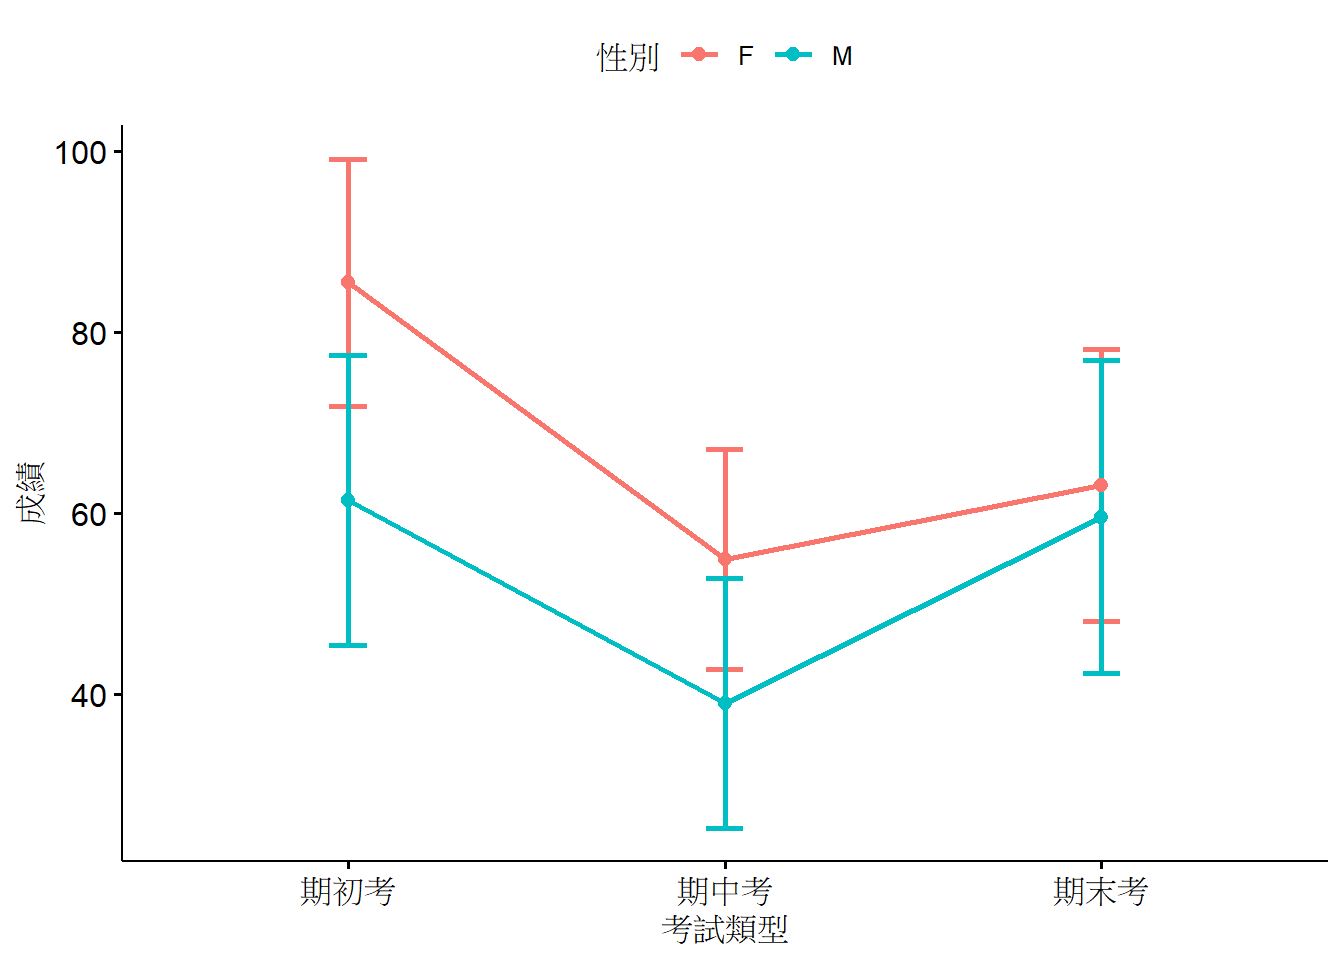
\includegraphics{quick-r-statistics_files/figure-latex/unnamed-chunk-95-1.pdf}

\hypertarget{ux8b8aux7570ux6578ux5206ux6790-2}{%
\section{變異數分析}\label{ux8b8aux7570ux6578ux5206ux6790-2}}

先將編號和性別的格式改為factor。

\begin{Shaded}
\begin{Highlighting}[]
\NormalTok{gData2WAmim}\SpecialCharTok{$}\NormalTok{編號 }\OtherTok{\textless{}{-}} \FunctionTok{factor}\NormalTok{(gData2WAmim}\SpecialCharTok{$}\NormalTok{編號)}
\NormalTok{gData2WAmim}\SpecialCharTok{$}\NormalTok{性別 }\OtherTok{\textless{}{-}} \FunctionTok{factor}\NormalTok{(gData2WAmim}\SpecialCharTok{$}\NormalTok{性別)}
\FunctionTok{str}\NormalTok{(gData2WAmim)}
\end{Highlighting}
\end{Shaded}

\begin{verbatim}
## 'data.frame':    162 obs. of  4 variables:
##  $ 編號    : Factor w/ 54 levels "1","2","3","4",..: 1 2 3 4 5 6 7 8 9 10 ...
##  $ 性別    : Factor w/ 2 levels "F","M": 2 2 1 1 2 1 1 1 2 2 ...
##  $ 考試類型: Factor w/ 3 levels "期初考","期中考",..: 1 1 1 1 1 1 1 1 1 1 ...
##  $ 成績    : num  46 54 64 64 74 96 40 96 74 66 ...
\end{verbatim}

用levene\_test()做變異數同質性檢定。預設值是center=median,如有需要可改為center=mean。分析結果可知,無論是何種考試類型,成績在不同性別上都不違反變異數同質性假設。

\begin{Shaded}
\begin{Highlighting}[]
\FunctionTok{levene\_test}\NormalTok{(}\FunctionTok{group\_by}\NormalTok{(gData2WAmim, 考試類型), 成績 }\SpecialCharTok{\textasciitilde{}}\NormalTok{ 性別)}
\end{Highlighting}
\end{Shaded}

\begin{verbatim}
## # A tibble: 3 x 5
##   考試類型   df1   df2 statistic     p
##   <fct>    <int> <int>     <dbl> <dbl>
## 1 期初考       1    52     0.239 0.627
## 2 期中考       1    52     0.156 0.695
## 3 期末考       1    52     0.273 0.604
\end{verbatim}

用rstatix package中的anova\_test()來做球型檢定和變異數分析,將結果儲存為res.aov。並以res.aov來看檢驗的結果。

因本資料違反球型假設,需要看sphericity correction的表。Sphericity Corrections以Greenhouse-Geisser (GG)和Huynh-Feldt (HF) epsilon values來做校正。校正後的值 p{[}GG{]} 和 p{[}HF{]} 皆小於.001,表示不同考試類型的成績有顯著差異,且存在性別與考試類型的交互作用。

\begin{Shaded}
\begin{Highlighting}[]
\FunctionTok{library}\NormalTok{(rstatix)}
\NormalTok{res.aov }\OtherTok{\textless{}{-}} \FunctionTok{anova\_test}\NormalTok{(}\AttributeTok{data =}\NormalTok{ gData2WAmim, }\AttributeTok{dv =}\NormalTok{ 成績, }\AttributeTok{wid =}\NormalTok{ 編號, }\AttributeTok{between =}\NormalTok{ 性別, }\AttributeTok{within =}\NormalTok{ 考試類型)}
\NormalTok{res.aov}
\end{Highlighting}
\end{Shaded}

\begin{verbatim}
## ANOVA Table (type II tests)
## 
## $ANOVA
##          Effect DFn DFd      F        p p<.05   ges
## 1          性別   1  52 22.604 1.62e-05     * 0.200
## 2      考試類型   2 104 68.691 9.66e-20     * 0.359
## 3 性別:考試類型   2 104 10.420 7.51e-05     * 0.078
## 
## $`Mauchly's Test for Sphericity`
##          Effect     W     p p<.05
## 1      考試類型 0.817 0.006     *
## 2 性別:考試類型 0.817 0.006     *
## 
## $`Sphericity Corrections`
##          Effect   GGe      DF[GG]    p[GG] p[GG]<.05   HFe      DF[HF]    p[HF]
## 1      考試類型 0.846 1.69, 87.94 4.53e-17         * 0.871 1.74, 90.57 1.65e-17
## 2 性別:考試類型 0.846 1.69, 87.94 2.11e-04         * 0.871 1.74, 90.57 1.78e-04
##   p[HF]<.05
## 1         *
## 2         *
\end{verbatim}

最後,用get\_anova\_table()來看校正後的結果。校正的結果顯示,性別主效果顯著,F(1, 52) = 22.6, p \textless{} .001;考試類型主效果顯著,F(1.69, 87.94) = 68.7, p \textless{} .001;兩變項的交互作用顯著,F(1.69, 87.94) = 10.4, p \textless{} .001。

\begin{Shaded}
\begin{Highlighting}[]
\FunctionTok{get\_anova\_table}\NormalTok{(res.aov)}
\end{Highlighting}
\end{Shaded}

\begin{verbatim}
## ANOVA Table (type II tests)
## 
##          Effect  DFn   DFd      F        p p<.05   ges
## 1          性別 1.00 52.00 22.604 1.62e-05     * 0.200
## 2      考試類型 1.69 87.94 68.691 4.53e-17     * 0.359
## 3 性別:考試類型 1.69 87.94 10.420 2.11e-04     * 0.078
\end{verbatim}

\hypertarget{ux4e8bux5f8cux6bd4ux8f03-1}{%
\subsection{事後比較}\label{ux4e8bux5f8cux6bd4ux8f03-1}}

交互作用顯著時的單純主要效果檢驗
因交互作用顯著,故需分析單純主要效果。先依考試類型來分組,看性別的主要效果。可知男女在期初考和期考成績有差異,在期末考則無。adjust\_pvalue()會考慮alpha值膨脹的問題,在控制三個檢定的alpha值不超過.05來計算p value。

\begin{Shaded}
\begin{Highlighting}[]
\NormalTok{anova1 }\OtherTok{\textless{}{-}} \FunctionTok{anova\_test}\NormalTok{(}\FunctionTok{group\_by}\NormalTok{(gData2WAmim, 考試類型), }\AttributeTok{dv=}\NormalTok{成績, }\AttributeTok{wid=}\NormalTok{編號, }\AttributeTok{between=}\NormalTok{性別)}
\FunctionTok{adjust\_pvalue}\NormalTok{(}\FunctionTok{get\_anova\_table}\NormalTok{(anova1), }\AttributeTok{method=}\StringTok{"bonferroni"}\NormalTok{)}
\end{Highlighting}
\end{Shaded}

\begin{verbatim}
## # A tibble: 3 x 9
##   考試類型 Effect   DFn   DFd      F           p `p<.05`   ges       p.adj
##   <fct>    <chr>  <dbl> <dbl>  <dbl>       <dbl> <chr>   <dbl>       <dbl>
## 1 期初考   性別       1    52 35.2   0.000000243 "*"     0.404 0.000000729
## 2 期中考   性別       1    52 20.2   0.0000398   "*"     0.279 0.000119   
## 3 期末考   性別       1    52  0.636 0.429       ""      0.012 1
\end{verbatim}

依性別來分組,看考試類型的主要效果。可知考試類型在男女上皆有差異。

\begin{Shaded}
\begin{Highlighting}[]
\NormalTok{anova2 }\OtherTok{\textless{}{-}} \FunctionTok{anova\_test}\NormalTok{(}\FunctionTok{group\_by}\NormalTok{(gData2WAmim, 性別), }\AttributeTok{dv=}\NormalTok{成績, }\AttributeTok{wid=}\NormalTok{編號, }\AttributeTok{within=}\NormalTok{考試類型)}
\FunctionTok{adjust\_pvalue}\NormalTok{(}\FunctionTok{get\_anova\_table}\NormalTok{(anova2), }\AttributeTok{method =} \StringTok{"bonferroni"}\NormalTok{)}
\end{Highlighting}
\end{Shaded}

\begin{verbatim}
## # A tibble: 2 x 9
##   性別  Effect     DFn   DFd     F        p `p<.05`   ges    p.adj
##   <fct> <chr>    <dbl> <dbl> <dbl>    <dbl> <chr>   <dbl>    <dbl>
## 1 F     考試類型     2    52  43.6 7.63e-12 *       0.482 1.53e-11
## 2 M     考試類型     2    52  34.4 3.03e-10 *       0.301 6.06e-10
\end{verbatim}

進一步以兩兩比較去看兩個主效果的差異在哪裡。結果顯示,女生無論是期初vs.期中、期初vs.期末、期vs.期末都有差異;男生則只有期初vs.期中、期中vs.期末有差異。

\begin{Shaded}
\begin{Highlighting}[]
\FunctionTok{pairwise\_t\_test}\NormalTok{(}\FunctionTok{group\_by}\NormalTok{(gData2WAmim,性別), 成績 }\SpecialCharTok{\textasciitilde{}}\NormalTok{ 考試類型, }\AttributeTok{paired =} \ConstantTok{TRUE}\NormalTok{, }\AttributeTok{p.adjust.method =} \StringTok{"bonferroni"}\NormalTok{)}
\end{Highlighting}
\end{Shaded}

\begin{verbatim}
## # A tibble: 6 x 11
##   性別  .y.   group1 group2    n1    n2 statistic    df             p      p.adj
## * <fct> <chr> <chr>  <chr>  <int> <int>     <dbl> <dbl>         <dbl>      <dbl>
## 1 F     成績  期初考 期中考    27    27     8.73     26 0.00000000334    1   e-8
## 2 F     成績  期初考 期末考    27    27     5.72     26 0.00000506       1.52e-5
## 3 F     成績  期中考 期末考    27    27    -3.13     26 0.004            1.3 e-2
## 4 M     成績  期初考 期中考    27    27     6.67     26 0.000000447      1.34e-6
## 5 M     成績  期初考 期末考    27    27     0.557    26 0.582            1   e+0
## 6 M     成績  期中考 期末考    27    27    -9.27     26 0.000000001      3   e-9
## # ... with 1 more variable: p.adj.signif <chr>
\end{verbatim}

\hypertarget{ux4ea4ux4e92ux4f5cux7528ux672aux986fux8457ux6642ux7684ux4e8bux5f8cux6bd4ux8f03}{%
\subsection{交互作用未顯著時的事後比較}\label{ux4ea4ux4e92ux4f5cux7528ux672aux986fux8457ux6642ux7684ux4e8bux5f8cux6bd4ux8f03}}

若交互作用未顯著,看主效果的事後比較。因性別只有兩個levels,不需進行事後比較。因此看考試類型的兩兩比較,結果顯示,三種考試的成績兩兩之間都有差異。

\begin{Shaded}
\begin{Highlighting}[]
\FunctionTok{pairwise\_t\_test}\NormalTok{(gData2WAmim, 成績}\SpecialCharTok{\textasciitilde{}}\NormalTok{考試類型, }\AttributeTok{paired =} \ConstantTok{TRUE}\NormalTok{, }\AttributeTok{p.adjust.method =} \StringTok{"bonferroni"}\NormalTok{)}
\end{Highlighting}
\end{Shaded}

\begin{verbatim}
## # A tibble: 3 x 10
##   .y.   group1 group2    n1    n2 statistic    df        p    p.adj p.adj.signif
## * <chr> <chr>  <chr>  <int> <int>     <dbl> <dbl>    <dbl>    <dbl> <chr>       
## 1 成績  期初考 期中考    54    54     10.7     53 6.73e-15 2.02e-14 ****        
## 2 成績  期初考 期末考    54    54      4.18    53 1.1 e- 4 3.3 e- 4 ***         
## 3 成績  期中考 期末考    54    54     -7.56    53 5.6 e-10 1.68e- 9 ****
\end{verbatim}

\hypertarget{multireg}{%
\chapter{多元迴歸}\label{multireg}}

以R語言內建的mtcars做多元迴歸。

\hypertarget{ux8cc7ux6599ux7684ux6e96ux5099ux8207ux6aa2ux8996}{%
\section{資料的準備與檢視}\label{ux8cc7ux6599ux7684ux6e96ux5099ux8207ux6aa2ux8996}}

\hypertarget{ux8b80ux5165ux6a94ux6848-6}{%
\subsection{讀入檔案}\label{ux8b80ux5165ux6a94ux6848-6}}

讀入mtcars檔案。mtcars是R內建的dataset,為1974年美國的Motor Trend雜誌對32種車款在11項設計與表現所做的整理,包含油耗量(mpg)、氣缸數(cyl)、排氣量(disp)、馬力(hp)、車體重量(wt)、加速時間(qsec)等。

\begin{Shaded}
\begin{Highlighting}[]
\FunctionTok{data}\NormalTok{(mtcars)}
\FunctionTok{head}\NormalTok{(mtcars, }\DecValTok{10}\NormalTok{)}
\end{Highlighting}
\end{Shaded}

\begin{verbatim}
##                    mpg cyl  disp  hp drat    wt  qsec vs am gear carb
## Mazda RX4         21.0   6 160.0 110 3.90 2.620 16.46  0  1    4    4
## Mazda RX4 Wag     21.0   6 160.0 110 3.90 2.875 17.02  0  1    4    4
## Datsun 710        22.8   4 108.0  93 3.85 2.320 18.61  1  1    4    1
## Hornet 4 Drive    21.4   6 258.0 110 3.08 3.215 19.44  1  0    3    1
## Hornet Sportabout 18.7   8 360.0 175 3.15 3.440 17.02  0  0    3    2
## Valiant           18.1   6 225.0 105 2.76 3.460 20.22  1  0    3    1
## Duster 360        14.3   8 360.0 245 3.21 3.570 15.84  0  0    3    4
## Merc 240D         24.4   4 146.7  62 3.69 3.190 20.00  1  0    4    2
## Merc 230          22.8   4 140.8  95 3.92 3.150 22.90  1  0    4    2
## Merc 280          19.2   6 167.6 123 3.92 3.440 18.30  1  0    4    4
\end{verbatim}

\hypertarget{ux6aa2ux8996ux76f8ux95dc}{%
\subsection{檢視相關}\label{ux6aa2ux8996ux76f8ux95dc}}

先用plot()看各變項的關鍵性。

\begin{Shaded}
\begin{Highlighting}[]
\FunctionTok{plot}\NormalTok{(mtcars[}\DecValTok{1}\SpecialCharTok{:}\DecValTok{7}\NormalTok{])}
\end{Highlighting}
\end{Shaded}

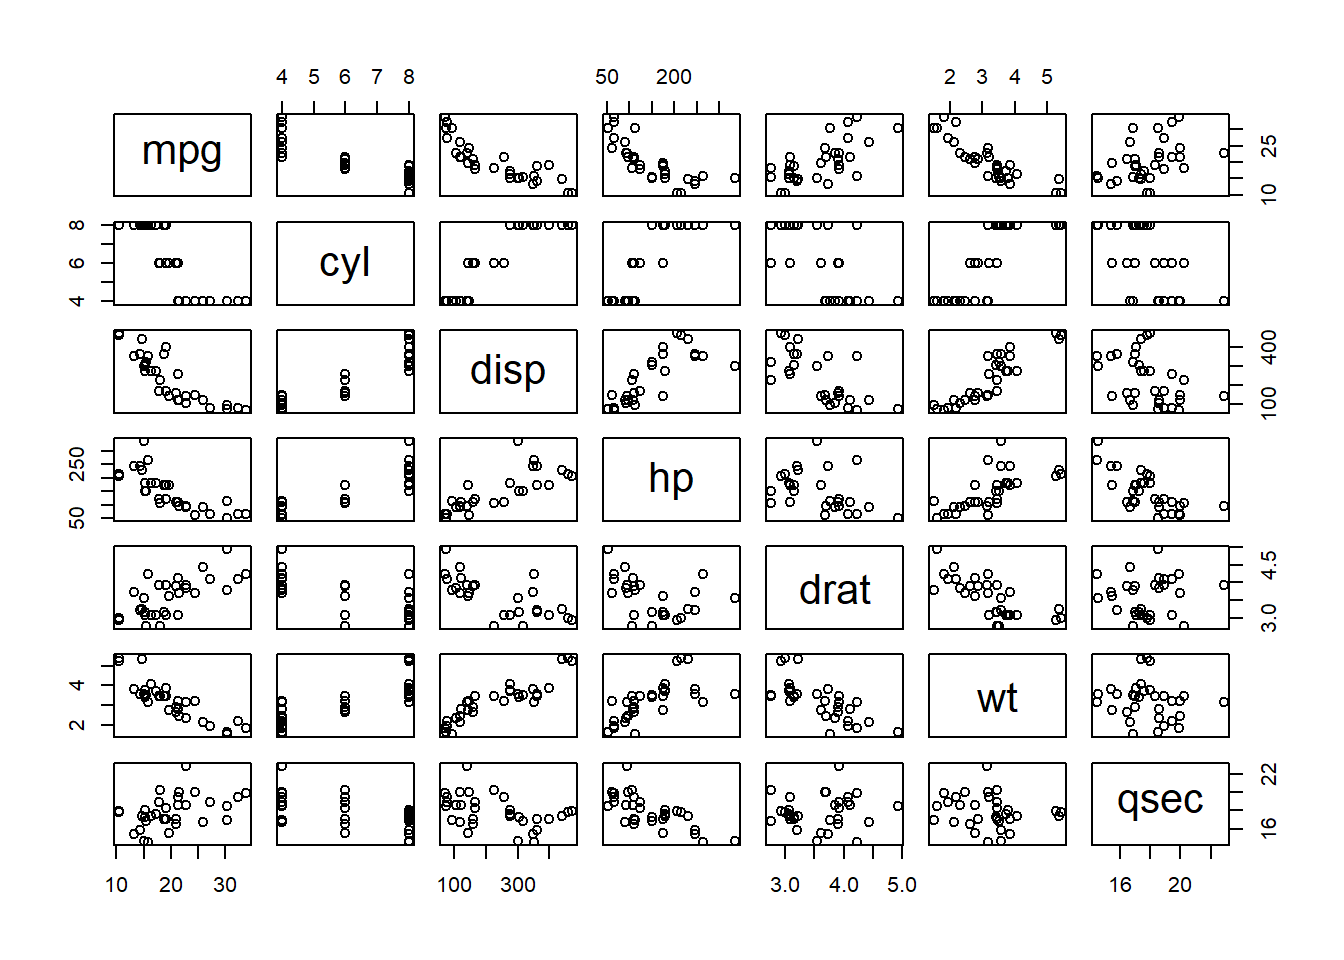
\includegraphics{quick-r-statistics_files/figure-latex/unnamed-chunk-105-1.pdf}

計算各變項的相關。

\begin{Shaded}
\begin{Highlighting}[]
\FunctionTok{library}\NormalTok{(Hmisc)}
\FunctionTok{rcorr}\NormalTok{(}\FunctionTok{data.matrix}\NormalTok{(mtcars[}\DecValTok{1}\SpecialCharTok{:}\DecValTok{7}\NormalTok{]))}
\end{Highlighting}
\end{Shaded}

\begin{verbatim}
##        mpg   cyl  disp    hp  drat    wt  qsec
## mpg   1.00 -0.85 -0.85 -0.78  0.68 -0.87  0.42
## cyl  -0.85  1.00  0.90  0.83 -0.70  0.78 -0.59
## disp -0.85  0.90  1.00  0.79 -0.71  0.89 -0.43
## hp   -0.78  0.83  0.79  1.00 -0.45  0.66 -0.71
## drat  0.68 -0.70 -0.71 -0.45  1.00 -0.71  0.09
## wt   -0.87  0.78  0.89  0.66 -0.71  1.00 -0.17
## qsec  0.42 -0.59 -0.43 -0.71  0.09 -0.17  1.00
## 
## n= 32 
## 
## 
## P
##      mpg    cyl    disp   hp     drat   wt     qsec  
## mpg         0.0000 0.0000 0.0000 0.0000 0.0000 0.0171
## cyl  0.0000        0.0000 0.0000 0.0000 0.0000 0.0004
## disp 0.0000 0.0000        0.0000 0.0000 0.0000 0.0131
## hp   0.0000 0.0000 0.0000        0.0100 0.0000 0.0000
## drat 0.0000 0.0000 0.0000 0.0100        0.0000 0.6196
## wt   0.0000 0.0000 0.0000 0.0000 0.0000        0.3389
## qsec 0.0171 0.0004 0.0131 0.0000 0.6196 0.3389
\end{verbatim}

\hypertarget{ux8ff4ux6b78ux5206ux6790}{%
\section{迴歸分析}\label{ux8ff4ux6b78ux5206ux6790}}

\hypertarget{ux7c21ux55aeux8ff4ux6b78}{%
\subsection{簡單迴歸}\label{ux7c21ux55aeux8ff4ux6b78}}

以lm()檢驗是否可以用車體重量(wt)預測油耗量(mpg)。結果顯示R-square = 0.75,F(1,30) = 91.38,p\textless.001,F檢定顯著,模型有良好解釋力。迴歸式為 mpg = -5.3445*wt + 37.2851。

\begin{Shaded}
\begin{Highlighting}[]
\NormalTok{model.mpg.wt }\OtherTok{\textless{}{-}} \FunctionTok{lm}\NormalTok{(mpg }\SpecialCharTok{\textasciitilde{}}\NormalTok{ wt, }\AttributeTok{data =}\NormalTok{ mtcars)}
\FunctionTok{summary}\NormalTok{(model.mpg.wt)}
\end{Highlighting}
\end{Shaded}

\begin{verbatim}
## 
## Call:
## lm(formula = mpg ~ wt, data = mtcars)
## 
## Residuals:
##     Min      1Q  Median      3Q     Max 
## -4.5432 -2.3647 -0.1252  1.4096  6.8727 
## 
## Coefficients:
##             Estimate Std. Error t value Pr(>|t|)    
## (Intercept)  37.2851     1.8776  19.858  < 2e-16 ***
## wt           -5.3445     0.5591  -9.559 1.29e-10 ***
## ---
## Signif. codes:  0 '***' 0.001 '**' 0.01 '*' 0.05 '.' 0.1 ' ' 1
## 
## Residual standard error: 3.046 on 30 degrees of freedom
## Multiple R-squared:  0.7528, Adjusted R-squared:  0.7446 
## F-statistic: 91.38 on 1 and 30 DF,  p-value: 1.294e-10
\end{verbatim}

以package visreg的visreg()函數來畫迴歸線。

\begin{Shaded}
\begin{Highlighting}[]
\FunctionTok{library}\NormalTok{(visreg)}
\FunctionTok{visreg}\NormalTok{(model.mpg.wt)}
\end{Highlighting}
\end{Shaded}

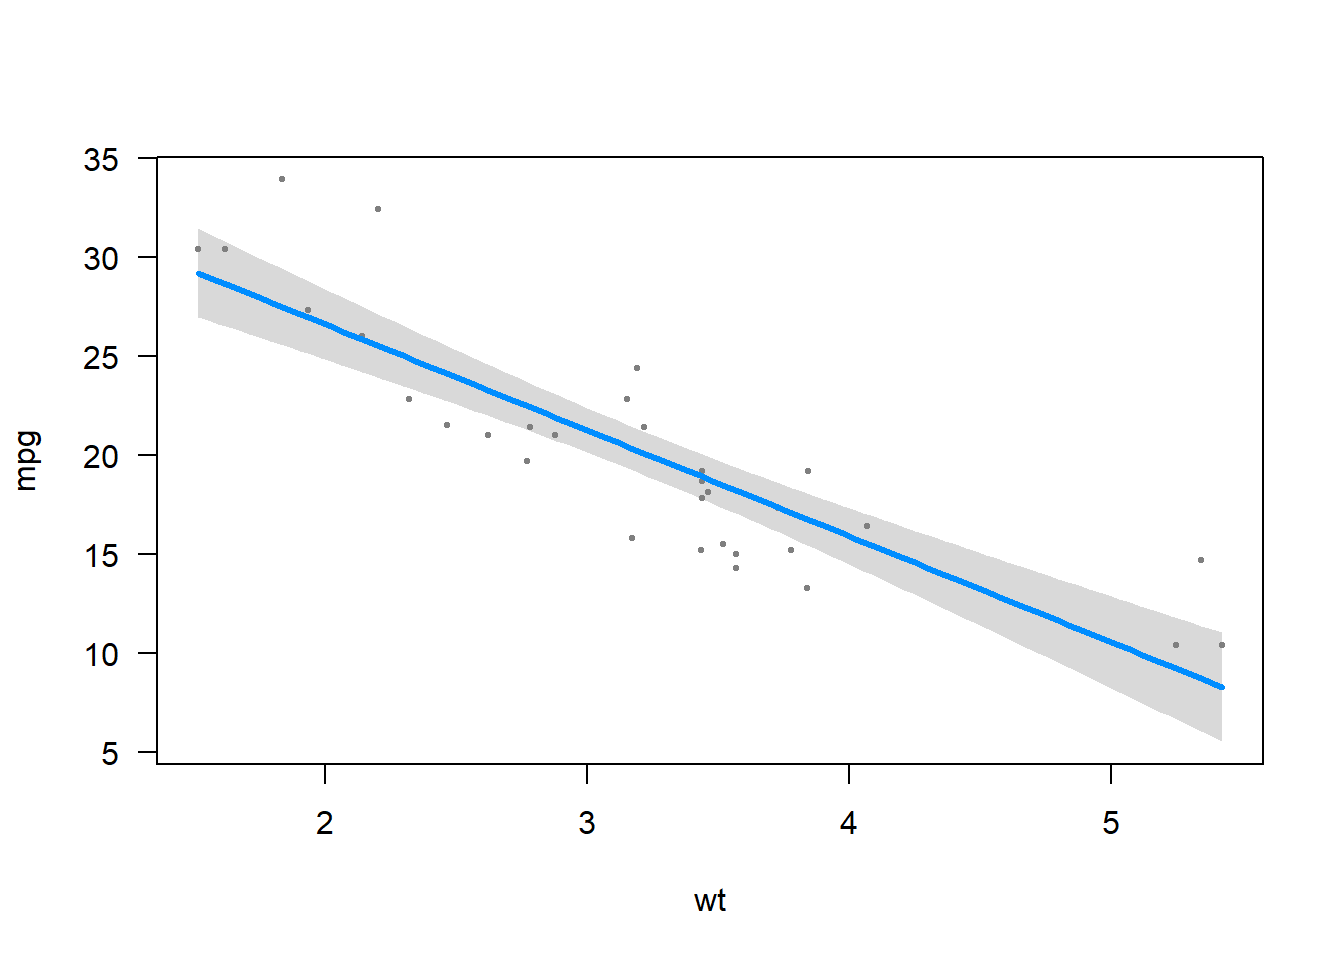
\includegraphics{quick-r-statistics_files/figure-latex/unnamed-chunk-108-1.pdf}

\hypertarget{ux591aux5143ux8ff4ux6b78}{%
\subsection{多元迴歸}\label{ux591aux5143ux8ff4ux6b78}}

以車體重量(wt)、馬力(hp)和排氣量(disp)來預測油耗量(mpg)。相關分析顯示三個預測項與油耗量皆為負相關。

以lm()來做迴歸分析,迴歸分析結果顯示,R-square = 0.8268,F(3,28) = 44.57, p \textless{} .01。disp沒有顯著。

\begin{Shaded}
\begin{Highlighting}[]
\NormalTok{model.mpg.whd }\OtherTok{\textless{}{-}} \FunctionTok{update}\NormalTok{(model.mpg.wt, .}\SpecialCharTok{\textasciitilde{}}\NormalTok{. }\SpecialCharTok{+}\NormalTok{ hp }\SpecialCharTok{+}\NormalTok{ disp, }\AttributeTok{data=}\NormalTok{mtcars)}
\NormalTok{model.mpg.whd }\OtherTok{\textless{}{-}} \FunctionTok{lm}\NormalTok{(mpg }\SpecialCharTok{\textasciitilde{}}\NormalTok{ wt }\SpecialCharTok{+}\NormalTok{ hp }\SpecialCharTok{+}\NormalTok{ disp, }\AttributeTok{data =}\NormalTok{ mtcars)}
\FunctionTok{summary}\NormalTok{(model.mpg.whd)}
\end{Highlighting}
\end{Shaded}

\begin{verbatim}
## 
## Call:
## lm(formula = mpg ~ wt + hp + disp, data = mtcars)
## 
## Residuals:
##    Min     1Q Median     3Q    Max 
## -3.891 -1.640 -0.172  1.061  5.861 
## 
## Coefficients:
##              Estimate Std. Error t value Pr(>|t|)    
## (Intercept) 37.105505   2.110815  17.579  < 2e-16 ***
## wt          -3.800891   1.066191  -3.565  0.00133 ** 
## hp          -0.031157   0.011436  -2.724  0.01097 *  
## disp        -0.000937   0.010350  -0.091  0.92851    
## ---
## Signif. codes:  0 '***' 0.001 '**' 0.01 '*' 0.05 '.' 0.1 ' ' 1
## 
## Residual standard error: 2.639 on 28 degrees of freedom
## Multiple R-squared:  0.8268, Adjusted R-squared:  0.8083 
## F-statistic: 44.57 on 3 and 28 DF,  p-value: 8.65e-11
\end{verbatim}

若想進一步看淨相關和半淨相關,可用pcor()做淨相關(partial correlation)、用spcor()做半淨相關(semi-partial correlation)。淨相關結果顯示,三變項皆顯著相關,all ps \textless{} .05。

\begin{Shaded}
\begin{Highlighting}[]
\FunctionTok{library}\NormalTok{(ppcor)}
\FunctionTok{round}\NormalTok{(}\FunctionTok{pcor}\NormalTok{(mtcars[}\FunctionTok{c}\NormalTok{(}\DecValTok{1}\NormalTok{,}\DecValTok{6}\NormalTok{,}\DecValTok{4}\NormalTok{,}\DecValTok{3}\NormalTok{)])}\SpecialCharTok{$}\NormalTok{estimate, }\DecValTok{03}\NormalTok{) }\CommentTok{\#partial}
\end{Highlighting}
\end{Shaded}

\begin{verbatim}
##         mpg     wt     hp   disp
## mpg   1.000 -0.559 -0.458 -0.017
## wt   -0.559  1.000 -0.370  0.651
## hp   -0.458 -0.370  1.000  0.521
## disp -0.017  0.651  0.521  1.000
\end{verbatim}

\begin{Shaded}
\begin{Highlighting}[]
\FunctionTok{round}\NormalTok{(}\FunctionTok{pcor}\NormalTok{(mtcars[}\FunctionTok{c}\NormalTok{(}\DecValTok{1}\NormalTok{,}\DecValTok{6}\NormalTok{,}\DecValTok{4}\NormalTok{,}\DecValTok{3}\NormalTok{)])}\SpecialCharTok{$}\NormalTok{p.value, }\DecValTok{03}\NormalTok{)}
\end{Highlighting}
\end{Shaded}

\begin{verbatim}
##        mpg    wt    hp  disp
## mpg  0.000 0.001 0.011 0.929
## wt   0.001 0.000 0.044 0.000
## hp   0.011 0.044 0.000 0.003
## disp 0.929 0.000 0.003 0.000
\end{verbatim}

半淨相關結果顯示,僅wt顯著相關。

\begin{Shaded}
\begin{Highlighting}[]
\FunctionTok{round}\NormalTok{(}\FunctionTok{spcor}\NormalTok{(mtcars[}\FunctionTok{c}\NormalTok{(}\DecValTok{1}\NormalTok{,}\DecValTok{6}\NormalTok{,}\DecValTok{4}\NormalTok{,}\DecValTok{3}\NormalTok{)])}\SpecialCharTok{$}\NormalTok{estimate, }\DecValTok{03}\NormalTok{) }\CommentTok{\#semi{-}partial}
\end{Highlighting}
\end{Shaded}

\begin{verbatim}
##         mpg     wt     hp   disp
## mpg   1.000 -0.280 -0.214 -0.007
## wt   -0.254  1.000 -0.150  0.323
## hp   -0.277 -0.214  1.000  0.328
## disp -0.006  0.317  0.226  1.000
\end{verbatim}

\begin{Shaded}
\begin{Highlighting}[]
\FunctionTok{round}\NormalTok{(}\FunctionTok{spcor}\NormalTok{(mtcars[}\FunctionTok{c}\NormalTok{(}\DecValTok{1}\NormalTok{,}\DecValTok{6}\NormalTok{,}\DecValTok{4}\NormalTok{,}\DecValTok{3}\NormalTok{)])}\SpecialCharTok{$}\NormalTok{p.value, }\DecValTok{03}\NormalTok{)}
\end{Highlighting}
\end{Shaded}

\begin{verbatim}
##        mpg    wt    hp  disp
## mpg  0.000 0.133 0.256 0.970
## wt   0.176 0.000 0.429 0.081
## hp   0.139 0.256 0.000 0.076
## disp 0.974 0.088 0.230 0.000
\end{verbatim}

看各變項對mpg的關係。

\begin{Shaded}
\begin{Highlighting}[]
\FunctionTok{visreg}\NormalTok{(model.mpg.whd)}
\end{Highlighting}
\end{Shaded}

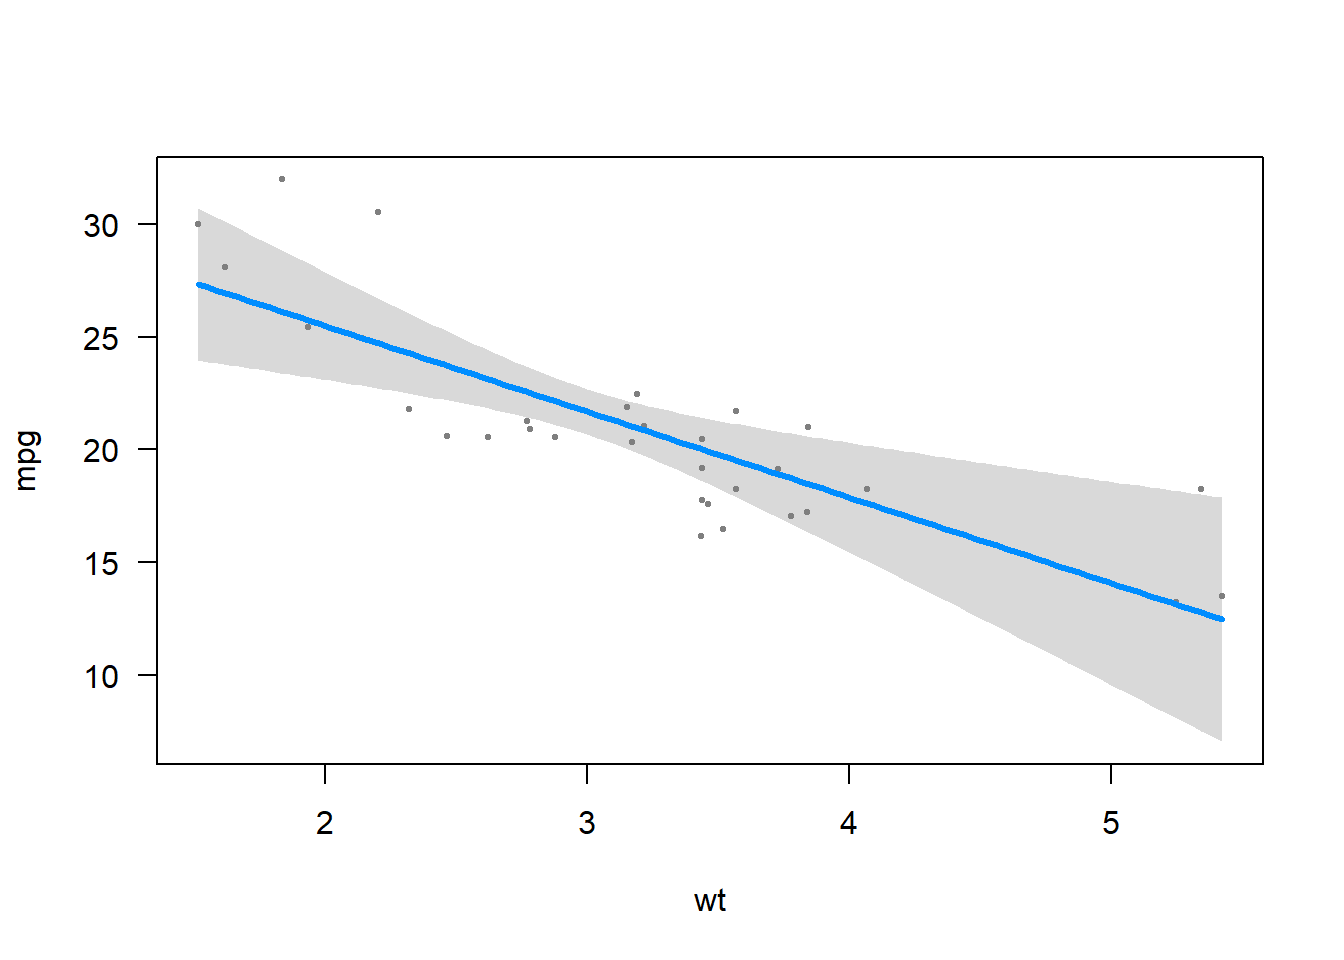
\includegraphics{quick-r-statistics_files/figure-latex/unnamed-chunk-112-1.pdf} 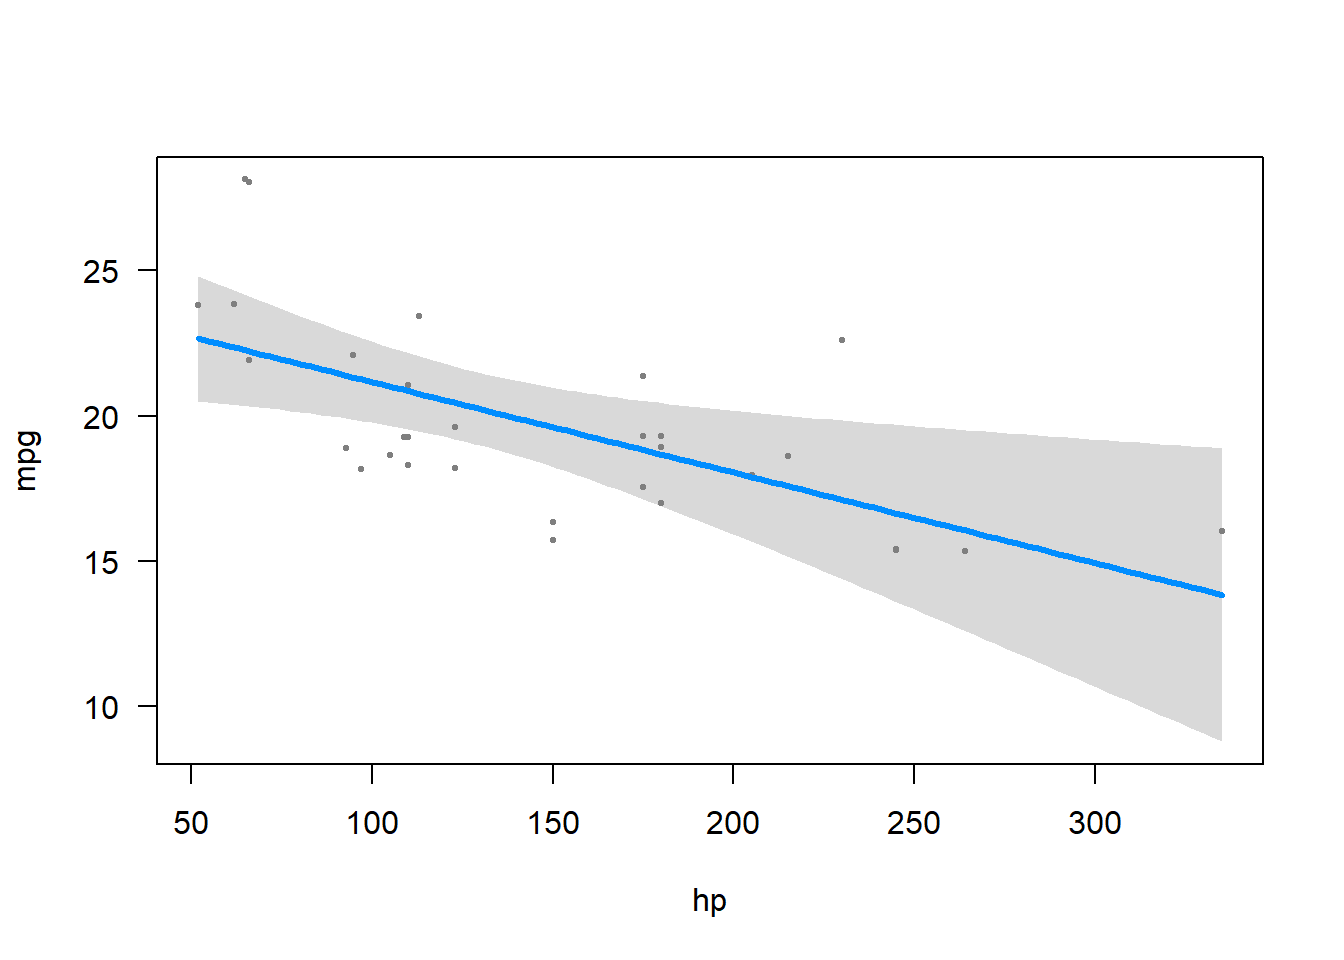
\includegraphics{quick-r-statistics_files/figure-latex/unnamed-chunk-112-2.pdf} 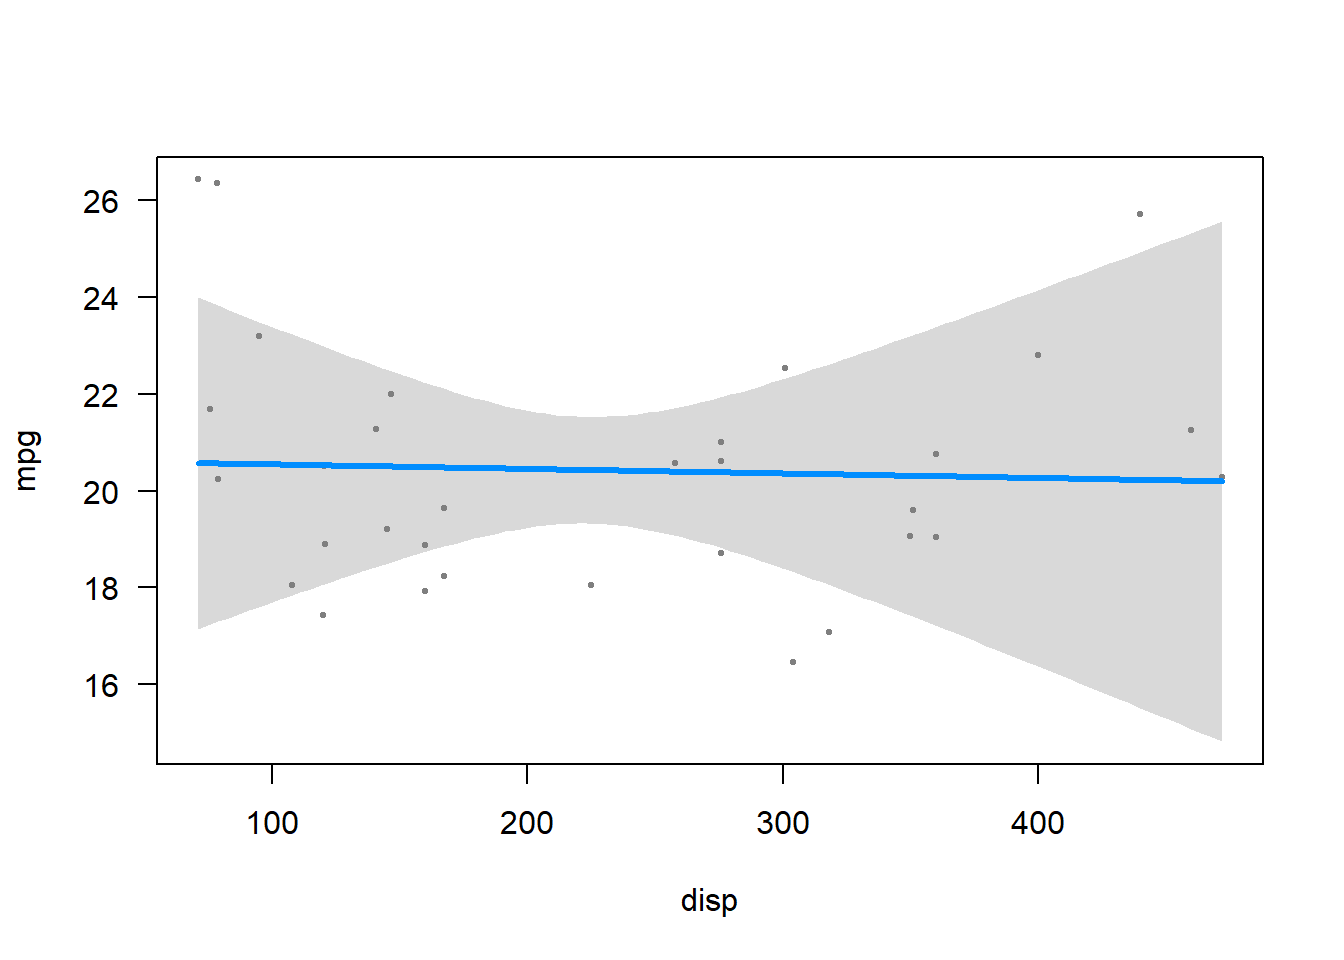
\includegraphics{quick-r-statistics_files/figure-latex/unnamed-chunk-112-3.pdf}

以predict()來做預測。

\begin{Shaded}
\begin{Highlighting}[]
\FunctionTok{predict}\NormalTok{(model.mpg.whd,}
        \AttributeTok{new =} \FunctionTok{data.frame}\NormalTok{(}\AttributeTok{wt =} \DecValTok{5}\NormalTok{, }\AttributeTok{hp =} \DecValTok{250}\NormalTok{, }\AttributeTok{disp =} \DecValTok{300}\NormalTok{, }\AttributeTok{am =} \StringTok{"Manual"}\NormalTok{),}
        \AttributeTok{interval =} \StringTok{"confidence"}\NormalTok{,}
        \AttributeTok{level =}\NormalTok{ .}\DecValTok{95}
\NormalTok{)}
\end{Highlighting}
\end{Shaded}

\begin{verbatim}
##        fit      lwr      upr
## 1 10.03081 6.335154 13.72647
\end{verbatim}

\hypertarget{ux8ff4ux6b78ux6a21ux578bux7684ux6bd4ux8f03}{%
\subsection{迴歸模型的比較}\label{ux8ff4ux6b78ux6a21ux578bux7684ux6bd4ux8f03}}

以ANOVA()來比較兩個迴歸模型。結果顯示三預測項的模型顯著優於一預測項模型。F(2, 83.33) = 5.98, p\textless.001。

\begin{Shaded}
\begin{Highlighting}[]
\FunctionTok{anova}\NormalTok{(model.mpg.wt, model.mpg.whd)}
\end{Highlighting}
\end{Shaded}

\begin{verbatim}
## Analysis of Variance Table
## 
## Model 1: mpg ~ wt
## Model 2: mpg ~ wt + hp + disp
##   Res.Df    RSS Df Sum of Sq     F   Pr(>F)   
## 1     30 278.32                               
## 2     28 194.99  2    83.331 5.983 0.006863 **
## ---
## Signif. codes:  0 '***' 0.001 '**' 0.01 '*' 0.05 '.' 0.1 ' ' 1
\end{verbatim}

用AIC()來看兩個模型的AIC(Akaike information criterion)。結果顯示相較於一個預測項時,以三個預測項來預測mpg時,AIC有下降。

\begin{Shaded}
\begin{Highlighting}[]
\FunctionTok{AIC}\NormalTok{(model.mpg.wt)}
\end{Highlighting}
\end{Shaded}

\begin{verbatim}
## [1] 166.0294
\end{verbatim}

\begin{Shaded}
\begin{Highlighting}[]
\FunctionTok{AIC}\NormalTok{(model.mpg.whd)}
\end{Highlighting}
\end{Shaded}

\begin{verbatim}
## [1] 158.643
\end{verbatim}

\hypertarget{ux8ff4ux6b78ux5047ux8a2dux7684ux6aa2ux9a57}{%
\section{迴歸假設的檢驗}\label{ux8ff4ux6b78ux5047ux8a2dux7684ux6aa2ux9a57}}

檢驗資料是否符合迴歸分析的假設。

\hypertarget{ux6975ux7aefux6578ux503cux7684ux5f71ux97ff}{%
\subsection{極端數值的影響}\label{ux6975ux7aefux6578ux503cux7684ux5f71ux97ff}}

standardize resuduals和studentize residuals。

\begin{Shaded}
\begin{Highlighting}[]
\FunctionTok{library}\NormalTok{(olsrr)}
\FunctionTok{ols\_plot\_resid\_stand}\NormalTok{(model.mpg.whd)}
\end{Highlighting}
\end{Shaded}

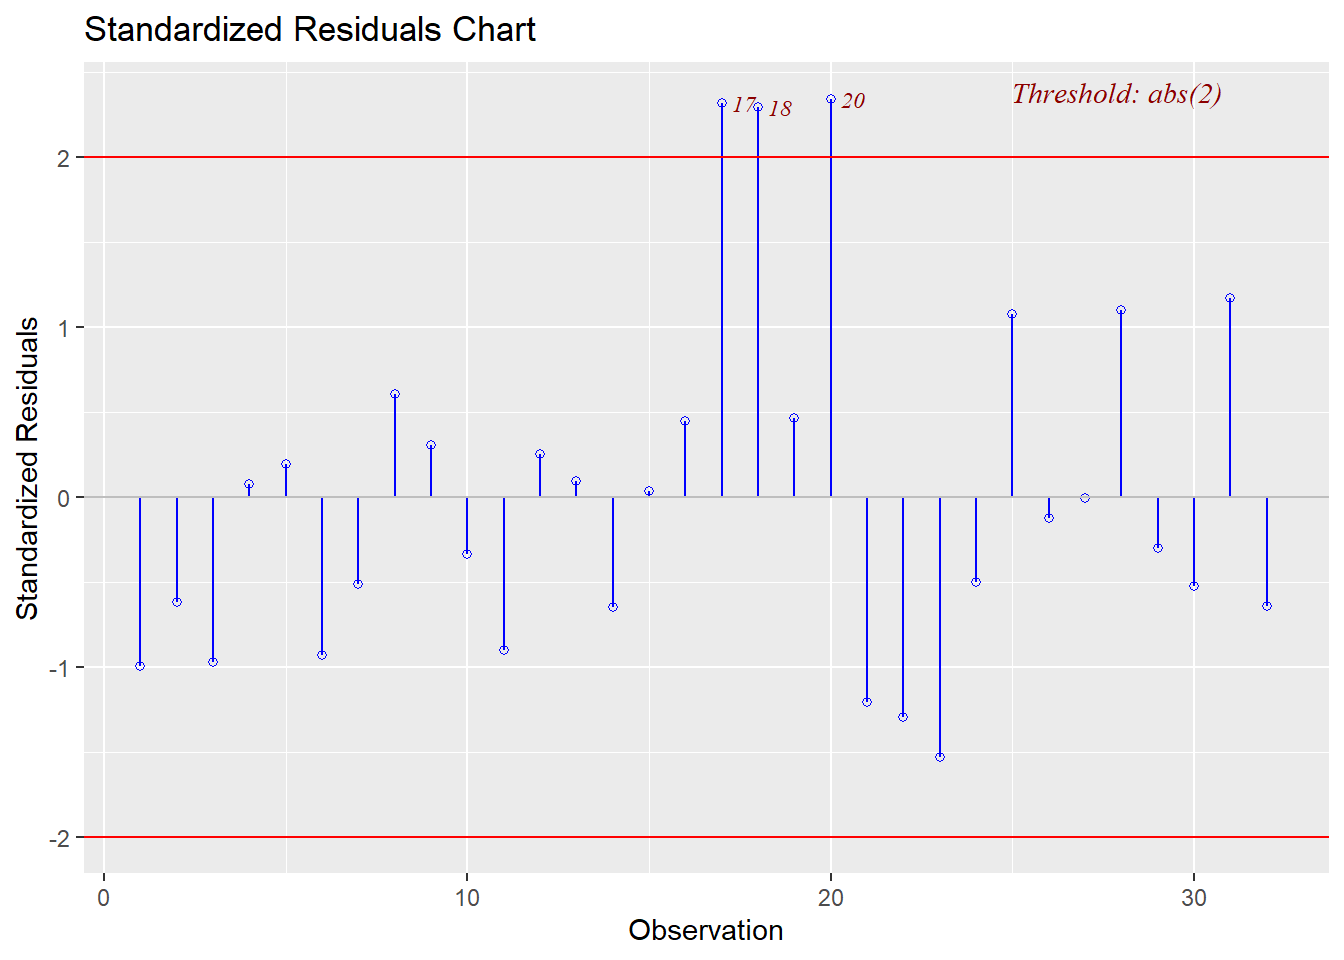
\includegraphics{quick-r-statistics_files/figure-latex/unnamed-chunk-117-1.pdf}

\begin{Shaded}
\begin{Highlighting}[]
\FunctionTok{ols\_plot\_resid\_stud}\NormalTok{(model.mpg.whd)}
\end{Highlighting}
\end{Shaded}

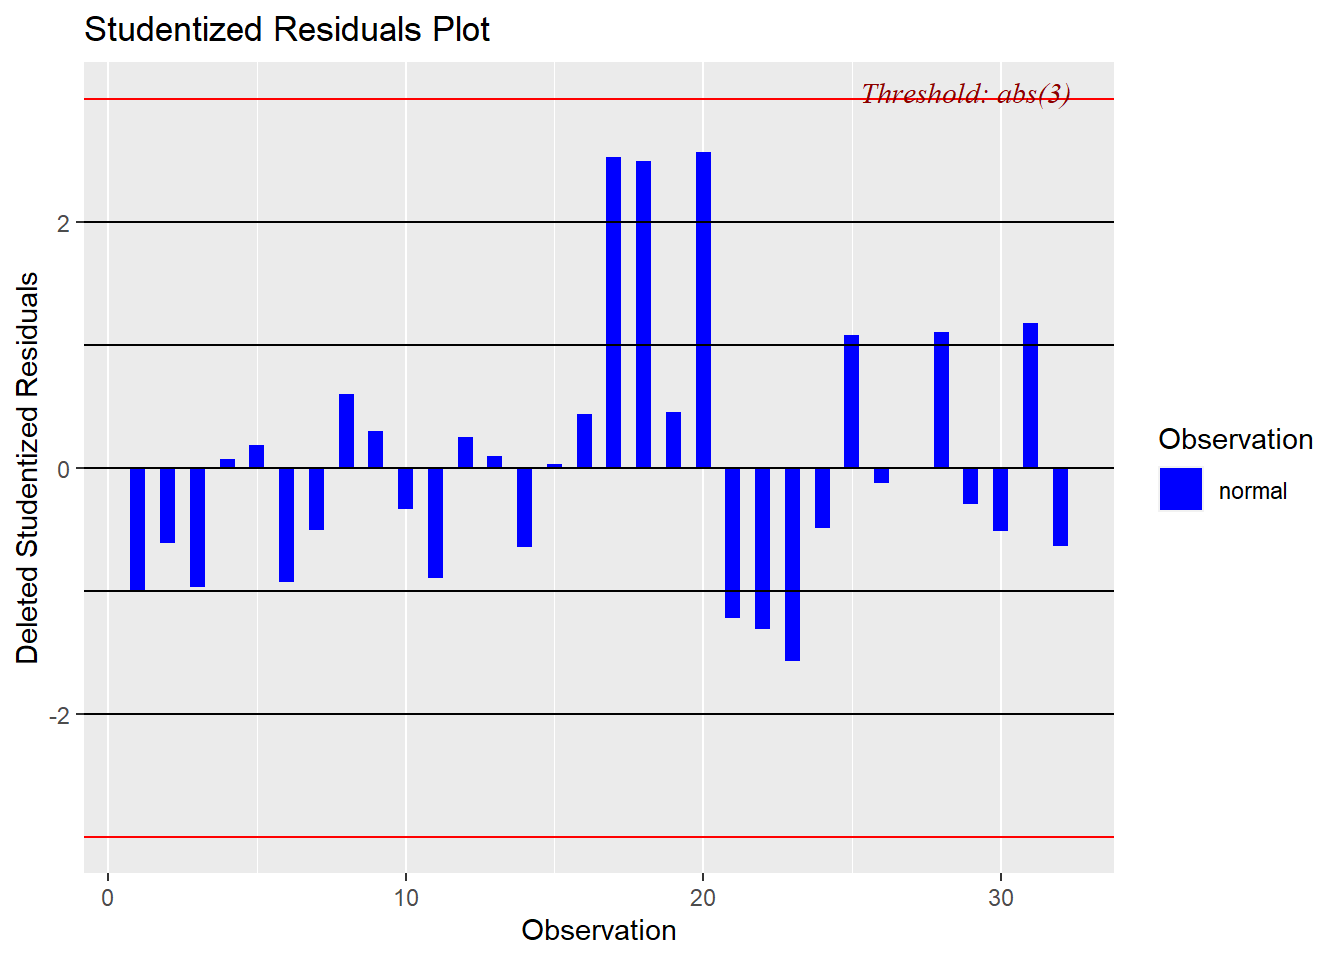
\includegraphics{quick-r-statistics_files/figure-latex/unnamed-chunk-118-1.pdf}

極端數值移除後對迴歸式的影響。

\begin{Shaded}
\begin{Highlighting}[]
\FunctionTok{ols\_plot\_dfbetas}\NormalTok{(model.mpg.whd)}
\end{Highlighting}
\end{Shaded}

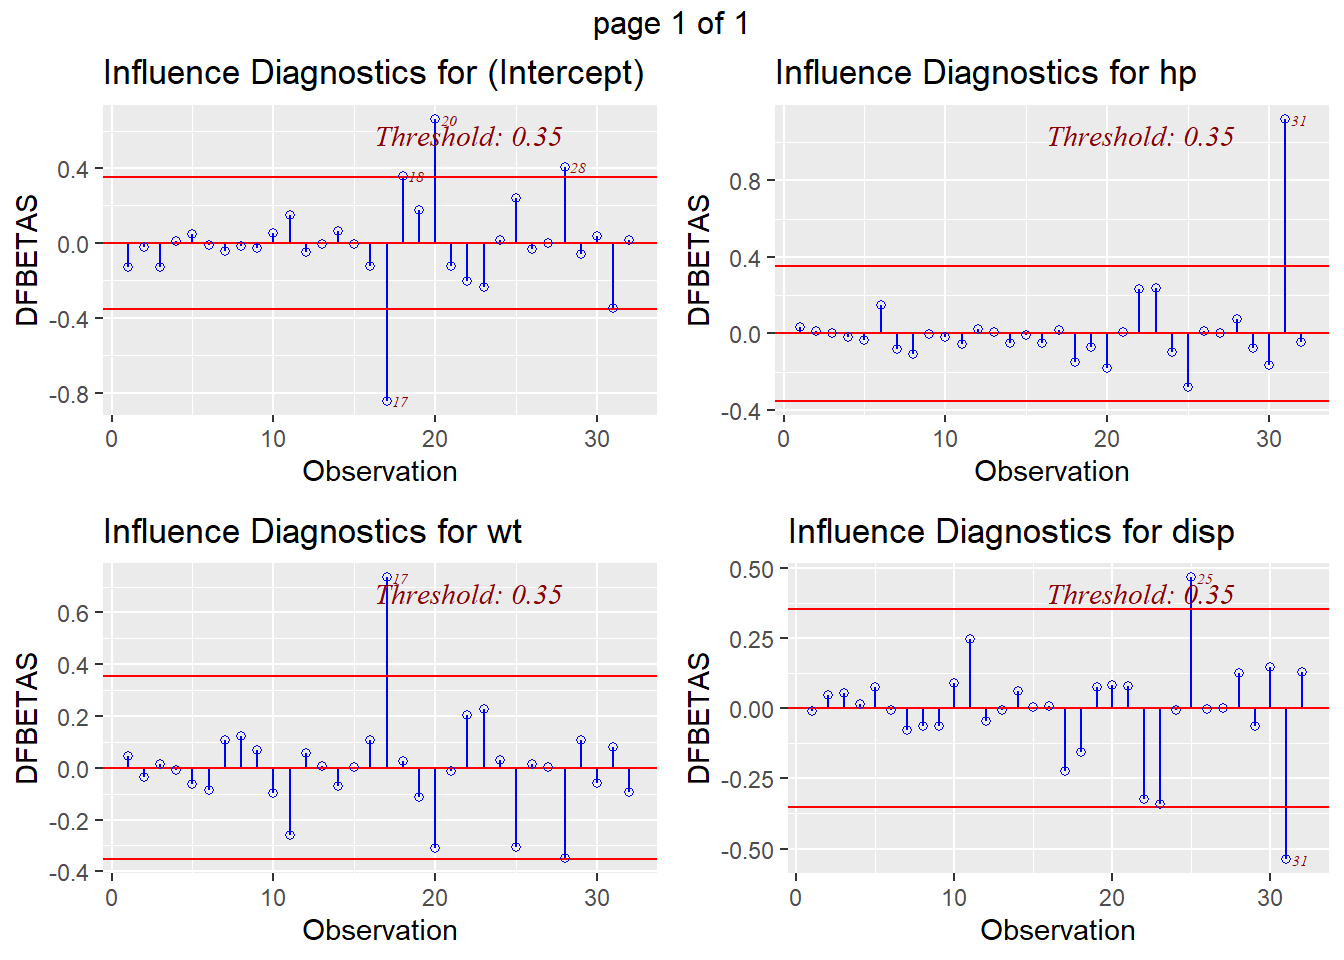
\includegraphics{quick-r-statistics_files/figure-latex/unnamed-chunk-119-1.pdf}

\begin{Shaded}
\begin{Highlighting}[]
\FunctionTok{ols\_plot\_dffits}\NormalTok{(model.mpg.whd)}
\end{Highlighting}
\end{Shaded}

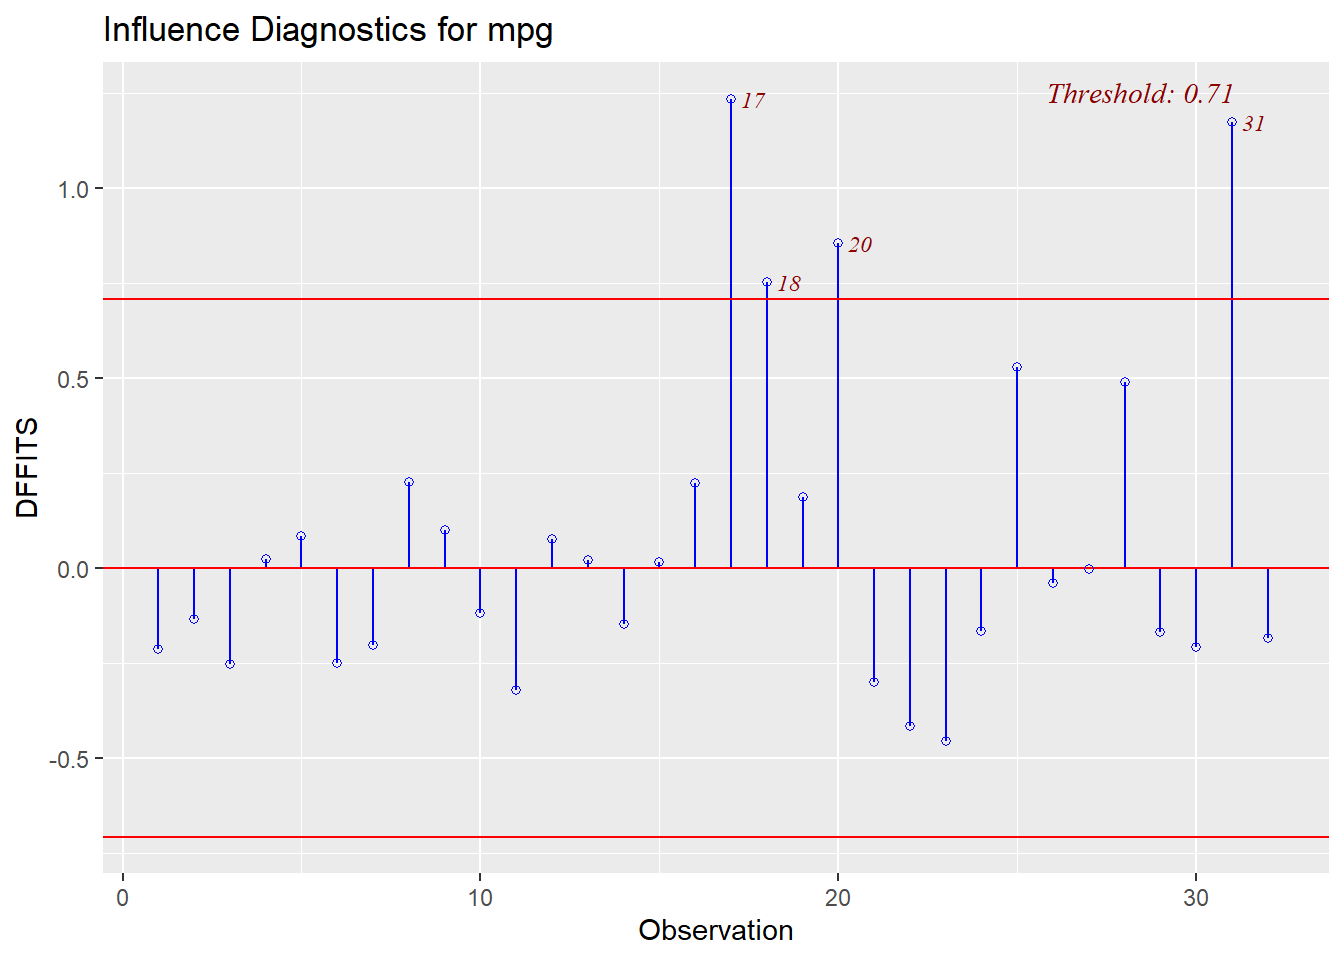
\includegraphics{quick-r-statistics_files/figure-latex/unnamed-chunk-120-1.pdf}

以Cook's distance看極端數值對整個模型的影響。

\begin{Shaded}
\begin{Highlighting}[]
\FunctionTok{ols\_plot\_cooksd\_bar}\NormalTok{(model.mpg.whd)}
\end{Highlighting}
\end{Shaded}

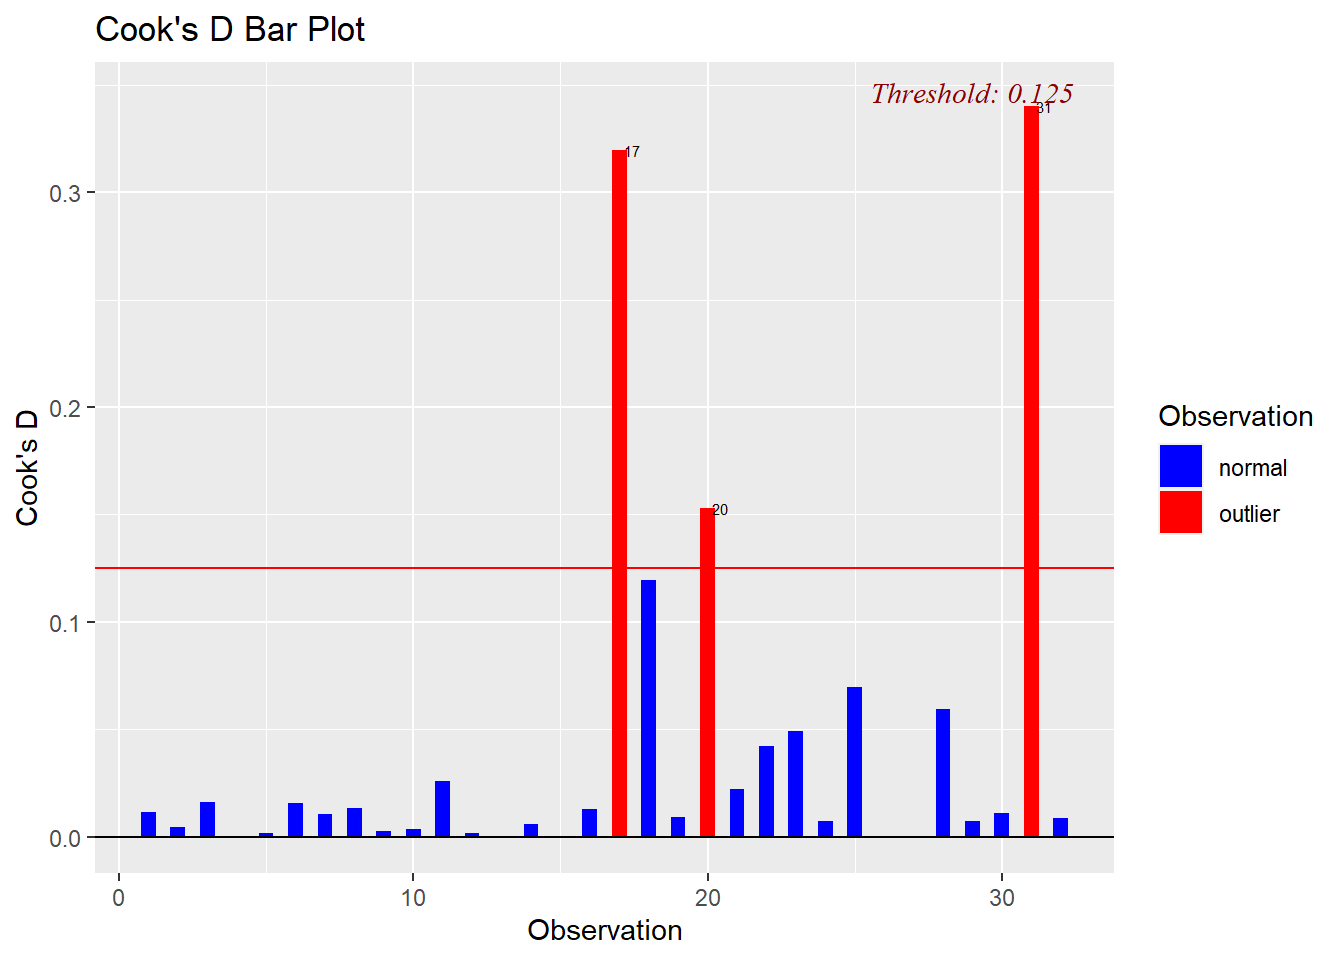
\includegraphics{quick-r-statistics_files/figure-latex/unnamed-chunk-121-1.pdf}

\begin{Shaded}
\begin{Highlighting}[]
\FunctionTok{ols\_plot\_cooksd\_chart}\NormalTok{(model.mpg.whd)}
\end{Highlighting}
\end{Shaded}

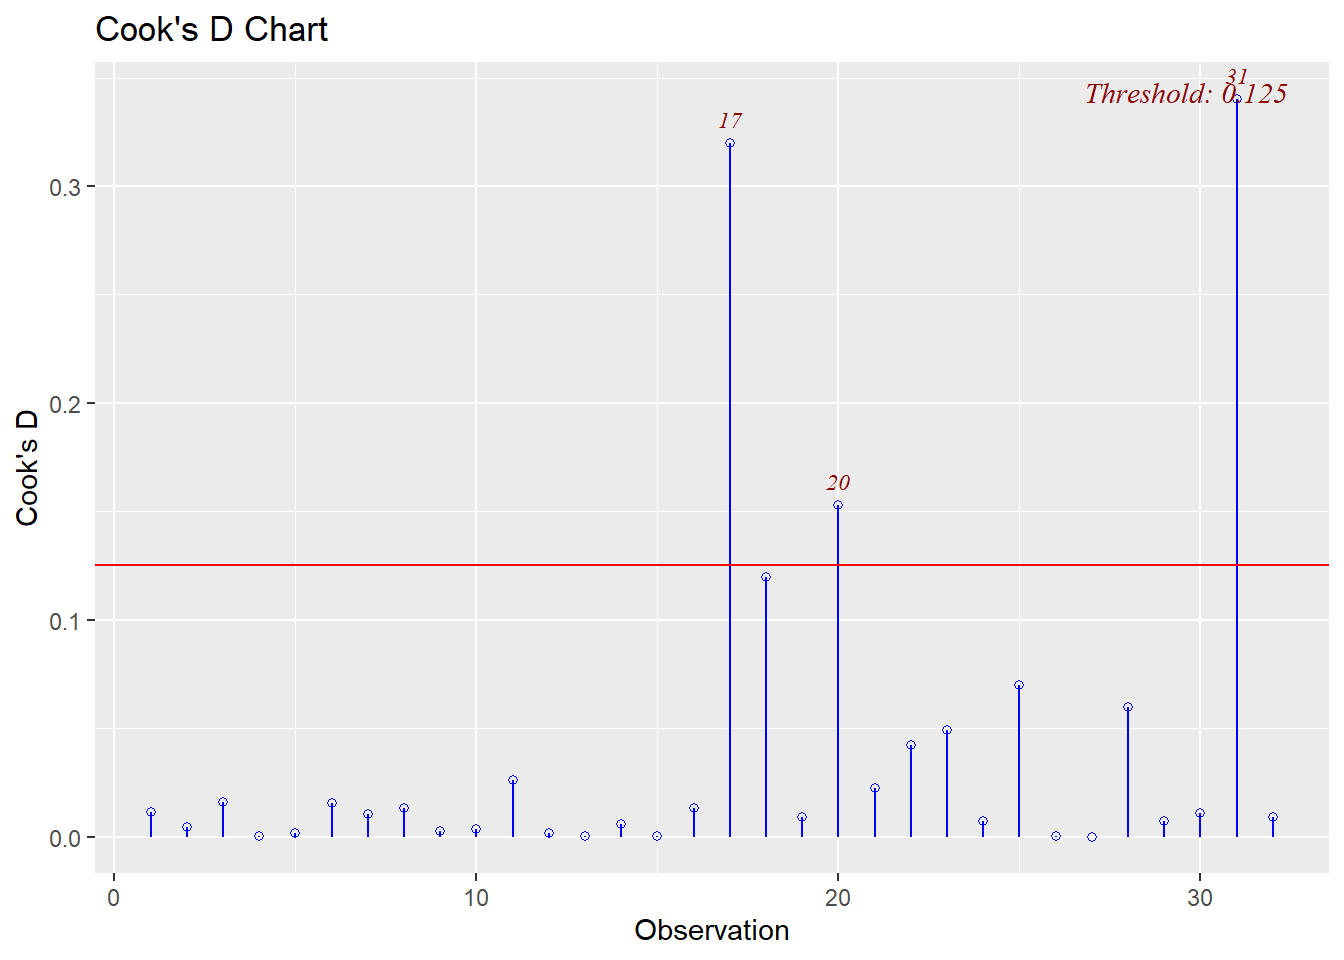
\includegraphics{quick-r-statistics_files/figure-latex/unnamed-chunk-121-2.pdf}

看residual和leverage。

\begin{Shaded}
\begin{Highlighting}[]
\FunctionTok{library}\NormalTok{(olsrr)}
\FunctionTok{ols\_plot\_resid\_lev}\NormalTok{(model.mpg.whd)}
\end{Highlighting}
\end{Shaded}

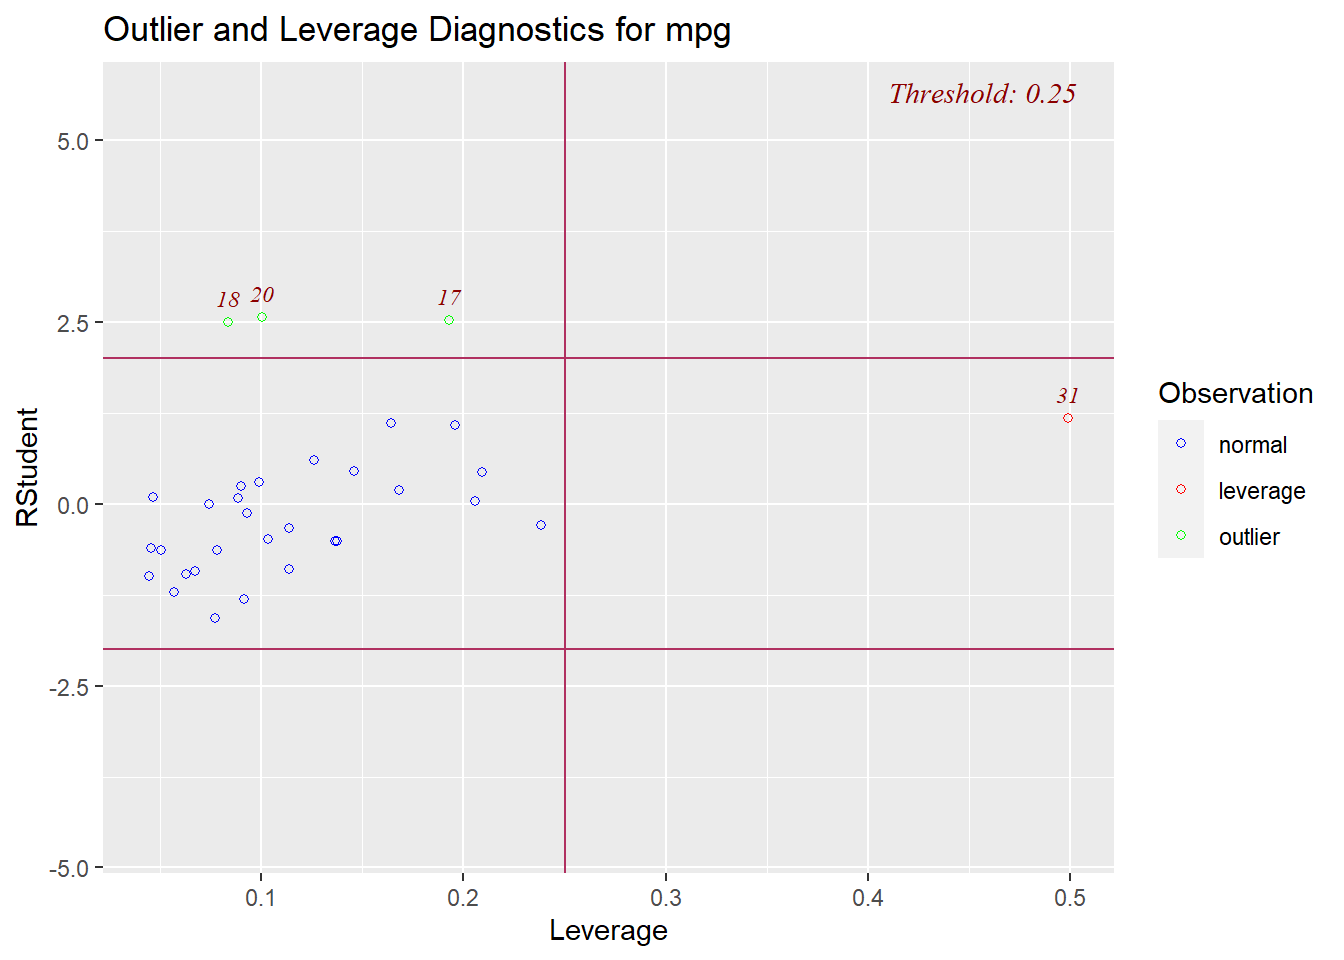
\includegraphics{quick-r-statistics_files/figure-latex/unnamed-chunk-122-1.pdf}

\hypertarget{homoscedasticityux8a3aux65b7}{%
\subsection{Homoscedasticity診斷}\label{homoscedasticityux8a3aux65b7}}

看residual和fit。

\begin{Shaded}
\begin{Highlighting}[]
\FunctionTok{ols\_plot\_resid\_stud\_fit}\NormalTok{(model.mpg.whd)}
\end{Highlighting}
\end{Shaded}

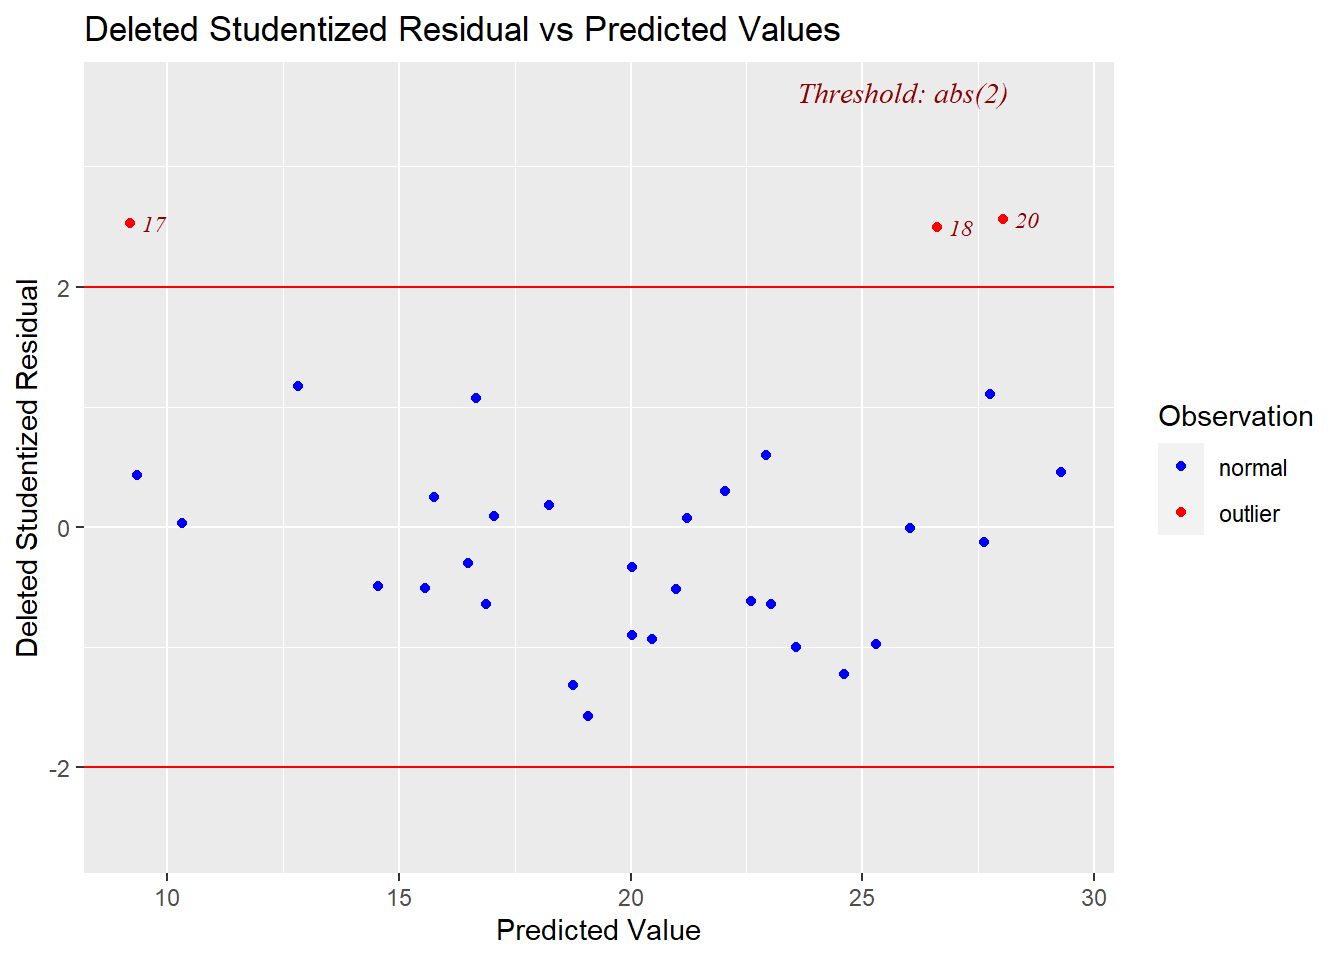
\includegraphics{quick-r-statistics_files/figure-latex/unnamed-chunk-123-1.pdf}

\hypertarget{ux5171ux7ddaux6027multicollinearityux7684ux6aa2ux9a57}{%
\subsection{共線性multicollinearity的檢驗}\label{ux5171ux7ddaux6027multicollinearityux7684ux6aa2ux9a57}}

看vif和tolerance。最大的VIF大於10要注意、平均的VIF大於1可能有偏誤;tolerance小於0.1要注意、tolerance小於0.2可能有問題。

\begin{Shaded}
\begin{Highlighting}[]
\FunctionTok{library}\NormalTok{(car)}
\FunctionTok{vif}\NormalTok{(model.mpg.whd)}
\end{Highlighting}
\end{Shaded}

\begin{verbatim}
##       wt       hp     disp 
## 4.844618 2.736633 7.324517
\end{verbatim}

\begin{Shaded}
\begin{Highlighting}[]
\DecValTok{1}\SpecialCharTok{/}\FunctionTok{vif}\NormalTok{(model.mpg.whd)}
\end{Highlighting}
\end{Shaded}

\begin{verbatim}
##        wt        hp      disp 
## 0.2064146 0.3654126 0.1365278
\end{verbatim}

\hypertarget{ux8aa4ux5deeux5e38ux614bux7684ux6aa2ux5b9a}{%
\subsection{誤差常態的檢定}\label{ux8aa4ux5deeux5e38ux614bux7684ux6aa2ux5b9a}}

residuals常態分配的檢定。

\begin{Shaded}
\begin{Highlighting}[]
\FunctionTok{shapiro.test}\NormalTok{(}\FunctionTok{residuals}\NormalTok{(model.mpg.whd))}
\end{Highlighting}
\end{Shaded}

\begin{verbatim}
## 
##  Shapiro-Wilk normality test
## 
## data:  residuals(model.mpg.whd)
## W = 0.92734, p-value = 0.03305
\end{verbatim}

\hypertarget{ux81eaux76f8ux95dcux6aa2ux9a57}{%
\subsection{自相關檢驗}\label{ux81eaux76f8ux95dcux6aa2ux9a57}}

用Durbin-Watson test看是否有autocorrelation。

\begin{Shaded}
\begin{Highlighting}[]
\FunctionTok{library}\NormalTok{(car)}
\FunctionTok{dwt}\NormalTok{(model.mpg.whd)}
\end{Highlighting}
\end{Shaded}

\begin{verbatim}
##  lag Autocorrelation D-W Statistic p-value
##    1       0.2926117      1.367284    0.03
##  Alternative hypothesis: rho != 0
\end{verbatim}

\begin{Shaded}
\begin{Highlighting}[]
\FunctionTok{durbinWatsonTest}\NormalTok{(model.mpg.whd)}
\end{Highlighting}
\end{Shaded}

\begin{verbatim}
##  lag Autocorrelation D-W Statistic p-value
##    1       0.2926117      1.367284    0.04
##  Alternative hypothesis: rho != 0
\end{verbatim}

\hypertarget{ux7d9cux5408ux6aa2ux9a57}{%
\subsection{綜合檢驗}\label{ux7d9cux5408ux6aa2ux9a57}}

可用內建的plot()功能一次看上述檢驗。若加which=1:6可看更多。

\begin{Shaded}
\begin{Highlighting}[]
\FunctionTok{plot}\NormalTok{(model.mpg.whd)}
\end{Highlighting}
\end{Shaded}

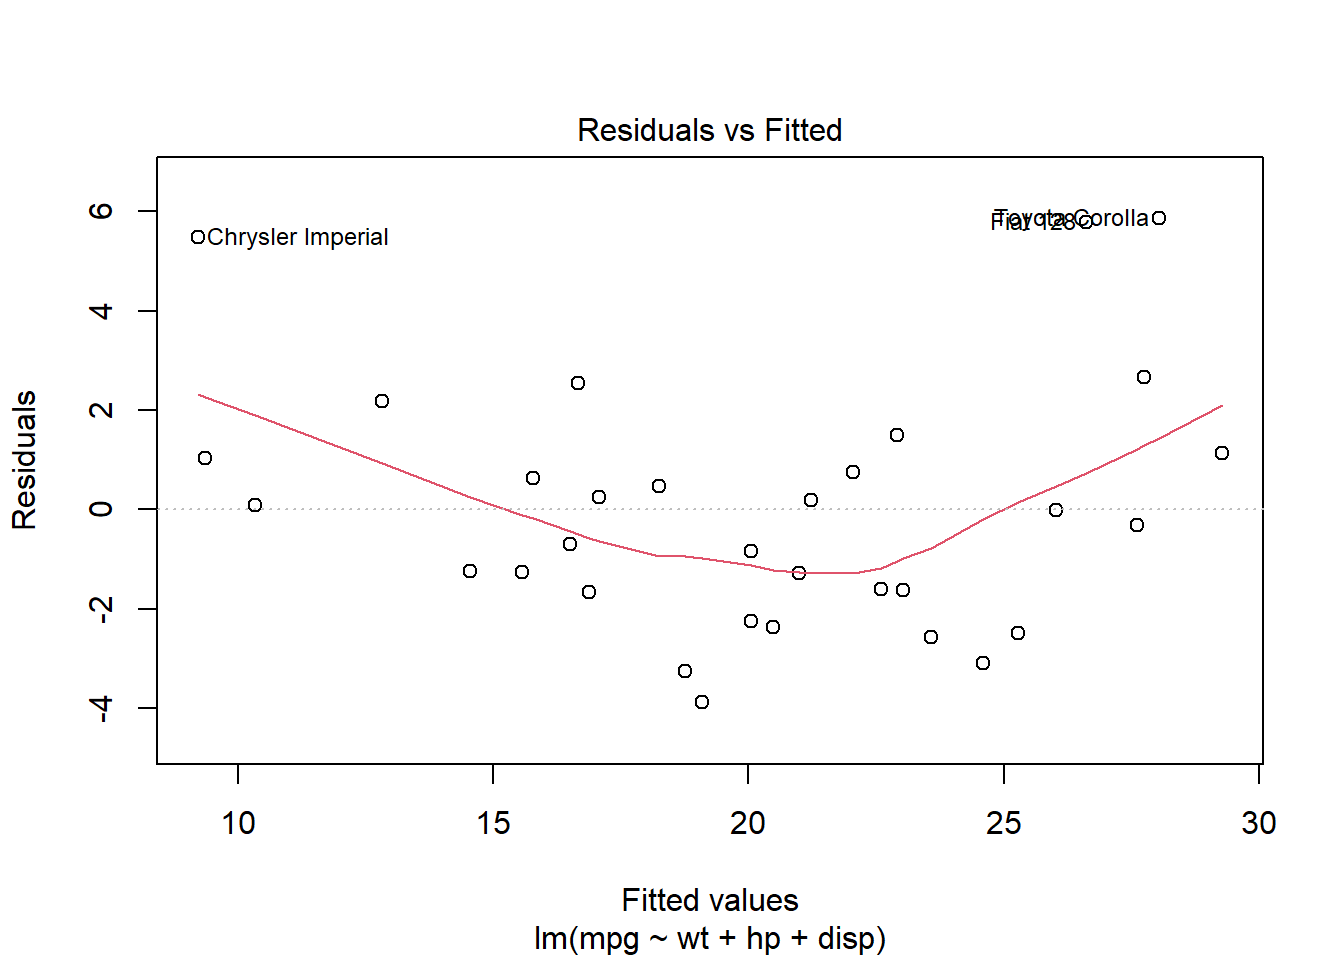
\includegraphics{quick-r-statistics_files/figure-latex/unnamed-chunk-127-1.pdf} 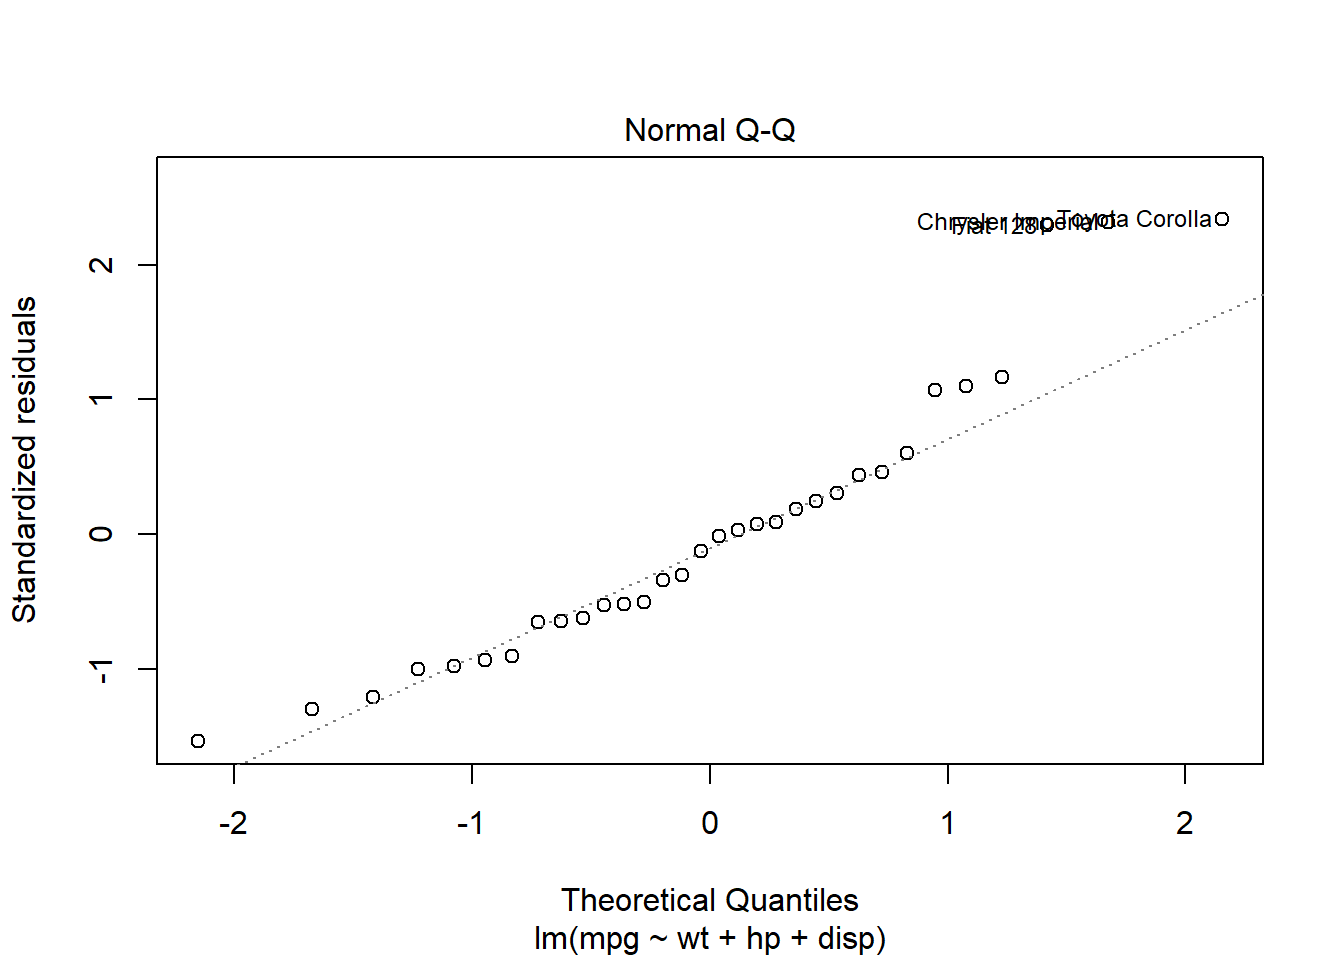
\includegraphics{quick-r-statistics_files/figure-latex/unnamed-chunk-127-2.pdf} 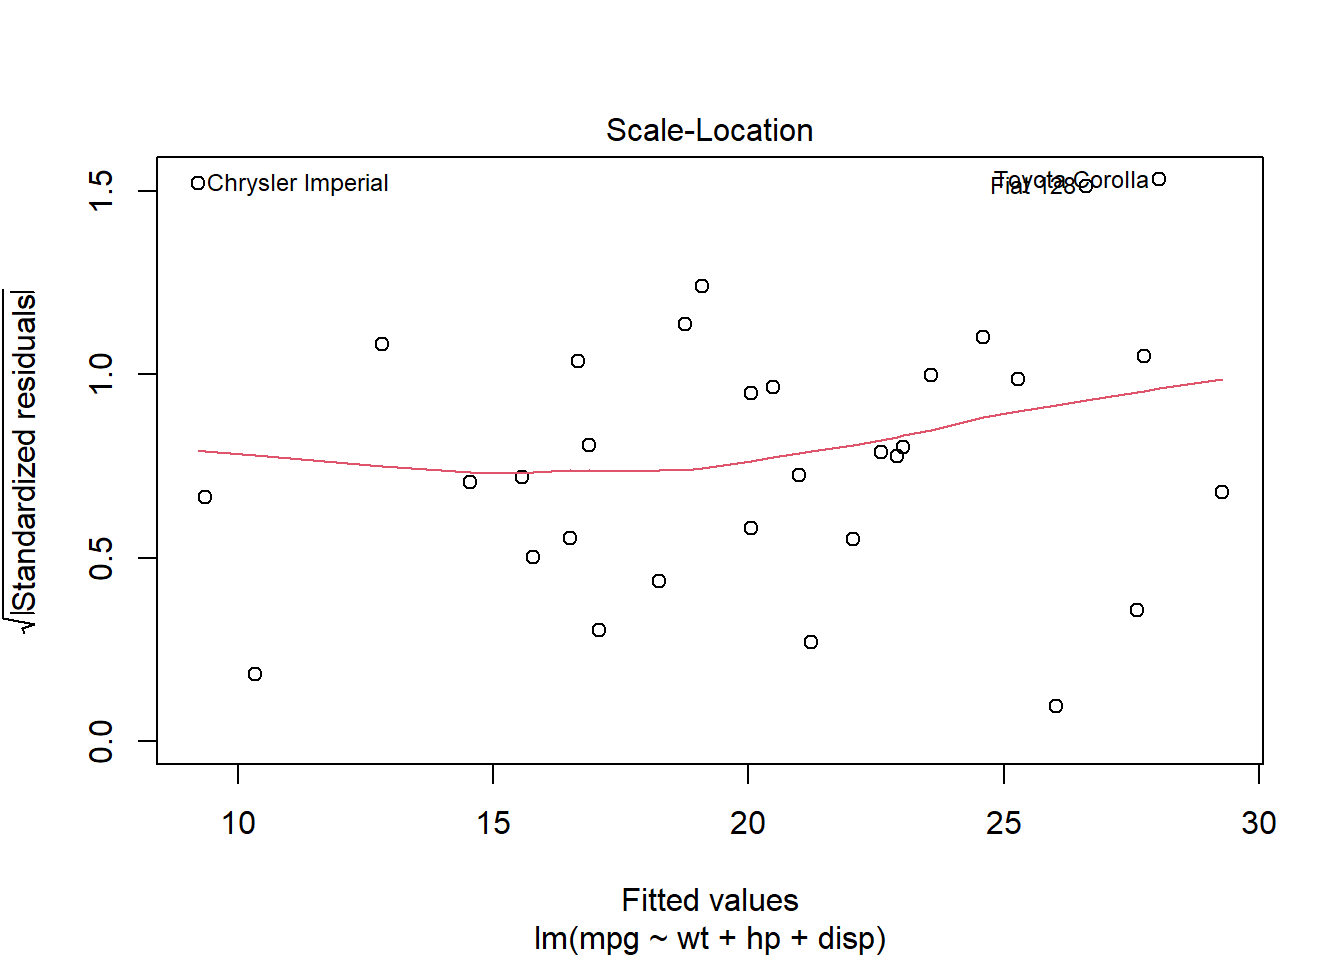
\includegraphics{quick-r-statistics_files/figure-latex/unnamed-chunk-127-3.pdf} 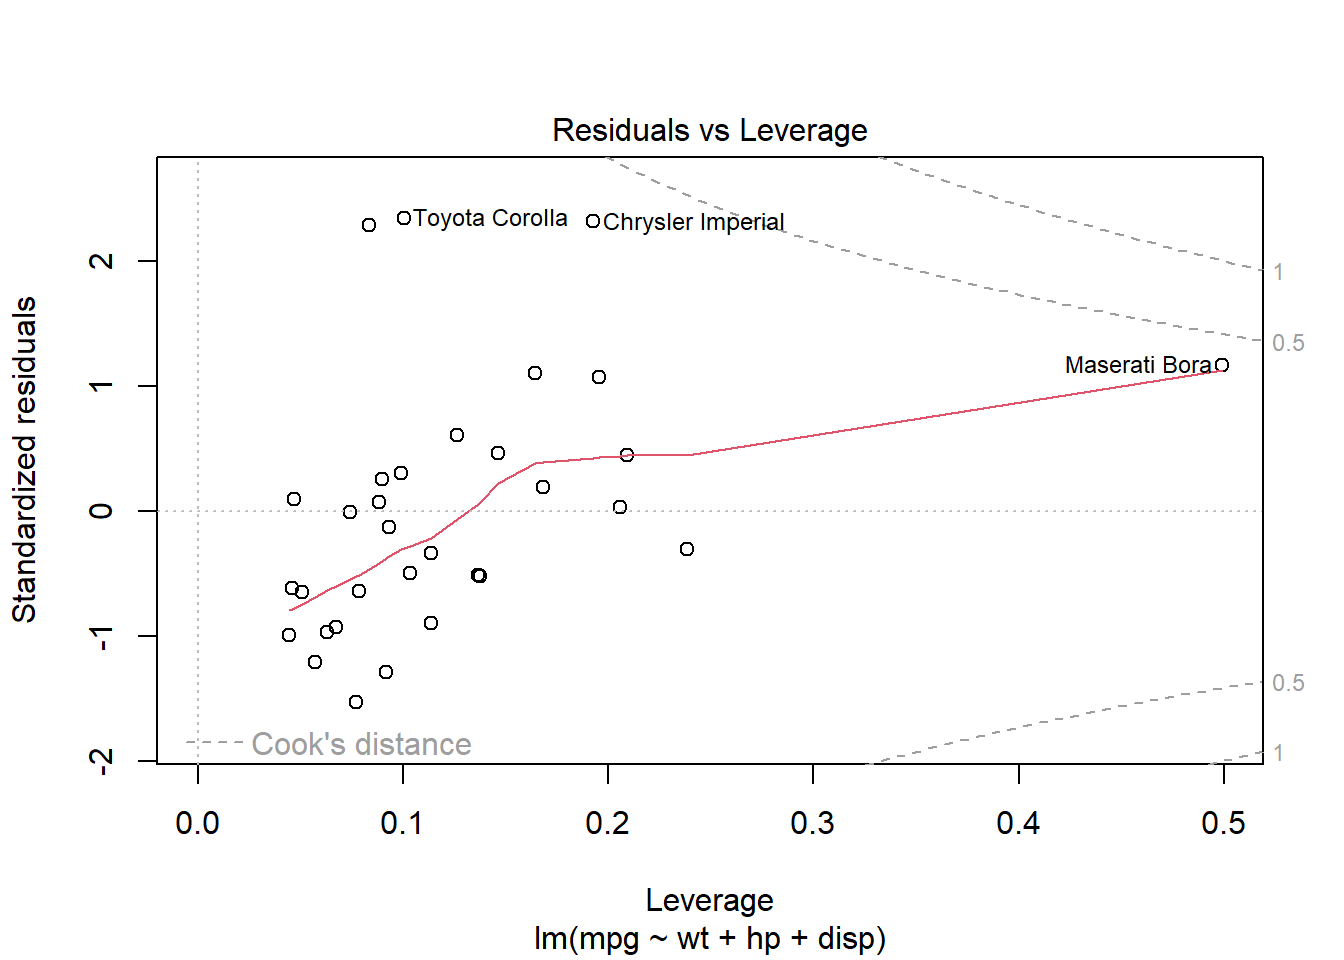
\includegraphics{quick-r-statistics_files/figure-latex/unnamed-chunk-127-4.pdf}

也可以將圖表放在一起看。

\begin{Shaded}
\begin{Highlighting}[]
\FunctionTok{par}\NormalTok{(}\AttributeTok{mfrow=}\FunctionTok{c}\NormalTok{(}\DecValTok{2}\NormalTok{,}\DecValTok{2}\NormalTok{))}
\FunctionTok{plot}\NormalTok{(model.mpg.whd)}
\end{Highlighting}
\end{Shaded}

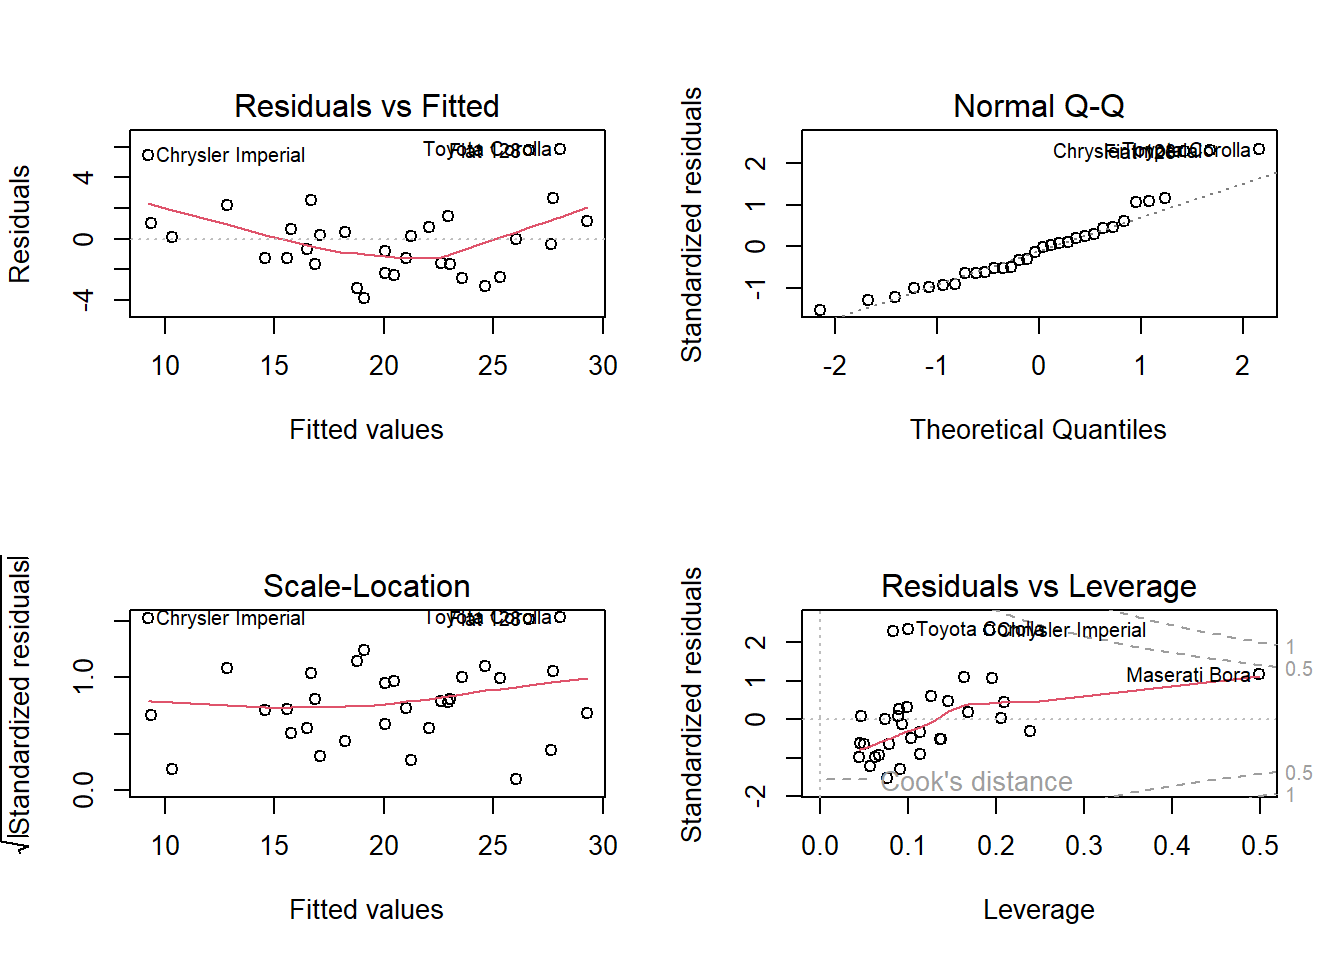
\includegraphics{quick-r-statistics_files/figure-latex/unnamed-chunk-128-1.pdf}

\begin{Shaded}
\begin{Highlighting}[]
\FunctionTok{par}\NormalTok{(}\AttributeTok{mfrow=}\FunctionTok{c}\NormalTok{(}\DecValTok{1}\NormalTok{,}\DecValTok{1}\NormalTok{))}
\end{Highlighting}
\end{Shaded}

或以performance這個package來看迴歸的假設。

\begin{Shaded}
\begin{Highlighting}[]
\FunctionTok{library}\NormalTok{(performance)}
\FunctionTok{library}\NormalTok{(see)}
\FunctionTok{library}\NormalTok{(patchwork)}
\FunctionTok{check\_model}\NormalTok{(model.mpg.whd)}
\end{Highlighting}
\end{Shaded}

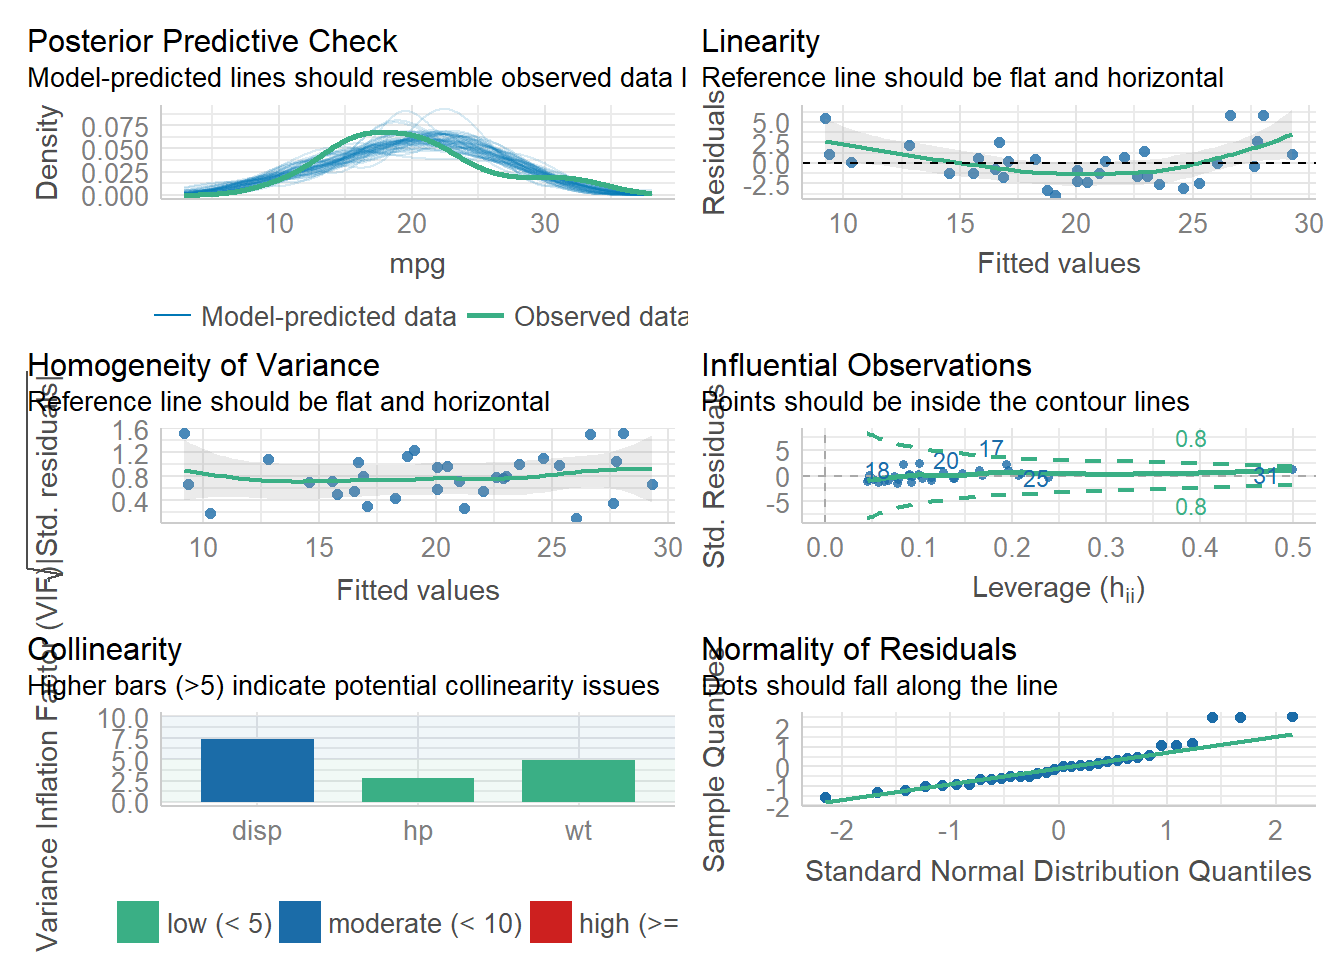
\includegraphics{quick-r-statistics_files/figure-latex/unnamed-chunk-129-1.pdf}

計算各統計量並儲存。

\begin{Shaded}
\begin{Highlighting}[]
\NormalTok{mtcars}\SpecialCharTok{$}\NormalTok{residuals }\OtherTok{\textless{}{-}} \FunctionTok{resid}\NormalTok{(model.mpg.whd)  }
\NormalTok{mtcars}\SpecialCharTok{$}\NormalTok{standardized.residuals }\OtherTok{\textless{}{-}} \FunctionTok{rstandard}\NormalTok{(model.mpg.whd)}
\NormalTok{mtcars}\SpecialCharTok{$}\NormalTok{studentized.residuals }\OtherTok{\textless{}{-}} \FunctionTok{rstudent}\NormalTok{(model.mpg.whd)}
\NormalTok{mtcars}\SpecialCharTok{$}\NormalTok{cooks.distance }\OtherTok{\textless{}{-}} \FunctionTok{cooks.distance}\NormalTok{(model.mpg.whd)}
\NormalTok{mtcars}\SpecialCharTok{$}\NormalTok{leverage }\OtherTok{\textless{}{-}} \FunctionTok{hatvalues}\NormalTok{(model.mpg.whd)}
\NormalTok{mtcars }\OtherTok{\textless{}{-}} \FunctionTok{cbind}\NormalTok{(mtcars, }\FunctionTok{dfbetas}\NormalTok{(model.mpg.whd))}
\FunctionTok{names}\NormalTok{(mtcars)[}\DecValTok{12}\SpecialCharTok{:}\DecValTok{15}\NormalTok{] }\OtherTok{\textless{}{-}} \FunctionTok{c}\NormalTok{(}\StringTok{\textquotesingle{}db\_intercept\textquotesingle{}}\NormalTok{, }\StringTok{\textquotesingle{}db\_wt\textquotesingle{}}\NormalTok{, }\StringTok{\textquotesingle{}db\_hp\textquotesingle{}}\NormalTok{, }\StringTok{\textquotesingle{}db\_disp\textquotesingle{}}\NormalTok{)}
\NormalTok{mtcars}\SpecialCharTok{$}\NormalTok{dffit }\OtherTok{\textless{}{-}} \FunctionTok{dffits}\NormalTok{(model.mpg.whd)}
\NormalTok{mtcars}\SpecialCharTok{$}\NormalTok{fitted }\OtherTok{\textless{}{-}} \FunctionTok{fitted}\NormalTok{(model.mpg.whd)}
\end{Highlighting}
\end{Shaded}

\hypertarget{ux9010ux6b65ux8ff4ux6b78}{%
\section{逐步迴歸}\label{ux9010ux6b65ux8ff4ux6b78}}

\hypertarget{ux524dux5411ux6cd5}{%
\subsection{前向法}\label{ux524dux5411ux6cd5}}

用lm()做逐步回歸。以下為前向法。

\begin{Shaded}
\begin{Highlighting}[]
\NormalTok{mtcars2 }\OtherTok{\textless{}{-}}\NormalTok{ mtcars[}\FunctionTok{c}\NormalTok{(}\DecValTok{1}\NormalTok{,}\DecValTok{6}\NormalTok{,}\DecValTok{4}\NormalTok{,}\DecValTok{3}\NormalTok{)]}
\NormalTok{nullM }\OtherTok{\textless{}{-}} \FunctionTok{lm}\NormalTok{(mpg }\SpecialCharTok{\textasciitilde{}} \DecValTok{1}\NormalTok{, }\AttributeTok{data =}\NormalTok{ mtcars2)}
\NormalTok{fullM }\OtherTok{\textless{}{-}} \FunctionTok{lm}\NormalTok{(mpg }\SpecialCharTok{\textasciitilde{}}\NormalTok{ ., }\AttributeTok{data =}\NormalTok{ mtcars2)}
\NormalTok{forM }\OtherTok{\textless{}{-}} \FunctionTok{step}\NormalTok{(nullM, }\AttributeTok{scope=}\FunctionTok{list}\NormalTok{(}\AttributeTok{lower=}\NormalTok{nullM, }\AttributeTok{upper=}\NormalTok{fullM), }\AttributeTok{direction=}\StringTok{"forward"}\NormalTok{)}
\end{Highlighting}
\end{Shaded}

\begin{verbatim}
## Start:  AIC=115.94
## mpg ~ 1
## 
##        Df Sum of Sq     RSS     AIC
## + wt    1    847.73  278.32  73.217
## + disp  1    808.89  317.16  77.397
## + hp    1    678.37  447.67  88.427
## <none>              1126.05 115.943
## 
## Step:  AIC=73.22
## mpg ~ wt
## 
##        Df Sum of Sq    RSS    AIC
## + hp    1    83.274 195.05 63.840
## + disp  1    31.639 246.68 71.356
## <none>              278.32 73.217
## 
## Step:  AIC=63.84
## mpg ~ wt + hp
## 
##        Df Sum of Sq    RSS    AIC
## <none>              195.05 63.840
## + disp  1   0.05708 194.99 65.831
\end{verbatim}

\begin{Shaded}
\begin{Highlighting}[]
\FunctionTok{summary}\NormalTok{(forM)}
\end{Highlighting}
\end{Shaded}

\begin{verbatim}
## 
## Call:
## lm(formula = mpg ~ wt + hp, data = mtcars2)
## 
## Residuals:
##    Min     1Q Median     3Q    Max 
## -3.941 -1.600 -0.182  1.050  5.854 
## 
## Coefficients:
##             Estimate Std. Error t value Pr(>|t|)    
## (Intercept) 37.22727    1.59879  23.285  < 2e-16 ***
## wt          -3.87783    0.63273  -6.129 1.12e-06 ***
## hp          -0.03177    0.00903  -3.519  0.00145 ** 
## ---
## Signif. codes:  0 '***' 0.001 '**' 0.01 '*' 0.05 '.' 0.1 ' ' 1
## 
## Residual standard error: 2.593 on 29 degrees of freedom
## Multiple R-squared:  0.8268, Adjusted R-squared:  0.8148 
## F-statistic: 69.21 on 2 and 29 DF,  p-value: 9.109e-12
\end{verbatim}

\hypertarget{ux5f8cux5411ux6cd5}{%
\subsection{後向法}\label{ux5f8cux5411ux6cd5}}

backward method。

\begin{Shaded}
\begin{Highlighting}[]
\NormalTok{fullM }\OtherTok{\textless{}{-}} \FunctionTok{lm}\NormalTok{(mpg }\SpecialCharTok{\textasciitilde{}}\NormalTok{ ., }\AttributeTok{data =}\NormalTok{ mtcars2)}
\CommentTok{\# backM \textless{}{-} step(fullM, scope=list(upper=fullM), direction=\textquotesingle{}backward\textquotesingle{}) \# 完整寫法}
\NormalTok{backM }\OtherTok{\textless{}{-}} \FunctionTok{step}\NormalTok{(fullM, }\AttributeTok{direction=}\StringTok{\textquotesingle{}backward\textquotesingle{}}\NormalTok{) }
\end{Highlighting}
\end{Shaded}

\begin{verbatim}
## Start:  AIC=65.83
## mpg ~ wt + hp + disp
## 
##        Df Sum of Sq    RSS    AIC
## - disp  1     0.057 195.05 63.840
## <none>              194.99 65.831
## - hp    1    51.692 246.68 71.356
## - wt    1    88.503 283.49 75.806
## 
## Step:  AIC=63.84
## mpg ~ wt + hp
## 
##        Df Sum of Sq    RSS    AIC
## <none>              195.05 63.840
## - hp    1    83.274 278.32 73.217
## - wt    1   252.627 447.67 88.427
\end{verbatim}

\begin{Shaded}
\begin{Highlighting}[]
\FunctionTok{summary}\NormalTok{(backM)}
\end{Highlighting}
\end{Shaded}

\begin{verbatim}
## 
## Call:
## lm(formula = mpg ~ wt + hp, data = mtcars2)
## 
## Residuals:
##    Min     1Q Median     3Q    Max 
## -3.941 -1.600 -0.182  1.050  5.854 
## 
## Coefficients:
##             Estimate Std. Error t value Pr(>|t|)    
## (Intercept) 37.22727    1.59879  23.285  < 2e-16 ***
## wt          -3.87783    0.63273  -6.129 1.12e-06 ***
## hp          -0.03177    0.00903  -3.519  0.00145 ** 
## ---
## Signif. codes:  0 '***' 0.001 '**' 0.01 '*' 0.05 '.' 0.1 ' ' 1
## 
## Residual standard error: 2.593 on 29 degrees of freedom
## Multiple R-squared:  0.8268, Adjusted R-squared:  0.8148 
## F-statistic: 69.21 on 2 and 29 DF,  p-value: 9.109e-12
\end{verbatim}

\hypertarget{ux9010ux6b65ux6cd5}{%
\subsection{逐步法}\label{ux9010ux6b65ux6cd5}}

Stepwise method。

\hypertarget{ux5f9efull-modelux958bux59cb}{%
\subsubsection{從full model開始}\label{ux5f9efull-modelux958bux59cb}}

\begin{Shaded}
\begin{Highlighting}[]
\NormalTok{fullM }\OtherTok{\textless{}{-}} \FunctionTok{lm}\NormalTok{(mpg }\SpecialCharTok{\textasciitilde{}}\NormalTok{ ., }\AttributeTok{data =}\NormalTok{ mtcars2)}
\CommentTok{\# stepM1 \textless{}{-} step(fullM, scope = list(upper=fullM), direction="both") \# 完整寫法}
\NormalTok{stepM1 }\OtherTok{\textless{}{-}} \FunctionTok{step}\NormalTok{(fullM, }\AttributeTok{direction=}\StringTok{"both"}\NormalTok{) }
\end{Highlighting}
\end{Shaded}

\begin{verbatim}
## Start:  AIC=65.83
## mpg ~ wt + hp + disp
## 
##        Df Sum of Sq    RSS    AIC
## - disp  1     0.057 195.05 63.840
## <none>              194.99 65.831
## - hp    1    51.692 246.68 71.356
## - wt    1    88.503 283.49 75.806
## 
## Step:  AIC=63.84
## mpg ~ wt + hp
## 
##        Df Sum of Sq    RSS    AIC
## <none>              195.05 63.840
## + disp  1     0.057 194.99 65.831
## - hp    1    83.274 278.32 73.217
## - wt    1   252.627 447.67 88.427
\end{verbatim}

\hypertarget{ux5f9enull-modelux958bux59cb}{%
\subsubsection{從null model開始}\label{ux5f9enull-modelux958bux59cb}}

結果可能會與從full model開始不同。

\begin{Shaded}
\begin{Highlighting}[]
\NormalTok{nullM }\OtherTok{\textless{}{-}} \FunctionTok{lm}\NormalTok{(mpg }\SpecialCharTok{\textasciitilde{}} \DecValTok{1}\NormalTok{, }\AttributeTok{data =}\NormalTok{ mtcars2)}
\NormalTok{stepM2 }\OtherTok{\textless{}{-}} \FunctionTok{step}\NormalTok{(nullM, }\AttributeTok{scope =} \FunctionTok{list}\NormalTok{(}\AttributeTok{upper=}\NormalTok{fullM), }\AttributeTok{direction=}\StringTok{"both"}\NormalTok{)}
\end{Highlighting}
\end{Shaded}

\begin{verbatim}
## Start:  AIC=115.94
## mpg ~ 1
## 
##        Df Sum of Sq     RSS     AIC
## + wt    1    847.73  278.32  73.217
## + disp  1    808.89  317.16  77.397
## + hp    1    678.37  447.67  88.427
## <none>              1126.05 115.943
## 
## Step:  AIC=73.22
## mpg ~ wt
## 
##        Df Sum of Sq     RSS     AIC
## + hp    1     83.27  195.05  63.840
## + disp  1     31.64  246.68  71.356
## <none>               278.32  73.217
## - wt    1    847.73 1126.05 115.943
## 
## Step:  AIC=63.84
## mpg ~ wt + hp
## 
##        Df Sum of Sq    RSS    AIC
## <none>              195.05 63.840
## + disp  1     0.057 194.99 65.831
## - hp    1    83.274 278.32 73.217
## - wt    1   252.627 447.67 88.427
\end{verbatim}

\begin{Shaded}
\begin{Highlighting}[]
\FunctionTok{summary}\NormalTok{(stepM1)}
\end{Highlighting}
\end{Shaded}

\begin{verbatim}
## 
## Call:
## lm(formula = mpg ~ wt + hp, data = mtcars2)
## 
## Residuals:
##    Min     1Q Median     3Q    Max 
## -3.941 -1.600 -0.182  1.050  5.854 
## 
## Coefficients:
##             Estimate Std. Error t value Pr(>|t|)    
## (Intercept) 37.22727    1.59879  23.285  < 2e-16 ***
## wt          -3.87783    0.63273  -6.129 1.12e-06 ***
## hp          -0.03177    0.00903  -3.519  0.00145 ** 
## ---
## Signif. codes:  0 '***' 0.001 '**' 0.01 '*' 0.05 '.' 0.1 ' ' 1
## 
## Residual standard error: 2.593 on 29 degrees of freedom
## Multiple R-squared:  0.8268, Adjusted R-squared:  0.8148 
## F-statistic: 69.21 on 2 and 29 DF,  p-value: 9.109e-12
\end{verbatim}

\begin{Shaded}
\begin{Highlighting}[]
\FunctionTok{summary}\NormalTok{(stepM2)}
\end{Highlighting}
\end{Shaded}

\begin{verbatim}
## 
## Call:
## lm(formula = mpg ~ wt + hp, data = mtcars2)
## 
## Residuals:
##    Min     1Q Median     3Q    Max 
## -3.941 -1.600 -0.182  1.050  5.854 
## 
## Coefficients:
##             Estimate Std. Error t value Pr(>|t|)    
## (Intercept) 37.22727    1.59879  23.285  < 2e-16 ***
## wt          -3.87783    0.63273  -6.129 1.12e-06 ***
## hp          -0.03177    0.00903  -3.519  0.00145 ** 
## ---
## Signif. codes:  0 '***' 0.001 '**' 0.01 '*' 0.05 '.' 0.1 ' ' 1
## 
## Residual standard error: 2.593 on 29 degrees of freedom
## Multiple R-squared:  0.8268, Adjusted R-squared:  0.8148 
## F-statistic: 69.21 on 2 and 29 DF,  p-value: 9.109e-12
\end{verbatim}

\hypertarget{ux53e6ux4e00ux7a2eux4f5cux6cd5}{%
\subsubsection{另一種作法}\label{ux53e6ux4e00ux7a2eux4f5cux6cd5}}

可用stepAIC()來做逐步回歸。沒指定scope時會用backward;指定scope時會用both。可用direction來指定forward、backward或both。

\begin{Shaded}
\begin{Highlighting}[]
\FunctionTok{library}\NormalTok{(MASS)}
\FunctionTok{summary}\NormalTok{(}\FunctionTok{stepAIC}\NormalTok{(model.mpg.whd)) }\CommentTok{\#沒指定scope時會用backward}
\end{Highlighting}
\end{Shaded}

\begin{verbatim}
## Start:  AIC=65.83
## mpg ~ wt + hp + disp
## 
##        Df Sum of Sq    RSS    AIC
## - disp  1     0.057 195.05 63.840
## <none>              194.99 65.831
## - hp    1    51.692 246.68 71.356
## - wt    1    88.503 283.49 75.806
## 
## Step:  AIC=63.84
## mpg ~ wt + hp
## 
##        Df Sum of Sq    RSS    AIC
## <none>              195.05 63.840
## - hp    1    83.274 278.32 73.217
## - wt    1   252.627 447.67 88.427
\end{verbatim}

\begin{verbatim}
## 
## Call:
## lm(formula = mpg ~ wt + hp, data = mtcars)
## 
## Residuals:
##    Min     1Q Median     3Q    Max 
## -3.941 -1.600 -0.182  1.050  5.854 
## 
## Coefficients:
##             Estimate Std. Error t value Pr(>|t|)    
## (Intercept) 37.22727    1.59879  23.285  < 2e-16 ***
## wt          -3.87783    0.63273  -6.129 1.12e-06 ***
## hp          -0.03177    0.00903  -3.519  0.00145 ** 
## ---
## Signif. codes:  0 '***' 0.001 '**' 0.01 '*' 0.05 '.' 0.1 ' ' 1
## 
## Residual standard error: 2.593 on 29 degrees of freedom
## Multiple R-squared:  0.8268, Adjusted R-squared:  0.8148 
## F-statistic: 69.21 on 2 and 29 DF,  p-value: 9.109e-12
\end{verbatim}

\begin{Shaded}
\begin{Highlighting}[]
\FunctionTok{summary}\NormalTok{(}\FunctionTok{stepAIC}\NormalTok{(model.mpg.whd, }\AttributeTok{scope =} \FunctionTok{list}\NormalTok{(}\AttributeTok{upper =} \SpecialCharTok{\textasciitilde{}}\NormalTok{wt}\SpecialCharTok{+}\NormalTok{hp}\SpecialCharTok{+}\NormalTok{disp, }\AttributeTok{lower =} \SpecialCharTok{\textasciitilde{}}\DecValTok{1}\NormalTok{)))  }\CommentTok{\#指定scope時會用both}
\end{Highlighting}
\end{Shaded}

\begin{verbatim}
## Start:  AIC=65.83
## mpg ~ wt + hp + disp
## 
##        Df Sum of Sq    RSS    AIC
## - disp  1     0.057 195.05 63.840
## <none>              194.99 65.831
## - hp    1    51.692 246.68 71.356
## - wt    1    88.503 283.49 75.806
## 
## Step:  AIC=63.84
## mpg ~ wt + hp
## 
##        Df Sum of Sq    RSS    AIC
## <none>              195.05 63.840
## + disp  1     0.057 194.99 65.831
## - hp    1    83.274 278.32 73.217
## - wt    1   252.627 447.67 88.427
\end{verbatim}

\begin{verbatim}
## 
## Call:
## lm(formula = mpg ~ wt + hp, data = mtcars)
## 
## Residuals:
##    Min     1Q Median     3Q    Max 
## -3.941 -1.600 -0.182  1.050  5.854 
## 
## Coefficients:
##             Estimate Std. Error t value Pr(>|t|)    
## (Intercept) 37.22727    1.59879  23.285  < 2e-16 ***
## wt          -3.87783    0.63273  -6.129 1.12e-06 ***
## hp          -0.03177    0.00903  -3.519  0.00145 ** 
## ---
## Signif. codes:  0 '***' 0.001 '**' 0.01 '*' 0.05 '.' 0.1 ' ' 1
## 
## Residual standard error: 2.593 on 29 degrees of freedom
## Multiple R-squared:  0.8268, Adjusted R-squared:  0.8148 
## F-statistic: 69.21 on 2 and 29 DF,  p-value: 9.109e-12
\end{verbatim}

\hypertarget{ux985eux5225ux8b8aux9805ux7684ux8ff4ux6b78}{%
\section{類別變項的迴歸}\label{ux985eux5225ux8b8aux9805ux7684ux8ff4ux6b78}}

若只有兩個levels,可直接做迴歸。若有多個levels,可以dummy coding的方式來做。

\begin{Shaded}
\begin{Highlighting}[]
\NormalTok{mtcars}\SpecialCharTok{$}\NormalTok{cyl}\OtherTok{\textless{}{-}}\FunctionTok{factor}\NormalTok{(mtcars}\SpecialCharTok{$}\NormalTok{cyl)}
\FunctionTok{contrasts}\NormalTok{(mtcars}\SpecialCharTok{$}\NormalTok{cyl)}\OtherTok{\textless{}{-}}\FunctionTok{contr.treatment}\NormalTok{(}\DecValTok{3}\NormalTok{, }\AttributeTok{base =} \DecValTok{1}\NormalTok{) }\CommentTok{\#generate contrasts}
\NormalTok{mtcars}\SpecialCharTok{$}\NormalTok{cyl}
\end{Highlighting}
\end{Shaded}

\begin{verbatim}
##  [1] 6 6 4 6 8 6 8 4 4 6 6 8 8 8 8 8 8 4 4 4 4 8 8 8 8 4 4 4 8 6 8 4
## attr(,"contrasts")
##   2 3
## 4 0 0
## 6 1 0
## 8 0 1
## Levels: 4 6 8
\end{verbatim}

\begin{Shaded}
\begin{Highlighting}[]
\NormalTok{model.mpg.cyl }\OtherTok{\textless{}{-}} \FunctionTok{lm}\NormalTok{(mpg }\SpecialCharTok{\textasciitilde{}}\NormalTok{ cyl, }\AttributeTok{data =}\NormalTok{ mtcars)}
\FunctionTok{summary}\NormalTok{(model.mpg.cyl)}
\end{Highlighting}
\end{Shaded}

\begin{verbatim}
## 
## Call:
## lm(formula = mpg ~ cyl, data = mtcars)
## 
## Residuals:
##     Min      1Q  Median      3Q     Max 
## -5.2636 -1.8357  0.0286  1.3893  7.2364 
## 
## Coefficients:
##             Estimate Std. Error t value Pr(>|t|)    
## (Intercept)  26.6636     0.9718  27.437  < 2e-16 ***
## cyl2         -6.9208     1.5583  -4.441 0.000119 ***
## cyl3        -11.5636     1.2986  -8.905 8.57e-10 ***
## ---
## Signif. codes:  0 '***' 0.001 '**' 0.01 '*' 0.05 '.' 0.1 ' ' 1
## 
## Residual standard error: 3.223 on 29 degrees of freedom
## Multiple R-squared:  0.7325, Adjusted R-squared:  0.714 
## F-statistic:  39.7 on 2 and 29 DF,  p-value: 4.979e-09
\end{verbatim}

\hypertarget{moderation}{%
\chapter{調節效果分析}\label{moderation}}

本單元介紹如何以R語言做調節效果分析。

\hypertarget{ux8b80ux5165ux8cc7ux6599ux4e26ux756bux5716ux6aa2ux8996}{%
\section{讀入資料並畫圖檢視}\label{ux8b80ux5165ux8cc7ux6599ux4e26ux756bux5716ux6aa2ux8996}}

以JASP提供的\href{https://jasp-stats.org/wp-content/uploads/2020/03/moderation.csv}{moderation.csv}為例,以R做分析。

此資料測量觀察到的寵物鸚鵡與其主人的親近度(closeness)、主人表現出的情感行為量(affection)與鸚鵡的性別。

設定工作目錄。

讀入資料。

\begin{Shaded}
\begin{Highlighting}[]
\NormalTok{cData }\OtherTok{\textless{}{-}} \FunctionTok{read.table}\NormalTok{(}\StringTok{"moderation.csv"}\NormalTok{, }\AttributeTok{header=}\ConstantTok{TRUE}\NormalTok{, }\AttributeTok{sep=}\StringTok{","}\NormalTok{)}
\end{Highlighting}
\end{Shaded}

\begin{tabular}{r|r|r|l}
\hline
affection & closeness & gender\_dummy & gender\\
\hline
7 & 2 & 0 & Male\\
\hline
6 & 1 & 0 & Male\\
\hline
12 & 0 & 0 & Male\\
\hline
14 & 1 & 0 & Male\\
\hline
17 & 3 & 0 & Male\\
\hline
19 & 2 & 0 & Male\\
\hline
\end{tabular}

畫情感行為量與親近度的散佈圖,並依據不同的鸚鵡性別上色。

\begin{Shaded}
\begin{Highlighting}[]
\FunctionTok{library}\NormalTok{(ggplot2)}
\FunctionTok{qplot}\NormalTok{(affection, closeness, }\AttributeTok{colour =}\NormalTok{ gender, }\AttributeTok{data =}\NormalTok{ cData)}
\end{Highlighting}
\end{Shaded}

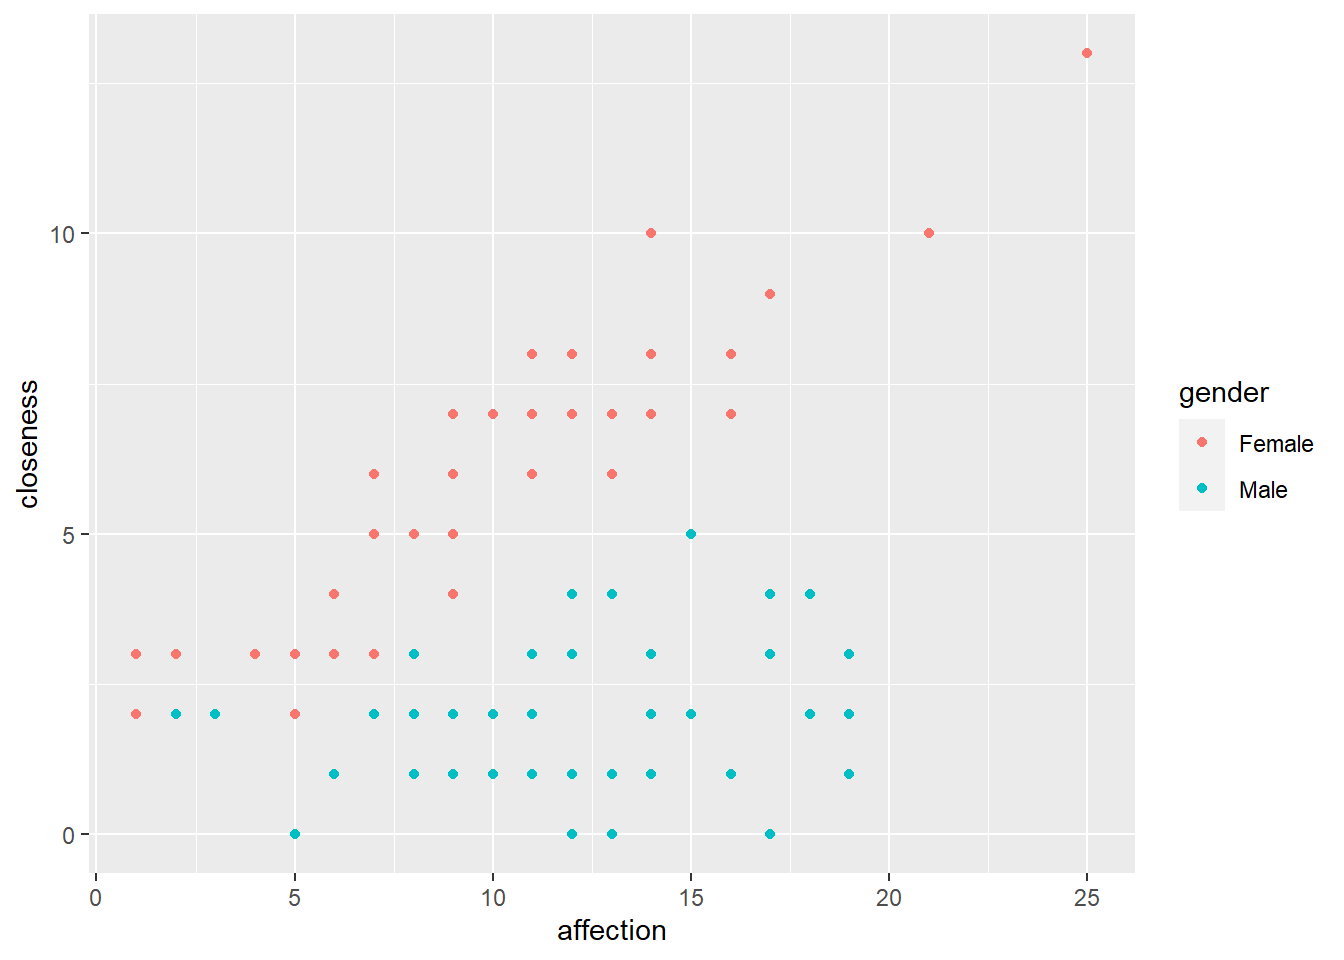
\includegraphics{quick-r-statistics_files/figure-latex/unnamed-chunk-143-1.pdf}

\hypertarget{ux8abfux7bc0ux8b8aux9805ux70baux985eux5225ux8b8aux9805}{%
\section{調節變項為類別變項}\label{ux8abfux7bc0ux8b8aux9805ux70baux985eux5225ux8b8aux9805}}

以下檢驗是否鸚鵡的性別可以調節主人表現出的情感對他們和鸚鵡之間的親密度。欲測試的想法為:主人表現出的情感對他們和鸚鵡之間的親密度有正向的效果;但對於雄性或雌性鸚鵡,這種效果可能會有所不同。意即,情感對親近的影響是由鸚鵡的性別調節的。

\hypertarget{ux6a21ux578bux6aa2ux9a57}{%
\subsection{模型檢驗}\label{ux6a21ux578bux6aa2ux9a57}}

將情感中心化後,以pequod套件中的lmres()函數做迴歸分析。此函數可直接以type=nested來看兩階段的迴歸模型,一為沒有交互作用項的,一為有交互作用項的,並檢驗加入交互作用項的模型是否顯著。

\begin{Shaded}
\begin{Highlighting}[]
\FunctionTok{library}\NormalTok{(pequod)}
\NormalTok{m1 }\OtherTok{\textless{}{-}} \FunctionTok{lmres}\NormalTok{(closeness}\SpecialCharTok{\textasciitilde{}}\NormalTok{affection}\SpecialCharTok{*}\NormalTok{gender, }\AttributeTok{centered=}\FunctionTok{c}\NormalTok{(}\StringTok{"affection"}\NormalTok{), }\AttributeTok{data=}\NormalTok{cData)}
\FunctionTok{summary}\NormalTok{(m1, }\AttributeTok{type=}\StringTok{"nested"}\NormalTok{)}
\end{Highlighting}
\end{Shaded}

\begin{verbatim}
## **Models**
## 
## Model 1: closeness ~ affection + genderMale
## <environment: 0x00000185d29df680>
## 
## Model 2: closeness ~ affection + genderMale + affection.XX.genderMale
## <environment: 0x00000185d29df680>
## 
## 
## **Statistics**
## 
##             R     R^2   Adj. R^2   Diff.R^2    F     df1  df2    p.value    
## Model 1    0.88   0.77      0.76       0.77 160.04   2.00   97 < 2.2e-16 ***
## Model 2:   0.93   0.86      0.86       0.09 197.52   3.00   96 < 2.2e-16 ***
## ---
## Signif. codes:  0 '***' 0.001 '**' 0.01 '*' 0.05 '.' 0.1 ' ' 1
## 
## 
## **F change**
## 
##   Res.Df RSS  Df Sum of Sq    F  Pr(>F)    
## 1     97 177                               
## 2     96 106   1        71 64.1 2.7e-12 ***
## ---
## Signif. codes:  0 '***' 0.001 '**' 0.01 '*' 0.05 '.' 0.1 ' ' 1
## 
## 
## **Coefficients**
## 
##                          Estimate    StdErr   t.value    beta   p.value    
## -- Model 1 --                                                              
##                                                                            
## (Intercept)               6.29135   0.19168  32.82144         < 2.2e-16 ***
## affection                 0.26269   0.02963   8.86462  0.4367 < 2.2e-16 ***
## genderMale               -4.46269   0.27189 -16.41354 -0.8085 < 2.2e-16 ***
##                                                                            
##                                                                            
## -- Model 2 --                                                              
##                                                                            
## (Intercept)               6.36873   0.14950  42.60126         < 2.2e-16 ***
## affection                 0.41746   0.03009  13.87403  0.6939 < 2.2e-16 ***
## genderMale               -4.42985   0.21165 -20.93042 -0.8026 < 2.2e-16 ***
## affection.XX.genderMale  -0.37521   0.04685  -8.00877 -0.3996 < 2.2e-16 ***
## ---
## Signif. codes:  0 '***' 0.001 '**' 0.01 '*' 0.05 '.' 0.1 ' ' 1
\end{verbatim}

由上面結果可知兩模型皆顯著,但加入交互作用的模型比未加入的模型可以多解釋9\%的變異量,此增加的解釋量達到顯著,\(\Delta\)R\^{}2 = .09, F(1,96) = 64.1, p \textless{} .001。迴歸式為closeness = 6.37 + 0.42 affection - 4.43 genderM - 0.38 affection\(\times\)genderM。

\hypertarget{simple-slopeux5206ux6790}{%
\subsection{Simple slope分析}\label{simple-slopeux5206ux6790}}

交互作用顯著,表示有調節效果。接著可做Simple slope分析,看鸚鵡的性別為雄性/雌性與情感在正/負一個標準差時的親密程度預測值。

\begin{Shaded}
\begin{Highlighting}[]
\NormalTok{Sim\_m1 }\OtherTok{\textless{}{-}} \FunctionTok{simpleSlope}\NormalTok{(m1, }\AttributeTok{pred=}\StringTok{"affection"}\NormalTok{, }\AttributeTok{mod1=}\StringTok{"genderMale"}\NormalTok{, }\AttributeTok{coded=}\StringTok{"genderMale"}\NormalTok{)}
\FunctionTok{summary}\NormalTok{(Sim\_m1)}
\end{Highlighting}
\end{Shaded}

\begin{verbatim}
## 
## ** Estimated points of closeness  **
## 
##                       Low affection (-1 SD) High affection (+1 SD)
## Low genderMale ( 0 )                 4.4440                 8.2935
## High genderMale ( 1 )                1.7441                 2.1337
## 
## 
## 
## ** Simple Slopes analysis ( df= 96 ) **
## 
##                       simple slope standard error t-value p.value    
## Low genderMale ( 0 )        0.4175         0.0301   13.87  <2e-16 ***
## High genderMale ( 1 )       0.0422         0.0359    1.18    0.24    
## ---
## Signif. codes:  0 '***' 0.001 '**' 0.01 '*' 0.05 '.' 0.1 ' ' 1
## 
## 
## 
## ** Bauer & Curran 95% CI **
## 
##            lower CI upper CI
## genderMale   0.9366   1.3778
\end{verbatim}

對上述Simple Slope作圖。

\begin{Shaded}
\begin{Highlighting}[]
\FunctionTok{PlotSlope}\NormalTok{(Sim\_m1)}
\end{Highlighting}
\end{Shaded}

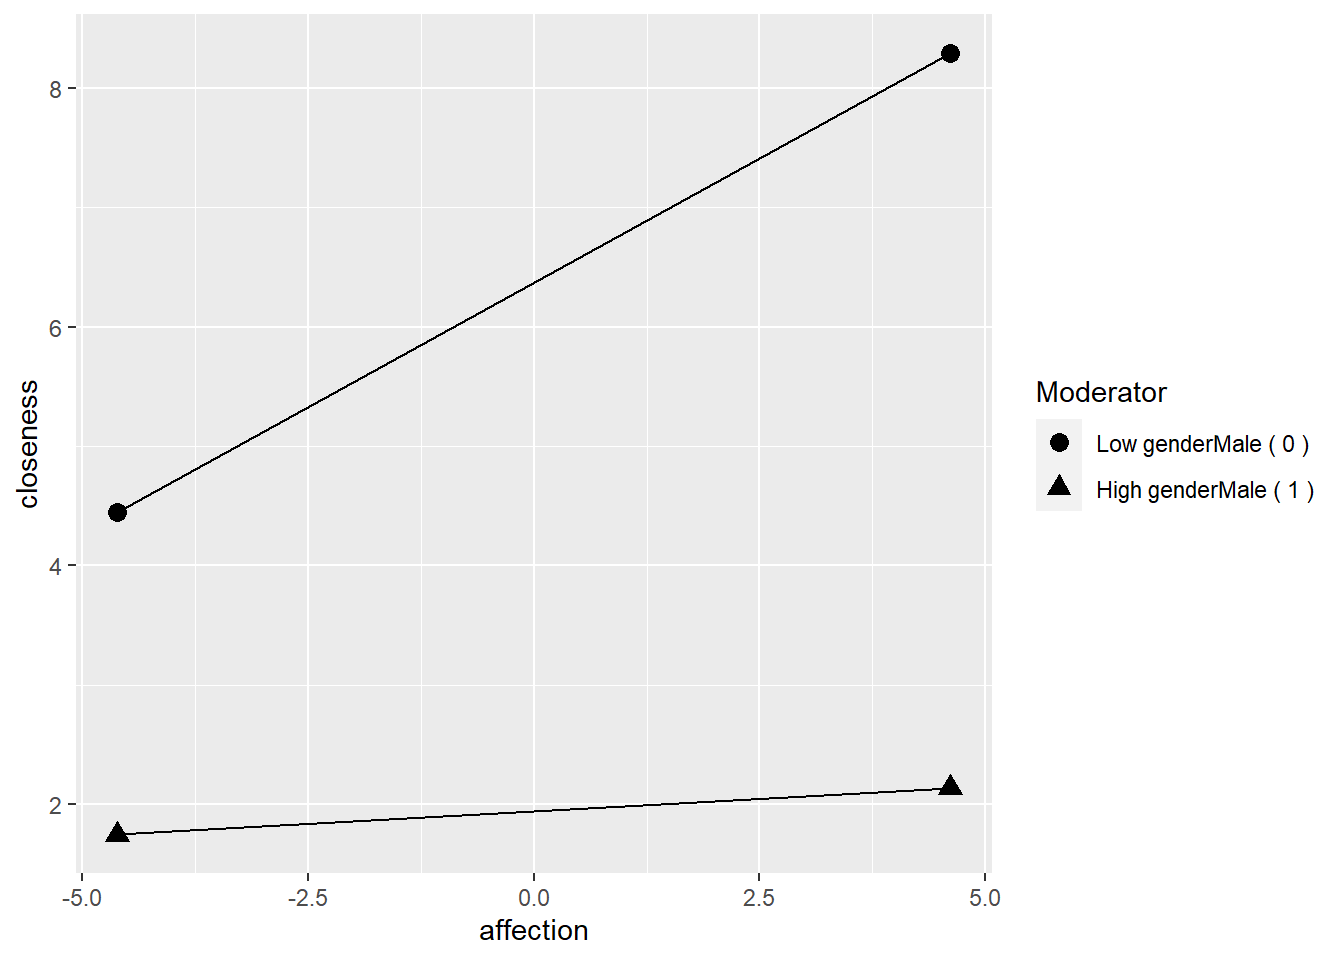
\includegraphics{quick-r-statistics_files/figure-latex/unnamed-chunk-146-1.pdf}

\hypertarget{ux8abfux7bc0ux8b8aux9805ux70baux9023ux7e8cux8b8aux9805}{%
\section{調節變項為連續變項}\label{ux8abfux7bc0ux8b8aux9805ux70baux9023ux7e8cux8b8aux9805}}

\hypertarget{ux6a21ux578bux6aa2ux9a57-1}{%
\subsection{模型檢驗}\label{ux6a21ux578bux6aa2ux9a57-1}}

資料與上面相同,但將情感作為調節變項、鸚鵡的性別做為預測項。迴歸式相同,故迴歸分析結果同上。

\begin{Shaded}
\begin{Highlighting}[]
\FunctionTok{library}\NormalTok{(pequod)}
\NormalTok{m2 }\OtherTok{\textless{}{-}} \FunctionTok{lmres}\NormalTok{(closeness}\SpecialCharTok{\textasciitilde{}}\NormalTok{gender}\SpecialCharTok{*}\NormalTok{affection, }\AttributeTok{centered=}\FunctionTok{c}\NormalTok{(}\StringTok{"affection"}\NormalTok{), }\AttributeTok{data=}\NormalTok{cData)}
\FunctionTok{summary}\NormalTok{(m2, }\AttributeTok{type=}\StringTok{"nested"}\NormalTok{)}
\end{Highlighting}
\end{Shaded}

\begin{verbatim}
## **Models**
## 
## Model 1: closeness ~ genderMale + affection
## <environment: 0x00000185a59c1a58>
## 
## Model 2: closeness ~ genderMale + affection + genderMale.XX.affection
## <environment: 0x00000185a59c1a58>
## 
## 
## **Statistics**
## 
##             R     R^2   Adj. R^2   Diff.R^2    F     df1  df2    p.value    
## Model 1    0.88   0.77      0.76       0.77 160.04   2.00   97 < 2.2e-16 ***
## Model 2:   0.93   0.86      0.86       0.09 197.52   3.00   96 < 2.2e-16 ***
## ---
## Signif. codes:  0 '***' 0.001 '**' 0.01 '*' 0.05 '.' 0.1 ' ' 1
## 
## 
## **F change**
## 
##   Res.Df RSS  Df Sum of Sq    F  Pr(>F)    
## 1     97 177                               
## 2     96 106   1        71 64.1 2.7e-12 ***
## ---
## Signif. codes:  0 '***' 0.001 '**' 0.01 '*' 0.05 '.' 0.1 ' ' 1
## 
## 
## **Coefficients**
## 
##                          Estimate    StdErr   t.value    beta   p.value    
## -- Model 1 --                                                              
##                                                                            
## (Intercept)               6.29135   0.19168  32.82144         < 2.2e-16 ***
## genderMale               -4.46269   0.27189 -16.41354 -0.8085 < 2.2e-16 ***
## affection                 0.26269   0.02963   8.86462  0.4367 < 2.2e-16 ***
##                                                                            
##                                                                            
## -- Model 2 --                                                              
##                                                                            
## (Intercept)               6.36873   0.14950  42.60126         < 2.2e-16 ***
## genderMale               -4.42985   0.21165 -20.93042 -0.8026 < 2.2e-16 ***
## affection                 0.41746   0.03009  13.87403  0.6939 < 2.2e-16 ***
## genderMale.XX.affection  -0.37521   0.04685  -8.00877 -0.3996 < 2.2e-16 ***
## ---
## Signif. codes:  0 '***' 0.001 '**' 0.01 '*' 0.05 '.' 0.1 ' ' 1
\end{verbatim}

\hypertarget{simple-slopeux5206ux6790-1}{%
\subsection{Simple slope分析}\label{simple-slopeux5206ux6790-1}}

因交互作用顯著,有調節效果,故同樣做simple slope分析。

\begin{Shaded}
\begin{Highlighting}[]
\NormalTok{Sim\_m2 }\OtherTok{\textless{}{-}} \FunctionTok{simpleSlope}\NormalTok{(m1, }\AttributeTok{pred=}\StringTok{"genderMale"}\NormalTok{, }\AttributeTok{mod1=}\StringTok{"affection"}\NormalTok{, }\AttributeTok{coded=}\StringTok{"genderMale"}\NormalTok{)}
\FunctionTok{summary}\NormalTok{(Sim\_m2)}
\end{Highlighting}
\end{Shaded}

\begin{verbatim}
## 
## ** Estimated points of closeness  **
## 
##                        Low genderMale ( 0 ) High genderMale ( 1 )
## Low affection (-1 SD)                4.4440                1.7441
## High affection (+1 SD)               8.2935                2.1337
## 
## 
## 
## ** Simple Slopes analysis ( df= 96 ) **
## 
##                        simple slope standard error t-value p.value    
## Low affection (-1 SD)        -2.700          0.305   -8.84  <2e-16 ***
## High affection (+1 SD)       -6.160          0.300  -20.57  <2e-16 ***
## ---
## Signif. codes:  0 '***' 0.001 '**' 0.01 '*' 0.05 '.' 0.1 ' ' 1
## 
## 
## 
## ** Bauer & Curran 95% CI **
## 
##           lower CI upper CI
## affection  -15.864  -9.2647
\end{verbatim}

Simple slope分析結果圖。

\begin{Shaded}
\begin{Highlighting}[]
\FunctionTok{PlotSlope}\NormalTok{(Sim\_m2)}
\end{Highlighting}
\end{Shaded}

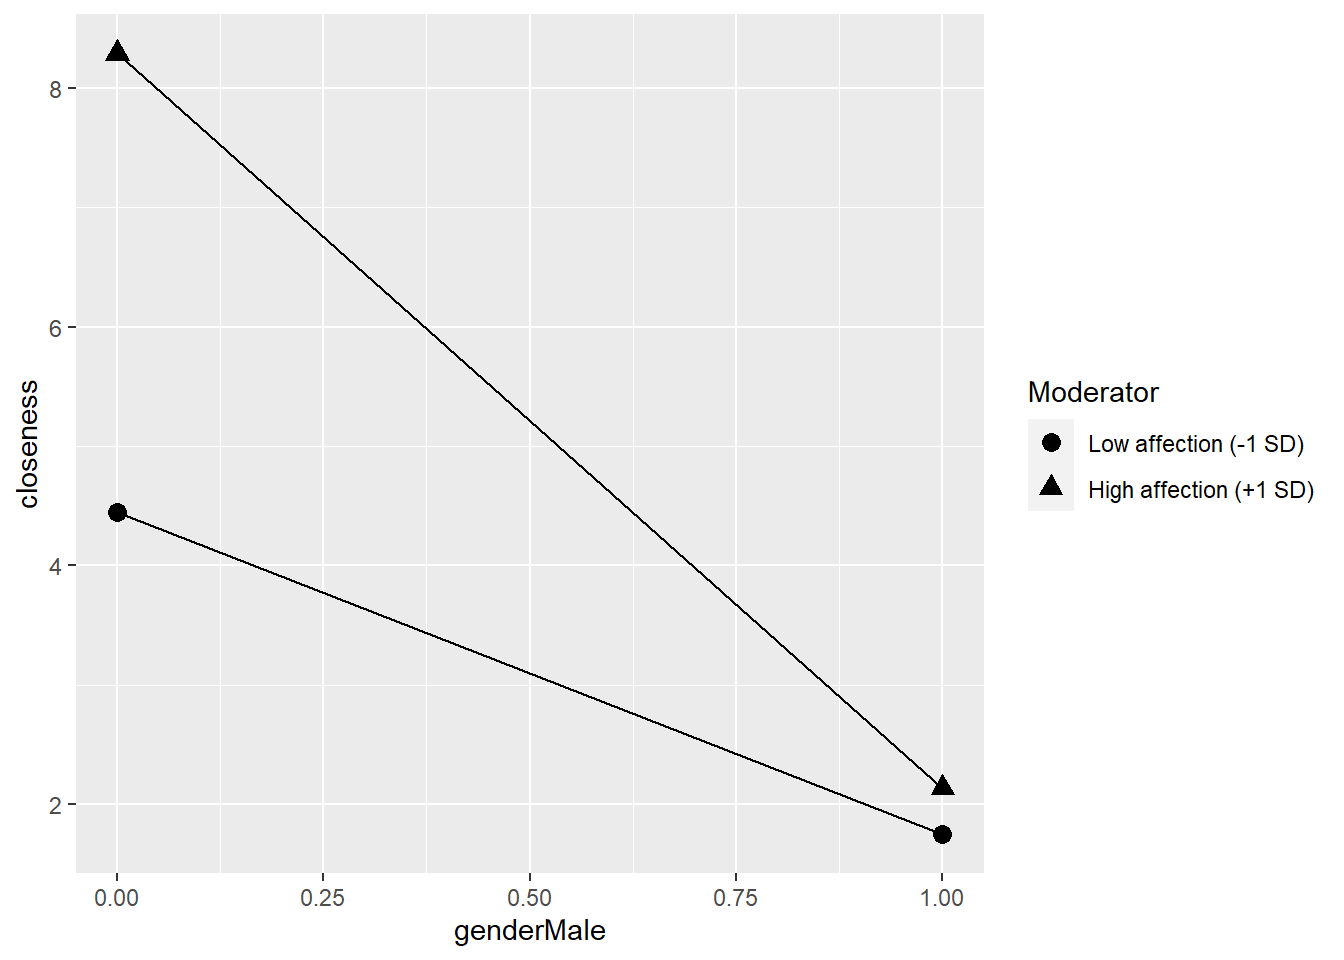
\includegraphics{quick-r-statistics_files/figure-latex/unnamed-chunk-149-1.pdf}

\hypertarget{ux4ee5johnson-neyman-technique}{%
\subsection{以Johnson-Neyman technique}\label{ux4ee5johnson-neyman-technique}}

若要以Johnson-Neyman (JN) technique進一步探究調節效果,需要用R內建的lm()函數來做迴歸。

為了和上面結果相呼應,先產生一個dummy variable: genderD,將男生設為1、女生為0。這邊直接將原dataframe中的gender\_dummy以1去減即可。

\begin{Shaded}
\begin{Highlighting}[]
\NormalTok{cData}\SpecialCharTok{$}\NormalTok{genderD }\OtherTok{\textless{}{-}} \DecValTok{1} \SpecialCharTok{{-}}\NormalTok{ cData}\SpecialCharTok{$}\NormalTok{gender\_dummy}
\end{Highlighting}
\end{Shaded}

若資料中沒有gender\_dummy變項,也可以用plyr套件中的revalue()函數將Male轉為1、Female轉為0,再用as.numeric()函數將之轉為數值。

\begin{Shaded}
\begin{Highlighting}[]
\FunctionTok{library}\NormalTok{(plyr)}
\NormalTok{cData}\SpecialCharTok{$}\NormalTok{D }\OtherTok{\textless{}{-}} \FunctionTok{as.numeric}\NormalTok{(}\FunctionTok{revalue}\NormalTok{(cData}\SpecialCharTok{$}\NormalTok{gender, }\FunctionTok{c}\NormalTok{(}\StringTok{"Male"}\OtherTok{=}\DecValTok{1}\NormalTok{, }\StringTok{\textquotesingle{}Female\textquotesingle{}}\OtherTok{=}\DecValTok{0}\NormalTok{)))}
\end{Highlighting}
\end{Shaded}

將情感(affection)中心化,產生一新的變項affectionC。

\begin{Shaded}
\begin{Highlighting}[]
\NormalTok{cData}\SpecialCharTok{$}\NormalTok{affectionC }\OtherTok{\textless{}{-}} \FunctionTok{c}\NormalTok{(}\FunctionTok{scale}\NormalTok{(cData}\SpecialCharTok{$}\NormalTok{affection, }\AttributeTok{center=}\ConstantTok{TRUE}\NormalTok{, }\AttributeTok{scale=}\ConstantTok{FALSE}\NormalTok{))}
\end{Highlighting}
\end{Shaded}

以affectionC和genderD來預測closeness。

\begin{Shaded}
\begin{Highlighting}[]
\NormalTok{res0 }\OtherTok{\textless{}{-}} \FunctionTok{lm}\NormalTok{(closeness }\SpecialCharTok{\textasciitilde{}}\NormalTok{ affectionC }\SpecialCharTok{+}\NormalTok{ genderD, }\AttributeTok{data=}\NormalTok{cData)}
\FunctionTok{summary}\NormalTok{(res0)}
\end{Highlighting}
\end{Shaded}

\begin{verbatim}
## 
## Call:
## lm(formula = closeness ~ affectionC + genderD, data = cData)
## 
## Residuals:
##     Min      1Q  Median      3Q     Max 
## -3.3733 -0.8598  0.2029  0.8282  3.0625 
## 
## Coefficients:
##             Estimate Std. Error t value Pr(>|t|)    
## (Intercept)  6.29135    0.19168  32.821  < 2e-16 ***
## affectionC   0.26269    0.02963   8.865 3.78e-14 ***
## genderD     -4.46269    0.27189 -16.414  < 2e-16 ***
## ---
## Signif. codes:  0 '***' 0.001 '**' 0.01 '*' 0.05 '.' 0.1 ' ' 1
## 
## Residual standard error: 1.351 on 97 degrees of freedom
## Multiple R-squared:  0.7674, Adjusted R-squared:  0.7626 
## F-statistic:   160 on 2 and 97 DF,  p-value: < 2.2e-16
\end{verbatim}

上述迴歸式加入affectionC*genderD來預測closeness。

\begin{Shaded}
\begin{Highlighting}[]
\NormalTok{res1 }\OtherTok{\textless{}{-}} \FunctionTok{lm}\NormalTok{(closeness }\SpecialCharTok{\textasciitilde{}}\NormalTok{ affectionC }\SpecialCharTok{+}\NormalTok{ genderD }\SpecialCharTok{+}\NormalTok{ affectionC}\SpecialCharTok{*}\NormalTok{genderD, }\AttributeTok{data=}\NormalTok{cData)}
\FunctionTok{summary}\NormalTok{(res1)}
\end{Highlighting}
\end{Shaded}

\begin{verbatim}
## 
## Call:
## lm(formula = closeness ~ affectionC + genderD + affectionC * 
##     genderD, data = cData)
## 
## Residuals:
##      Min       1Q   Median       3Q      Max 
## -2.18730 -0.74369 -0.06341  0.68137  2.89720 
## 
## Coefficients:
##                    Estimate Std. Error t value Pr(>|t|)    
## (Intercept)         6.36873    0.14950  42.601  < 2e-16 ***
## affectionC          0.41746    0.03009  13.874  < 2e-16 ***
## genderD            -4.42985    0.21165 -20.930  < 2e-16 ***
## affectionC:genderD -0.37521    0.04685  -8.009 2.72e-12 ***
## ---
## Signif. codes:  0 '***' 0.001 '**' 0.01 '*' 0.05 '.' 0.1 ' ' 1
## 
## Residual standard error: 1.052 on 96 degrees of freedom
## Multiple R-squared:  0.8606, Adjusted R-squared:  0.8562 
## F-statistic: 197.5 on 3 and 96 DF,  p-value: < 2.2e-16
\end{verbatim}

以anova()比較兩模型。結果同上,有交互作用項的模型有顯著提高解釋力。

\begin{Shaded}
\begin{Highlighting}[]
\FunctionTok{anova}\NormalTok{(res0, res1)}
\end{Highlighting}
\end{Shaded}

\begin{verbatim}
## Analysis of Variance Table
## 
## Model 1: closeness ~ affectionC + genderD
## Model 2: closeness ~ affectionC + genderD + affectionC * genderD
##   Res.Df    RSS Df Sum of Sq     F    Pr(>F)    
## 1     97 177.14                                 
## 2     96 106.19  1    70.948 64.14 2.722e-12 ***
## ---
## Signif. codes:  0 '***' 0.001 '**' 0.01 '*' 0.05 '.' 0.1 ' ' 1
\end{verbatim}

用\href{https://cran.r-project.org/web/packages/processR/index.html}{processR}來做分析。processR目前無法用在最新版的R 4.2.0版,會讓整個R當掉。但R 4.2.0之前的版本沒有問題。

尤其processR在R 4.2.0會有問題,下面的程式碼請自行執行,不再demo。

用modelSummary()來整理迴歸的結果表。

\begin{Shaded}
\begin{Highlighting}[]
\FunctionTok{library}\NormalTok{(processR)}
\FunctionTok{modelsSummary}\NormalTok{(res1)}
\end{Highlighting}
\end{Shaded}

用modelSummary2()來看不同affection(-1SD、0、+1SD)和gender(0、1)組合的closeness。

\begin{Shaded}
\begin{Highlighting}[]
\FunctionTok{modSummary2}\NormalTok{(res1, }\AttributeTok{rangemode=}\DecValTok{1}\NormalTok{)}
\end{Highlighting}
\end{Shaded}

用modSummary3()來看conditional effect。結果顯示,當affectionC為0時,slope為-4.43;affectionC為+1 SD時,slope為-2.70;affectionC為-1 SD時,slope為-6.16。

\begin{Shaded}
\begin{Highlighting}[]
\FunctionTok{modSummary3}\NormalTok{(res1, }\AttributeTok{X=}\StringTok{\textquotesingle{}genderD\textquotesingle{}}\NormalTok{, }\AttributeTok{W=}\StringTok{\textquotesingle{}affectionC\textquotesingle{}}\NormalTok{, }\AttributeTok{rangemode=}\DecValTok{1}\NormalTok{)}
\end{Highlighting}
\end{Shaded}

\hypertarget{ux4ee5rockchalkux5957ux4ef6ux5206ux6790}{%
\subsubsection{以rockchalk套件分析}\label{ux4ee5rockchalkux5957ux4ef6ux5206ux6790}}

以rockchalk套件的plotSlopes()來畫上述conditional effect的圖。

\begin{Shaded}
\begin{Highlighting}[]
\FunctionTok{library}\NormalTok{(rockchalk)}
\NormalTok{ps }\OtherTok{\textless{}{-}} \FunctionTok{plotSlopes}\NormalTok{(res1, }\AttributeTok{plotx=}\StringTok{"genderD"}\NormalTok{, }\AttributeTok{modx=}\StringTok{"affectionC"}\NormalTok{, }\AttributeTok{modxVals=}\StringTok{"std.dev"}\NormalTok{)}
\end{Highlighting}
\end{Shaded}

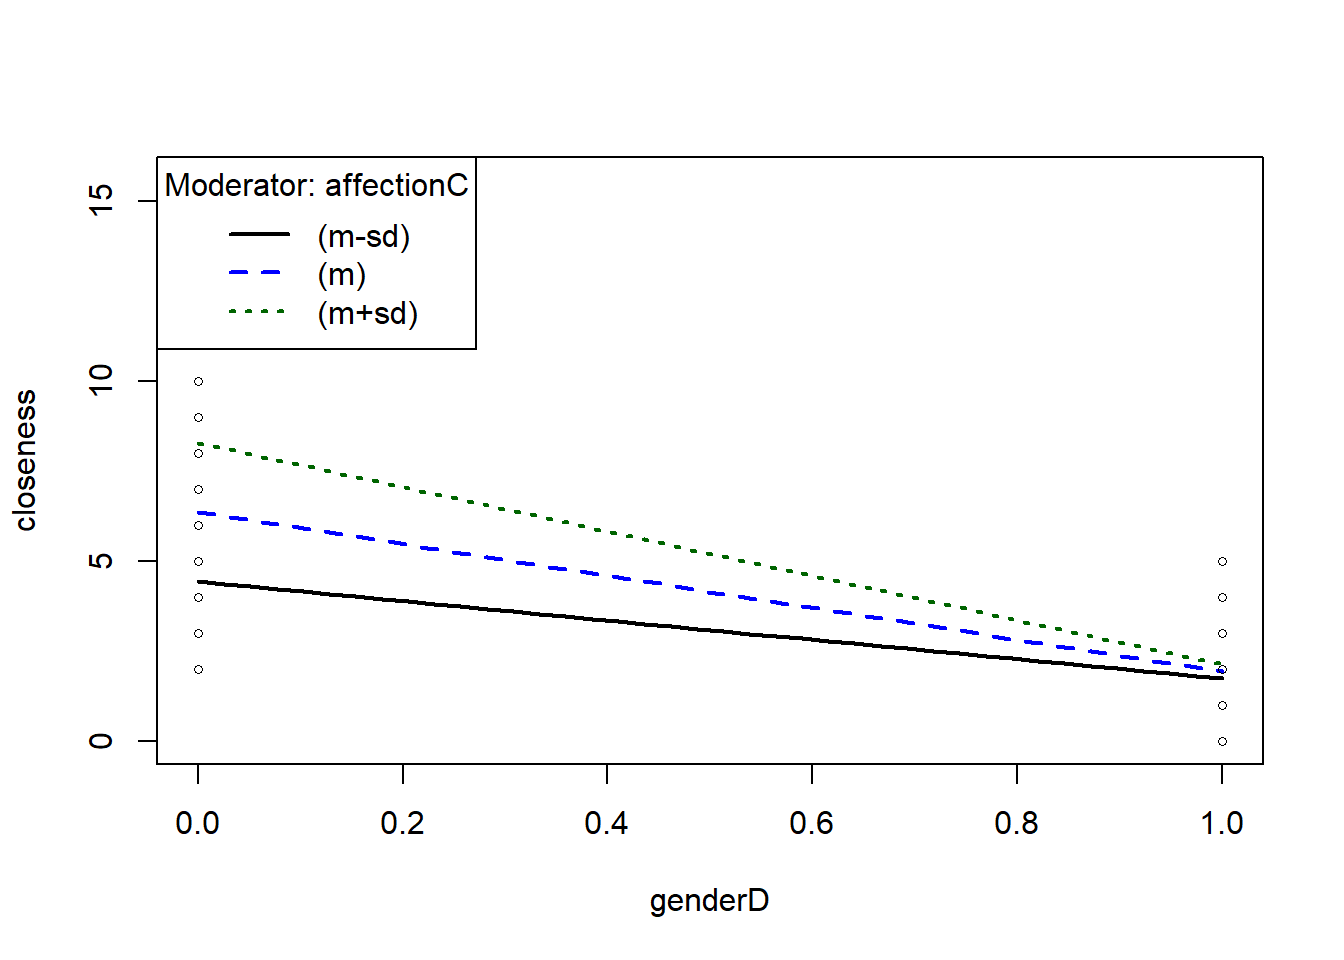
\includegraphics{quick-r-statistics_files/figure-latex/unnamed-chunk-159-1.pdf}

Johnson-Neyman (JN) technique: 檢驗各affectC下的conditional effect,其slope是否顯著。

\begin{Shaded}
\begin{Highlighting}[]
\NormalTok{ts }\OtherTok{\textless{}{-}} \FunctionTok{testSlopes}\NormalTok{(ps)}
\end{Highlighting}
\end{Shaded}

\begin{verbatim}
## Values of affectionC OUTSIDE this interval:
##         lo         hi 
## -15.931548  -9.238178 
## cause the slope of (b1 + b2*affectionC)genderD to be statistically significant
\end{verbatim}

\begin{Shaded}
\begin{Highlighting}[]
\FunctionTok{plot}\NormalTok{(ts)}
\end{Highlighting}
\end{Shaded}

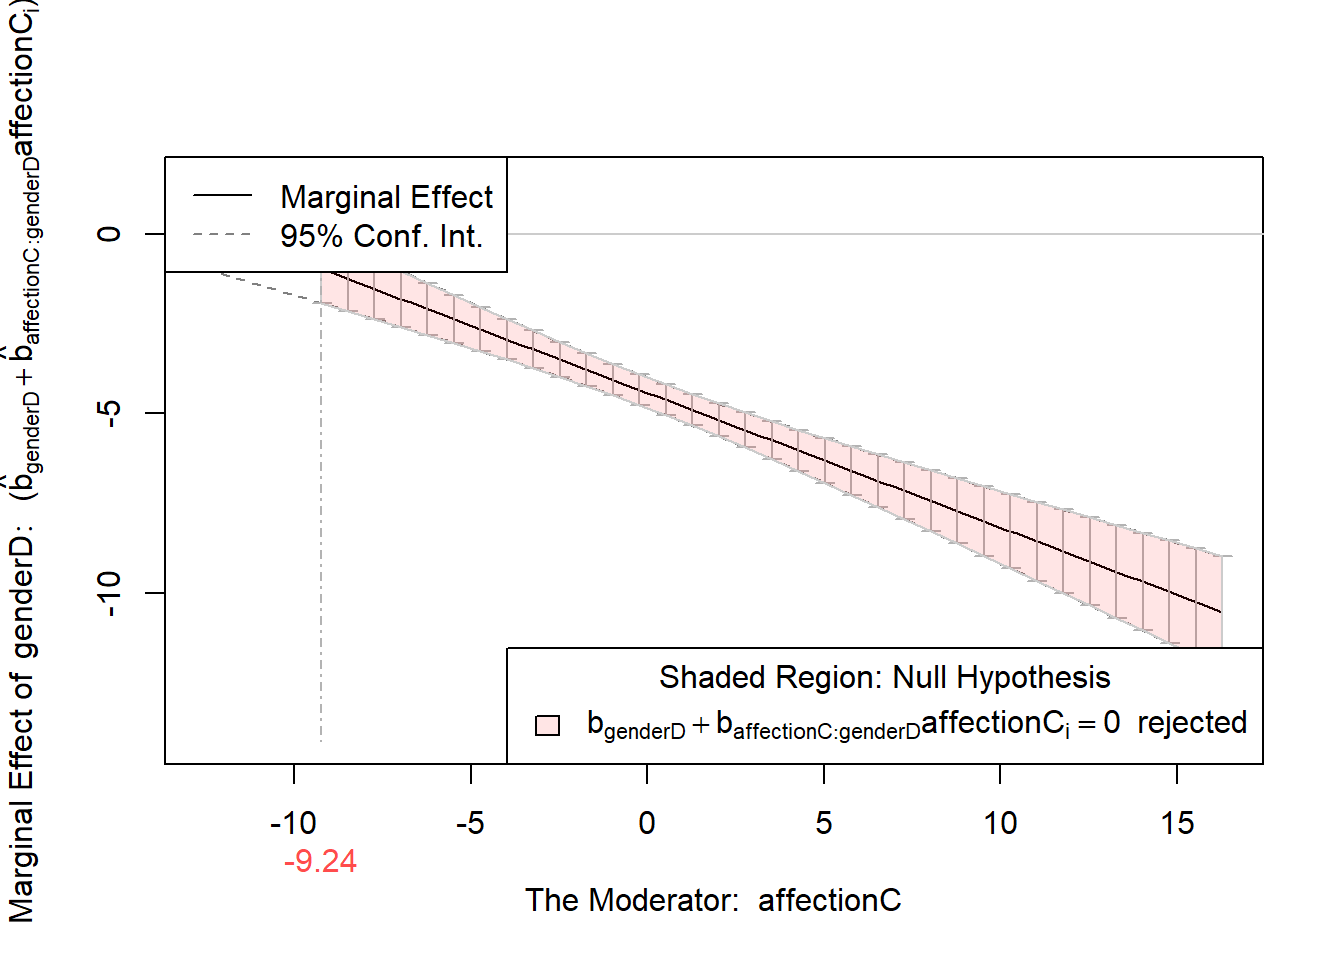
\includegraphics{quick-r-statistics_files/figure-latex/unnamed-chunk-160-1.pdf}

\hypertarget{ux4ee5interacionsux5957ux4ef6ux5206ux6790}{%
\subsubsection{以interacions套件分析}\label{ux4ee5interacionsux5957ux4ef6ux5206ux6790}}

\href{https://cran.r-project.org/web/packages/interactions/readme/README.html}{interactions套件}也提供很好的視覺化圖表功能,可用來看conditional effect與Johnson-Neyman分析。

畫conditional effect的圖,含資料點。

\begin{Shaded}
\begin{Highlighting}[]
\FunctionTok{library}\NormalTok{(interactions)}
\FunctionTok{interact\_plot}\NormalTok{(res1, }\AttributeTok{pred =}\NormalTok{ genderD, }\AttributeTok{modx =}\NormalTok{ affectionC, }\AttributeTok{plot.points =} \ConstantTok{TRUE}\NormalTok{)}
\end{Highlighting}
\end{Shaded}

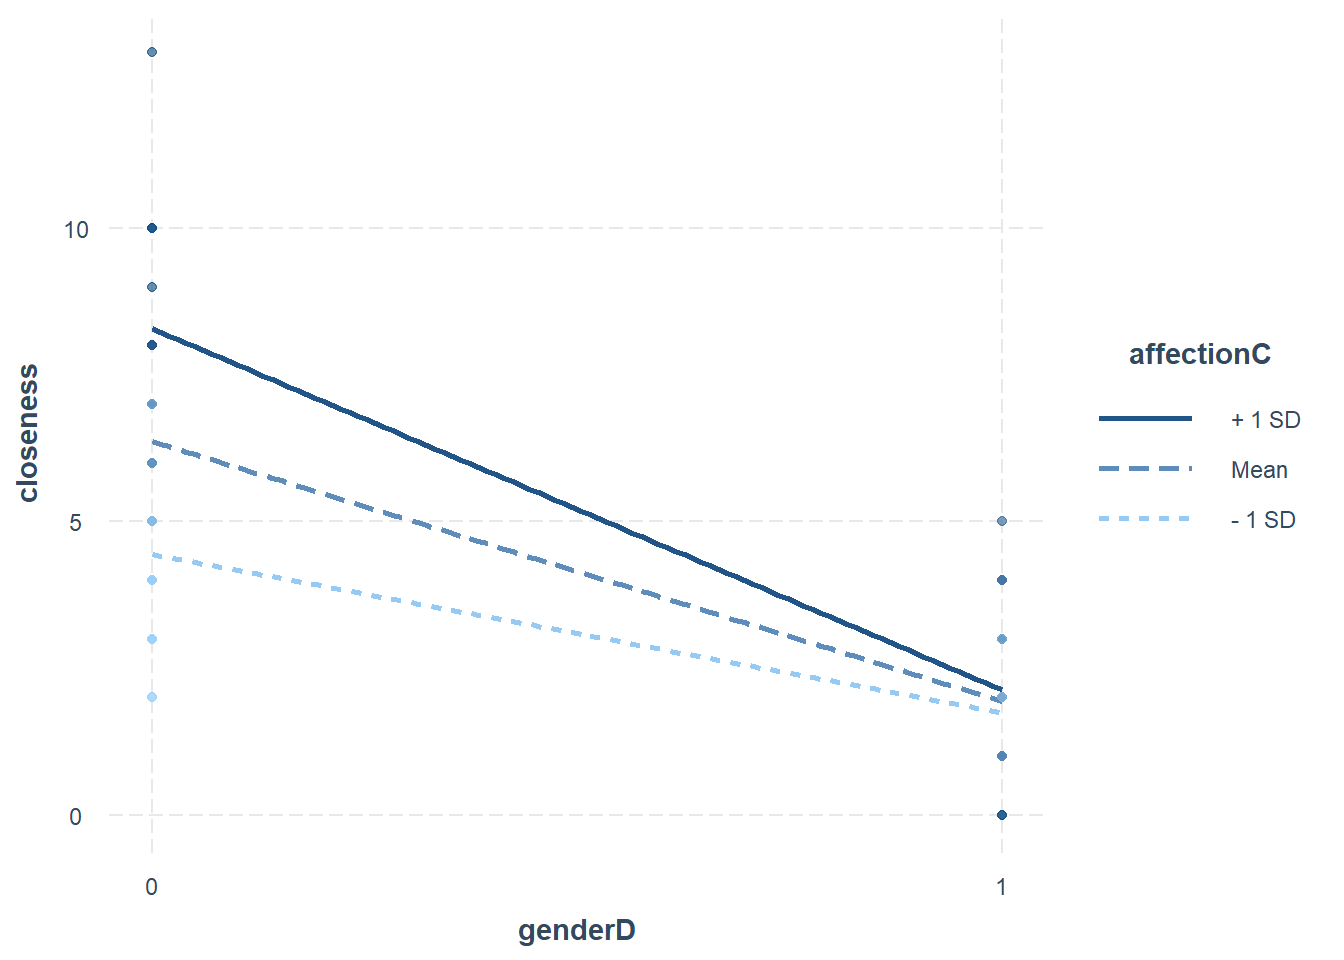
\includegraphics{quick-r-statistics_files/figure-latex/unnamed-chunk-161-1.pdf}

畫conditional effect的圖,含信賴區間。

\begin{Shaded}
\begin{Highlighting}[]
\FunctionTok{interact\_plot}\NormalTok{(res1, }\AttributeTok{pred =}\NormalTok{ genderD, }\AttributeTok{modx =}\NormalTok{ affectionC, }\AttributeTok{interval =} \ConstantTok{TRUE}\NormalTok{)}
\end{Highlighting}
\end{Shaded}

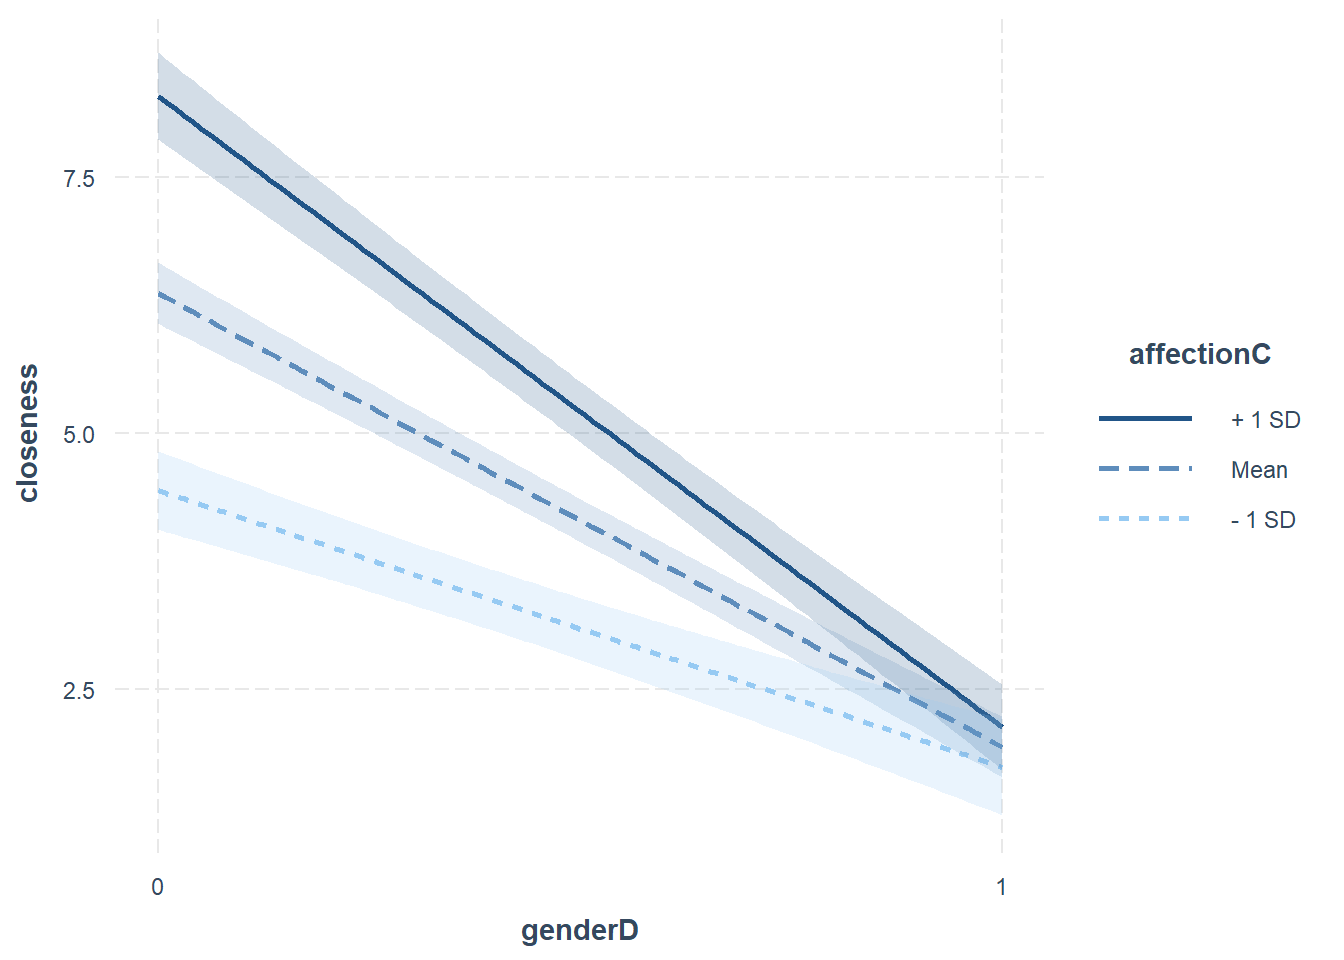
\includegraphics{quick-r-statistics_files/figure-latex/unnamed-chunk-162-1.pdf}

做Johnson-Neyman分析。

\begin{Shaded}
\begin{Highlighting}[]
\FunctionTok{sim\_slopes}\NormalTok{(res1, }\AttributeTok{pred =}\NormalTok{ genderD, }\AttributeTok{modx =}\NormalTok{ affectionC, }\AttributeTok{jnplot =} \ConstantTok{TRUE}\NormalTok{)}
\end{Highlighting}
\end{Shaded}

\begin{verbatim}
## JOHNSON-NEYMAN INTERVAL 
## 
## When affectionC is OUTSIDE the interval [-15.93, -9.24], the slope of
## genderD is p < .05.
## 
## Note: The range of observed values of affectionC is [-10.12, 13.88]
\end{verbatim}

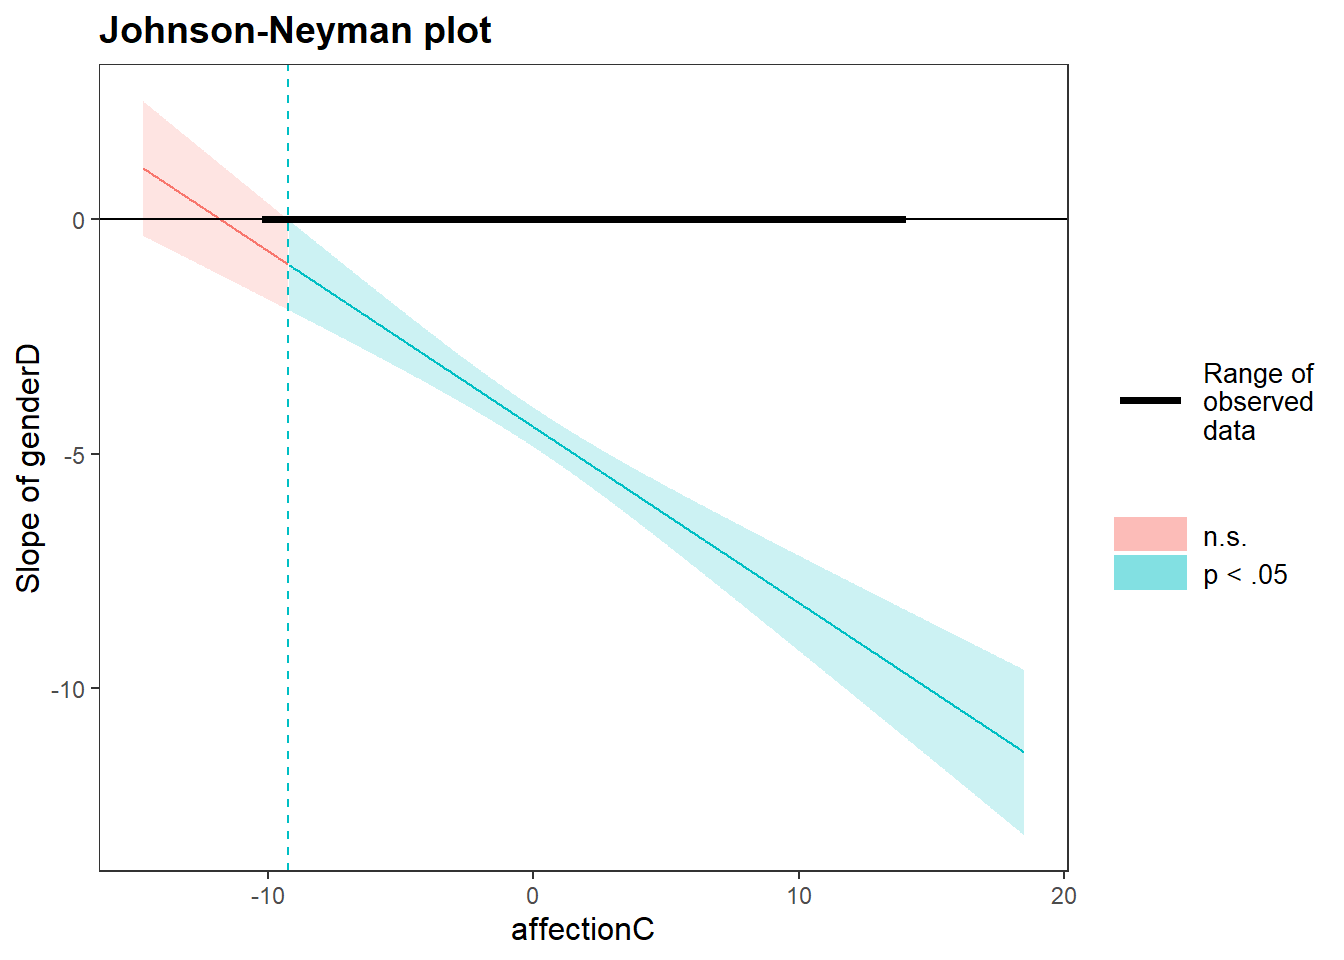
\includegraphics{quick-r-statistics_files/figure-latex/unnamed-chunk-163-1.pdf}

\begin{verbatim}
## SIMPLE SLOPES ANALYSIS 
## 
## Slope of genderD when affectionC = -4.61066e+00 (- 1 SD): 
## 
##    Est.   S.E.   t val.      p
## ------- ------ -------- ------
##   -2.70   0.31    -8.84   0.00
## 
## Slope of genderD when affectionC =  7.81597e-16 (Mean): 
## 
##    Est.   S.E.   t val.      p
## ------- ------ -------- ------
##   -4.43   0.21   -20.93   0.00
## 
## Slope of genderD when affectionC =  4.61066e+00 (+ 1 SD): 
## 
##    Est.   S.E.   t val.      p
## ------- ------ -------- ------
##   -6.16   0.30   -20.57   0.00
\end{verbatim}

或是用john\_neyman()函數來做圖。

\begin{Shaded}
\begin{Highlighting}[]
\FunctionTok{johnson\_neyman}\NormalTok{(}\AttributeTok{model =}\NormalTok{ res1, }\AttributeTok{pred =}\NormalTok{ genderD, }\AttributeTok{modx =}\NormalTok{ affectionC)}
\end{Highlighting}
\end{Shaded}

\begin{verbatim}
## JOHNSON-NEYMAN INTERVAL 
## 
## When affectionC is OUTSIDE the interval [-15.93, -9.24], the slope of
## genderD is p < .05.
## 
## Note: The range of observed values of affectionC is [-10.12, 13.88]
\end{verbatim}

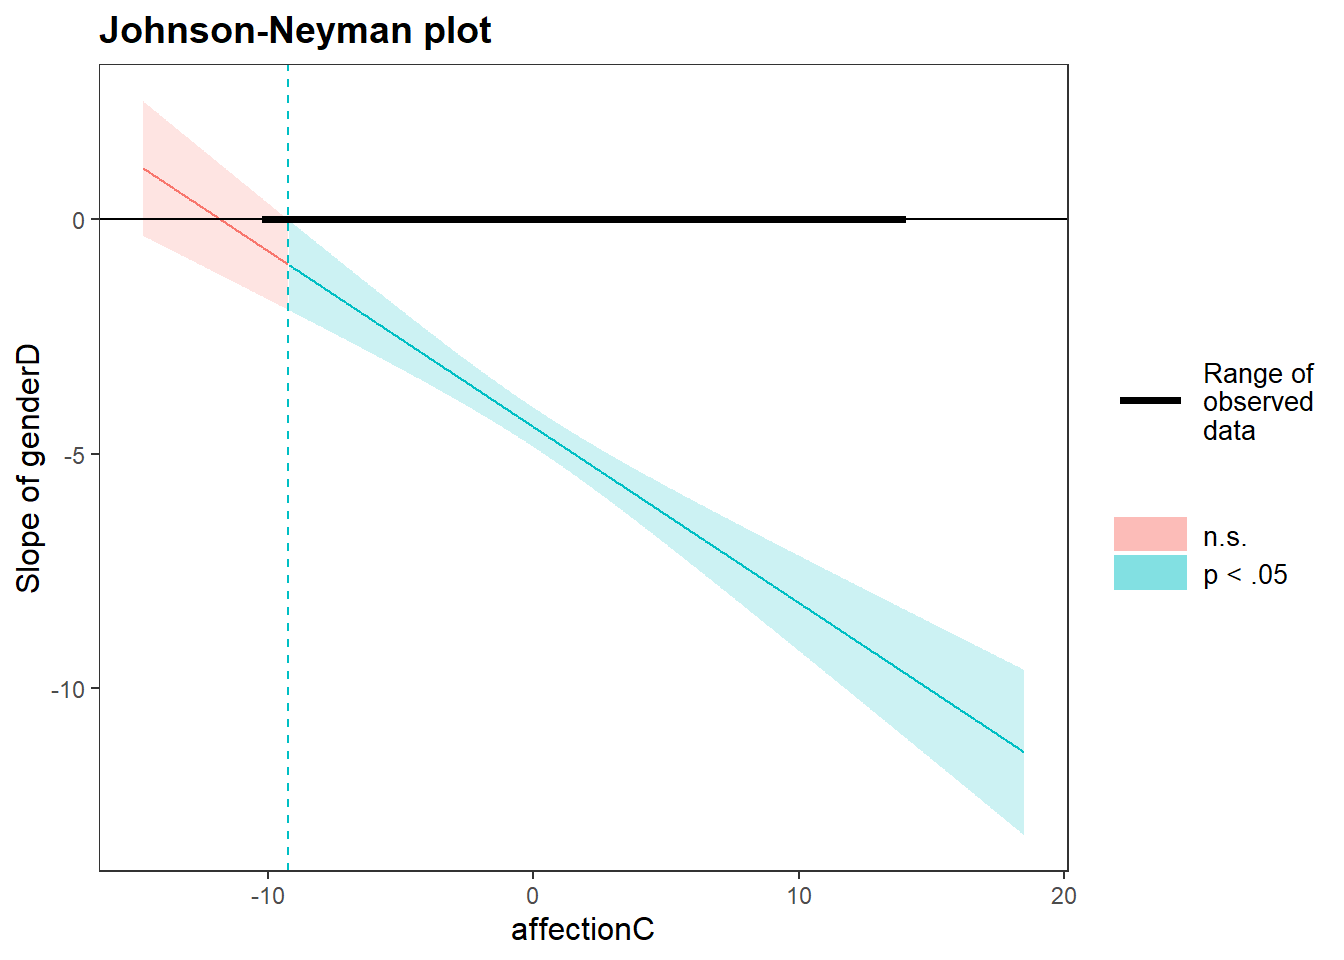
\includegraphics{quick-r-statistics_files/figure-latex/unnamed-chunk-164-1.pdf}

\hypertarget{ux7528process-macroux4f86ux5206ux6790}{%
\subsubsection{用process macro來分析}\label{ux7528process-macroux4f86ux5206ux6790}}

若是習慣使用Andrew Hayes發展的process macro,可先到\href{https://www.processmacro.org/index.html}{process的網站}下載檔案。解壓縮後直接執行process.R。可用source(`檔案路徑')來執行,或全選後按run執行,前者會快一些,因為不會列印出一堆文字。

\begin{Shaded}
\begin{Highlighting}[]
\FunctionTok{source}\NormalTok{(}\StringTok{\textquotesingle{}D:}\SpecialCharTok{\textbackslash{}\textbackslash{}}\StringTok{Dropbox}\SpecialCharTok{\textbackslash{}\textbackslash{}}\StringTok{processR}\SpecialCharTok{\textbackslash{}\textbackslash{}}\StringTok{PROCESS v4.1 for R}\SpecialCharTok{\textbackslash{}\textbackslash{}}\StringTok{process.R\textquotesingle{}}\NormalTok{)}
\end{Highlighting}
\end{Shaded}

同上的model,以process來做分析。model=1是調節模型,jn=1表示要執行Johnson--Neyman Technique分析。center=2表示僅將連續變項中心化,plot=1表示要輸出Data for visualizing the conditional effect of the focal predictor。

\begin{Shaded}
\begin{Highlighting}[]
\FunctionTok{process}\NormalTok{(}\AttributeTok{data=}\NormalTok{cData,}\AttributeTok{y=}\StringTok{"closeness"}\NormalTok{,}\AttributeTok{x=}\StringTok{"genderD"}\NormalTok{,}\AttributeTok{w=}\StringTok{"affection"}\NormalTok{, }\AttributeTok{model=}\DecValTok{1}\NormalTok{, }\AttributeTok{center=}\DecValTok{2}\NormalTok{, }\AttributeTok{jn=}\DecValTok{1}\NormalTok{, }\AttributeTok{plot=}\DecValTok{1}\NormalTok{)}
\end{Highlighting}
\end{Shaded}

\hypertarget{mediation}{%
\chapter{中介效果分析}\label{mediation}}

本單元介紹如何以R語言做中介效果分析。

\hypertarget{ux8b80ux5165ux8cc7ux6599ux4e26ux756bux5716ux6aa2ux8996-1}{%
\section{讀入資料並畫圖檢視}\label{ux8b80ux5165ux8cc7ux6599ux4e26ux756bux5716ux6aa2ux8996-1}}

以JASP提供的\href{https://jasp-stats.org/wp-content/uploads/2020/03/mediation.csv}{mediation.csv}為例,以R做分析。

此資料為一項假設的研究資料。在研究中以量表詢問了父母對孩子的養育採取自由放任態度的程度(laissez\_faire)、孩子的獨立程度(independence)、以及孩子的探索行為量(exploration)。研究假設為:強烈的自由放任態度對孩子的獨立性有正向的效果。其可能的機制為,自由放任的態度會影響孩子的探索行為量,進而影響其獨立性。意即,探索是態度對獨立性影響的中介變項。

以read.table()獨入資料。

\begin{Shaded}
\begin{Highlighting}[]
\NormalTok{mData }\OtherTok{\textless{}{-}} \FunctionTok{read.table}\NormalTok{(}\StringTok{"mediation.csv"}\NormalTok{, }\AttributeTok{header=}\ConstantTok{TRUE}\NormalTok{, }\AttributeTok{sep=}\StringTok{","}\NormalTok{)}
\end{Highlighting}
\end{Shaded}

\begin{tabular}{r|r|r|r}
\hline
laissez\_faire & exploration & independence & disobedience\\
\hline
7 & 4 & 8 & 2\\
\hline
6 & 2 & 6 & 3\\
\hline
12 & 3 & 7 & 4\\
\hline
14 & 4 & 7 & 5\\
\hline
17 & 6 & 11 & 3\\
\hline
19 & 6 & 10 & 5\\
\hline
\end{tabular}

\hypertarget{ux4ee5rux5167ux5efaux7684lmux51fdux6578ux4f86ux505aux5206ux6790}{%
\section{以R內建的lm函數來做分析}\label{ux4ee5rux5167ux5efaux7684lmux51fdux6578ux4f86ux505aux5206ux6790}}

\hypertarget{ux7e3dux6548ux679cux6aa2ux9a57}{%
\subsection{總效果檢驗}\label{ux7e3dux6548ux679cux6aa2ux9a57}}

以laissez\_faire預測independence,模型解釋力顯著。

\begin{Shaded}
\begin{Highlighting}[]
\NormalTok{fit }\OtherTok{\textless{}{-}} \FunctionTok{lm}\NormalTok{(independence}\SpecialCharTok{\textasciitilde{}}\NormalTok{laissez\_faire, }\AttributeTok{data=}\NormalTok{mData)}
\FunctionTok{summary}\NormalTok{(fit)}
\end{Highlighting}
\end{Shaded}

\begin{verbatim}
## 
## Call:
## lm(formula = independence ~ laissez_faire, data = mData)
## 
## Residuals:
##     Min      1Q  Median      3Q     Max 
## -6.6202 -1.5732 -0.0493  1.4424  6.5051 
## 
## Coefficients:
##               Estimate Std. Error t value Pr(>|t|)    
## (Intercept)    5.21426    0.61960   8.415 3.27e-13 ***
## laissez_faire  0.23433    0.05151   4.549 1.54e-05 ***
## ---
## Signif. codes:  0 '***' 0.001 '**' 0.01 '*' 0.05 '.' 0.1 ' ' 1
## 
## Residual standard error: 2.363 on 98 degrees of freedom
## Multiple R-squared:  0.1744, Adjusted R-squared:  0.1659 
## F-statistic:  20.7 on 1 and 98 DF,  p-value: 1.544e-05
\end{verbatim}

\hypertarget{ux4ee5ux9810ux6e2cux9805ux4f86ux9810ux6e2cux4e2dux4ecbux8b8aux9805}{%
\subsection{以預測項來預測中介變項}\label{ux4ee5ux9810ux6e2cux9805ux4f86ux9810ux6e2cux4e2dux4ecbux8b8aux9805}}

以laissez\_faire預測exploration,效果亦顯著。

\begin{Shaded}
\begin{Highlighting}[]
\NormalTok{fita }\OtherTok{\textless{}{-}} \FunctionTok{lm}\NormalTok{(exploration }\SpecialCharTok{\textasciitilde{}}\NormalTok{ laissez\_faire, }\AttributeTok{data=}\NormalTok{mData)}
\FunctionTok{summary}\NormalTok{(fita)}
\end{Highlighting}
\end{Shaded}

\begin{verbatim}
## 
## Call:
## lm(formula = exploration ~ laissez_faire, data = mData)
## 
## Residuals:
##      Min       1Q   Median       3Q      Max 
## -2.12610 -0.76207 -0.08926  0.60196  2.56513 
## 
## Coefficients:
##               Estimate Std. Error t value Pr(>|t|)    
## (Intercept)    2.18840    0.27134   8.065 1.84e-12 ***
## laissez_faire  0.17281    0.02256   7.661 1.33e-11 ***
## ---
## Signif. codes:  0 '***' 0.001 '**' 0.01 '*' 0.05 '.' 0.1 ' ' 1
## 
## Residual standard error: 1.035 on 98 degrees of freedom
## Multiple R-squared:  0.3746, Adjusted R-squared:  0.3682 
## F-statistic: 58.69 on 1 and 98 DF,  p-value: 1.333e-11
\end{verbatim}

\hypertarget{ux4e2dux4ecbux8b8aux9805ux8207ux9810ux6e2cux9805ux5171ux540cux9810ux6e2cux4f9dux8b8aux9805}{%
\subsection{中介變項與預測項共同預測依變項}\label{ux4e2dux4ecbux8b8aux9805ux8207ux9810ux6e2cux9805ux5171ux540cux9810ux6e2cux4f9dux8b8aux9805}}

\begin{Shaded}
\begin{Highlighting}[]
\NormalTok{fitb }\OtherTok{\textless{}{-}} \FunctionTok{lm}\NormalTok{(independence }\SpecialCharTok{\textasciitilde{}}\NormalTok{ exploration }\SpecialCharTok{+}\NormalTok{ laissez\_faire, }\AttributeTok{data=}\NormalTok{mData)}
\FunctionTok{summary}\NormalTok{(fitb)}
\end{Highlighting}
\end{Shaded}

\begin{verbatim}
## 
## Call:
## lm(formula = independence ~ exploration + laissez_faire, data = mData)
## 
## Residuals:
##     Min      1Q  Median      3Q     Max 
## -4.1713 -0.7227 -0.0016  0.8303  2.8300 
## 
## Coefficients:
##               Estimate Std. Error t value Pr(>|t|)    
## (Intercept)    0.84015    0.38843   2.163 0.033003 *  
## exploration    1.99877    0.11211  17.829  < 2e-16 ***
## laissez_faire -0.11107    0.03165  -3.509 0.000684 ***
## ---
## Signif. codes:  0 '***' 0.001 '**' 0.01 '*' 0.05 '.' 0.1 ' ' 1
## 
## Residual standard error: 1.148 on 97 degrees of freedom
## Multiple R-squared:  0.807,  Adjusted R-squared:  0.803 
## F-statistic: 202.7 on 2 and 97 DF,  p-value: < 2.2e-16
\end{verbatim}

\hypertarget{ux4e2dux4ecbux6548ux679cux6aa2ux9a57}{%
\subsection{中介效果檢驗}\label{ux4e2dux4ecbux6548ux679cux6aa2ux9a57}}

以stargazer套件的stargazer()函數來看三變項之間的關係。

\begin{Shaded}
\begin{Highlighting}[]
\FunctionTok{library}\NormalTok{(stargazer)}
\FunctionTok{stargazer}\NormalTok{(fit, fita, fitb, }\AttributeTok{type =} \StringTok{"text"}\NormalTok{, }\AttributeTok{title =} \StringTok{"Baron and Kenny Method"}\NormalTok{)}
\end{Highlighting}
\end{Shaded}

\begin{verbatim}
## 
## Baron and Kenny Method
## =========================================================================================
##                                              Dependent variable:                         
##                     ---------------------------------------------------------------------
##                          independence           exploration            independence      
##                              (1)                    (2)                     (3)          
## -----------------------------------------------------------------------------------------
## exploration                                                              1.999***        
##                                                                           (0.112)        
##                                                                                          
## laissez_faire              0.234***               0.173***               -0.111***       
##                            (0.052)                (0.023)                 (0.032)        
##                                                                                          
## Constant                   5.214***               2.188***                0.840**        
##                            (0.620)                (0.271)                 (0.388)        
##                                                                                          
## -----------------------------------------------------------------------------------------
## Observations                 100                    100                     100          
## R2                          0.174                  0.375                   0.807         
## Adjusted R2                 0.166                  0.368                   0.803         
## Residual Std. Error    2.363 (df = 98)        1.035 (df = 98)         1.148 (df = 97)    
## F Statistic         20.696*** (df = 1; 98) 58.688*** (df = 1; 98) 202.746*** (df = 2; 97)
## =========================================================================================
## Note:                                                         *p<0.1; **p<0.05; ***p<0.01
\end{verbatim}

以multilevel套件的sobel()函數來做Sobel test檢驗中介效果,看indirect effect是否顯著。

\begin{Shaded}
\begin{Highlighting}[]
\FunctionTok{library}\NormalTok{(multilevel)}
\FunctionTok{sobel}\NormalTok{(mData}\SpecialCharTok{$}\NormalTok{laissez\_faire, mData}\SpecialCharTok{$}\NormalTok{exploration, mData}\SpecialCharTok{$}\NormalTok{independence)}
\end{Highlighting}
\end{Shaded}

\begin{verbatim}
## $`Mod1: Y~X`
##              Estimate Std. Error  t value     Pr(>|t|)
## (Intercept) 5.2142586 0.61960212 8.415495 3.267909e-13
## pred        0.2343293 0.05150847 4.549335 1.543558e-05
## 
## $`Mod2: Y~X+M`
##               Estimate Std. Error   t value     Pr(>|t|)
## (Intercept)  0.8401457 0.38842542  2.162952 3.300257e-02
## pred        -0.1110699 0.03165459 -3.508809 6.841546e-04
## med          1.9987717 0.11210741 17.829078 2.255937e-32
## 
## $`Mod3: M~X`
##              Estimate Std. Error  t value     Pr(>|t|)
## (Intercept) 2.1884004  0.2713435 8.065056 1.842647e-12
## pred        0.1728057  0.0225572 7.660779 1.333137e-11
## 
## $Indirect.Effect
## [1] 0.3453992
## 
## $SE
## [1] 0.04907255
## 
## $z.value
## [1] 7.038542
## 
## $N
## [1] 100
\end{verbatim}

以bda套件的mediation.test()函數來做Sobel mediation test,變項的順序依序為mv、iv、dv。

\begin{Shaded}
\begin{Highlighting}[]
\FunctionTok{library}\NormalTok{(bda)}
\FunctionTok{mediation.test}\NormalTok{(mData}\SpecialCharTok{$}\NormalTok{exploration, mData}\SpecialCharTok{$}\NormalTok{laissez\_faire, mData}\SpecialCharTok{$}\NormalTok{independence)}
\end{Highlighting}
\end{Shaded}

\begin{verbatim}
##                Sobel       Aroian      Goodman
## z.value 7.038542e+00 7.029215e+00 7.047906e+00
## p.value 1.942620e-12 2.076993e-12 1.816300e-12
\end{verbatim}

\hypertarget{ux4ee5psychux5957ux4ef6ux4f86ux5206ux6790}{%
\section{以psych套件來分析}\label{ux4ee5psychux5957ux4ef6ux4f86ux5206ux6790}}

用psych套件的mediate()函數來做中介效果的分析。

\begin{Shaded}
\begin{Highlighting}[]
\FunctionTok{library}\NormalTok{(psych)}
\NormalTok{m1 }\OtherTok{\textless{}{-}} \FunctionTok{mediate}\NormalTok{(independence }\SpecialCharTok{\textasciitilde{}}\NormalTok{ laissez\_faire }\SpecialCharTok{+}\NormalTok{ (exploration), }\AttributeTok{data=}\NormalTok{mData, }\AttributeTok{n.iter =} \DecValTok{10000}\NormalTok{) }
\end{Highlighting}
\end{Shaded}

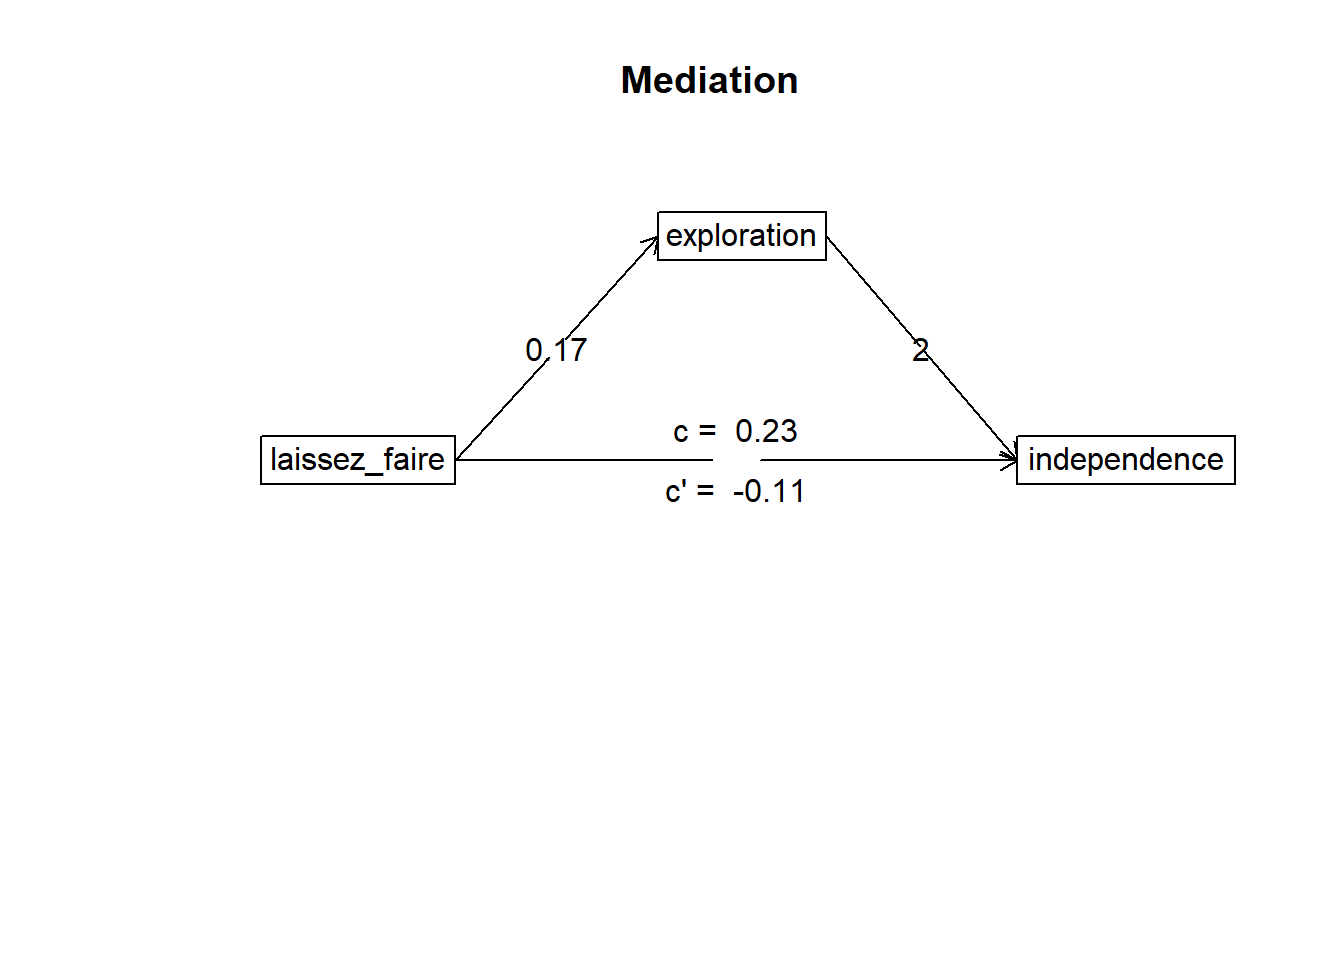
\includegraphics{quick-r-statistics_files/figure-latex/unnamed-chunk-177-1.pdf}

\begin{Shaded}
\begin{Highlighting}[]
\FunctionTok{summary}\NormalTok{(m1)}
\end{Highlighting}
\end{Shaded}

\begin{verbatim}
## Call: mediate(y = independence ~ laissez_faire + (exploration), data = mData, 
##     n.iter = 10000)
## 
## Direct effect estimates (traditional regression)    (c') X + M on Y 
##               independence   se     t df     Prob
## Intercept             0.84 0.39  2.16 97 3.30e-02
## laissez_faire        -0.11 0.03 -3.51 97 6.84e-04
## exploration           2.00 0.11 17.83 97 2.26e-32
## 
## R = 0.9 R2 = 0.81   F = 202.75 on 2 and 97 DF   p-value:  2.26e-35 
## 
##  Total effect estimates (c) (X on Y) 
##               independence   se    t df     Prob
## Intercept             5.21 0.62 8.42 98 3.27e-13
## laissez_faire         0.23 0.05 4.55 98 1.54e-05
## 
##  'a'  effect estimates (X on M) 
##               exploration   se    t df     Prob
## Intercept            2.19 0.27 8.07 98 1.84e-12
## laissez_faire        0.17 0.02 7.66 98 1.33e-11
## 
##  'b'  effect estimates (M on Y controlling for X) 
##             independence   se     t df     Prob
## exploration            2 0.11 17.83 97 2.26e-32
## 
##  'ab'  effect estimates (through all  mediators)
##               independence boot   sd lower upper
## laissez_faire         0.35 0.35 0.05  0.26  0.44
\end{verbatim}

畫圖呈現。

\begin{Shaded}
\begin{Highlighting}[]
\FunctionTok{mediate.diagram}\NormalTok{(m1)}
\end{Highlighting}
\end{Shaded}

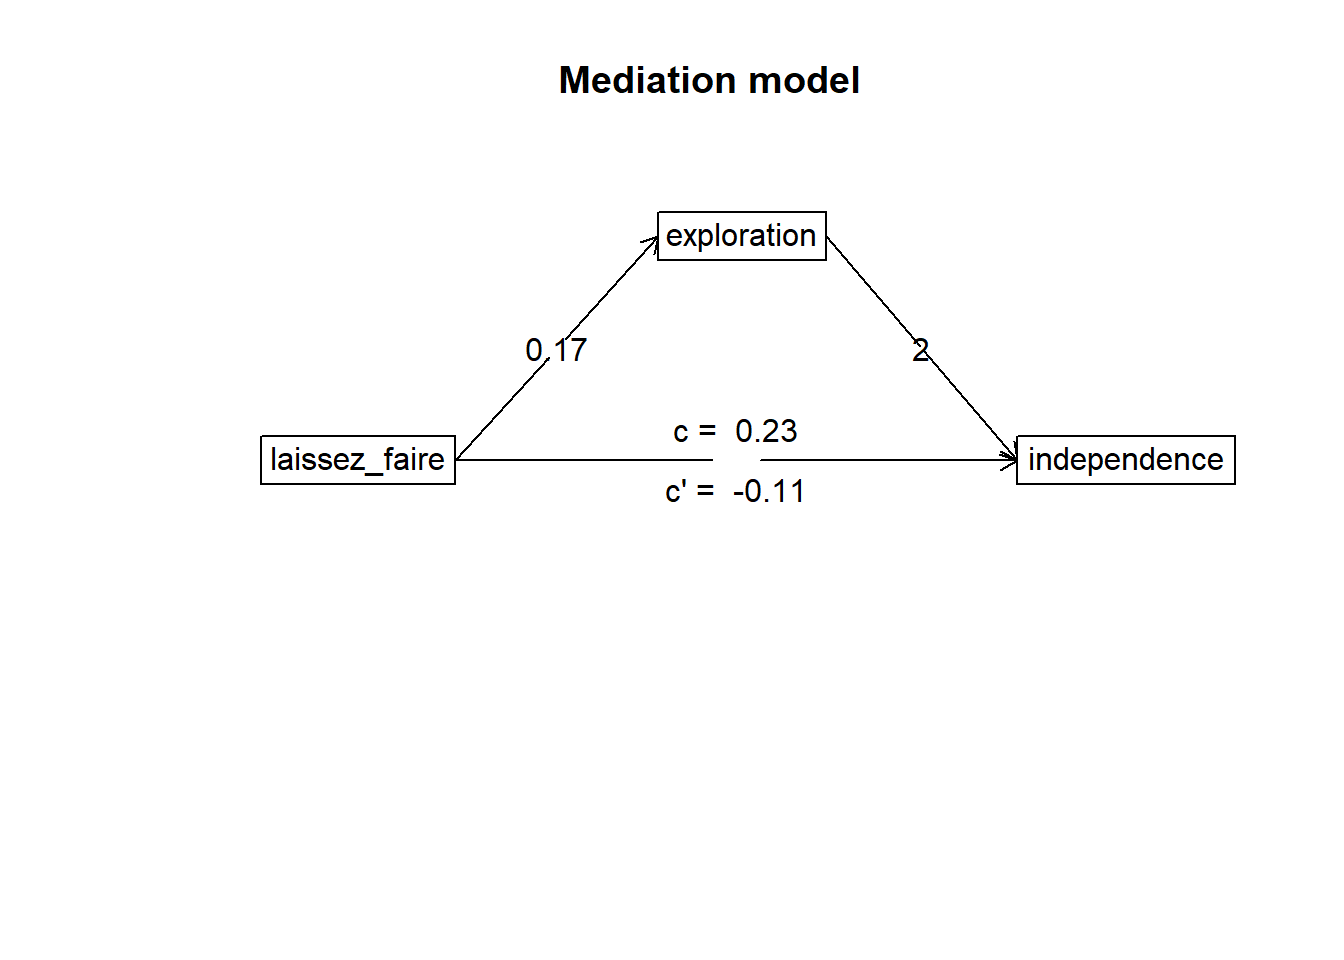
\includegraphics{quick-r-statistics_files/figure-latex/unnamed-chunk-178-1.pdf}

\hypertarget{ux4ee5mediationux5957ux4ef6ux4f86ux505aux5206ux6790}{%
\section{以mediation套件來做分析}\label{ux4ee5mediationux5957ux4ef6ux4f86ux505aux5206ux6790}}

以mediation套件來做中介效果的分析。

\begin{Shaded}
\begin{Highlighting}[]
\FunctionTok{library}\NormalTok{(mediation)}
\NormalTok{fitM }\OtherTok{\textless{}{-}} \FunctionTok{lm}\NormalTok{(exploration }\SpecialCharTok{\textasciitilde{}}\NormalTok{ laissez\_faire, }\AttributeTok{data=}\NormalTok{mData)}
\NormalTok{fitY }\OtherTok{\textless{}{-}} \FunctionTok{lm}\NormalTok{(independence }\SpecialCharTok{\textasciitilde{}}\NormalTok{ laissez\_faire }\SpecialCharTok{+}\NormalTok{ exploration, }\AttributeTok{data=}\NormalTok{mData)}
\FunctionTok{summary}\NormalTok{(fitM)}
\end{Highlighting}
\end{Shaded}

\begin{verbatim}
## 
## Call:
## lm(formula = exploration ~ laissez_faire, data = mData)
## 
## Residuals:
##      Min       1Q   Median       3Q      Max 
## -2.12610 -0.76207 -0.08926  0.60196  2.56513 
## 
## Coefficients:
##               Estimate Std. Error t value Pr(>|t|)    
## (Intercept)    2.18840    0.27134   8.065 1.84e-12 ***
## laissez_faire  0.17281    0.02256   7.661 1.33e-11 ***
## ---
## Signif. codes:  0 '***' 0.001 '**' 0.01 '*' 0.05 '.' 0.1 ' ' 1
## 
## Residual standard error: 1.035 on 98 degrees of freedom
## Multiple R-squared:  0.3746, Adjusted R-squared:  0.3682 
## F-statistic: 58.69 on 1 and 98 DF,  p-value: 1.333e-11
\end{verbatim}

\begin{Shaded}
\begin{Highlighting}[]
\FunctionTok{summary}\NormalTok{(fitY)}
\end{Highlighting}
\end{Shaded}

\begin{verbatim}
## 
## Call:
## lm(formula = independence ~ laissez_faire + exploration, data = mData)
## 
## Residuals:
##     Min      1Q  Median      3Q     Max 
## -4.1713 -0.7227 -0.0016  0.8303  2.8300 
## 
## Coefficients:
##               Estimate Std. Error t value Pr(>|t|)    
## (Intercept)    0.84015    0.38843   2.163 0.033003 *  
## laissez_faire -0.11107    0.03165  -3.509 0.000684 ***
## exploration    1.99877    0.11211  17.829  < 2e-16 ***
## ---
## Signif. codes:  0 '***' 0.001 '**' 0.01 '*' 0.05 '.' 0.1 ' ' 1
## 
## Residual standard error: 1.148 on 97 degrees of freedom
## Multiple R-squared:  0.807,  Adjusted R-squared:  0.803 
## F-statistic: 202.7 on 2 and 97 DF,  p-value: < 2.2e-16
\end{verbatim}

中介分析的結果如下表。其中,ACME為Average Causal Mediation Effect (indirect effects),ADE為Average Direct Effect,Prop. Mediated為ACME/Total Effect的比率。由結果可知,laissez\_faire可預測independence (b = 0.233, p \textless{} .001),而exploration在此關係中具有中介效果(b = 0.344, p \textless{} .001), laissez\_faire有直接效果(b = -0.111, p \textless{} .001)。

\begin{Shaded}
\begin{Highlighting}[]
\NormalTok{fitMed }\OtherTok{\textless{}{-}} \FunctionTok{mediate}\NormalTok{(fitM, fitY, }\AttributeTok{treat=}\StringTok{"laissez\_faire"}\NormalTok{, }\AttributeTok{mediator=}\StringTok{"exploration"}\NormalTok{)}
\FunctionTok{summary}\NormalTok{(fitMed)}
\end{Highlighting}
\end{Shaded}

\begin{verbatim}
## 
## Causal Mediation Analysis 
## 
## Quasi-Bayesian Confidence Intervals
## 
##                Estimate 95% CI Lower 95% CI Upper p-value    
## ACME              0.346        0.256         0.44  <2e-16 ***
## ADE              -0.111       -0.172        -0.05  <2e-16 ***
## Total Effect      0.235        0.130         0.33  <2e-16 ***
## Prop. Mediated    1.480        1.163         2.10  <2e-16 ***
## ---
## Signif. codes:  0 '***' 0.001 '**' 0.01 '*' 0.05 '.' 0.1 ' ' 1
## 
## Sample Size Used: 100 
## 
## 
## Simulations: 1000
\end{verbatim}

效果圖示。

\begin{Shaded}
\begin{Highlighting}[]
\FunctionTok{plot}\NormalTok{(fitMed)}
\end{Highlighting}
\end{Shaded}

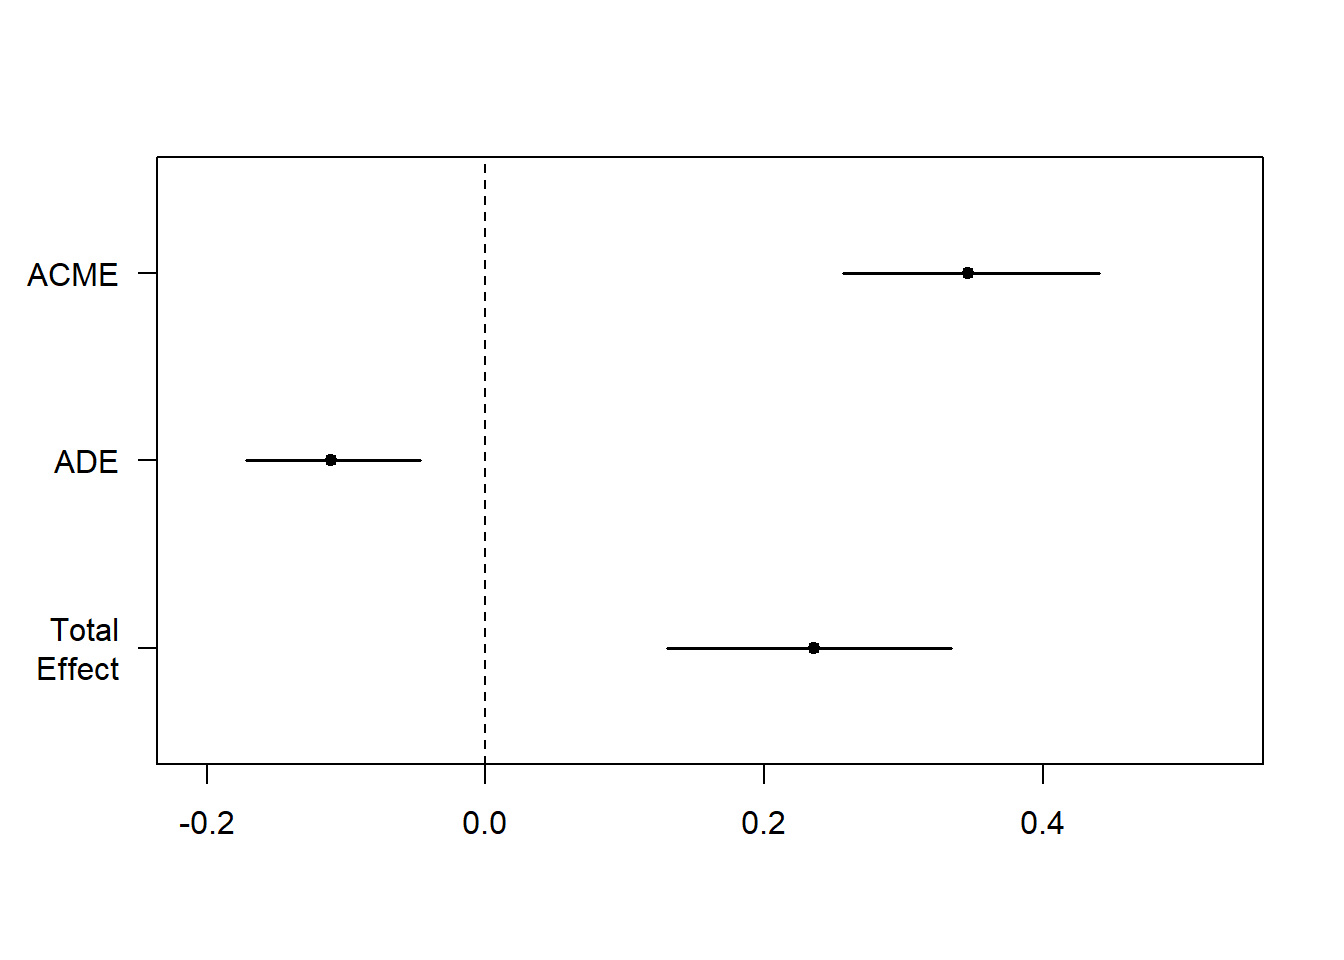
\includegraphics{quick-r-statistics_files/figure-latex/unnamed-chunk-181-1.pdf}

\hypertarget{bootstrappingux6cd5}{%
\subsection{Bootstrapping法}\label{bootstrappingux6cd5}}

若為小樣本、資料違反常態,可用Bootstrapping法。

\begin{Shaded}
\begin{Highlighting}[]
\NormalTok{fitMedBoot }\OtherTok{\textless{}{-}} \FunctionTok{mediate}\NormalTok{(fitM, fitY, }\AttributeTok{boot=}\ConstantTok{TRUE}\NormalTok{, }\AttributeTok{sims=}\DecValTok{999}\NormalTok{, }\AttributeTok{treat=}\StringTok{"laissez\_faire"}\NormalTok{, }\AttributeTok{mediator=}\StringTok{"exploration"}\NormalTok{)}
\FunctionTok{summary}\NormalTok{(fitMedBoot)}
\end{Highlighting}
\end{Shaded}

\begin{verbatim}
## 
## Causal Mediation Analysis 
## 
## Nonparametric Bootstrap Confidence Intervals with the Percentile Method
## 
##                Estimate 95% CI Lower 95% CI Upper p-value    
## ACME              0.345        0.262         0.44  <2e-16 ***
## ADE              -0.111       -0.172        -0.05  <2e-16 ***
## Total Effect      0.234        0.150         0.33  <2e-16 ***
## Prop. Mediated    1.474        1.202         1.95  <2e-16 ***
## ---
## Signif. codes:  0 '***' 0.001 '**' 0.01 '*' 0.05 '.' 0.1 ' ' 1
## 
## Sample Size Used: 100 
## 
## 
## Simulations: 999
\end{verbatim}

\begin{Shaded}
\begin{Highlighting}[]
\FunctionTok{plot}\NormalTok{(fitMedBoot)}
\end{Highlighting}
\end{Shaded}

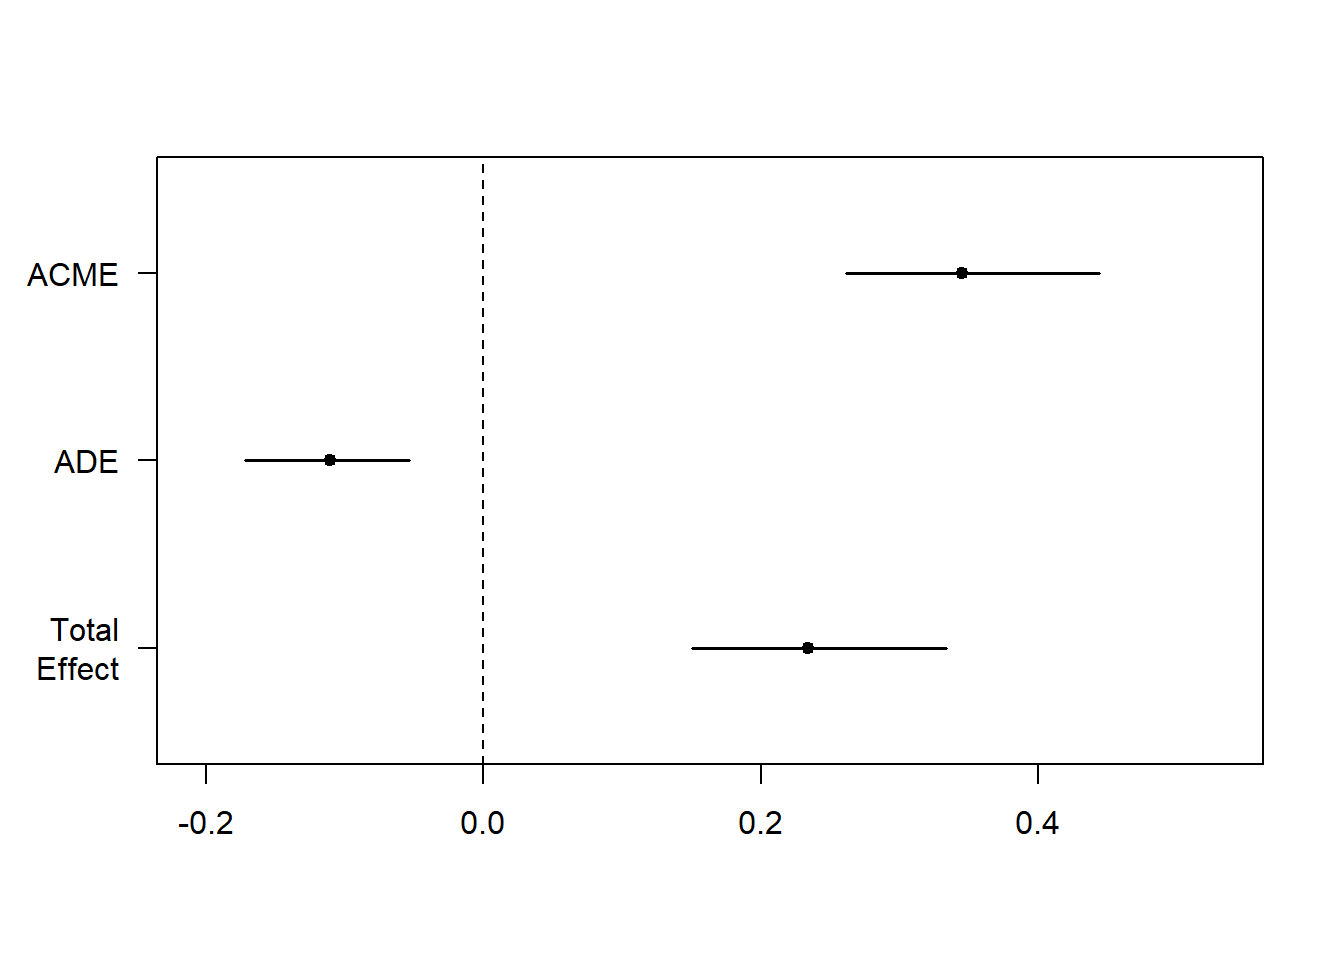
\includegraphics{quick-r-statistics_files/figure-latex/unnamed-chunk-182-1.pdf}

\hypertarget{multisheets}{%
\chapter{多個EXCEL檔的資料匯整與分析}\label{multisheets}}

以R整理多個excel檔的資料並加以統計 - 以學生學習成效資料為例。

\hypertarget{ux5b78ux7fd2ux6210ux6548ux5206ux6790}{%
\section{學習成效分析}\label{ux5b78ux7fd2ux6210ux6548ux5206ux6790}}

下載\href{https://drive.google.com/drive/u/0/folders/1-eNELkxrsLIdgfEX4S3nZIvmhnC00fEt}{學習成效原始資料},並統計2017\textasciitilde2020年所有課程的學習成效。

先將所有檔案放到工作目錄下的一個資料夾(例如TableDemo資料夾)內,並在R中設定好工作目錄。(你也可以將此資料夾設為工作目錄,這邊因為Rmarkdown的關係,所以這樣設定。)

\begin{Shaded}
\begin{Highlighting}[]
\FunctionTok{setwd}\NormalTok{(}\StringTok{"D:}\SpecialCharTok{\textbackslash{}\textbackslash{}}\StringTok{Dropbox}\SpecialCharTok{\textbackslash{}\textbackslash{}}\StringTok{Working}\SpecialCharTok{\textbackslash{}\textbackslash{}}\StringTok{教師社群"}\NormalTok{)}
\end{Highlighting}
\end{Shaded}

\hypertarget{ux8b80ux5165ux55aeux4e00ux5de5ux4f5cux8868ux4e26ux62bdux53d6ux6240ux9700ux8cc7ux6599}{%
\section{讀入單一工作表並抽取所需資料}\label{ux8b80ux5165ux55aeux4e00ux5de5ux4f5cux8868ux4e26ux62bdux53d6ux6240ux9700ux8cc7ux6599}}

先讀入單一工作表,並抽取學習成效的資料。

以readxl套件,讀取UG-2017.xlsx的sheet 1。因為表格中沒有column name,readxl會出現警告訊息,不想看到的話可以加上suppressMessages()。

\begin{Shaded}
\begin{Highlighting}[]
\FunctionTok{library}\NormalTok{(readxl)}
\FunctionTok{suppressMessages}\NormalTok{(qData }\OtherTok{\textless{}{-}} \FunctionTok{read\_xlsx}\NormalTok{(}\StringTok{"TableDemo}\SpecialCharTok{\textbackslash{}\textbackslash{}}\StringTok{UG{-}2017.xlsx"}\NormalTok{, }\DecValTok{1}\NormalTok{))}
\end{Highlighting}
\end{Shaded}

以which()找出「三、學習成效評估」的位置,為「學習成效評估表」的起始位置;並以整個表格長度做為「學習成效評估表」的終點位置。

\begin{Shaded}
\begin{Highlighting}[]
\NormalTok{index\_start }\OtherTok{\textless{}{-}} \FunctionTok{which}\NormalTok{(qData}\SpecialCharTok{$}\StringTok{\textasciigrave{}}\AttributeTok{一、教學意見量化結果}\StringTok{\textasciigrave{}}\SpecialCharTok{==}\StringTok{"三、學習成效評估"}\NormalTok{)}
\NormalTok{index\_end }\OtherTok{\textless{}{-}} \FunctionTok{length}\NormalTok{(qData}\SpecialCharTok{$}\StringTok{\textasciigrave{}}\AttributeTok{一、教學意見量化結果}\StringTok{\textasciigrave{}}\NormalTok{)}
\end{Highlighting}
\end{Shaded}

抓出「學習成效評估表」的所有數值。

\begin{Shaded}
\begin{Highlighting}[]
\FunctionTok{library}\NormalTok{(dplyr)}
\NormalTok{myData }\OtherTok{\textless{}{-}} \FunctionTok{slice}\NormalTok{(qData,index\_start}\SpecialCharTok{:}\NormalTok{index\_end)  }
\CommentTok{\# myData \textless{}{-} qData[index\_start:index\_end,]  \#相當於這樣寫 }
\NormalTok{myData}
\end{Highlighting}
\end{Shaded}

\begin{tabular}{l|l|l|l|l|l|l|l}
\hline
一、教學意見量化結果 & ...2 & ...3 & ...4 & ...5 & ...6 & ...7 & ...8\\
\hline
三、學習成效評估 & NA & NA & NA & NA & NA & NA & NA\\
\hline
NA & NA & NA & NA & NA & NA & NA & NA\\
\hline
題目 & 答題人數 & (5分)非常符合 & (4分)符合 & (3分)尚可 & (2分)不符合 & (1分)非常不符合 & 單題指標\\
\hline
1.能獲得本科目(領域)之知識 & 21 & 12 & 9 & 0 & 0 & 0 & 4.57\\
\hline
NA & NA & 57.00\% & 43.00\% & 0\% & 0\% & 0\% & NA\\
\hline
題目 & 答題人數 & (5分)非常符合 & (4分)符合 & (3分)尚可 & (2分)不符合 & (1分)非常不符合 & 單題指標\\
\hline
2.能獲得本科目(領域)之重要概念 & 21 & 12 & 7 & 2 & 0 & 0 & 4.48\\
\hline
NA & NA & 57.00\% & 33.00\% & 10.00\% & 0\% & 0\% & NA\\
\hline
題目 & 答題人數 & (5分)非常符合 & (4分)符合 & (3分)尚可 & (2分)不符合 & (1分)非常不符合 & 單題指標\\
\hline
5.能學到專業領域的重要技術 & 21 & 12 & 5 & 4 & 0 & 0 & 4.38\\
\hline
NA & NA & 57.00\% & 24.00\% & 19.00\% & 0\% & 0\% & NA\\
\hline
題目 & 答題人數 & (5分)非常符合 & (4分)符合 & (3分)尚可 & (2分)不符合 & (1分)非常不符合 & 單題指標\\
\hline
7.能提升實務操作的能力 & 21 & 12 & 5 & 4 & 0 & 0 & 4.38\\
\hline
NA & NA & 57.00\% & 24.00\% & 19.00\% & 0\% & 0\% & NA\\
\hline
題目 & 答題人數 & (5分)非常符合 & (4分)符合 & (3分)尚可 & (2分)不符合 & (1分)非常不符合 & 單題指標\\
\hline
15.能提升資料蒐集分析與運用能力 & 21 & 12 & 8 & 1 & 0 & 0 & 4.52\\
\hline
NA & NA & 57.00\% & 38.00\% & 5.00\% & 0\% & 0\% & NA\\
\hline
本課程學習成效平均分數 & NA & NA & NA & NA & NA & NA & 4.47\\
\hline
\end{tabular}

刪除NA的列。

\begin{Shaded}
\begin{Highlighting}[]
\NormalTok{data1 }\OtherTok{\textless{}{-}} \FunctionTok{na.omit}\NormalTok{(myData) }\CommentTok{\# way1}
\DocumentationTok{\#\# data1 \textless{}{-} myData[complete.cases(myData), ] \#way2}
\DocumentationTok{\#\# data1 \textless{}{-} myData[complete.cases(myData[ , 1:8]),] \#way3: 可刪除部份data}

\NormalTok{data1}
\end{Highlighting}
\end{Shaded}

\begin{tabular}{l|l|l|l|l|l|l|l}
\hline
一、教學意見量化結果 & ...2 & ...3 & ...4 & ...5 & ...6 & ...7 & ...8\\
\hline
題目 & 答題人數 & (5分)非常符合 & (4分)符合 & (3分)尚可 & (2分)不符合 & (1分)非常不符合 & 單題指標\\
\hline
1.能獲得本科目(領域)之知識 & 21 & 12 & 9 & 0 & 0 & 0 & 4.57\\
\hline
題目 & 答題人數 & (5分)非常符合 & (4分)符合 & (3分)尚可 & (2分)不符合 & (1分)非常不符合 & 單題指標\\
\hline
2.能獲得本科目(領域)之重要概念 & 21 & 12 & 7 & 2 & 0 & 0 & 4.48\\
\hline
題目 & 答題人數 & (5分)非常符合 & (4分)符合 & (3分)尚可 & (2分)不符合 & (1分)非常不符合 & 單題指標\\
\hline
5.能學到專業領域的重要技術 & 21 & 12 & 5 & 4 & 0 & 0 & 4.38\\
\hline
題目 & 答題人數 & (5分)非常符合 & (4分)符合 & (3分)尚可 & (2分)不符合 & (1分)非常不符合 & 單題指標\\
\hline
7.能提升實務操作的能力 & 21 & 12 & 5 & 4 & 0 & 0 & 4.38\\
\hline
題目 & 答題人數 & (5分)非常符合 & (4分)符合 & (3分)尚可 & (2分)不符合 & (1分)非常不符合 & 單題指標\\
\hline
15.能提升資料蒐集分析與運用能力 & 21 & 12 & 8 & 1 & 0 & 0 & 4.52\\
\hline
\end{tabular}

刪掉每個題目表格的title列。

\begin{Shaded}
\begin{Highlighting}[]
\NormalTok{data2 }\OtherTok{\textless{}{-}} \FunctionTok{subset}\NormalTok{(data1, }\StringTok{\textasciigrave{}}\AttributeTok{一、教學意見量化結果}\StringTok{\textasciigrave{}}\SpecialCharTok{!=}\StringTok{"題目"}\NormalTok{, }\AttributeTok{select=}\FunctionTok{c}\NormalTok{(}\DecValTok{1}\NormalTok{,}\DecValTok{2}\NormalTok{,}\DecValTok{8}\NormalTok{))}
\NormalTok{data2}
\end{Highlighting}
\end{Shaded}

\begin{tabular}{l|l|l}
\hline
一、教學意見量化結果 & ...2 & ...8\\
\hline
1.能獲得本科目(領域)之知識 & 21 & 4.57\\
\hline
2.能獲得本科目(領域)之重要概念 & 21 & 4.48\\
\hline
5.能學到專業領域的重要技術 & 21 & 4.38\\
\hline
7.能提升實務操作的能力 & 21 & 4.38\\
\hline
15.能提升資料蒐集分析與運用能力 & 21 & 4.52\\
\hline
\end{tabular}

\hypertarget{ux7c21ux5316ux7a0bux5f0f}{%
\subsection{簡化程式}\label{ux7c21ux5316ux7a0bux5f0f}}

以\%\textgreater\%來簡化程式,讓程式更具可讀性,也不需在中間過程多存出變項。意即,只要將qData放入後,即可產生tb1 (即上述data2)。

\begin{Shaded}
\begin{Highlighting}[]
\NormalTok{tb1 }\OtherTok{\textless{}{-}} \FunctionTok{slice}\NormalTok{(qData,index\_start}\SpecialCharTok{:}\NormalTok{index\_end) }\SpecialCharTok{\%\textgreater{}\%}
  \FunctionTok{na.omit}\NormalTok{() }\SpecialCharTok{\%\textgreater{}\%}
  \FunctionTok{subset}\NormalTok{(}\StringTok{\textasciigrave{}}\AttributeTok{一、教學意見量化結果}\StringTok{\textasciigrave{}}\SpecialCharTok{!=}\StringTok{"題目"}\NormalTok{, }\AttributeTok{select=}\FunctionTok{c}\NormalTok{(}\DecValTok{1}\NormalTok{,}\DecValTok{2}\NormalTok{,}\DecValTok{8}\NormalTok{))}
\end{Highlighting}
\end{Shaded}

\hypertarget{ux5bebux6210ux51fdux6578}{%
\subsection{寫成函數}\label{ux5bebux6210ux51fdux6578}}

將上述步驟寫成函數anal\_Teach\_Q,只要給予filename和nSheet即可傳回tb1。

\begin{Shaded}
\begin{Highlighting}[]
\FunctionTok{library}\NormalTok{(readxl)}
\FunctionTok{library}\NormalTok{(dplyr)}

\NormalTok{anal\_Teach\_Q }\OtherTok{\textless{}{-}} \ControlFlowTok{function}\NormalTok{(filename, nSheet)\{}
  \FunctionTok{suppressMessages}\NormalTok{(qData }\OtherTok{\textless{}{-}} \FunctionTok{read\_xlsx}\NormalTok{(filename, nSheet))}
\NormalTok{  index\_start }\OtherTok{\textless{}{-}} \FunctionTok{which}\NormalTok{(qData}\SpecialCharTok{$}\StringTok{\textasciigrave{}}\AttributeTok{一、教學意見量化結果}\StringTok{\textasciigrave{}}\SpecialCharTok{==}\StringTok{"三、學習成效評估"}\NormalTok{)}
\NormalTok{  index\_end }\OtherTok{\textless{}{-}} \FunctionTok{length}\NormalTok{(qData}\SpecialCharTok{$}\StringTok{\textasciigrave{}}\AttributeTok{一、教學意見量化結果}\StringTok{\textasciigrave{}}\NormalTok{)}
\NormalTok{  tb1 }\OtherTok{\textless{}{-}} \FunctionTok{slice}\NormalTok{(qData,index\_start}\SpecialCharTok{:}\NormalTok{index\_end) }\SpecialCharTok{\%\textgreater{}\%}
    \FunctionTok{na.omit}\NormalTok{() }\SpecialCharTok{\%\textgreater{}\%}
    \FunctionTok{subset}\NormalTok{(}\StringTok{\textasciigrave{}}\AttributeTok{一、教學意見量化結果}\StringTok{\textasciigrave{}}\SpecialCharTok{!=}\StringTok{"題目"}\NormalTok{, }\AttributeTok{select=}\FunctionTok{c}\NormalTok{(}\DecValTok{1}\NormalTok{,}\DecValTok{2}\NormalTok{,}\DecValTok{8}\NormalTok{))}
  \FunctionTok{return}\NormalTok{(tb1)}
\NormalTok{\}}
\end{Highlighting}
\end{Shaded}

呼叫anal\_Teach\_Q,分析「UG-2017.xlsx」的sheet1。

\begin{Shaded}
\begin{Highlighting}[]
\NormalTok{thisfilename }\OtherTok{\textless{}{-}} \StringTok{"TableDemo}\SpecialCharTok{\textbackslash{}\textbackslash{}}\StringTok{UG{-}2017.xlsx"}
\NormalTok{nSheet }\OtherTok{\textless{}{-}} \DecValTok{1}
\NormalTok{tb1 }\OtherTok{\textless{}{-}} \FunctionTok{anal\_Teach\_Q}\NormalTok{(thisfilename, nSheet)}
\NormalTok{tb1}
\end{Highlighting}
\end{Shaded}

\begin{tabular}{l|l|l}
\hline
一、教學意見量化結果 & ...2 & ...8\\
\hline
1.能獲得本科目(領域)之知識 & 21 & 4.57\\
\hline
2.能獲得本科目(領域)之重要概念 & 21 & 4.48\\
\hline
5.能學到專業領域的重要技術 & 21 & 4.38\\
\hline
7.能提升實務操作的能力 & 21 & 4.38\\
\hline
15.能提升資料蒐集分析與運用能力 & 21 & 4.52\\
\hline
\end{tabular}

\hypertarget{ux8b80ux53d6ux4e00ux500bux6a94ux6848ux7684ux591aux500bux5de5ux4f5cux8868}{%
\section{讀取一個檔案的多個工作表}\label{ux8b80ux53d6ux4e00ux500bux6a94ux6848ux7684ux591aux500bux5de5ux4f5cux8868}}

當有很多個工作表需讀入時,你可以這樣寫:

\begin{Shaded}
\begin{Highlighting}[]
\NormalTok{thisfilename }\OtherTok{\textless{}{-}} \StringTok{"TableDemo}\SpecialCharTok{\textbackslash{}\textbackslash{}}\StringTok{UG{-}2017.xlsx"}
\NormalTok{tb1 }\OtherTok{\textless{}{-}} \FunctionTok{anal\_Teach\_Q}\NormalTok{(thisfilename, }\DecValTok{1}\NormalTok{)}
\NormalTok{tb2 }\OtherTok{\textless{}{-}} \FunctionTok{anal\_Teach\_Q}\NormalTok{(thisfilename, }\DecValTok{2}\NormalTok{)}
\NormalTok{tb3 }\OtherTok{\textless{}{-}} \FunctionTok{anal\_Teach\_Q}\NormalTok{(thisfilename, }\DecValTok{3}\NormalTok{)}
\end{Highlighting}
\end{Shaded}

更有效率的做法是用for迴圈。

\begin{Shaded}
\begin{Highlighting}[]
\NormalTok{tblist }\OtherTok{\textless{}{-}} \FunctionTok{list}\NormalTok{()}
\ControlFlowTok{for}\NormalTok{ (i }\ControlFlowTok{in} \DecValTok{1}\SpecialCharTok{:}\DecValTok{3}\NormalTok{) \{}
\NormalTok{  tb0 }\OtherTok{\textless{}{-}} \FunctionTok{anal\_Teach\_Q}\NormalTok{(thisfilename, i)  }
\NormalTok{  tblist[[i]] }\OtherTok{\textless{}{-}}\NormalTok{ tb0}
\NormalTok{\}}
\CommentTok{\# tblist}
\end{Highlighting}
\end{Shaded}

若要將所有表單放在一起,可以這樣寫。

\begin{Shaded}
\begin{Highlighting}[]
\NormalTok{tbs }\OtherTok{\textless{}{-}} \FunctionTok{data.frame}\NormalTok{()}
\ControlFlowTok{for}\NormalTok{ (i }\ControlFlowTok{in} \DecValTok{1}\SpecialCharTok{:}\DecValTok{3}\NormalTok{) \{}
\NormalTok{  tb0 }\OtherTok{\textless{}{-}} \FunctionTok{anal\_Teach\_Q}\NormalTok{(thisfilename, i)  }
\NormalTok{  tbs }\OtherTok{\textless{}{-}} \FunctionTok{rbind}\NormalTok{(tbs, tb0)}
\NormalTok{\}}
\NormalTok{tbs}
\end{Highlighting}
\end{Shaded}

\begin{tabular}{l|l|l}
\hline
一、教學意見量化結果 & ...2 & ...8\\
\hline
1.能獲得本科目(領域)之知識 & 21 & 4.57\\
\hline
2.能獲得本科目(領域)之重要概念 & 21 & 4.48\\
\hline
5.能學到專業領域的重要技術 & 21 & 4.38\\
\hline
7.能提升實務操作的能力 & 21 & 4.38\\
\hline
15.能提升資料蒐集分析與運用能力 & 21 & 4.52\\
\hline
1.能獲得本科目(領域)之知識 & 41 & 4.56\\
\hline
2.能獲得本科目(領域)之重要概念 & 42 & 4.64\\
\hline
3.能獲得本科目(領域)之重要原理原則 & 42 & 4.5\\
\hline
5.能學到專業領域的重要技術 & 42 & 4.57\\
\hline
7.能提升實務操作的能力 & 42 & 4.62\\
\hline
8.能提升專業知識的應用能力 & 42 & 4.62\\
\hline
15.能提升資料蒐集分析與運用能力 & 42 & 4.57\\
\hline
16.能提升探究的能力 & 42 & 4.62\\
\hline
1.能獲得本科目(領域)之知識 & 16 & 4.56\\
\hline
2.能獲得本科目(領域)之重要概念 & 16 & 4.69\\
\hline
3.能獲得本科目(領域)之重要原理原則 & 16 & 4.63\\
\hline
4.能增進對該領域持續學習的興趣 & 14 & 4.71\\
\hline
7.能提升實務操作的能力 & 15 & 4.67\\
\hline
8.能提升專業知識的應用能力 & 16 & 4.75\\
\hline
12.能促進個人品德實踐或社會關懷情操 & 16 & 4.56\\
\hline
14.能提升問題解決能力 & 16 & 4.38\\
\hline
18.能激發主動思考及判斷 & 16 & 4.56\\
\hline
19.能激發創新創意思考 & 16 & 4.69\\
\hline
26.能增進口語或書面表達能力 & 16 & 4.63\\
\hline
27.能增進人際溝通與合作能力 & 16 & 4.63\\
\hline
31.能提升對未來就業的信心 & 16 & 4.56\\
\hline
\end{tabular}

統計同項目的平均值和個數。由於tbs的項目不是數字,故須先轉為數字。

\begin{Shaded}
\begin{Highlighting}[]
\NormalTok{tbs[,}\FunctionTok{c}\NormalTok{(}\DecValTok{2}\SpecialCharTok{:}\DecValTok{3}\NormalTok{)] }\OtherTok{\textless{}{-}} \FunctionTok{lapply}\NormalTok{(tbs[,}\FunctionTok{c}\NormalTok{(}\DecValTok{2}\SpecialCharTok{:}\DecValTok{3}\NormalTok{)], as.numeric)}
\NormalTok{tbs1 }\OtherTok{\textless{}{-}} \FunctionTok{aggregate}\NormalTok{(tbs}\SpecialCharTok{$}\NormalTok{...}\DecValTok{8}\NormalTok{, }\AttributeTok{by=}\FunctionTok{list}\NormalTok{(tbs}\SpecialCharTok{$}\StringTok{\textasciigrave{}}\AttributeTok{一、教學意見量化結果}\StringTok{\textasciigrave{}}\NormalTok{), mean)}
\NormalTok{tbs2 }\OtherTok{\textless{}{-}} \FunctionTok{aggregate}\NormalTok{(tbs}\SpecialCharTok{$}\NormalTok{...}\DecValTok{8}\NormalTok{, }\AttributeTok{by=}\FunctionTok{list}\NormalTok{(tbs}\SpecialCharTok{$}\StringTok{\textasciigrave{}}\AttributeTok{一、教學意見量化結果}\StringTok{\textasciigrave{}}\NormalTok{), length)}
\NormalTok{tbs1}
\end{Highlighting}
\end{Shaded}

\begin{tabular}{l|r}
\hline
Group.1 & x\\
\hline
1.能獲得本科目(領域)之知識 & 4.563333\\
\hline
12.能促進個人品德實踐或社會關懷情操 & 4.560000\\
\hline
14.能提升問題解決能力 & 4.380000\\
\hline
15.能提升資料蒐集分析與運用能力 & 4.545000\\
\hline
16.能提升探究的能力 & 4.620000\\
\hline
18.能激發主動思考及判斷 & 4.560000\\
\hline
19.能激發創新創意思考 & 4.690000\\
\hline
2.能獲得本科目(領域)之重要概念 & 4.603333\\
\hline
26.能增進口語或書面表達能力 & 4.630000\\
\hline
27.能增進人際溝通與合作能力 & 4.630000\\
\hline
3.能獲得本科目(領域)之重要原理原則 & 4.565000\\
\hline
31.能提升對未來就業的信心 & 4.560000\\
\hline
4.能增進對該領域持續學習的興趣 & 4.710000\\
\hline
5.能學到專業領域的重要技術 & 4.475000\\
\hline
7.能提升實務操作的能力 & 4.556667\\
\hline
8.能提升專業知識的應用能力 & 4.685000\\
\hline
\end{tabular}

將表格整理成dataframe。

\begin{Shaded}
\begin{Highlighting}[]
\NormalTok{tb }\OtherTok{\textless{}{-}} \FunctionTok{data.frame}\NormalTok{(}\StringTok{"item"} \OtherTok{=}\NormalTok{ tbs1}\SpecialCharTok{$}\NormalTok{Group}\FloatTok{.1}\NormalTok{, }\StringTok{"n"} \OtherTok{=}\NormalTok{ tbs2}\SpecialCharTok{$}\NormalTok{x, }\StringTok{"mean"} \OtherTok{=}\NormalTok{ tbs1}\SpecialCharTok{$}\NormalTok{x)}
\NormalTok{tb}
\end{Highlighting}
\end{Shaded}

\begin{tabular}{l|r|r}
\hline
item & n & mean\\
\hline
1.能獲得本科目(領域)之知識 & 3 & 4.563333\\
\hline
12.能促進個人品德實踐或社會關懷情操 & 1 & 4.560000\\
\hline
14.能提升問題解決能力 & 1 & 4.380000\\
\hline
15.能提升資料蒐集分析與運用能力 & 2 & 4.545000\\
\hline
16.能提升探究的能力 & 1 & 4.620000\\
\hline
18.能激發主動思考及判斷 & 1 & 4.560000\\
\hline
19.能激發創新創意思考 & 1 & 4.690000\\
\hline
2.能獲得本科目(領域)之重要概念 & 3 & 4.603333\\
\hline
26.能增進口語或書面表達能力 & 1 & 4.630000\\
\hline
27.能增進人際溝通與合作能力 & 1 & 4.630000\\
\hline
3.能獲得本科目(領域)之重要原理原則 & 2 & 4.565000\\
\hline
31.能提升對未來就業的信心 & 1 & 4.560000\\
\hline
4.能增進對該領域持續學習的興趣 & 1 & 4.710000\\
\hline
5.能學到專業領域的重要技術 & 2 & 4.475000\\
\hline
7.能提升實務操作的能力 & 3 & 4.556667\\
\hline
8.能提升專業知識的應用能力 & 2 & 4.685000\\
\hline
\end{tabular}

\hypertarget{ux4ee5forux8ff4ux5708ux8b80ux5165ux6a94ux6848ux4e2dux7684ux6240ux6709ux5de5ux4f5cux8868}{%
\section{以for迴圈讀入檔案中的所有工作表}\label{ux4ee5forux8ff4ux5708ux8b80ux5165ux6a94ux6848ux4e2dux7684ux6240ux6709ux5de5ux4f5cux8868}}

以readxl套件中的excel\_sheets來列出所有的工作表名稱,並用length()來自動計數有幾個工作表。

\begin{Shaded}
\begin{Highlighting}[]
\NormalTok{thisfilename }\OtherTok{\textless{}{-}} \StringTok{"TableDemo}\SpecialCharTok{\textbackslash{}\textbackslash{}}\StringTok{UG{-}2017.xlsx"}
\NormalTok{sheetname }\OtherTok{\textless{}{-}} \FunctionTok{excel\_sheets}\NormalTok{(}\AttributeTok{path =}\NormalTok{ thisfilename)}

\NormalTok{tbs }\OtherTok{\textless{}{-}} \FunctionTok{data.frame}\NormalTok{()}
\ControlFlowTok{for}\NormalTok{ (j }\ControlFlowTok{in} \DecValTok{1}\SpecialCharTok{:}\FunctionTok{length}\NormalTok{(sheetname)) \{}
\NormalTok{  tb0 }\OtherTok{\textless{}{-}} \FunctionTok{anal\_Teach\_Q}\NormalTok{(thisfilename, j)}
\NormalTok{  tbs }\OtherTok{\textless{}{-}} \FunctionTok{rbind}\NormalTok{(tbs, tb0)}
\NormalTok{\}}

\NormalTok{tbs[,}\FunctionTok{c}\NormalTok{(}\DecValTok{2}\SpecialCharTok{:}\DecValTok{3}\NormalTok{)] }\OtherTok{\textless{}{-}} \FunctionTok{lapply}\NormalTok{(tbs[,}\FunctionTok{c}\NormalTok{(}\DecValTok{2}\SpecialCharTok{:}\DecValTok{3}\NormalTok{)], as.numeric)}
\NormalTok{tbs1 }\OtherTok{\textless{}{-}} \FunctionTok{aggregate}\NormalTok{(tbs}\SpecialCharTok{$}\NormalTok{...}\DecValTok{8}\NormalTok{, }\AttributeTok{by=}\FunctionTok{list}\NormalTok{(tbs}\SpecialCharTok{$}\StringTok{\textasciigrave{}}\AttributeTok{一、教學意見量化結果}\StringTok{\textasciigrave{}}\NormalTok{), mean)}
\NormalTok{tbs2 }\OtherTok{\textless{}{-}} \FunctionTok{aggregate}\NormalTok{(tbs}\SpecialCharTok{$}\NormalTok{...}\DecValTok{8}\NormalTok{, }\AttributeTok{by=}\FunctionTok{list}\NormalTok{(tbs}\SpecialCharTok{$}\StringTok{\textasciigrave{}}\AttributeTok{一、教學意見量化結果}\StringTok{\textasciigrave{}}\NormalTok{), length) }
\NormalTok{tbave }\OtherTok{\textless{}{-}} \FunctionTok{data.frame}\NormalTok{(}\StringTok{"item"} \OtherTok{=}\NormalTok{ tbs1}\SpecialCharTok{$}\NormalTok{Group}\FloatTok{.1}\NormalTok{, }\StringTok{"n"} \OtherTok{=}\NormalTok{ tbs2}\SpecialCharTok{$}\NormalTok{x, }\StringTok{"mean"} \OtherTok{=}\NormalTok{ tbs1}\SpecialCharTok{$}\NormalTok{x)}
\NormalTok{tbave}
\end{Highlighting}
\end{Shaded}

\begin{tabular}{l|r|r}
\hline
item & n & mean\\
\hline
1.能獲得本科目(領域)之知識 & 12 & 4.578333\\
\hline
10.能提升人文素養 & 2 & 4.370000\\
\hline
11.能提升文學欣賞或審美能力 & 2 & 4.215000\\
\hline
12.能促進個人品德實踐或社會關懷情操 & 4 & 4.455000\\
\hline
13.能了解專業倫理 & 7 & 4.480000\\
\hline
14.能提升問題解決能力 & 8 & 4.433750\\
\hline
15.能提升資料蒐集分析與運用能力 & 7 & 4.464286\\
\hline
16.能提升探究的能力 & 4 & 4.567500\\
\hline
17.能提升邏輯推理的能力 & 3 & 4.486667\\
\hline
18.能激發主動思考及判斷 & 4 & 4.567500\\
\hline
19.能激發創新創意思考 & 4 & 4.437500\\
\hline
2.能獲得本科目(領域)之重要概念 & 15 & 4.628667\\
\hline
20.能提升創作能力 & 1 & 4.130000\\
\hline
21.能對觀點或現象進行鑑賞與評論 & 1 & 4.240000\\
\hline
22.能增進個人外語語文能力 & 2 & 4.155000\\
\hline
23.能強化學習外語的動力 & 1 & 3.780000\\
\hline
24.能開拓個人或國際觀視野 & 1 & 3.870000\\
\hline
25.能提升多元文化的理解 & 1 & 3.820000\\
\hline
26.能增進口語或書面表達能力 & 4 & 4.435000\\
\hline
27.能增進人際溝通與合作能力 & 5 & 4.506000\\
\hline
28.能增進規劃組織或經營能力 & 4 & 4.397500\\
\hline
29.能提升跨領域整合能力 & 2 & 4.360000\\
\hline
3.能獲得本科目(領域)之重要原理原則 & 11 & 4.631818\\
\hline
30.能提升自我管理能力 & 2 & 4.475000\\
\hline
31.能提升對未來就業的信心 & 2 & 4.270000\\
\hline
4.能增進對該領域持續學習的興趣 & 8 & 4.552500\\
\hline
5.能學到專業領域的重要技術 & 7 & 4.525714\\
\hline
6.能增進本科目(領域)的實驗知能 & 4 & 4.415000\\
\hline
7.能提升實務操作的能力 & 8 & 4.553750\\
\hline
8.能提升專業知識的應用能力 & 10 & 4.557000\\
\hline
9.能提升數位科技的應用能力 & 2 & 4.120000\\
\hline
\end{tabular}

將上述寫成function。給定一檔案名稱,即可輸出平均表格。

\begin{Shaded}
\begin{Highlighting}[]
\NormalTok{ave\_Teach\_Q }\OtherTok{\textless{}{-}} \ControlFlowTok{function}\NormalTok{(filename) \{}
\NormalTok{  sheetname }\OtherTok{\textless{}{-}} \FunctionTok{excel\_sheets}\NormalTok{(}\AttributeTok{path =}\NormalTok{ filename)}
\NormalTok{  tbs }\OtherTok{=} \FunctionTok{data.frame}\NormalTok{()}
  \ControlFlowTok{for}\NormalTok{ (nSheet }\ControlFlowTok{in} \DecValTok{1}\SpecialCharTok{:}\FunctionTok{length}\NormalTok{(sheetname)) \{}
\NormalTok{    tb0 }\OtherTok{\textless{}{-}} \FunctionTok{anal\_Teach\_Q}\NormalTok{(filename, nSheet)}
\NormalTok{    tbs }\OtherTok{\textless{}{-}} \FunctionTok{rbind}\NormalTok{(tbs, tb0)}
\NormalTok{  \}}
\NormalTok{  tbs[,}\FunctionTok{c}\NormalTok{(}\DecValTok{2}\SpecialCharTok{:}\DecValTok{3}\NormalTok{)] }\OtherTok{\textless{}{-}} \FunctionTok{lapply}\NormalTok{(tbs[,}\FunctionTok{c}\NormalTok{(}\DecValTok{2}\SpecialCharTok{:}\DecValTok{3}\NormalTok{)], as.numeric)}
\NormalTok{  tbs1 }\OtherTok{\textless{}{-}} \FunctionTok{aggregate}\NormalTok{(tbs}\SpecialCharTok{$}\NormalTok{...}\DecValTok{8}\NormalTok{, }\AttributeTok{by=}\FunctionTok{list}\NormalTok{(tbs}\SpecialCharTok{$}\StringTok{\textasciigrave{}}\AttributeTok{一、教學意見量化結果}\StringTok{\textasciigrave{}}\NormalTok{), mean) }\CommentTok{\#FUN=mean}
\NormalTok{  tbs2 }\OtherTok{\textless{}{-}} \FunctionTok{aggregate}\NormalTok{(tbs}\SpecialCharTok{$}\NormalTok{...}\DecValTok{8}\NormalTok{, }\AttributeTok{by=}\FunctionTok{list}\NormalTok{(tbs}\SpecialCharTok{$}\StringTok{\textasciigrave{}}\AttributeTok{一、教學意見量化結果}\StringTok{\textasciigrave{}}\NormalTok{), length) }\CommentTok{\#FUN=length}
\NormalTok{  tbave }\OtherTok{\textless{}{-}} \FunctionTok{data.frame}\NormalTok{(}\StringTok{"item"} \OtherTok{=}\NormalTok{ tbs1}\SpecialCharTok{$}\NormalTok{Group}\FloatTok{.1}\NormalTok{, }\StringTok{"n"} \OtherTok{=}\NormalTok{ tbs2}\SpecialCharTok{$}\NormalTok{x, }\StringTok{"mean"} \OtherTok{=}\NormalTok{ tbs1}\SpecialCharTok{$}\NormalTok{x)}
  \FunctionTok{return}\NormalTok{(tbave)}
\NormalTok{\}}
\end{Highlighting}
\end{Shaded}

呼叫ave\_Teach\_Q函數。

\begin{Shaded}
\begin{Highlighting}[]
\NormalTok{thisfilename }\OtherTok{\textless{}{-}} \StringTok{"TableDemo}\SpecialCharTok{\textbackslash{}\textbackslash{}}\StringTok{UG{-}2017.xlsx"}
\NormalTok{tbave }\OtherTok{\textless{}{-}} \FunctionTok{ave\_Teach\_Q}\NormalTok{(thisfilename)}
\NormalTok{tbave}
\end{Highlighting}
\end{Shaded}

\begin{tabular}{l|r|r}
\hline
item & n & mean\\
\hline
1.能獲得本科目(領域)之知識 & 12 & 4.578333\\
\hline
10.能提升人文素養 & 2 & 4.370000\\
\hline
11.能提升文學欣賞或審美能力 & 2 & 4.215000\\
\hline
12.能促進個人品德實踐或社會關懷情操 & 4 & 4.455000\\
\hline
13.能了解專業倫理 & 7 & 4.480000\\
\hline
14.能提升問題解決能力 & 8 & 4.433750\\
\hline
15.能提升資料蒐集分析與運用能力 & 7 & 4.464286\\
\hline
16.能提升探究的能力 & 4 & 4.567500\\
\hline
17.能提升邏輯推理的能力 & 3 & 4.486667\\
\hline
18.能激發主動思考及判斷 & 4 & 4.567500\\
\hline
19.能激發創新創意思考 & 4 & 4.437500\\
\hline
2.能獲得本科目(領域)之重要概念 & 15 & 4.628667\\
\hline
20.能提升創作能力 & 1 & 4.130000\\
\hline
21.能對觀點或現象進行鑑賞與評論 & 1 & 4.240000\\
\hline
22.能增進個人外語語文能力 & 2 & 4.155000\\
\hline
23.能強化學習外語的動力 & 1 & 3.780000\\
\hline
24.能開拓個人或國際觀視野 & 1 & 3.870000\\
\hline
25.能提升多元文化的理解 & 1 & 3.820000\\
\hline
26.能增進口語或書面表達能力 & 4 & 4.435000\\
\hline
27.能增進人際溝通與合作能力 & 5 & 4.506000\\
\hline
28.能增進規劃組織或經營能力 & 4 & 4.397500\\
\hline
29.能提升跨領域整合能力 & 2 & 4.360000\\
\hline
3.能獲得本科目(領域)之重要原理原則 & 11 & 4.631818\\
\hline
30.能提升自我管理能力 & 2 & 4.475000\\
\hline
31.能提升對未來就業的信心 & 2 & 4.270000\\
\hline
4.能增進對該領域持續學習的興趣 & 8 & 4.552500\\
\hline
5.能學到專業領域的重要技術 & 7 & 4.525714\\
\hline
6.能增進本科目(領域)的實驗知能 & 4 & 4.415000\\
\hline
7.能提升實務操作的能力 & 8 & 4.553750\\
\hline
8.能提升專業知識的應用能力 & 10 & 4.557000\\
\hline
9.能提升數位科技的應用能力 & 2 & 4.120000\\
\hline
\end{tabular}

\hypertarget{ux8b80ux5165ux591aux500bux6a94ux6848}{%
\section{讀入多個檔案}\label{ux8b80ux5165ux591aux500bux6a94ux6848}}

同理,可以用for迴圈一次讀入多個檔案。

此時需要知道每個檔案的名稱,可以用list.files()來列出所有檔案名稱。

\begin{Shaded}
\begin{Highlighting}[]
\NormalTok{path }\OtherTok{\textless{}{-}} \StringTok{"D:}\SpecialCharTok{\textbackslash{}\textbackslash{}}\StringTok{Dropbox}\SpecialCharTok{\textbackslash{}\textbackslash{}}\StringTok{Working}\SpecialCharTok{\textbackslash{}\textbackslash{}}\StringTok{教師社群}\SpecialCharTok{\textbackslash{}\textbackslash{}}\StringTok{TableDemo"}
\NormalTok{files }\OtherTok{\textless{}{-}} \FunctionTok{list.files}\NormalTok{(}\AttributeTok{path =}\NormalTok{ path, }\AttributeTok{pattern =} \StringTok{"*.xlsx"}\NormalTok{)}
\CommentTok{\# files}
\end{Highlighting}
\end{Shaded}

讀入所有檔案並列表。

\begin{Shaded}
\begin{Highlighting}[]
\NormalTok{tblist }\OtherTok{=} \FunctionTok{list}\NormalTok{()}
\ControlFlowTok{for}\NormalTok{ (i }\ControlFlowTok{in} \DecValTok{1}\SpecialCharTok{:}\FunctionTok{length}\NormalTok{(files)) \{}
\NormalTok{  thisfilename }\OtherTok{\textless{}{-}} \FunctionTok{paste}\NormalTok{(}\StringTok{"TableDemo}\SpecialCharTok{\textbackslash{}\textbackslash{}}\StringTok{"}\NormalTok{, files[i], }\AttributeTok{sep=}\StringTok{\textquotesingle{}\textquotesingle{}}\NormalTok{)}
\NormalTok{  tb }\OtherTok{\textless{}{-}} \FunctionTok{ave\_Teach\_Q}\NormalTok{(thisfilename)}
\NormalTok{  tblist[[i]] }\OtherTok{\textless{}{-}}\NormalTok{ tb}
\NormalTok{\}}

\CommentTok{\# tblist}
\end{Highlighting}
\end{Shaded}

僅抓取平均數,並將每個表的mean改為該學期。以利後續處理。

\begin{Shaded}
\begin{Highlighting}[]
\NormalTok{path }\OtherTok{\textless{}{-}} \StringTok{"D:}\SpecialCharTok{\textbackslash{}\textbackslash{}}\StringTok{Dropbox}\SpecialCharTok{\textbackslash{}\textbackslash{}}\StringTok{Working}\SpecialCharTok{\textbackslash{}\textbackslash{}}\StringTok{教師社群}\SpecialCharTok{\textbackslash{}\textbackslash{}}\StringTok{TableDemo"}
\NormalTok{files }\OtherTok{\textless{}{-}} \FunctionTok{list.files}\NormalTok{(}\AttributeTok{path =}\NormalTok{ path, }\AttributeTok{pattern =} \StringTok{"*.xlsx"}\NormalTok{)}

\NormalTok{tblist }\OtherTok{=} \FunctionTok{list}\NormalTok{()}
\ControlFlowTok{for}\NormalTok{ (i }\ControlFlowTok{in} \DecValTok{1}\SpecialCharTok{:}\FunctionTok{length}\NormalTok{(files)) \{}
\NormalTok{  thisfilename }\OtherTok{\textless{}{-}} \FunctionTok{paste}\NormalTok{(}\StringTok{"TableDemo}\SpecialCharTok{\textbackslash{}\textbackslash{}}\StringTok{"}\NormalTok{, files[i], }\AttributeTok{sep=}\StringTok{\textquotesingle{}\textquotesingle{}}\NormalTok{)}
\NormalTok{  tb }\OtherTok{\textless{}{-}} \FunctionTok{ave\_Teach\_Q}\NormalTok{(thisfilename)}
\NormalTok{  tb2 }\OtherTok{\textless{}{-}} \FunctionTok{as.data.frame}\NormalTok{(tb[,}\FunctionTok{c}\NormalTok{(}\DecValTok{1}\NormalTok{,}\DecValTok{3}\NormalTok{)])}
  \FunctionTok{names}\NormalTok{(tb2) }\OtherTok{\textless{}{-}} \FunctionTok{c}\NormalTok{(}\StringTok{\textquotesingle{}item\textquotesingle{}}\NormalTok{, }\FunctionTok{substr}\NormalTok{(thisfilename,}\DecValTok{4}\NormalTok{,}\DecValTok{7}\NormalTok{))}
\NormalTok{  tblist[[i]] }\OtherTok{\textless{}{-}}\NormalTok{ tb2}
\NormalTok{\}}

\CommentTok{\# tblist}
\end{Highlighting}
\end{Shaded}

將所有抓取的表合成一個大表。

\begin{Shaded}
\begin{Highlighting}[]
\NormalTok{tbAll }\OtherTok{\textless{}{-}} \FunctionTok{Reduce}\NormalTok{(}\ControlFlowTok{function}\NormalTok{(x, y) }\FunctionTok{merge}\NormalTok{(x, y, }\AttributeTok{all=}\ConstantTok{TRUE}\NormalTok{, }\AttributeTok{by=}\StringTok{"item"}\NormalTok{), tblist)}
\end{Highlighting}
\end{Shaded}

\begin{verbatim}
## Warning in merge.data.frame(x, y, all = TRUE, by = "item"): column names
## 'leDe.x', 'leDe.y' are duplicated in the result
\end{verbatim}

\begin{Shaded}
\begin{Highlighting}[]
\NormalTok{tbAll[,}\DecValTok{2}\SpecialCharTok{:}\FunctionTok{ncol}\NormalTok{(tbAll)] }\OtherTok{\textless{}{-}} \FunctionTok{round}\NormalTok{(tbAll[,}\DecValTok{2}\SpecialCharTok{:}\FunctionTok{ncol}\NormalTok{(tbAll)], }\AttributeTok{digits =} \DecValTok{2}\NormalTok{)}
\NormalTok{tbAll}
\end{Highlighting}
\end{Shaded}

\begin{tabular}{l|r|r|r|r}
\hline
item & leDe.x & leDe.y & leDe.x & leDe.y\\
\hline
1.能獲得本科目(領域)之知識 & 4.58 & 4.72 & 4.63 & 4.73\\
\hline
10.能提升人文素養 & 4.37 & NA & 3.80 & 4.58\\
\hline
11.能提升文學欣賞或審美能力 & 4.22 & NA & 3.71 & 4.17\\
\hline
12.能促進個人品德實踐或社會關懷情操 & 4.46 & NA & 4.30 & 4.50\\
\hline
13.能了解專業倫理 & 4.48 & 4.60 & 4.04 & 4.30\\
\hline
14.能提升問題解決能力 & 4.43 & 4.54 & 4.50 & 4.70\\
\hline
15.能提升資料蒐集分析與運用能力 & 4.46 & 4.61 & 4.52 & 4.73\\
\hline
16.能提升探究的能力 & 4.57 & 4.54 & 4.53 & 4.61\\
\hline
17.能提升邏輯推理的能力 & 4.49 & 4.60 & 4.38 & 4.66\\
\hline
18.能激發主動思考及判斷 & 4.57 & 4.68 & 4.66 & 4.74\\
\hline
19.能激發創新創意思考 & 4.44 & 4.66 & 4.48 & 4.61\\
\hline
2.能獲得本科目(領域)之重要概念 & 4.63 & 4.73 & 4.62 & 4.74\\
\hline
20.能提升創作能力 & 4.13 & 4.61 & 3.82 & 4.54\\
\hline
21.能對觀點或現象進行鑑賞與評論 & 4.24 & 4.60 & 4.52 & 4.70\\
\hline
22.能增進個人外語語文能力 & 4.15 & NA & 4.26 & 4.52\\
\hline
23.能強化學習外語的動力 & 3.78 & NA & 3.53 & 4.38\\
\hline
24.能開拓個人或國際觀視野 & 3.87 & NA & 3.60 & 4.39\\
\hline
25.能提升多元文化的理解 & 3.82 & 4.58 & 4.24 & 4.69\\
\hline
26.能增進口語或書面表達能力 & 4.44 & 4.58 & 4.57 & 4.64\\
\hline
27.能增進人際溝通與合作能力 & 4.51 & 4.61 & 4.29 & 4.54\\
\hline
28.能增進規劃組織或經營能力 & 4.40 & NA & 4.34 & 4.50\\
\hline
29.能提升跨領域整合能力 & 4.36 & NA & 4.31 & 4.30\\
\hline
3.能獲得本科目(領域)之重要原理原則 & 4.63 & 4.66 & 4.54 & 4.75\\
\hline
30.能提升自我管理能力 & 4.47 & 4.56 & 4.42 & 4.66\\
\hline
31.能提升對未來就業的信心 & 4.27 & NA & 3.64 & 4.61\\
\hline
4.能增進對該領域持續學習的興趣 & 4.55 & 4.58 & 4.50 & 4.72\\
\hline
5.能學到專業領域的重要技術 & 4.53 & 4.80 & 4.56 & 4.72\\
\hline
6.能增進本科目(領域)的實驗知能 & 4.42 & 4.65 & 4.45 & 4.65\\
\hline
7.能提升實務操作的能力 & 4.55 & 4.68 & 4.43 & 4.71\\
\hline
8.能提升專業知識的應用能力 & 4.56 & 4.68 & 4.57 & 4.72\\
\hline
9.能提升數位科技的應用能力 & 4.12 & NA & 3.62 & 4.35\\
\hline
\end{tabular}

也可以用tidyverse package中的purr和dplyr package的full\_join()搭配Reduce()來做。

\begin{Shaded}
\begin{Highlighting}[]
\FunctionTok{library}\NormalTok{(}\StringTok{"tidyverse"}\NormalTok{)}
\NormalTok{tbAll2 }\OtherTok{\textless{}{-}} \FunctionTok{reduce}\NormalTok{(tblist, full\_join, }\AttributeTok{by =} \StringTok{"item"}\NormalTok{)}
\CommentTok{\# tbAll2}
\end{Highlighting}
\end{Shaded}

更進階的寫法:以lapply取代for迴圈。

\begin{Shaded}
\begin{Highlighting}[]
\FunctionTok{setwd}\NormalTok{(}\StringTok{"D:}\SpecialCharTok{\textbackslash{}\textbackslash{}}\StringTok{Dropbox}\SpecialCharTok{\textbackslash{}\textbackslash{}}\StringTok{Working}\SpecialCharTok{\textbackslash{}\textbackslash{}}\StringTok{教師社群}\SpecialCharTok{\textbackslash{}\textbackslash{}}\StringTok{TableDemo"}\NormalTok{)}
\NormalTok{all.data }\OtherTok{\textless{}{-}} 
  \FunctionTok{lapply}\NormalTok{(files[}\DecValTok{1}\SpecialCharTok{:}\FunctionTok{length}\NormalTok{(files)], }\ControlFlowTok{function}\NormalTok{(x)}
    \FunctionTok{ave\_Teach\_Q}\NormalTok{(x) }\SpecialCharTok{\%\textgreater{}\%}
    \FunctionTok{subset}\NormalTok{(}\AttributeTok{select =} \FunctionTok{c}\NormalTok{(}\DecValTok{1}\NormalTok{,}\DecValTok{3}\NormalTok{)) }\SpecialCharTok{\%\textgreater{}\%}
    \FunctionTok{rename}\NormalTok{(, }\SpecialCharTok{!!}\FunctionTok{substr}\NormalTok{(x,}\DecValTok{4}\NormalTok{,}\DecValTok{7}\NormalTok{) }\SpecialCharTok{:}\ErrorTok{=}\NormalTok{ mean))}

\NormalTok{tbAll2 }\OtherTok{\textless{}{-}} \FunctionTok{Reduce}\NormalTok{(}\ControlFlowTok{function}\NormalTok{(x, y) }\FunctionTok{merge}\NormalTok{(x, y, }\AttributeTok{all=}\ConstantTok{TRUE}\NormalTok{, }\AttributeTok{by=}\StringTok{"item"}\NormalTok{), all.data) }\SpecialCharTok{\%\textgreater{}\%}
  \FunctionTok{mutate\_if}\NormalTok{(is.numeric, round, }\AttributeTok{digits =} \DecValTok{2}\NormalTok{)}
                 
\CommentTok{\# tbAll2}
\end{Highlighting}
\end{Shaded}

將tbAll存成excel檔。

\begin{Shaded}
\begin{Highlighting}[]
\FunctionTok{library}\NormalTok{(writexl)}
\FunctionTok{write\_xlsx}\NormalTok{(tbAll, }\StringTok{"學習成效總表.xlsx"}\NormalTok{)}
\end{Highlighting}
\end{Shaded}

\hypertarget{ux96c6ux5927ux6210ux7684ux7a0bux5f0fux78bc}{%
\section{集大成的程式碼}\label{ux96c6ux5927ux6210ux7684ux7a0bux5f0fux78bc}}

\begin{Shaded}
\begin{Highlighting}[]
\FunctionTok{setwd}\NormalTok{(}\StringTok{"D:}\SpecialCharTok{\textbackslash{}\textbackslash{}}\StringTok{pCloud}\SpecialCharTok{\textbackslash{}\textbackslash{}}\StringTok{Working}\SpecialCharTok{\textbackslash{}\textbackslash{}}\StringTok{教師社群}\SpecialCharTok{\textbackslash{}\textbackslash{}}\StringTok{TableDemo"}\NormalTok{)}

\FunctionTok{library}\NormalTok{(writexl)}
\FunctionTok{library}\NormalTok{(readxl)}
\FunctionTok{library}\NormalTok{(dplyr)}

\NormalTok{path }\OtherTok{\textless{}{-}} \StringTok{"D:}\SpecialCharTok{\textbackslash{}\textbackslash{}}\StringTok{pCloud}\SpecialCharTok{\textbackslash{}\textbackslash{}}\StringTok{Working}\SpecialCharTok{\textbackslash{}\textbackslash{}}\StringTok{教師社群}\SpecialCharTok{\textbackslash{}\textbackslash{}}\StringTok{TableDemo"}
\NormalTok{files }\OtherTok{\textless{}{-}} \FunctionTok{list.files}\NormalTok{(}\AttributeTok{path =}\NormalTok{ path, }\AttributeTok{pattern =} \StringTok{"*.xlsx"}\NormalTok{)}

\NormalTok{anal\_Teach\_Q }\OtherTok{\textless{}{-}} \ControlFlowTok{function}\NormalTok{(filename, nSheet)\{}
  \FunctionTok{suppressMessages}\NormalTok{(qData }\OtherTok{\textless{}{-}} \FunctionTok{read\_xlsx}\NormalTok{(filename, nSheet))}
\NormalTok{  index\_start }\OtherTok{\textless{}{-}} \FunctionTok{which}\NormalTok{(qData}\SpecialCharTok{$}\StringTok{\textasciigrave{}}\AttributeTok{一、教學意見量化結果}\StringTok{\textasciigrave{}}\SpecialCharTok{==}\StringTok{"三、學習成效評估"}\NormalTok{)}
\NormalTok{  index\_end }\OtherTok{\textless{}{-}} \FunctionTok{length}\NormalTok{(qData}\SpecialCharTok{$}\StringTok{\textasciigrave{}}\AttributeTok{一、教學意見量化結果}\StringTok{\textasciigrave{}}\NormalTok{)}
\NormalTok{  tb1 }\OtherTok{\textless{}{-}} \FunctionTok{slice}\NormalTok{(qData,index\_start}\SpecialCharTok{:}\NormalTok{index\_end) }\SpecialCharTok{\%\textgreater{}\%}
    \FunctionTok{na.omit}\NormalTok{() }\SpecialCharTok{\%\textgreater{}\%}
    \FunctionTok{subset}\NormalTok{(}\StringTok{\textasciigrave{}}\AttributeTok{一、教學意見量化結果}\StringTok{\textasciigrave{}}\SpecialCharTok{!=}\StringTok{"題目"}\NormalTok{, }\AttributeTok{select=}\FunctionTok{c}\NormalTok{(}\DecValTok{1}\NormalTok{,}\DecValTok{2}\NormalTok{,}\DecValTok{8}\NormalTok{))}
  \FunctionTok{return}\NormalTok{(tb1)}
\NormalTok{\}}

\NormalTok{ave\_Teach\_Q }\OtherTok{\textless{}{-}} \ControlFlowTok{function}\NormalTok{(filename) \{}
\NormalTok{  sheetname }\OtherTok{\textless{}{-}} \FunctionTok{excel\_sheets}\NormalTok{(}\AttributeTok{path =}\NormalTok{ filename)}
\NormalTok{  tbs }\OtherTok{\textless{}{-}} \FunctionTok{data.frame}\NormalTok{()}
  \ControlFlowTok{for}\NormalTok{ (nSheet }\ControlFlowTok{in} \DecValTok{1}\SpecialCharTok{:}\FunctionTok{length}\NormalTok{(sheetname)) \{}
\NormalTok{    tb0 }\OtherTok{\textless{}{-}} \FunctionTok{anal\_Teach\_Q}\NormalTok{(filename, nSheet)}
\NormalTok{    tbs }\OtherTok{\textless{}{-}} \FunctionTok{rbind}\NormalTok{(tbs, tb0)}
\NormalTok{  \}}
\NormalTok{  tbs[,}\FunctionTok{c}\NormalTok{(}\DecValTok{2}\SpecialCharTok{:}\DecValTok{3}\NormalTok{)] }\OtherTok{\textless{}{-}} \FunctionTok{lapply}\NormalTok{(tbs[,}\FunctionTok{c}\NormalTok{(}\DecValTok{2}\SpecialCharTok{:}\DecValTok{3}\NormalTok{)], as.numeric)}
\NormalTok{  tbs1 }\OtherTok{\textless{}{-}} \FunctionTok{aggregate}\NormalTok{(tbs}\SpecialCharTok{$}\NormalTok{...}\DecValTok{8}\NormalTok{, }\AttributeTok{by=}\FunctionTok{list}\NormalTok{(tbs}\SpecialCharTok{$}\StringTok{\textasciigrave{}}\AttributeTok{一、教學意見量化結果}\StringTok{\textasciigrave{}}\NormalTok{), mean) }\CommentTok{\#FUN=mean}
\NormalTok{  tbs2 }\OtherTok{\textless{}{-}} \FunctionTok{aggregate}\NormalTok{(tbs}\SpecialCharTok{$}\NormalTok{...}\DecValTok{8}\NormalTok{, }\AttributeTok{by=}\FunctionTok{list}\NormalTok{(tbs}\SpecialCharTok{$}\StringTok{\textasciigrave{}}\AttributeTok{一、教學意見量化結果}\StringTok{\textasciigrave{}}\NormalTok{), length) }\CommentTok{\#FUN=length}
\NormalTok{  tbave }\OtherTok{\textless{}{-}} \FunctionTok{data.frame}\NormalTok{(}\StringTok{"item"} \OtherTok{=}\NormalTok{ tbs1}\SpecialCharTok{$}\NormalTok{Group}\FloatTok{.1}\NormalTok{, }\StringTok{"n"} \OtherTok{=}\NormalTok{ tbs2}\SpecialCharTok{$}\NormalTok{x, }\StringTok{"mean"} \OtherTok{=}\NormalTok{ tbs1}\SpecialCharTok{$}\NormalTok{x)}
  \FunctionTok{return}\NormalTok{(tbave)}
\NormalTok{\}}

\NormalTok{tblist }\OtherTok{\textless{}{-}} \FunctionTok{list}\NormalTok{()}
\ControlFlowTok{for}\NormalTok{ (i }\ControlFlowTok{in} \DecValTok{1}\SpecialCharTok{:}\FunctionTok{length}\NormalTok{(files)) \{}
\NormalTok{  thisfilename }\OtherTok{\textless{}{-}}\NormalTok{ files[i]}
\NormalTok{  tb }\OtherTok{\textless{}{-}} \FunctionTok{ave\_Teach\_Q}\NormalTok{(thisfilename)}
\NormalTok{  tb2 }\OtherTok{\textless{}{-}}\NormalTok{ tb[,}\FunctionTok{c}\NormalTok{(}\DecValTok{1}\NormalTok{,}\DecValTok{3}\NormalTok{)]}
  \FunctionTok{names}\NormalTok{(tb2)[}\DecValTok{2}\NormalTok{] }\OtherTok{\textless{}{-}} \FunctionTok{substr}\NormalTok{(thisfilename,}\DecValTok{4}\NormalTok{,}\DecValTok{7}\NormalTok{)}
\NormalTok{  tblist[[i]] }\OtherTok{\textless{}{-}}\NormalTok{ tb2}
\NormalTok{\}}

\NormalTok{tbAll }\OtherTok{\textless{}{-}} \FunctionTok{Reduce}\NormalTok{(}\ControlFlowTok{function}\NormalTok{(x, y) }\FunctionTok{merge}\NormalTok{(x, y, }\AttributeTok{all=}\ConstantTok{TRUE}\NormalTok{, }\AttributeTok{by=}\StringTok{"item"}\NormalTok{), tblist)}
\end{Highlighting}
\end{Shaded}

如果不用任何\%\textgreater\%或funcion,程式會長這樣。

\begin{Shaded}
\begin{Highlighting}[]
\FunctionTok{library}\NormalTok{(readxl)}
\FunctionTok{library}\NormalTok{(writexl)}
\FunctionTok{library}\NormalTok{(dplyr)}

\FunctionTok{setwd}\NormalTok{(}\StringTok{"D:}\SpecialCharTok{\textbackslash{}\textbackslash{}}\StringTok{pCloud}\SpecialCharTok{\textbackslash{}\textbackslash{}}\StringTok{Working}\SpecialCharTok{\textbackslash{}\textbackslash{}}\StringTok{教師社群}\SpecialCharTok{\textbackslash{}\textbackslash{}}\StringTok{TableDemo"}\NormalTok{)}
\NormalTok{path }\OtherTok{\textless{}{-}} \StringTok{"D:}\SpecialCharTok{\textbackslash{}\textbackslash{}}\StringTok{pCloud}\SpecialCharTok{\textbackslash{}\textbackslash{}}\StringTok{Working}\SpecialCharTok{\textbackslash{}\textbackslash{}}\StringTok{教師社群}\SpecialCharTok{\textbackslash{}\textbackslash{}}\StringTok{TableDemo"}

\NormalTok{files }\OtherTok{\textless{}{-}} \FunctionTok{list.files}\NormalTok{(}\AttributeTok{path =}\NormalTok{ path, }\AttributeTok{pattern =} \StringTok{"*.xlsx"}\NormalTok{)}
\NormalTok{datalist }\OtherTok{\textless{}{-}} \FunctionTok{list}\NormalTok{()}
\ControlFlowTok{for}\NormalTok{ (i }\ControlFlowTok{in} \DecValTok{1}\SpecialCharTok{:}\FunctionTok{length}\NormalTok{(files)) \{}
\NormalTok{  thisfilename }\OtherTok{\textless{}{-}}\NormalTok{ files[i]}
\NormalTok{  sheetname }\OtherTok{\textless{}{-}} \FunctionTok{excel\_sheets}\NormalTok{(}\AttributeTok{path =}\NormalTok{ thisfilename)}
\NormalTok{  tbs }\OtherTok{\textless{}{-}} \FunctionTok{data.frame}\NormalTok{()}
  \ControlFlowTok{for}\NormalTok{ (j }\ControlFlowTok{in} \DecValTok{1}\SpecialCharTok{:}\FunctionTok{length}\NormalTok{(sheetname)) \{}
    \FunctionTok{suppressMessages}\NormalTok{(qData }\OtherTok{\textless{}{-}} \FunctionTok{read\_xlsx}\NormalTok{(thisfilename, j))}
\NormalTok{    index\_start }\OtherTok{\textless{}{-}} \FunctionTok{which}\NormalTok{(qData}\SpecialCharTok{$}\StringTok{\textasciigrave{}}\AttributeTok{一、教學意見量化結果}\StringTok{\textasciigrave{}}\SpecialCharTok{==}\StringTok{"三、學習成效評估"}\NormalTok{)}
\NormalTok{    index\_end }\OtherTok{\textless{}{-}} \FunctionTok{length}\NormalTok{(qData}\SpecialCharTok{$}\StringTok{\textasciigrave{}}\AttributeTok{一、教學意見量化結果}\StringTok{\textasciigrave{}}\NormalTok{)}
\NormalTok{    myData }\OtherTok{\textless{}{-}} \FunctionTok{slice}\NormalTok{(qData,index\_start}\SpecialCharTok{:}\NormalTok{index\_end)}
\NormalTok{    myData1 }\OtherTok{\textless{}{-}} \FunctionTok{na.omit}\NormalTok{(myData) }
\NormalTok{    myData2 }\OtherTok{\textless{}{-}}\NormalTok{ myData1[}\FunctionTok{which}\NormalTok{(myData1}\SpecialCharTok{$}\StringTok{\textasciigrave{}}\AttributeTok{一、教學意見量化結果}\StringTok{\textasciigrave{}}\SpecialCharTok{!=}\StringTok{"題目"}\NormalTok{),]}
\NormalTok{    myData2 }\OtherTok{\textless{}{-}}\NormalTok{ myData2[,}\FunctionTok{c}\NormalTok{(}\DecValTok{1}\NormalTok{,}\DecValTok{2}\NormalTok{,}\DecValTok{8}\NormalTok{)]}
\NormalTok{    tbs }\OtherTok{\textless{}{-}} \FunctionTok{rbind}\NormalTok{(tbs, myData2)}
\NormalTok{  \}}
\NormalTok{  tbs[,}\FunctionTok{c}\NormalTok{(}\DecValTok{2}\SpecialCharTok{:}\DecValTok{3}\NormalTok{)] }\OtherTok{\textless{}{-}} \FunctionTok{lapply}\NormalTok{(tbs[,}\FunctionTok{c}\NormalTok{(}\DecValTok{2}\SpecialCharTok{:}\DecValTok{3}\NormalTok{)], as.numeric)}
\NormalTok{  tbs1 }\OtherTok{\textless{}{-}} \FunctionTok{aggregate}\NormalTok{(tbs}\SpecialCharTok{$}\NormalTok{...}\DecValTok{8}\NormalTok{, }\AttributeTok{by=}\FunctionTok{list}\NormalTok{(tbs}\SpecialCharTok{$}\StringTok{\textasciigrave{}}\AttributeTok{一、教學意見量化結果}\StringTok{\textasciigrave{}}\NormalTok{), mean)}
\NormalTok{  tbs2 }\OtherTok{\textless{}{-}} \FunctionTok{aggregate}\NormalTok{(tbs}\SpecialCharTok{$}\NormalTok{...}\DecValTok{8}\NormalTok{, }\AttributeTok{by=}\FunctionTok{list}\NormalTok{(tbs}\SpecialCharTok{$}\StringTok{\textasciigrave{}}\AttributeTok{一、教學意見量化結果}\StringTok{\textasciigrave{}}\NormalTok{), length)}
\NormalTok{  tb }\OtherTok{\textless{}{-}} \FunctionTok{data.frame}\NormalTok{(}\StringTok{"item"} \OtherTok{=}\NormalTok{ tbs1}\SpecialCharTok{$}\NormalTok{Group}\FloatTok{.1}\NormalTok{, }\StringTok{"n"} \OtherTok{=}\NormalTok{ tbs2}\SpecialCharTok{$}\NormalTok{x, }\StringTok{"mean"} \OtherTok{=}\NormalTok{ tbs1}\SpecialCharTok{$}\NormalTok{x)}
\NormalTok{  tb2 }\OtherTok{\textless{}{-}}\NormalTok{ tb[,}\FunctionTok{c}\NormalTok{(}\DecValTok{1}\NormalTok{,}\DecValTok{3}\NormalTok{)]}
  \FunctionTok{names}\NormalTok{(tb2)[}\DecValTok{2}\NormalTok{] }\OtherTok{\textless{}{-}} \FunctionTok{substr}\NormalTok{(thisfilename,}\DecValTok{4}\NormalTok{,}\DecValTok{7}\NormalTok{)}
\NormalTok{  datalist[[i]] }\OtherTok{\textless{}{-}}\NormalTok{ tb2}
\NormalTok{\}}

\NormalTok{tbAll }\OtherTok{\textless{}{-}} \FunctionTok{Reduce}\NormalTok{(}\ControlFlowTok{function}\NormalTok{(x, y) }\FunctionTok{merge}\NormalTok{(x, y, }\AttributeTok{all=}\ConstantTok{TRUE}\NormalTok{, }\AttributeTok{by=}\StringTok{"item"}\NormalTok{), datalist)}
\end{Highlighting}
\end{Shaded}


  \bibliography{book.bib,packages.bib}

\end{document}
